\documentclass[a4paper,11pt,twoside]{style/thesisStyle}

\include{style/formatAndDefs}

\define{\allchapterspath}{chapters}
\define{\visualspdf}{visualspdf}
\define{\visualspng}{visualspng}
\define{\thesistitle}{Learning from Unlabeled Interaction Frames}

%% figure size
\define{\twoplanningwidth}{0.7}
\define{\threeplanningwidth}{1}

\define{\tworldsize}{0.6}
\define{\twotworldsize}{0.8}
\define{\threetworldsize}{1}

\define{\signalwidth}{0.4}
\define{\plotsize}{0.6}
\define{\legendsidesize}{1}
\define{\bcisetupsize}{0.8}

\define{\sequencesize}{1}

\newcommand{\visuopti}[1]{#1}
%%

\begin{document}

\dominitoc
\pagenumbering{roman}


\cleardoublepage
%!TEX root = ../thesis.tex

\begin{titlepage}
\begin{center}
\noindent {\LARGE \textbf{INRIA BORDEAUX SUD-OUEST}} \\
\vspace*{0.3cm}
\noindent \textbf{\'ECOLE DOCTORALE MATH\'EMATIQUES ET INFORMATIQUE} \\
\noindent UNIVERSIT\'E DE BORDEAUX \\
\vspace*{0.5cm}
\noindent \Huge \textbf{T H È S E} \\
\vspace*{0.3cm}
\noindent \large {pour obtenir le titre de} \\
\vspace*{0.3cm}
\noindent \LARGE \textbf{Docteur en Sciences} \\
\vspace*{0.3cm}
\noindent \Large de l'Université de Bordeaux \\
\noindent \Large \textbf{Mention : \textsc{Informatique}}\\
\vspace*{0.4cm}
\noindent \large {Présentée et soutenue par\\}
\noindent \LARGE Jonathan \textsc{Grizou} \\
\vspace*{0.4cm}
\noindent\rule{10cm}{0.4pt}\\
\vspace*{0.4cm}
\noindent {\huge \textbf{Apprentissage simultané d'une tâche nouvelle et de l'interprétation de signaux sociaux d'un humain en robotique}} \\
\vspace*{0.4cm}
\noindent\rule{10cm}{0.4pt}\\
\vspace*{0.4cm}
\noindent \Large Thèse dirigée par Manuel \textsc{Lopes} et Pierre-Yves \textsc{Oudeyer} \\
\vspace*{0.2cm}
\noindent \Large préparée à INRIA Bordeaux Sud-Ouest, Équipe \textsc{Flowers}\\
\vspace*{0.2cm}
\noindent \large soutenue le 24 Octobre 2014 \\
\vspace*{0.5cm}
\end{center}
\noindent \large \textbf{Jury :} \\
\begin{center}
\noindent \large 
\begin{tabular}{llccl}
      \textit{Rapporteurs :}      & Mohamed \textsc{Chetouani}   & - & Prof.         & ISIR, UPMC          \\
                                & Mich\`ele \textsc{Sebag}     & - & DR            & CNRS-INRIA               \\
      \textit{Examinateurs :}    & Fabien \textsc{Lotte}        & - & CR            & INRIA                     \\
                                & Luis \textsc{Montesano}      & - & Assoc. Prof.  & Univ. of Zaragoza         \\
      \textit{Directeurs :}       & Manuel \textsc{Lopes}        & - & CR            & INRIA-ENSTA               \\
                                & Pierre-Yves \textsc{Oudeyer} & - & DR            & INRIA-ENSTA          \\
\end{tabular}
\end{center}
\end{titlepage}
\sloppy

\titlepage

\cleardoublepage
%!TEX root = ../thesis.tex
\define{\imgpath}{french/img}

\chapter*{Résumé substantiel}
\label{chapter:frecnhresume}
\minitoc

Cette thèse s'intéresse à un problème logique dont les enjeux théorique et pratique sont multiples. Ce problème, dans sa forme simple, peut-être présenté ainsi: Imaginez que vous êtes dans un labyrinthe, dont vous connaissez toutes les routes menant à chacune des portes de sortie. Derrière l'une de ces portes se trouve un trésor; mais vous n'avez le droit d'ouvrir qu'une seule porte. Un vieil homme habitant le labyrinthe connait la bonne sortie et se propose alors de vous aider à l'identifier. Pour cela, il vous indiquera la direction à prendre à chaque intersection. Malheureusement, cet homme ne parle pas votre langue, ainsi les mots qu'il utilise pour dire ``droite'' ou ``gauche'' vous sont inconnu. Est-il possible de trouver le trésors et de comprendre l'association entre les mots du vieil homme et leurs significations ?

Ce problème, bien qu'en apparence abstrait, est relié à des problématiques concrètes dans le domaine de l'interaction homme-machine que nous présentons aux chapitres~\ref{chapter:introduction} et \ref{chapter:relatedwork}. En effet, si nous renversons les rôles: un utilisateur, prenant la place du vieil homme, souhaite guider un robot vers la bonne sortie du labyrinthe. Ce robot ne sait donc pas en avance quel est la bonne sortie mais il sait où se trouvent chacune des portes et comment s'y rendre. Imaginons maintenant que ce robot ne comprenne pas a priori le langage de l'humain; en effet il est très difficile de construire un robot à même de comprendre parfaitement chaque langue, accent, et préférence de tout un chacun. Il faudra alors que le robot apprenne l'association entre les mots de l'utilisateur et leur sens, tout en réalisant la tâche que l'humain lui indique (e.g. trouver la bonne porte). Ce problème n'est pas simple car pour comprendre le sens des signaux il faudrait connaitre la tâche, et pour connaître la tâche il faudrait connaitre le sens des signaux.

Il s'agit donc, pour un labyrinthe donné, de trouver la suite d'action permettant de collecter suffisamment d'information de la part de l'humain pour comprendre à la fois le sens de ses mots et la porte derrière laquelle se cache le trésor. Cela dépend donc de la configuration du labyrinthe et de l'historique complet de l'interaction entre les deux protagonistes.

Dans cette thèse nous présentons une solution à ce problème. Pour cela nous faisons d’abord l'hypothèse qu'un nombre fini de tâche est défini et connu de l'homme et de la machine, i.e. un nombre fini de portes existe. Nous supposons également que le robot dispose d'un modèle de la logique de l'utilisateur et est donc capable de faire le raisonnement suivant: Si l'humain veut que j'aille vers la Porte $1$ alors lorsque je suis à l'intersection $I$, il devrait logiquement me dire d'aller dans la direction $D$. Noter que cette phrase commence par une supposition sur la tâche, qui n'est en aucun cas connu à l'avance. Ainsi, le robot étant équipé de plusieurs hypothèses (Porte $1$, $2$, $3$, ..), lorsqu'il se trouve à l'intersection $I$, l'utilisateur prononce un mot (e.g. "wadibou"), dont autant d'interprétations sont faite que d'hypothèses sur la tâche.

Notre hypothèse sous-jacente est que l'utilisateur est logique et cohérent tout au long de l'interaction, utilisant ainsi toujours le même mot pour dire la même chose. Il nous faut donc tenir compte de tout l'historique de l'interaction pour analyser quels mots auraient été utilisés pour dire quoi selon chaque hypothèse de tâche. Nous comprenons ainsi que, sous certaine conditions qui sont explicitées au chapitre \ref{chapter:lfui}, il est possible d'éliminer toutes les hypothèses générant des interprétations incohérentes du sens des signaux. L'unique hypothèse restante nous informera donc à la fois de la bonne tâche, i.e. la bonne porte à ouvrir, mais aussi de la bonne association entre les mots de l'utilisateur et les sens qui y sont associés, i.e. du langage de l'utilisateur.

Une autre façon de décrire ce travail est de parler d'auto-calibration. En effet, en s'adaptant à l'utilisateur pendant l'interaction, notre algorithme ne fait aucun apriori sur le sens des signaux qu'il reçoit. Cela revient bien à créer des interfaces ne nécessitant pas de phase de calibration car la machine peut s'adapter, automatiquement et pendant l'interaction, à différentes personnes qui ne parlent pas la même langage ou qui n'utilisent pas les mêmes mots pour dire la même chose. Cela veut aussi dire qu'il est facile d'étendre notre approche à d’autres modalités d'interaction (e.g. gestes, expression faciales, onde cérébrales) et d'autre domaine d'applications.

% Une personne au capacités de communication réduite doit utiliser une machine pour communiquer avec le monde extérieur, il doit donc pouvoir la commander.

Remplaçons par exemple le problème du labyrinthe par une tâche plus concrète, plus utile. Prenons donc l'exemple d'une personne aux capacités de communication réduite avec le monde extérieur. Ne pouvant utiliser par exemple que de fragile clignement des yeux ou aillant recours à l'enregistrement de leurs ondes cérébrales (EEG). Il devient alors difficile, voir même impossible de savoir à l'avance les intentions de communications de ces personnes. Il est donc primordial de disposer de machine qui sont à même de s'adapter automatiquement à chaque personne. Ainsi il n'est pas surprenant de voir que c'est la communauté de l'interaction cerveau-machine (BCI) qui s'est intéressée le plus au problème de l'auto-calibration. En effet, à l'opposé des modes d'interaction classique, telle que la parole, les gestes ou les expressions faciales, nous avons très peu d'apriori sur l'utilisation des signaux du cerveau.

\subsection*{Résultats}

Notre approche est donc très générique et permet à un humain de commencer à interagir avec une machine afin de résoudre une tache séquentielle sans que la machine ne comprenne à l'avance les signaux de communications de l'utilisateur.

Nous appliquons nos algorithmes d'auto-calibration à deux exemples typique de l'interaction homme-robot et de l'interaction cerveau-machine: une tâche d'organisation d'une série d'objets selon les préférences de l'utilisateur qui guide le robot par la voix (chapitre~\ref{chapter:lfui}, voir figure~\ref{fig:setupfrench} - gauche), et une tâche de déplacement sur une grille guidé par les signaux cérébraux (EEG) de l'utilisateur (chapitre~\ref{chapter:bci}, voir figure~\ref{fig:setupfrench} - droite).

\begin{figure}[!htbp]
  \centering
  \includegraphics[width=0.49\columnwidth]{chapters/lfui/img/setup.png}
  \includegraphics[width=0.49\columnwidth]{\visualspdf/onlineXP/setup.pdf}
  \caption{Illustration des deux setups expérimentaux tangible utilisé dans ce travail. Gauche: Le bras robotique pour la tâche d'organisation de trois cubes. Droite: L'interface cerveau machine composée d'un casque avec ces électrodes et d'un écran affichant les informations relatives à la tache.}
  \label{fig:setupfrench}
\end{figure}

Bien que les expériences du chapitre~\ref{chapter:lfui} sont fondatrice, pour ce bref résumé nous préférons nous concentrer sur les expériences BCI qui présentent un aspect plus appliqué car testé sur de vrai sujets en temps réel et sur une tâche d'actualité pour les interfaces cerveau-machine.

Au chapitre \ref{chapter:bci}, nous présentons donc l'application principale de ce travail aux interfaces cerveau-machine. Ce genre d'interface permet aux personnes à fort handicap d'interagir avec le monde extérieur par le biais de leur cerveau. Plus précisément, nous pouvons enregistrer des variations de potentiel à la surface de leur cerveau. Ces ondes ont des propriétés différentes en fonction de l'activité mentale du sujet et il est possible de différentier différentes activités motrices ou même des signaux d'erreur de type oui/non. Le problème de ces systèmes est qu'ils ne sont pas universels et doivent être adapté à chaque utilisateur. Cette adaptation est faite par le biais d'une phase de calibration, souvent ennuyeuse, ou l'utilisateur doit répéter plusieurs centaines de fois les mêmes actions mentales et durant laquelle le système est inutilisable; de plus nécessitant l'intervention d'une personne extérieur. Non seulement cette phase de calibration est ennuyeuse et rébarbative mais elle doit  être effectué régulièrement car les signaux varient de jour en jour ou car la position du casque change.

% Enfin au chapitre \ref{chapter:bci}, nous présentons les résultats d'expériences réel dans le cadre de l'interaction cerveau-machine.

L'utilisation d'algorithmes d'auto-calibration permettrait donc un plus grande flexibilité et aisance d'utilisation de ces technologies et permettrait de les utiliser chez soi sans la supervision d'un spécialiste.

Dans cette thèse nous présentons donc des expériences ou des sujets humains ont pour tâche de guider un agent dans un labyrinthe en lui indiquant si ces actions sont ``correcte''  ou ``incorrecte'' vis a vis de l'objectif cible défini simplement en pensant à ``correcte'' ou ``incorrect'' dans leur esprit. Les ``pensées'' de l'utilisateur sont mesuré par le biais d'électrode au contact de son cerveau. Le setup expérimental est celui présenté sur la figure~\ref{fig:setupfrench} (droite).

La figure~\ref{fig:sequencefrench} présente le résultat principale de cette thèse. Elle compare la différence entre un algorithme nécessitant une phase de calibration et les algorithmes d'auto-calibration développé dans cette thèse.  Ce sont des résultats de simulation avec des données EEG réelle. Notre algorithme (figure~\ref{fig:sequencefrench} - haut) permet de résoudre une première tache en seulement 85 itérations, bien avant que la phase de calibration ne soit complète (400 itérations étant une période typique de calibration pour ce genre de système).
Enfin notre méthode résout une dizaine de tache en 400 itérations, soit avant qu'un système traditionnel ne soit opérationnel.

\begin{figure}[!htbp]
\centering
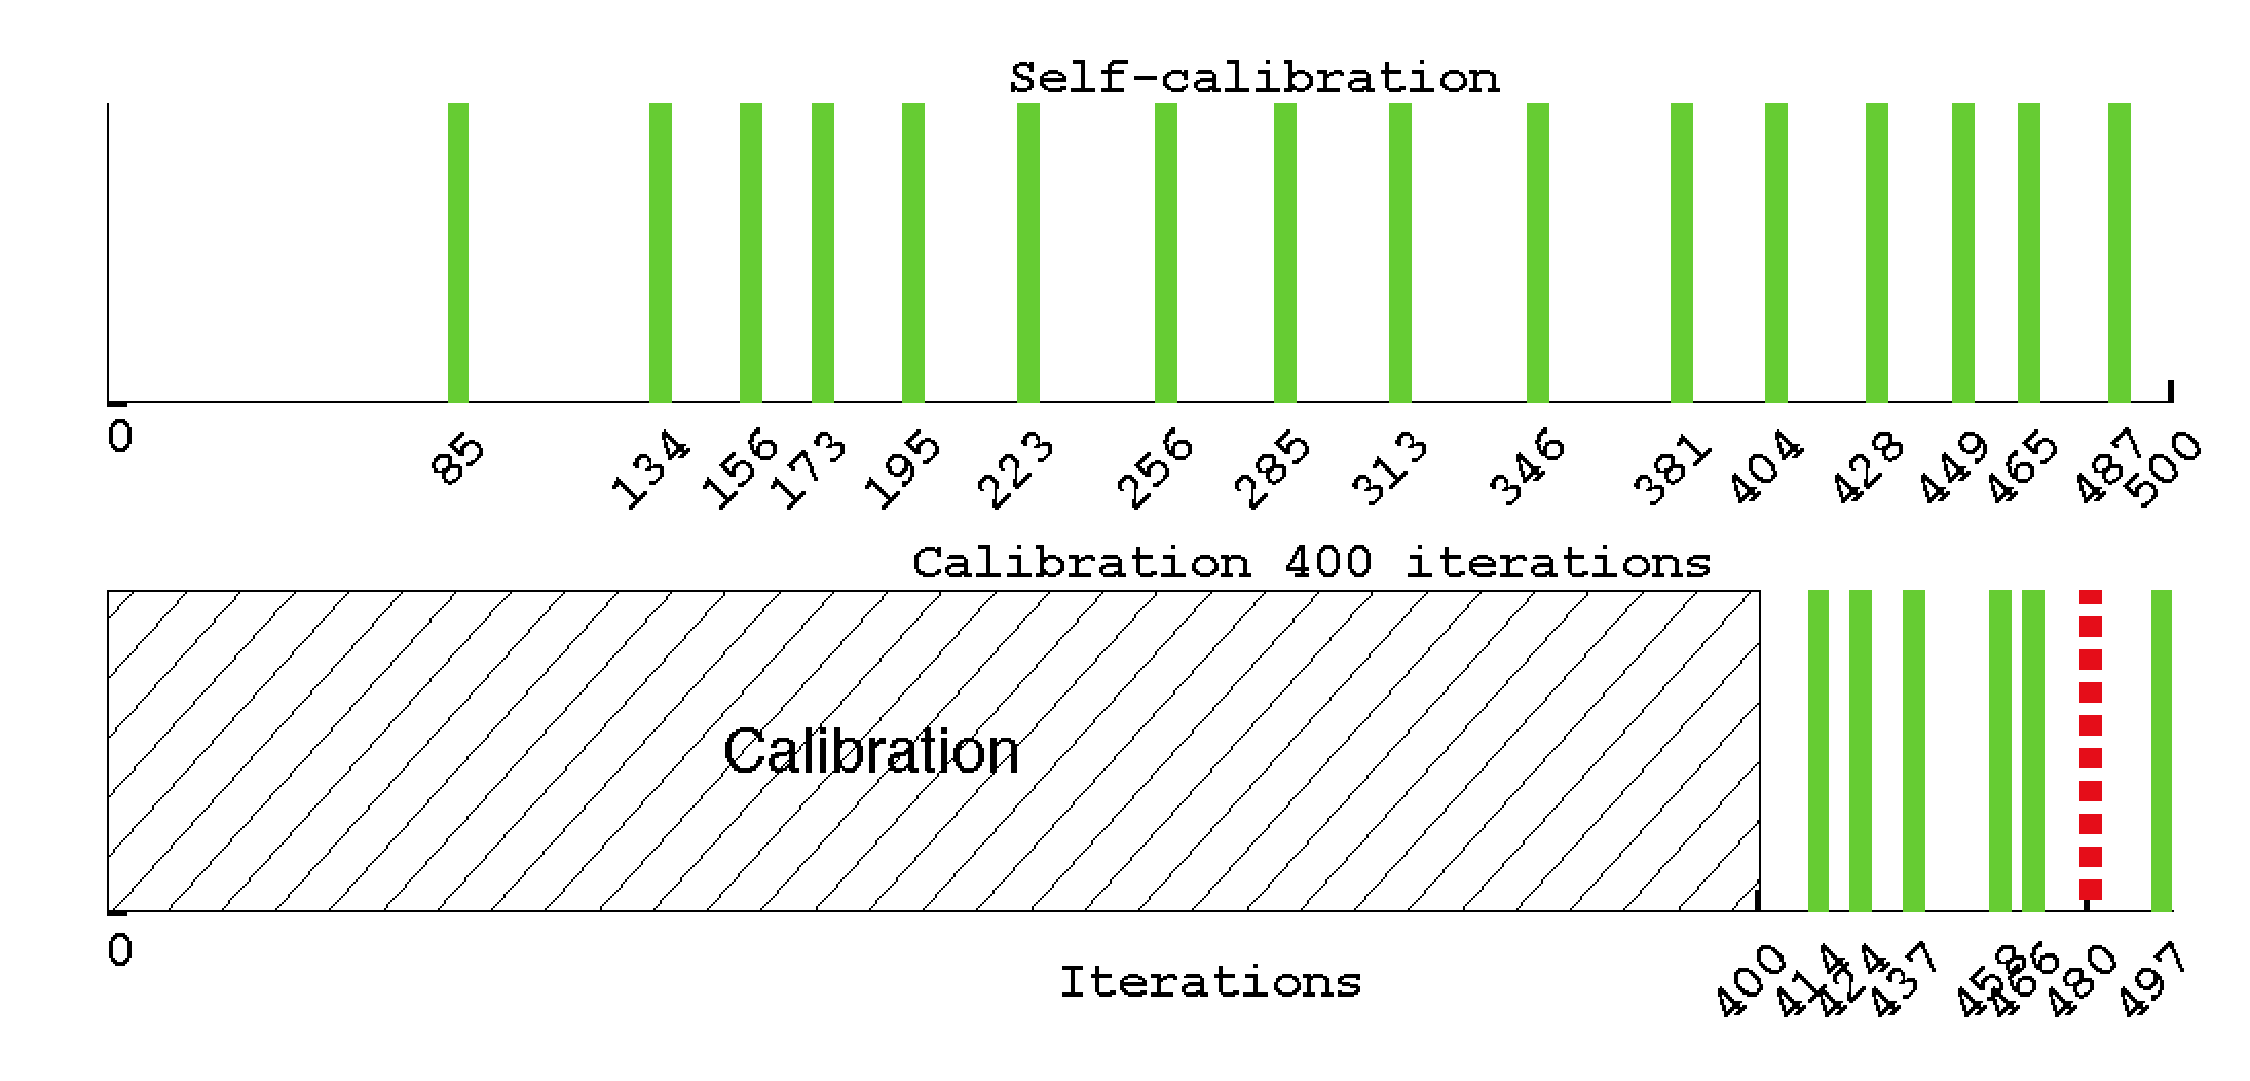
\includegraphics[width=\sequencesize\columnwidth]{\imgpath/plot_the_aaai_sequence.eps}
\caption{Nombre de tâche résolue dans le temps avec des données EEG. L'algorithme d'auto-calibration (haut) est comparé aux méthodes nécessitant une phase de calibration (bas, ici 400 itérations de calibration Le barres verte et rouge représente respectivement les bonnes et les mauvaise exécutions de la tâche par la machine. La méthode d’auto calibration proposée dans cette thèse permet de compléter une première tache plus rapidement, sans pour autant faire d'erreur.}
\label{fig:sequencefrench}
\end{figure}

Les même expériences on été testé avec des utilisateurs réel. Leur résultats confirme ceux de simulation et sont présenté au chapitre \ref{chapter:bci} ainsi qu'au chapitre \ref{chapter:limitations:overlap}. Nos résultats démontrent expérimentalement que notre approche est fonctionnelle et permet une utilisation pratique de l'interface plus rapidement. De plus notre système ne nécessite pas la présence d'une personne extérieure pour calibrer le système et est donc un candidat potentiel pour amener l'utilisation des interfaces cerveau machine dans les maisons.

\subsection*{Planification des actions}

Un autre résultat important de cette thèse est le planning est également différent des algorithmes précédemment développés. En effet une couche d'incertitude supplémentaire est présente, le sens des signaux est inconnu et nous disposons d'une multitude de candidat possible. Il faut donc inclure cette incertitude dans la mesure d'incertitude globale permettant de naviguer plus efficacement dans le monde. Afin de collecter des signaux varié. Les résultats présente au chapitre montre que notre méthode de planification des actions améliore significativement le temps nécessaire à l'identification de la tâche mais aussi à l'établissement du modèle de langage de l'utilisateur.
\ref{chapter:planning}

\subsubsection*{Extensions}

\ref{chapter:limitations:continousstate}
\ref{chapter:limitations:continuoushypothesis}
\ref{chapter:limitations:framehypothesis}
\ref{chapter:limitations:proof}


Au chapitre~\ref{chapter:limitations}, nous abordons et proposons des solutions à de multiples limitations de l'approche présentée dans cette thèse. Nous montrons d'abord qu'il est possible d'utiliser le système dans des espaces continue: premièrement pour un état continue du système mais sur un ensemble infini d'hypothèse sur la tâche. Par la suite, nous montrons que la connaissance a priori du protocole d'interaction n'est pas une limitation forte et que notre système peut détecter le protocole par l'interaction pratique avec l'utilisateur.

Etrangement, cette thèse ne traite pas directement du problème simple, symbolique, mais s'intéresse d'abord à une représentation non-symbolique des signaux de communications. Ceci dans un but applicatif à courts termes auquel de fastidieuses preuves mathématiques dans des domaines trop simplifiés n’auraient laissé guère de temps à l'expérimentation. Ainsi la formulation simple du labyrinthe présentée au début de ce résumé n'est adressé que dans la toute dernière section de cette thèse par une preuve de la validité de notre solution pour le cas de signaux de communication symbolique et sous de forte contrainte de l'environnement. Ce dernier développement montre que ce genre de problème peut-être modélisé mathématiquement et ouvre la voie de prochaine exploration plus théorique de ce problème. Permettant peut-être de trouver des  garantie plus grande sur la convergence et les performance de nos algorithmes. Bien que ce genre de preuve semble encore très limité pour l'interaction pratique de par la nature imprévisible du comportement humain.

% Finalement, nous démontrons mathématiquement sur un exemple simplifié et sous certaines conditions que notre méthode est garantie d'identifier la bonne hypothèse.

\subsection*{Expèrience humain-humain}

Une autre contribution de cette thèse et la mise en place d'un protocole expérimental pour analyser le comportement de deux humain mis dans la situation que doivent résoudre nos algorithmes (chapitre~\ref{chapter:humanexperiment}). Dans cette expérience deux humains doivent collaborer à l'exécution d'une tâche de construction. Ils ne peuvent interagir que par le biais d'une interface dont le sens des signaux transmis est inconnu et indéfini au départ pour les deux parties.

Il sera intéressant de voir la dynamique de construction d'un langage commun entre les deux participants. Langage qui n'était pas prévu au début de l'interaction s'établi de tel sorte qu'une personne extérieure à l'expérience ne pourra alors pas comprendre ce qui ce passe en observant le résultat final de l'interaction.

\subsection*{Conclusion}

La vision développée dans cette thèse est qu'il est possible pour une machine d'interagir avec un humain sans comprendre a priori la façon dont l'utilisateur communique l'information. Plus concrètement notre système n'a pas d'apriori sur le sens des signaux reçu et construit son modèle durant l'interaction pratique avec l'utilisateur sans jamais avoir accès a une source sûre d'information. Cela sera, nous l'espérons, le fruit de nombreux travaux futur.

Au delà du challenge technique de l'auto-calibration, des questions d'utilisation pratique et d'acceptabilité éclosent et sont présentées au chapitre~\ref{chapter:limitations:userstudies}. Parmi elles, la plus importante à tester en condition réelle est: Comment les utilisateurs vont réagir au fait que la machine, le robot, ne soit pas immédiatement réactif à ces ordres mais doivent apprendre le sens des signaux pendant l'interaction? En effet, même si nos algorithmes apportent une plus grande flexibilité d'interaction, ils ne permettent pas à l'utilisateur une fonctionnalité parfaite et immédiate du système qui doit en effet apprendre de l'interaction. Cette phase d'apprentissage pourrait être perçus comme une inopérabilité du système et par conséquent impacter l'intérêt et l'utilisabilité réelle de notre système.\\

\noindent {\large\textbf{Mots-clés:}} Auto-Calibration, Apprentissage par interaction, Interaction Humain-Robot, Interface Cerveau-Machine, Interaction Intuitive et Adaptative, Robotique, Acquisition de Symbole, Apprentissage Actif, Calibration.\\

Ce travail a été financé par INRIA, le Conseil Régional d'Aquitaine et la bourse ERC EXPLORERS 24007.
\NewPage

\cleardoublepage
%!TEX root = ../thesis.tex

\begin{titlepage}
\begin{center}
\noindent {\LARGE \textbf{INRIA BORDEAUX SUD-OUEST}} \\
\vspace*{0.3cm}
\noindent \textbf{\'ECOLE DOCTORALE MATH\'EMATIQUES ET INFORMATIQUE} \\
\noindent UNIVERSIT\'E DE BORDEAUX \\
\vspace*{0.5cm}
\noindent \Huge \textbf{P H D\ \ T H E S I S} \\
\vspace*{0.3cm}
\noindent \large {to obtain the title of} \\
\vspace*{0.3cm}
\noindent \LARGE \textbf{PhD of Science} \\
\vspace*{0.3cm}
\noindent \Large of the University of Bordeaux \\
\noindent \Large \textbf{Specialty : \textsc{Computer Science}}\\
\vspace*{0.4cm}
\noindent \large {Defended by\\}
\noindent \LARGE Jonathan \textsc{Grizou} \\
\vspace*{0.4cm}
\noindent\rule{10cm}{0.4pt}\\
\vspace*{0.4cm}
\noindent {\huge \textbf{\thesistitle}} \\
\vspace*{0.4cm}
\noindent\rule{10cm}{0.4pt}\\
\vspace*{0.4cm}
\noindent \Large Thesis Advisors: Manuel \textsc{Lopes} and Pierre-Yves \textsc{Oudeyer} \\
\vspace*{0.2cm}
\noindent \Large prepared at INRIA Bordeaux Sud-Ouest, \textsc{Flowers} Team\\
\vspace*{0.2cm}
\noindent \large defended on September 28, 2014 \\
\vspace*{0.5cm}
\end{center}
\noindent \large \textbf{Jury :} \\
\begin{center}
\noindent \large 
\begin{tabular}{llcclr}
      \textit{Reviewers :}	    & Mohamed \textsc{Chetouani}   & - & Prof.         & ISIR, UPMC          & HdR \\
				                & Mich\`ele \textsc{Sebag}     & - & DR            & CNRS                & HdR \\
      \textit{Examinators :}    & Fabien \textsc{Lotte}        & - & CR            & INRIA                     \\
      				            & Luis \textsc{Montesano}      & - & Assoc. Prof.  & Univ. of Zaragoza         \\
      \textit{Advisors :}       & Manuel \textsc{Lopes}        & - & CR            & INRIA-ENSTA               \\
                                & Pierre-Yves \textsc{Oudeyer} & - & DR            & INRIA-ENSTA         & HdR \\
      % \textit{President :}  & Nicholas \textsc{Ayache}      & - & INRIA (Asclepios)\\
      % \textit{Invited :}		& Hanna \textsc{Kafrouni}		& - & DOSISoft S.A.
\end{tabular}
\end{center}
\end{titlepage}
\sloppy

\titlepage

\NewPage

\cleardoublepage
%!TEX root = ../thesis.tex

\begin{vcenterpage}
% \noindent\rule[2pt]{\textwidth}{0.5pt}
\begin{center}
{\large\textbf{Acknowledgments\\}}
\end{center}


% It was all about people providing me with the opportunity to learn.

First of all, I would like to thank Pierre-Yves Oudeyer and Manuel Lopes for supervising me during this three years. 

And especially for giving me the opportunity to simply be in the lab, listening and taking part in various scientific and philosophical discussions.

I am grateful to Dr. Charles Capaday, Dr. Ram\'{o}n Huerta and Prof. Auke Jan Ijspeert for providing me with the early opportunity to discover research in their respective labs. Without them, I would never have pursued doctoral studies.

During these three years, I had the chance to engage in different collaborative works. I thank I{\~n}aki Iturrate and Luis Montesano for their numerous advises and their infinite patience. I thank Anna-Lisa Vollmer and Katharina J. Rohlfing for their invaluable insight on the implication of this work to human behavioral understanding. I thank Peter Stone and Samuel Barrett for their enthusiasm and for providing me the opportunity to visit the LARG lab.

I thanks the jury members 

Unlimited thanks to my family for the good start in life they gave me, my friends for they unique ability to make me laugh, and Sara Maubourguet for her support all along these three years.

Numerous thanks go to all the members of the \textsc{FLOWERS} team for contributing in making these three years a memorable experience. 

Didier Roy

Matthieu Lapeyre
Pierre Rouanet
Fabien Benureau
Olivier Mangin
Paul Fudal
Cl\'{e}ment Moulin-Frier
Steve Nguyen
Thomas Cederborg
Thomas Degris


Mai Nguyen
Adrien Barannes
Benjamin Cl\'{e}ment

Yoan Mollard
Thibault Munzer



As well as the numerous internship students whose sole evoquation of their names would fill this entire page.


This work has been supported by INRIA, Conseil R\'egional d'Aquitaine and the ERC grant EXPLORERS 24007.

 
% Without I{\~n}aki, running experiments involving brain signals would not have existed. He spent an uncountable amount of time sitting with the cup on and gel in the hair. Without Luis, my understanding of the problem would not . Him and Manuel were exceptionally patient when listening to my explanation. we would not have reached the same level of understanding of the problem.

% \noindent\rule[2pt]{\textwidth}{0.5pt}
\end{vcenterpage}
\cleardoublepage
%!TEX root = ../thesis.tex

\begin{vcenterpage}
% \noindent\rule[2pt]{\textwidth}{0.5pt}
% \begin{center}
% {\large\textbf{\thesistitle\\}}
% \end{center}
\begin{center}
{\LARGE\textbf{Abstract}} 
\end{center}

% \begin{center}
% \noindent\rule[2pt]{0.2\textwidth}{0.5pt}
% \end{center}
% \vspace{1cm}

This thesis investigates how a machine can be taught a new task from unlabeled human instructions, which is without knowing beforehand how to associate the human communicative signals with their meanings. The theoretical and empirical work presented in this thesis provide means to create calibration free interactive systems, which allow humans to interact with machines, from scratch, using their own preferred teaching signals. It therefore removes the need for an expert to tune the system for each specific user, which constitute an important step towards flexible personalized teaching interfaces, a key for the future of personal robotics.
% This thesis investigates how a robot can be taught what to do from instructions provided by a human without knowing beforehand how to associate the human communicative signals to their meanings.

Our approach assumes the robot has access to a limited set of task hypotheses, which include the task the user wants to solve. Our method consists of generating interpretation hypotheses of the teaching signals with respect to each hypothetic task. By building a set of hypothetic interpretation, i.e. a set of signal-label pairs for each task, the task the user wants to solve is the one that explains better the history of interaction.

% For this work, we consider different scenarios where a human teacher uses initially unclassified speech words, whose associated meaning can be a feedback (correct/incorrect) or a guidance (go left, right, up, \ldots). We consider different scenarios where a human teaches a robot to perform a new task using initially unclassified signals, whose associated meaning can be a feedback (correct/incorrect) or a guidance (go left, right, up, \ldots).

We consider different scenarios, including a pick and place robotics experiment with speech as the modality of interaction, and a navigation task in a brain computer interaction scenario. In these scenario, a teacher instructs a robot to perform a new task using initially unclassified signals, whose associated meaning can be a feedback (correct/incorrect) or a guidance (go left, right, up, \ldots). Our results show that a) it is possible to learn the meaning of unlabeled and noisy teaching signals, as well as a new task at the same time, and b) it is possible to reuse the acquired knowledge about the teaching signals for learning new tasks faster. We further introduce a planning strategy that exploits uncertainty from the task and the signals' meanings to allow more efficient learning sessions. We present a study where several real human subjects control successfully a virtual device using their brain and without relying on a calibration phase. Our system identifies, from scratch, the target intended by the user as well as the decoder of brain signals.



Based on this work, but from an other perspective, we introduce a new experimental setup to study how human behave in unconstrained asymmetric collaborative task. In this setup, two humans have to collaborate to solve a task but the channels of communication they can use are constrained and force them to invent and agree on a shared interaction protocol in order to solve the task. These constraints allow to analyze how a communication protocol is progressively established through the interplay and history of individual actions.

% Finally, we address a number of limitations and propose extensions to the problems of continuous state space, continuous task space, and unknown interaction protocols. 





% {\large\textbf{Keywords:}} Keyword 1, Keyword2.\\

% \noindent\rule[2pt]{\textwidth}{0.5pt}
\end{vcenterpage}
% \cleardoublepage
% %!TEX root = ../thesis.tex

\begin{vcenterpage}
\noindent\rule[2pt]{\textwidth}{0.5pt}
\begin{center}
{\large\textbf{Foreword\\}}
\end{center}

The purpose of this manuscript is to explain a problem and to provide an intuition on how to solve this problem. While reading, you will be introduced to the most important aspects of the work by simple, hopefully intuitive, visualization of the problem and of the specific properties we exploit. My aim is therefore to endow the interested readers to implement their own version of the algorithm with the tools they are more familiar with.

\noindent\rule[2pt]{\textwidth}{0.5pt}
\end{vcenterpage}

\tableofcontents
% \listoffigures
% \listoftables
\NewPage

\mainmatter

% %!TEX root = ../../thesis.tex
\define{\chapterpath}{\allchapterspath/introduction}
\define{\imgpath}{\chapterpath/img}

\chapter{Introduction}
\label{chapter:introduction}
\minitoc

This thesis investigates how a robot can be taught what to do from instructions provided by a human without knowing beforehand how to associate the human communicative signals to their meanings.

In the past decades, robotics and autonomous systems have seen tremendous improvement in their motor, perceptual, and computational capabilities. As a good example, we have been able to send and operate rovers for several years on the planet Mars (Spirit, Opportunity, Curiosity), which indicates the technologies are well mastered. However, getting such robots to do what we want them to do remains a skill of few, and bringing robotics system teachable by everyone and capable of social interaction in our daily life has been identified as the next milestone for the robotic community.

As for bringing computers in all our homes required easy and intuitive ways for people to make use of them, bringing robots in our daily life requires easy and intuitive ways for people to make robots do useful things for them. Currently, implementing advance behaviors in a robot, such as folding a shirt, requires similar skills than a computer scientist needed 50 years ago to build any application using punch cards, i.e. a lot of expertise, patience and trials and errors development. Due to the diversity of skills a robot should be able to execute in our daily environment, including interacting with humans and objects, traditional programming methods hinder the deployment of robotic system at homes and workspaces.

Instead, researchers are trying to endow robotic systems with the ability to learn from social interaction what tasks to execute and how they should be executed. Several methods have been considered to allow non-technical users to ``program'' robots, such as \emph{learning by demonstration} where the human demonstrate the skills to the robot, \emph{learning from reinforcement} where the human assesses the actions of the robot with respect to the aimed behavior, or \emph{learning from instructions} where the human explains the sequence of actions to performs in order to fulfill the task . Advances in these areas should allow the emergence of robot companions, living inside our homes providing assistance to the daily tasks, care, and entertainment. 

Endowing a robot with the ability to learn form interaction with a human partners requires to solve several challenges: the technical challenge of motor, perceptual and cognitive skills acquisition and generalization, the practical challenge of interacting in a social way with human being of different background. Especially, the robot must be able to understand the communicative signals from the human and communicate its own intention and ``state of mind'' back to the human. Additionally, as robots are embodied agent, the challenge of social acceptance of robot among people is an additional obstacle. A robot that is not accepted by people will not be used, and a robot that cannot be understood by people or a non-intuitive interface is likely to impact the performances of the learning systems developed.

Currently most of the challenges are considered in isolation. For example, when a robot learns a task from human instructions, it is assumed the robot receives instructions in a symbolic way, e.g. if the human uses speech to communicate his instructions the robot is assumed to be able convert raw speech into text. Similarly, when a robot learns how to recognize speech utterances, which is how to convert raw speech into a meaningful representation such as text, the robot is usually fed with many examples of speech utterances associated  with their symbolic representation.

In this thesis, we consider the two latter challenges simultaneously which is learning a new task from raw human instructions signals whose associated meanings are initially unknown. Solving this problem would allow the same robot to be taught by a variety of users using their preferred teaching signals and without the intervention of an expert to calibrate the system to the specific teaching signals used by each users. For example, a robot that accepts speech commands usually accept only one or a limited set of pre-specified speech utterances for each command, e.g. using the word ``forward'' to ask the robot to move forward. With the method described in this thesis, the user could use its preferred word to ask the robot to move forward, e.g. ``straight'' or ``up'', but also words whose usual meanings are non-related to the move forward action such as ``dog'', ``backwards'', or ``blue'', or interjection such as ``ah'', ``oh'', or even non speech utterance such as a hand clapping. The robot, after some practical interaction with the user, will find out which signal is associated to the action moving forward.

Our approach assumes the robot has access to a limited set of task hypothesis which include the task the user wants to solve. For example, if the user's goal is to guide the robot towards a specific room in a house, there is a limited number of possible tasks which are the number of rooms in the house. The idea behind our method consists of generating interpretation hypothesis of the teaching signals with respect to each hypothetic task. We will see that by building a set of hypothetic interpretation, i.e. a set of signal-label pairs for each task, the task the user wants to solve stands out by having the best coherence between the underlying spacial organization of the signals in their feature space and the labels associated to each signal. In others words, the correct task is the one that explains better the history of interaction.

In the following this introduction, we present in more details the challenges of learning from social interaction with humans and explicit the usual assumptions made when designing such systems. On this basis, we define the specific challenges addressed in this work and describe the contribution of the thesis.

%%%%%%%%%%%%%%%%%%%%%%%%%%%%%%%%%%%%%%%%%%%%%%
%%%%%%%%%%%%%%%%%%%%%%%%%%%%%%%%%%%%%%%%%%%%%%
%%%%%%%%%%%%%%%%%%%%%%%%%%%%%%%%%%%%%%%%%%%%%%
%%%%%%%%%%%%%%%%%%%%%%%%%%%%%%%%%%%%%%%%%%%%%%
%%%%%%%%%%%%%%%%%%%%%%%%%%%%%%%%%%%%%%%%%%%%%%
\section{Social Learning: Robot learning from interaction with humans}
\label{sec:intro:social}

It is often easier to acquire a new skill if someone that already acquired that skill teach us how to do it. The field of social learning in robotics investigates how knowledge can be transferred from humans to robots through social interaction. Social interaction implies the human interacts with the machine using similar modalities as when interacting with other human beings, for example using speech, gestures, or by demonstrating some behaviors. 

We can identify three main social learning paradigms used in robotics today: \begin{inparaenum}[(a)] \item learning from human demonstration, where the robot learns by imitating the human actions, \item learning from human reinforcement, where the robot learn from assessments on its own actions provided by the user, and \item learning from human instructions, where the robot learns from concrete instructions about what do to next provided by the user. \end{inparaenum}

Each of those paradigms requires to solve two main challenges: \begin{inparaenum}[(1)] \item the robot should be able to identify which parts of the interaction, and of the environment, are relevant to the acquisition of the new skill, and \item the robot should be able to infer, from the relevant informations extracted from the interaction, the new skill or task the human wants the robot to achieve. \end{inparaenum}

As we will see in the following subsections, most of the work in robot social learning considered those two latter challenges separately and most of the efforts focused on the second challenge of designing better learning algorithm.

% This approach contrast with the usual methods used to endow a robot with a new skill, such as directly programming the robot or defining a mathematical fitness function for that skill. 
% Social interaction, by being the most intuitive way for humans to communicate,   are the most intuitive way human communicative between each others and if robot are able
% By using speech, gestures, or by providing demonstration, human users can teach a robot a new skill without knowing how to program or how to define a fitness function this a particular skill. 
% This way human users can interact with machines without knowing how to program or how to define a fitness function for a particular task. People will be more familiar  of the desired skill, which correspond to more intuitive interaction for humans.

% In the following of this section we present three main social learning paradigms: \begin{inparaenum}[(a)] \item learning from human demonstration, where the robot learns by imitating the human actions, \item learning from human reinforcement, where the robot learn from assessments on its own actions provided by the user, and \item learning from human instructions, where the robot learns from concrete instructions about what do to next provided by the user. \end{inparaenum}

%%%%%%%%%%%%%%%%%%%%%%%%%%%%%%%%%%%%%%%%%%%%%%
%%%%%%%%%%%%%%%%%%%%%%%%%%%%%%%%%%%%%%%%%%%%%%
\subsection{Learning from human demonstrations}

Learning from human demonstrations, also called programming by demonstration or learning by imitation, is the process of learning a new skill from practical examples of how to perform a this skill \cite{schaal1999imitation,calinon2008robot,argall09survey,lopes10imitationchapter}. More formally, the robot should infer a policy which is a mapping between world states and actions by observing only a  some examples of state to action mapping, i.e. some demonstrations, which may be noisy and incomplete.

Following the survey of Brenna D. Argall \cite{argall09survey}, we will segment our presentation of learning from human demonstration in three parts, first we will present the different method used to collect training data, i..e to gather the demonstration, then we will present several methods allowing to derive a policy from demonstration, and finally we highlight some limitations of the method.

% Demonstrating a task to a robot is easier for the user than directly programming a behavior by writing lines of code. But creating a robot that learn from example requires to solves two main problems: \begin{inparaenum}[(1)] \item creating algorithm capable of inferring the user desired behavior from its demonstrations, but also \item allowing the robot to identify what part of the environment and of the human behavior are relevant to the task, i.e. to extract the information related to a demonstration from the interaction. \end{inparaenum}

\subsubsection*{Collecting demonstrations}

Collecting demonstration is probably the most important part in the learning process. Demonstration of good qualities will results in an easier learning while bad quality demonstrations are likely to impact the quality of the learned behavior.

We group the demonstration recording methods in two categories: \begin{inparaenum} \item teleoperation where the human demonstrate the skill by directly control the robot, and \item external observation where the robot is observing the human providing demonstration. \end{inparaenum} More formally, learning from data collected by a direct control of the robot by the human is called learning from demonstration, while learning from data collected by observing the human demonstrating the skill is called learning from imitation. We will see that this latter approach leverage some embodiment issues.

During teleoperation, the robot is directly operated by the teacher and therefore record the demonstration using it own sensors, i.e. the robot directly observe a sequence of state-action pairs in his own referential. It is the most direct and most efficient method to provide demonstration. However this method does not always apply well to all robots, for example, robot with many degrees of freedom can not be teleoperated efficiently by one person, but also robots that should maintain equilibrium are sometimes impossible to manipulate directly, such as demonstrating a walking behavior by teleoperating the legs of a humanoid robot.

Teleoperation has been used in a variety of robotic applications, including learning of aerobatic helicopter flight \cite{abbeel2007application}, object displacement with environmental constrained (e.g. obstacle avoidance) \cite{guenter2007reinforcement,calinon2007teacher}, object stacking \cite{calinon2007teacher}, or ball grasping on the Aibo robot \cite{grollman2007learning}.

When learning by imitation, the robot observe a human teacher demonstrating the skill. The fundamental difference with the teleoperation approach is the difference of embodiment between the human and the robot. This issue is referred as the correspondence problem \cite{nehaniv2002correspondence}, which the problem of mapping between the demonstrator actions (i.e. the human) and the imitator actions (i.e. the robot). For example, when demonstrating a gesture to a humanoid robot, the robot can not directly transpose the human movement to its own body as the human and the robot do not share the same body characteristic. If we consider a humanoid robot imitating the posture of a human demonstrator, the problem is better defined as reproducing the human posture as closely as possible while maintaining balance \cite{hyon2007full,yamane2009simultaneous}, where some additional constraint are provided to the robot by the system designer.

Recording the human demonstration can be done using a variety of sensors, either by adding sensors directly on the users (wearable sensors), either by using only the sensors non directly connected to the demonstrator body or relevant object. For example, using a motion capture device or using only a pair of video cameras situated in the robot's head.

Learning from imitation has been investigated in a variety of robotic application, including executing a tennis forehand swing \cite{ijspeert2002movement}, imitating arm movement \cite{billard2001learning} and hand posture \cite{chella2004posture}, object grasping \cite{lopes2005visual,tegin2009demonstration}, and also demonstration including a force component such as the fingertip force for grasping and manipulating objects \cite{lin2012learning}. Others works focused on learning by imitation a sequential task, which required to combine a sequence of multiple action to fulfill the task \cite{pardowitz2005learning,natarajan2011imitation}.

\subsubsection*{Inferring a policy}

Given a dataset of demonstration collected using one of the methods presented above, the robot should infer what action it should take in any given state to correctly fulfill the task demonstrated by the human. Learning can be as straightforward as reproducing the demonstrated behavior exactly, but most often, as the demonstration may be noisy or incomplete, the robot need to generalize from the example. We will differentiate between two approaches: \begin{inparaenum}[(a)] \item directly deriving a mapping between states and actions, i.e. a policy, from the observed data with the aim or reproducing the teacher policy, and \item the second one consist of inferring the human objective and, by using some planning method, reproducing the desired outcome without necessarily using the same actions as the demonstrator. \end{inparaenum} Roughly, the first approach is more suited for imitation while the second is more suited for emulation. 

The first approach resumes in approximating the policy function observed form the user behavior. Depending on the properties of the problem, the algorithms for learning the policy are either classification or regression techniques. 

\begin{itemize}

\item \textbf{Classification} methods are well suited for mapping discrete or continuous state to discrete actions. An example would be a robot learning to play a video game from demonstration, depending on the current state of the agent in the world, the robot should learn to press the appropriate buttons.

A large variety of classification algorithm has been used in learning form demonstration scenario. Among others, Support Vector Machines for a robot learning how to sort balls \cite{chernova2008teaching}, Hidden Markov Models have been used for an assembly task \cite{hovland1996skill}, Gaussian mixture models in a simulated driving domain \cite{chernova09jair}, but also neural networks \cite{mataric2000sensory}, beta regression \cite{montesano2009learning} or k-Nearest Neighbors \cite{saunders2006teaching}.

\item \textbf{Regression} method are well suited for for mapping discrete or continuous state to continuous actions. An example would be an autonomous car learning to steer the wheels from demonstration, given information about the surrounding environment the car should turn the driving wheel appropriately.

A large variety of classification algorithm has been used in learning form demonstration scenario, they mainly applied for learning trajectories from noisy demonstrations. Among others, Gaussian Mixture Regression for generalizing trajectories from examples in different applications \cite{calinon07}, Locally Weighted Regression for learning to produce rhythmic movement using central pattern generators \cite{schaal1998programmable,ijspeert2002learning}, Neural Networks for learning autonomous driving \cite{pomerleau1991efficient}, or Incremental Local Online Gaussian Mixture Regression for imitation learning for learning incrementally
and online new motor tasks from demonstration \cite{cederborg2010incremental}.

\end{itemize}

The second approach consists of inferring the goal of the human from demonstration. By expressing this goal as an optimization problem or as a reward function, the robot can learn to reproduce the human goal by its own means.

\textbf{Inverse reinforcement learning} \cite{ng2000algorithms,Abbeel04icml} is a popular method that is inferring the hidden reward function the demonstrator is trying to optimize based on its demonstrations. In addition, the demonstrations can be used to learn a model of the environment in state unreachable to robot by mere self-exploration. Once the reward function has been evaluated form the demonstration, and given the dynamic of the environment, the robot can generate a plan to fulfill the task using his own ability. This method is especially interesting when the human and the robot do not have the same abilities. As an example, a robot may be able to execute a skill faster that a human, be mere reproduce of the human gesture the robot would not reach the same level of performance than by inferring the underlying goal of the human.

One of the most impressive achievement of the past decade used inverse reinforcement learning methods for the learning of aerobatic helicopter flight \cite{abbeel2007application}. Demonstration were provided by an expert pilot teleoperating, i.e. flying, the helicopter to help finding its dynamics and the fitness function corresponding to different maneuvers such as flip, roll, tail-in and nose-in funnel.

\subsubsection*{Limitations and assumptions}

The performance of the learning system is obviously linked with the quality of the information provided by the demonstration. Among others aspect, if some important state-action pairs have not been demonstrated or if the demonstration were of poor quality, i.e. including a lot of noise or being suboptimal or ambiguous in certain areas, the learner will be unable to generalize properly from the data. 

Unfortunately, in many cases, the demonstration are collected beforehand and sent to the learning algorithm in a batch way which do not allow the robot to have access to better demonstration. A potential solution is to ask the teacher for new demonstrations in those state where demonstration are missing or uncertain \cite{chernova2008multi,chernova09jair}, we will details more this approaches in the next chapter.

An other problem that of identifying what the human is really demonstrating. For example, if a human is demonstrating how to fish to a robot, is the human demonstrating the precise movement of the fishing rod or demonstrating where to place the float stopper in order to catch more fish. In other words, should the robot imitates the movement of the rod fishing movement or should it emulates the position float stopper. Where imitation is the act of reproduce the human demonstration in all details, and emulation is the act of fulfill the same goal than the human demonstrated. 

This problem is currently unsolved in the robot social learning literature and in practice the robot is explicitly told whether to imitate or emulate the demonstration. The problem of understanding what to do from the interaction with human is usually solved at design time, where the system design apply a multitude of constrain the the interaction with the robot such that no uncertainty or ambiguity remains on the demonstration. For example, the demonstrated movement and provided in isolation and contains only information about the task to be learned, similarly, the robot is explicitly ``told'' that the demonstration refer to such and such object and that it is for example a grasping task. Of course saying that the robot is ``told'' about the interaction is misleading, it is rather the all system that is constrained to optimize only a specific objective.

In the context of learning from human demonstration, four central questions are often predefined at design time: who, when, what, and how to imitate \cite{nehaniv2000hummingbirds}:

The \textbf{who} question refers to the problem of identifying who to imitate, It may refer to finding which person is currently providing demonstration, but also which person is better at providing accurate demonstrations of the task. This question has not been throughly investigated in the literature so far. One of the few work tackling this problem consider a finite set of teacher and select the most appropriate one based on the robot current learning rate \cite{Nguyen2012PJBR}. This method allows the robot learner to take advantage of the different levels of skills each teacher provide.

The \textbf{when} question refers to the problems of social coordination between the two partners, such as the turn-taking ability. For example, this aspect has been investigated in human-robot drumming activities where turn-taking and role switching are important component of a successful interaction \cite{weinberg2006robot,kose2008emergent}. The when question also applies for cases where the robot should decide whether to try to imitate its human partner or to explore the environment by itself \cite{chernova09jair,Nguyen2012PJBR}. 

The \textbf{what} question refers to the problem of identifying the important aspect of the demonstrations. It refers for example to the dilemma between imitation at the action level or emulation at the effect level. At the action level, the aim of the robot would be to reproduce the demonstrator action in the same way and in the same order. At the effect level, the robot should understand the underlying purpose associated to the action of the human. 

The latter problem of identifying the effect level of imitation depends on the context in which the interaction takes place. In particular the concept of affordances \cite{gibson1986ecological} --- which encode the relation between actions, objects and, effects --- is of primordial importance for the robot to be able to reproduce demonstration at the effect level. Several works have consider affordances for human-robot learning, among others they have been used to recognize demonstrations, decompose them in a sequence of subgoals and finally reproduce them \cite{macl07affimit}. Montesano et al. presented a method to learn affordances by interacting with several objects \cite{montesano2008learning}. The robot was able to extract relation betweens its actions, the objects, and the effects it produces using Bayesian inference methods.

While most of the time the interaction protocol is well constrained such that there is no ambiguity about which aspect of the demonstration should be imitated, some social cues can be used to infer which parts of a demonstration are relevant, such as the temporal differences of demonstration parts. Pauses during interaction have been shown to be linked to important key points in a task demonstration, and allow to extract subgoals or determine when a demonstration is completed \cite{theofilis2013temporal}.

The \textbf{how} question refers to the problem of determining how the robot will actually perform the behavior so as to conform with the metric identified when answering the what question. When the demonstration is only relevant at the effect level (emulation) the robot can solve the task by its own mean as soon as the objective is identified. However when the imitation is important at the action level (imitation), differences between robot and human morphology and capabilities makes solving the how question not straightforward. This latter issue has been discussed previously and is referred to as the correspondence problem \cite{nehaniv2002correspondence}, which the problem of mapping between the demonstrator and the imitator.

\transition

As stated before, the who, when, what, and how questions are usually skipped over in practical application and the data are provided already pre-formatted for the robot.

In the next subsection we present an other paradigm for social learning in robotics, the \emph{learning from human reinforcement} approach. In this paradigm, the human never demonstrates the task to the robot but rather observe the behavior of the robot and reinforce or punish some of its actions in order to shape its final behavior. We also call this approach learning from human feedback, where feedback implies a positive or a negative assessment of the robot's actions.

%%%%%%%%%%%%%%%%%%%%%%%%%%%%%%%%%%%%%%%%%%%%%%
%%%%%%%%%%%%%%%%%%%%%%%%%%%%%%%%%%%%%%%%%%%%%%
\subsection{Learning from human reinforcement}

Learning from human reinforcement, also called shaping, is the process of learning a new skill by receiving assessment over our actions In this paradigm, the human never demonstrates the task to the robot but rather observe the behavior of the robot and reinforce or punish some of its actions in order to shape its final behavior. We also call this approach learning from human feedback, where feedback implies a positive or a negative assessment of the robot's actions. Clicker training is a subclass of this problem that consider the human can only send positive reinforcement.

Pioneers works in this domain include the work of Blumberg et al. \cite{blumberg2002integrated} which trained a virtual dog to learn several sequential tasks and associate them with
verbal cues using clicker training method. Kaplan et al. \cite{kaplan2002robotic} applied similar method to teach an AIBO robot dog. An other pionners work considered a software agent, named Cobot, that resides interact with human agents in an online chat community called LambdaMOO. Cobot adapts its behavior from various source of feedback (reward or punishment) provided by human engaged in the chat community \cite{isbell2001social}.

This social learning paradigm has share many aspects with reinforcement learning \cite{sutton1998reinforcement}. In reinforcement the agent goal is take actions so as to maximize the cumulative reward. We make a difference between reinforcement learning algorithm and learning from human reinforcement in the sense that the nature of the reward information can not be treated the same way when it is provided by a human. For example, reward signals from human are frequently ambiguous and deviates from the strict mathematical interpretation of a reward used in reinforcement learning \cite{thomaz2008teachable,Cakmak2010optimality}. We will provide more details about human teaching behaviors in the next chapter but we note that this problem requires to develop new algorithms to monitor and handle the teaching style of each user.

Therefore recent works started to investigate how to additionally learn the way the human are providing feedback at the same time as the robot learn the skill \cite{knox2009interactively}. 

However, as for learning from human demonstration, the robot should be able to infer to which actions the human feedback relates to. It may also need to differentiate between different levels of feedback as some actions may be mandatory to complete the task while others may just be preferences from the users. In addition the user could make mistakes in its assessment or may not perceive the problem as it is modeled by the robot, therefore making inconsistent feedback. And as for most learning from demonstration, most of the works presented above consider predefined and restricted interaction so as to be able to map easily the human reinforcement with the robot's actions. Similarly, if the human is providing feedback using speech commands, there exist a system that translate speech utterances into a meaningful feedback information, e.g. mapping the word ``good'' to a positive reward.

\transition

As stated above, the who, when, what, and how questions are also applicable to learning from human reinforcement problem. This question are usually skipped over in practical application and the data are provided already pre-formatted for the robot.

Providing only reinforcement signals to a robot can be limiting, especially when the state space is large which increase the learning time and results in a laboring interaction between the human and the robot. In the next subsection we present an other paradigm for social learning in robotics, the \emph{learning from human instructions} approach. In this paradigm, the human never demonstrates the task to the robot but rather observe the the behavior of the robot and provide clues, which we will call guidance, about what action to perform next.

%%%%%%%%%%%%%%%%%%%%%%%%%%%%%%%%%%%%%%%%%%%%%%
%%%%%%%%%%%%%%%%%%%%%%%%%%%%%%%%%%%%%%%%%%%%%%
\subsection{Learning from human instructions}

Learning from human instructions, also called learning from advice, is the process of learning a new skill by receiving explicit instructions about what to do next. In this paradigm, the human never demonstrates the task to the robot but rather observes the behavior of the robot and provide clues accordingly in order to shape the robot final behavior. We also call this approach learning from human guidance, where guidance implies the user explicitly indicates to the robot what action to perform next.

In most scenario, advises are additional pieces of information allowing to improve the learning time and efficiency of an agent. It is therefore often combined with reinforcement learning algorithms where the advises influence the exploration behavior of the agent or influence directly the value of particular actions. 

In \cite{clouse1992teaching} and \cite{maclin2005giving} the teacher can influence the action selection of the agent by providing advice about preferred actions. In  \cite{smart2002effective} the trainer directly controls the agent action at important key states and let the agent learn the fine details. In \cite{kolter2007hierarchical}, the authors introduce a hierarchical apprenticeship learning method for teaching a quadruped LittleDog robot to walk on rough terrains. Their method differs from standard inverse reinforcement learning methods; rather than providing full demonstrations of the skill they consider human advices about single low level actions of the problem. More precisely, the expert indicates foot placement in situation where the robot made suboptimal foot step.

It is important for the robot to be able to generalize to previously unseen situation. In \cite{lockerd2004tutelage}, the robot Leo learns to switch all buttons on or off from human vocal instructions. When a new button is introduced in the environment the robot autonomously generalizes from the instructions and presses all buttons, instead of pressing only the one it was instructed to in the first place.

As for other learning paradigms, the robot should be able to infer to which part of the environment matters for the instructions, if the instructions can be generalized or not to other objects in the environment, if the instructions are related to what the robot should do next or what it should have done before, or in which referential are  instructions given. Ideally the robot should also keep track of other social signal received from the human, such as whether the user is really paying attention to the scene or whether the user can see the part of the space the robot is in. And as for other methods, most of the current works consider predefined and restricted interaction so as to be able to map easily the human instructions with the current important aspects of the environment and of the interaction.

\subsection{Discussion}

Our categorization of social learning paradigms  in three categories does not reflect the many subfamilies that exist between these categories, including those that are shared among categories. It is meant to situate the social learning problem in a more global picture, providing some interesting pointers for the interested readers. 

As we noticed, in most of the above presented work, the human and the robot had either no direct interaction with the robot, either few  highly constrained interactions. For example, the human demonstrations are provided in a batch perspective where data acquisition is done
before the learning phase. In the following section, we detail the usual assumptions made in most human robot interaction scenarios, and based on our observation we define the global challenge addressed in this thesis.

%%%%%%%%%%%%%%%%%%%%%%%%%%%%%%%%%%%%%%%%%%%%%%
%%%%%%%%%%%%%%%%%%%%%%%%%%%%%%%%%%%%%%%%%%%%%%
%%%%%%%%%%%%%%%%%%%%%%%%%%%%%%%%%%%%%%%%%%%%%%
%%%%%%%%%%%%%%%%%%%%%%%%%%%%%%%%%%%%%%%%%%%%%%
%%%%%%%%%%%%%%%%%%%%%%%%%%%%%%%%%%%%%%%%%%%%%%
\section{Usual Assumptions}

As we have seen, in most of the work in social learning there is a strong decoupling between the process of extracting useful information from the interaction and the process of learning and generalizing a new skill or task from those useful information.

On the one hand, if the goal of the robot is to learn a new task, the robot will be fed with the relevant interaction data formatted exactly in the format needed by the learning algorithm. For example, if a user should teach a robot to navigate in a maze, the protocol of interaction between the human and the robot will be ticked to match the need of the algorithm. The interaction will be turn by turn such as it is easy to associate user's instructions to robot's states. But the user will also be asked to comply to the specific signals the robot understand, such as using the word ``right'' and ``left'' to mean respectively ``right'' and ``left''.

On the other hand, when we want to learn some part of the user behavior, the task the users wants to achieved is assumed to be known. This allows to interpret the behavior of the user in the light of the known objective he is pursuing. This process is usually called a calibration phase and it is necessary to provide the robot with the ability to translate human communicative signals, such as speech or gestures, in a symbolic meaningful representation. For example, if we want our robot to learn which word the user uses to mean ``right'' and ``left'', we will ask the user to guide the robot in a maze following a specific path. The robot, knowing the path intended by the human, could identify that the human uses the word ``right'' and ``left'' or ``droite'' and ``gauche'' to mean respectively ``right'' and ``left''.

Therefore interacting with a robot present a chicken an egg problem. To teach a robot a new task, the robot must be able to understand the behavior of the human. But to come up with an understanding of the behavior of the human the robot must known what is the user overall objective. In this thesis, we present methods to overcome this chicken and egg problem in some specific cases. Before entering into more details, we should introduce a number of concepts that we will use in the following of this thesis.

\subsection{Interaction frames}

We start be defining the concept of interaction frame. An interaction frame is a structure that define all the aspects of the interaction that are pre-defined by the system designer and assumed to be followed by the human and the robot during the interaction.

The concept of interaction frame is a subclass of the more general concept of frame applied to the specific case of interaction scenarios. Frames are a concept that emerges simultaneously in social theory \cite{goffman1974frame} and artificial intelligence \cite{minsky1974framework}. They represents a stereotyped situations, a schema of interpretation given a particular situation or event. It is answering the question: \emph{what is going on here ?}, in order to reduce ambiguity of intangible topics by contextualizing the information. It creates a common ground about the purpose of the interaction \cite{tomasello2009cultural,rohlfing2013learning} and include ``predictable, recurrent interactive structures'' (\cite{ninio1996pragmatic}, p. 171). Frames thus provide interactants with guidelines about how to behave (a protocol for interaction) and also help interactants to understand the communicative intentions of their interaction partner.

The interaction frame is often implicitly assumed in robot learning experiments. We start by examplifying a few number of interaction frames and then provide a more formal description of an interaction frame.


One example of an interaction frame would be a human presenting an object to a robot at the same time as saying the name of the object. Being aware of this frame, the robot knows the utterance corresponds to the name of the object (and not its shape or its color). In this case, the label corresponding to the speech signal is given.

\paragraph{Feedback frame}
An other scenario is that of a human supervising the work of a builder robot. This builder robot is able to stack several blocks in order to form complex structures. The human wants the robot to build a specific construction but can not directly communicate the high level description of the structure to the robot. The robot only accept information about the quality of its last action. For example, if the robot took a blue cube and put it on top of a green cube, the human can assess this action and inform the robot that this particular stacking action was ``correct'' or ``incorrect'' according the human final structure wishes. After many interactions the robot is able to build the correct structure. We call this specific interaction scenario a feedback frame, where a feedback signals is defined as providing an information about the optimality of the action the robot just performed. A feedback signal can only take two values either ``correct'' or ``incorrect''.

\paragraph{Guidance frame} An other example is that of a human providing discrete action advice to a robot in the context of a reaching task. Concretely, if the human wants its robot to reach a specific room in the house, he will explicit tell the robot which direction to go in order to reach that room. For example asking the robot to go ``right'', ``left'', ``forward'', or ``backward''. The robot knows the signals of the user correspond to action it should perform to achieve the user intended goal. However the robot is not teleoperate and remains the one that select which action to perform given the advice of the teacher. For example, once the robot understood which room the user has in mind, it can go there directly without waiting for further guidance signals. We call this specific interaction scenario a guidance frame, where a guidance signals is defined as giving an information about what action to perform next.

The two latter feedback and guidance frame will be central to the future development of our work. For convenience we will refer to both feedback and guidance signals as instructions signals, in the sense that a teacher is instructing the robot using signals that may includes both feedback or a guidance instructions towards a final goal.

In our above examples, we have seen that an interaction frame regulates the interaction between the human and the robot. It includes both the constraints related to the task, e.g. teaching a robot which state to reach among a finite set of states, and the protocol used by the teacher to communicate to the robot, e.g. the teacher is assessing the robot's actions. In the context of this work, we separate the interaction frame definition in three categories:

\begin{itemize}

\item \textbf{The set of possible meanings the human can refer to.} As depicted before, a set of meaning may include ``correct'' and ``incorrect'' for those cases where the user is assessing the robot's actions. It could also be the set of action names for those case where the user provides guidances on what to do next.

\item \textbf{Details and timing of the interaction:} it corresponds to when and how the user will provide instruction signals. For example, the human sends a signal to the robot after every robot's actions. An other example is a human providing a feedback signal between 0.2 and 2 seconds after the robot's action he is referring to, like in \cite{knox2009interactively}.

\item \textbf{Constraints on the possible tasks:} The general context of the teaching process is known by the both the human and the robot. For example the robot is aware that the human wants it to reach a specific room in the house. And not to take an object in the fridge for example. This limits the number of hypothesis the robot can create about what the user has in mind.

\end{itemize}

In addition, the robot is assumed to be able to translate the communicative signals from the human into their respective meanings. For example if the human communicates to the robot using speech, then it is assumed a speech to text system is implemented and allow to convert the raw speech data into a symbolic representation.

\todo{too early}

In light of our observations, we define a generic frame function that, given a context of interaction and a task, returns the meaning intended by the teacher:
%
\begin{eqnarray}
Meaning = Frame(Context, Task)
\end{eqnarray}
%
Following our previous example, stating that if the robot moves from state 3 to state 4 (context), and that the human wants it to go in G1 (task), then the signals received from the human means ``incorrect'' (meaning), we can exemplify the use of the frame:
%
\begin{eqnarray}
``incorrect" = Frame((s3 \rightarrow s4), G1)
\end{eqnarray}





By making the interaction frames explicit, we can revise our understanding of the challenges associated to social learning. This might help us design machines more flexible to loosely defined interaction frames, or even machine that can learn the frames themselves.

A more formal description of a frame and a extended reflexion on how to leverage from more aspect of an interaction frame is presented in the thesis work of Thomas Cederborg. \todo{cite Thomas C.}


find some framework and cite thomas \cite{cederborg2013language}

\todo{make a list of many qestion that can be asked in that scope and refer to the question asked and studied in the thesis pf thomas C.}


In this work, we remove only one specific information from the frame, the ability to translate raw signals form the users to a meaningful representation for the robot. We call this kind of frame \emph{Unlabelled interaction frames} and we study how a robot can learn to cope with this lack of information. 

\subsection{Unlabelled interaction frames}

In previous section~\ref{chapter:humanexperiment:frames}, we defined the terms of interaction frames which represents a stereotyped situations, a schema of interpretation given a particular situation or event. Such frame is often assumed to be known by both the human and the robot.  which includes the signal-to-meaning classifier that translate the actual human signals into meaningful symbols for the robot. By comparing what the frame predicts and what the human actually said the robot can change its understanding of the situation.

Learning from unlabeled interaction frames correspond to the problem where the signal-to-meaning classifier is not given, and therefore the robot can not rely on a direct comparison between the prediction from the interaction frame and the observation from the human teacher.

What remains is the frame. It is at the core of our approach, it is assumed to be known by both the human and the robot. It includes both the constraints related to the task, e.g. teaching a robot which state to reach among a finite set of states, and the protocol used by the teacher to communicate to the robot, e.g. the teacher is assessing the robot's actions. Therefore, the meanings of the unlabeled signals is not explicitly given but is known to belong to a finite set of possible meanings.

We define a generic frame function that, given a context of interaction and a task, returns the meaning intended by the teacher:
%
\begin{eqnarray}
Meaning = Frame(Context, Task)
\end{eqnarray}
%
Following our previous example, stating that if the robot moves from state 3 to state 4 (context), and that the human wants it to go in G1 (task), then the signals received from the human means ``incorrect'' (meaning), we can exemplify the use of the frame:
%
\begin{eqnarray}
``incorrect" = Frame((s3 \rightarrow s4), G1)
\end{eqnarray}

\transition

The idea of unlabeled interaction frame summarizes the problem of interaction we tackle in this work. However it is a quite general concept, and in order to understand the underlying principles of our algorithm, in the following sections we will restrict our analysis to simple frames and simple worlds. We will also explicit a number of assumptions related to this work.

The first assumption is that the robot and the human are aware of the frame in which the interaction take place. This frame regulates the interaction between the two partners, it includes:

\begin{itemize}

\item \textbf{The set of possible meanings the human can refer to.} As depicted before, the set of meaning includes ``correct'' and ``incorrect'' for thoses cases where the user is assessong te robot's actions. It could also be the set of action names for those case where the user provides guidance on what to do next.

\item \textbf{Details and timing of the interaction:} it corresponds to when and how the user will provide instruction signals. For example, the human sends a signal to the robot after each action the robot performs. An other example may be the human providing a feedback signal between 0.2 and 2 seconds after the robot's action he is referring to, like in \cite{knox2009interactively}.

\item \textbf{Constraints on the possible tasks:} For example the robot is aware that the human wants to have it grasp one object on the table. And not reach for an object in a different room. This limits the number of hypothesis the robot can create.

\end{itemize}

By combining those three aspects of an interaction frame, the robot can create a set of interpretation hypothesis for the received teaching signals. For one possible task, and given a specific context (e.g. state and action performed in the environment), the robot can infer the meaning intended by the human user. By doing so for each possible task, it creates a set of interpretation hypothesis, which we rely on to fond the task taught by the user, as well as the signal to meaning mapping.


\section{Thesis Contributions}

The main contribution of the thesis is a method allowing a robot to learn from unlabelled interaction frame. In practice, it allow a user to start teaching a robot a new task using its own preferred teaching signals. For example, a user provides, using for example speech commands, instructions to a robot about what action to perform next, with our method, the user is not restricted to a pre-defined set of words and can rather use its preferred words. The system will learn which words are associated to which meaning as well as identifying the task the user wants to solve. The user could therefore use words in english, french or spanish, but also interjections or even hand clapping.

In more details, we can highlight four important contributions of this thesis:

\begin{itemize}

\item We propose a new experimental setup to study the co-construction of interaction protocols in collaborative tasks with humans \cite{vollmer2014studying} (chapter~\ref{chapter:humanexperiment}). In this setup, an architect and a builder must communicate using a restricted 10-bit channel in order to achieve the joint activity of constructing a structure using simple building blocks. We report experiments with human subjects which indicates that the kinds of meanings the participants coordinate on is limited some specific subsets such as feedback (``yes'', ``no''), guidance (``left'', ``right'', ``assemble''), feature based (``red'', ``small''), or global (``end'', ``reset'') instructions. Especially most of the user seems to concentrate on the ``yes'' and ``no'' kind of instruction. Finally we report that humans solve the problem by projecting the interaction into different common frames of
interaction, which is the basic principle used in the algorithms presented in this thesis.

\item  We present an algorithm that allow to simultaneously learn a new task from human instructions as well as the mapping between human instruction signals and their meanings \cite{grizou2013interactive,grizou2013robot,grizou2014robot,grizou2014calibration,grizou2014interactive} (chapter~\ref{chapter:lfui}). In practice, it allows a user to start teaching a new task to a robot using his preferred teaching signals and without going through the usual calibration phase.  

Our method consists of generating interpretation hypothesis of the teaching signals with respect to a set of possible task. We will see that the correct task is the one that explains better the history of interaction. We demonstrate the efficiency of our method in a pick and place scenario where a user use spoken words to instruct the robot to build a specific construction. We show that our method works if the teacher provide feedback (``correct'' or ``incorrect''), or guidance (``left'', ``right'', \ldots) instructions to our robot. Finally we show that our system can reuse the knowledge acquired about the signals of the users during the learning of a first to learn a second task faster.

\item We propose a measure of uncertainty on the joint task-signal space that takes into account both the uncertainty inherent to the task, which is unknown and remains to be estimated, as well as the uncertainty about the signal to meaning mapping, which is also unknown and remains to be estimated \cite{grizou2014calibration,grizou2014interactive} (chapter~\ref{chapter:planning}). Measuring uncertainty allows to optimize the action selection of our agent which improves significantly the learning time.

\item We apply our algorithm to brain computer interfaces (BCI) \cite{grizou2013zero,grizou2014calibration} (chapter~\ref{chapter:bci}). We present experiments where several subjects control an agent from scratch by mentally assessing the agent's actions and without requiring a calibration phase to train a decoder of the user's brain signals. In all experiments, our algorithm was able to identify a first task in less iterations that a usual calibration procedure requires.

\end{itemize}

\section{Thesis Outline}

The first aim of this manuscript is to explain the problem of learning from unlabeled interaction frames and to provide an intuition on what properties can be exploited to solve this problem. We will introduce the most important aspects of the work by simple visualization of the problem and of the specific properties we exploit. Our objective is therefore to endow the interested readers with sufficient understanding of the problem to implement their own version of the algorithm with the tools they are more familiar with.

In chapter~\ref{chapter:relatedwork}, we present an overview of the related work which span from language acquisition to brain computer interfaces.

In chapter~\ref{chapter:humanexperiment}, we introduce a new experimental setup to study the co-construction of interaction protocols in asymmetric collaborative tasks with humans. By presenting preliminary results based on this setup, we derive interesting lessons for our problem. This work on human experiment is a joint collaboration with Anna-Lisa Vollmer and Katharina J. Rohlfing.

In chapter~\ref{chapter:lfui}, we introduce in more specific terms the problem and provide a visual intuition on what properties we will exploit. We continue by formalizing the problem in a probabilistic framework, describe how each subcomponent of our algorithm are implemented and present results from a robotic pick and place scenario.

In chapter~\ref{chapter:planning}, we introduce the planning specificities related to our problem and provide a visual intuition on what properties we should track. We continue by defining the uncertainty measure used in the planning process and demonstrate on a 2D grid world problem the efficiency of the method with respect to other planning strategies.

In chapter~\ref{chapter:bci}, we present an application of the algorithm to a BCI scenario where a subject control an agent on a grid. We report online experiment showing that our algorithm allows untrained subjects to start controlling a device without any calibration procedure and by mentally assessing the device's actions. This work on BCI is a joint collaboration with I{\~n}aki Iturrate and Luis Montesano.

In chapter~\ref{chapter:limitations}, we discuss a number of limitations and propose several methods to overcome them. The limitations include the use of a discrete state space, the need for a finite set of task hypothesis and the fact that the interaction frame is uniquely defined in advance. We further propose a proof for our algorithm in restricted conditions.
% %!TEX root = ../../thesis.tex
\renewcommand{\chapterpath}{relatedwork}
\renewcommand{\imgpath}{\chapterpath/img}

\chapter{Related Work}
\label{chapter:relatedwork}
\minitoc


Why: So that audience can implement their own version of the algorithm. It means they should be convince it is a useful algorithm, known when to use it, be aware of the many assumptions and understand the underlying principle. 

There is only one simple idea to understand for the algorithm and one for the planning. I want to illustrate them using visual example. It should be the same all along the thesis. The T world seem the simplest one that shows the main element for feedback instructions. for the guidance it may be a bit more difficult.

Who: Specialist, the two reviewers that will read the thesis and PY and Manuel so they let it go. No self-estime here. I will use the term we in most of the thesis cause the work is a common reflexion from people in and around the lab.

What: intro and related work cause it is necessary for the "who" guys. Brief motivation from the human experiment, then visual explanation of the problem, first a dummy symbolic one with maybe a proof followed by a 2D signal feedback one, then xp robot pick and place, then explanation of the planning problem + visual, then BCI example + prior information on the power, then limitation and example of what can be done to overcome them, then conclusion simple concise, no speculation on the future of robotic land.

When: End of June for a first advanced draft

Where: Latex, as short as possible, be concise

%%%%%%%%%%%%%%%%%%%%%%%%%%%%%%%%%%%%%%%%%%%%%%
%%%%%%%%%%%%%%%%%%%%%%%%%%%%%%%%%%%%%%%%%%%%%%
%%%%%%%%%%%%%%%%%%%%%%%%%%%%%%%%%%%%%%%%%%%%%%
%%%%%%%%%%%%%%%%%%%%%%%%%%%%%%%%%%%%%%%%%%%%%%
%%%%%%%%%%%%%%%%%%%%%%%%%%%%%%%%%%%%%%%%%%%%%%
\section{Interactive Learning}

\cite{macl11simul}, which presented a preliminary approach to this problem considering an abstract symbolic space of teaching signals in simulation and requiring to bootstrap the system with known symbols. 

Some other works have focused on learning semantic parsers, either from natural language as text \cite{branavan2011learning,kim2012unsupervised} or real speech \cite{doshi2008spoken}. Semantic parsers allow for a more natural human-robot interaction where more advanced set of instructions can be used. While in \cite{kim2012unsupervised} the algorithm can produce, with some limitation, previously unseen meaning representation, those works assume the agent has access to a known and constrained source of information at one stage. Either a direct access to its performances \cite{branavan2011learning}; to a reward from a teacher \cite{doshi2008spoken} or to a tuple (text instruction sentence, state, action sequence) where the instruction describes at a higher level the observed action sequence \cite{kim2012unsupervised}.

%%%%%%%%%%%%%%%%%%%%%%%%%%%%%%%%%%%%%%%%%%%%%%
%%%%%%%%%%%%%%%%%%%%%%%%%%%%%%%%%%%%%%%%%%%%%%
%%%%%%%%%%%%%%%%%%%%%%%%%%%%%%%%%%%%%%%%%%%%%%
%%%%%%%%%%%%%%%%%%%%%%%%%%%%%%%%%%%%%%%%%%%%%%
%%%%%%%%%%%%%%%%%%%%%%%%%%%%%%%%%%%%%%%%%%%%%%
\section{Language Acquisition}
\label{sec:related:language}

While this is not the main target of this article, this work is also relevant with regards to the computational modeling of language acquisition. The general question of how certain sub-symbolic communication signals can be associated to their meanings through interaction has been largely studied in the literature so far. But the specific question of how teaching signals (speech words here) can be mapped to teaching meanings and how they can be used for learning new tasks has, to our knowledge, not been modeled computationally so far. 

As argued in the previous section, the work we present has also some relevance with regards to the computational modeling of language acquisition. The literature on computational modeling of language acquisition by machines and robots is large and diverse, and focused on many aspects of language learning \cite{steels2012grounding,steels2002aibos, cangelosi2010integration, kaplan2008computational, steels2003evolving, brent1997computational, yu2007unified}. An important line of work investigated the Gavagai problem \cite{quine1964word}, i.e. the problem of how to guess the meaning of a new word when many hypothesis can be formed (out of a pointing gesture for example) and it is not possible to read the mind of the language teacher. Various approaches were used, such as constructivist and discriminative approaches based on social alignment \cite{steels06spatialLanguage, steels2008can}, pure statistical approaches through cross-situational learning \cite{xu2007word, smith2008infants} or more constrained statistical approaches \cite{roy2005semiotic, yu2007unified}. In all these existing models, meanings were expressed in terms of perceptual categories (e.g. in terms of shape, color, position, etc) \cite{steels06spatialLanguage, steels2008can,yu2007unified}, or in terms of motor actions \cite{steels2008robot, Massera2010,sugita05a}. This applies to models implemented in robots, such as in \cite{heckmann2009teaching}, where  the robot ASIMO is taught to associate new spoken signals to visual object properties, both in noisy conditions and without the need for bootstrapping. 

Only very few models so far have explored how other categories of word meanings could be learned. \cite{cederborg2011imitating} presented a model where word meaning expressed the cognitive operation of attentional focus, and some models of grammar acquisition dealt with the acquisition of grammatical markers which meaning operates on the disambiguation of other words in a sentence \cite{steels2012fluid}. 
The work we present in this article shows mechanisms allowing a learner to acquire word meaning associated to teaching and guidance in the context of social interaction. Furthermore, while in most models of lexicon  acquisition no tasks are learned (only word-meaning associations are learned), we show mechanisms allowing the learner to leverage learned word meanings to learn novel tasks from a human.

Finally, the work of Steels and colleagues \cite{steels2012grounding,steels2002aibos} have extensively shown the importance language games, instantiating various families of pre-programmed interaction protocols specifically designed to allow robots to learn speech sounds\cite{de2000self,oudeyer2006self}, lexicons \cite{steels2002aibos} or grammatical structures \cite{steels06spatialLanguage, steels2008can}. Other works used similar interactional frames to allow a structured interaction between humans and robots so that new elements of language could be identified and learnt by the robot learner \cite{roy02a,lyon2012interactive,cangelosi06b,yu2004multimodal,cangelosi2010integration,sugita05a,dominey2005learning,cederborg2011imitating}. In particular, it was shown that these interaction protocols fostered efficient language learning by implementing joint attention and joint intentional understanding between the robot and the human \cite{kaplan2006challenges,yu2005role,yu2007unified}, for example leveraging the synchronies and contingencies between the speech and the action flow \cite{rohlfing2006can,schillingmann2011acoustic}. Yet, to our knowledge, in all these existing works the interaction protocols have always been pre-programmed (that is the robot knows how to use and understand them innately, e.g. he knows how the teacher expresses ``good'' or ``bad'' feedback), as well as used by the robot learner to strictly identify new (form,meaning) pairs in the sensorimotor flow. The methods we present here form a basis on which such flexible and adaptive teaching protocols could be learnt.

%%%%%%%%%%%%%%%%%%%%%%%%%%%%%%%%%%%%%%%%%%%%%%
%%%%%%%%%%%%%%%%%%%%%%%%%%%%%%%%%%%%%%%%%%%%%%
%%%%%%%%%%%%%%%%%%%%%%%%%%%%%%%%%%%%%%%%%%%%%%
%%%%%%%%%%%%%%%%%%%%%%%%%%%%%%%%%%%%%%%%%%%%%%
%%%%%%%%%%%%%%%%%%%%%%%%%%%%%%%%%%%%%%%%%%%%%%
\section{Unsupervised learning}


\subsection{Multimodal learning}


%%%%%%%%%%%%%%%%%%%%%%%%%%%%%%%%%%%%%%%%%%%%%%
%%%%%%%%%%%%%%%%%%%%%%%%%%%%%%%%%%%%%%%%%%%%%%
%%%%%%%%%%%%%%%%%%%%%%%%%%%%%%%%%%%%%%%%%%%%%%
%%%%%%%%%%%%%%%%%%%%%%%%%%%%%%%%%%%%%%%%%%%%%%
%%%%%%%%%%%%%%%%%%%%%%%%%%%%%%%%%%%%%%%%%%%%%%
\section{Ad hoc team}


%%%%%%%%%%%%%%%%%%%%%%%%%%%%%%%%%%%%%%%%%%%%%%
%%%%%%%%%%%%%%%%%%%%%%%%%%%%%%%%%%%%%%%%%%%%%%
%%%%%%%%%%%%%%%%%%%%%%%%%%%%%%%%%%%%%%%%%%%%%%
%%%%%%%%%%%%%%%%%%%%%%%%%%%%%%%%%%%%%%%%%%%%%%
%%%%%%%%%%%%%%%%%%%%%%%%%%%%%%%%%%%%%%%%%%%%%%
\section{The human in the loop}

As mentioned before, an important challenge for such interactive systems is to deal with non-expert humans whose teaching styles can vary considerably. Users may have various expectations and preferences when interacting with a robot and predefined protocols or instructions may bother the user and dramatically decrease the performance of the learning system \cite{rouanet2013impact}. 

Although learning from completely generic feedback types is very hard, we follow the approach from \cite{griffiths2012bottom}, which explores a human to human interaction in a categorization task where instruction can only be provided via six unlabeled symbols (thus the meaning of teaching signals are unknown to the learner). This study shows that tutors seem to spontaneously use three main types of instruction in order to help the learner: positive feedback, negative feedback, and concrete instructions (e.g. name of next optimal action). Yet, to our knowledge, nobody has investigated this problem with artificial agent in the context of human-robot interaction.


Yet, this capability is crucial in infant social development and learning, as well as in adult mutual adaptation of social cues. This has been the subject of experiments in experimental semiotics \cite{galantucci2009experimental}, such as in the work of Griffiths et al. \cite{griffiths2012bottom} who conducted an experiment with human learners learning the meaning of unknown symbolic teaching signals. The experimental setup we present here in the context of human-robot interaction is a variant of theirs, where teaching signals are sub-symbolic and not from a pre-determined set.


\section{Learning from unlabelled instruction}



Interestingly, non-invasive brain-computer interfaces (BCIs) have also looked at this problem. EEG-based BCIs have been used successfully to control different devices, such as robotic arms and simulated agents, using self-generated (e.g. motor imagery) and event-related potentials signals (see \cite{millan10} for a review). 
%
Error-related potential is one event-related potential that appears when the user's expectation diverges from the actual outcome. They have been recently used as reward to teach devices a policy that solves a user's intended task \cite{chavarriaga2010learning,iturrate2010robot}.

As in most BCI applications, it is necessary to perform a calibration phase to learn a decoder (e.g. a classifier) that detects this error-related potential in a single trial. This calibration is required mainly due to various characteristics of the EEG signals: the non-stationary nature \cite{vidaurre11}; the large intra- and inter-subject variability \cite{Polich1997}, and the variations induced by the task \cite{iturrate2013task}. This phase hinders the deployments of BCI applications out of the lab and calibration free methods have been identified as an important step to apply this technology in real applications \cite{millan10}. 
There are few BCI applications that are able to calibrate themselves during operation.  For long term operation using motor rhythms, it is possible to adapt the decoder online \cite{vidaurre2010towards}. For P300 spellers, Kindermans et al. proposed a method to autocalibrate the P300 detector by exploiting multiple stimulations and prior information \cite{Kindermans2012a,Kindermans2012b}. However, Kindermans et al, due to the specific interface used (P300Speller) can guarantee that 1 signal out of 6 has a specific meaning. In our work, and in a majority of sequential problems, it is impossible to define a sequence of actions that guarantee a specific ratio of meanings in the received signals.

Here, we allow the robot to learn the meaning of unknown signals without the need of bootstrapping the system with known signals and by considering real natural speech waves data instead of symbolic labels, as well as a human-robot interaction scenario with a real robot. We extend the work presented in \cite{grizou2013robot} by defining an uncertainty measure allowing the agent to plan its actions efficiently which reduces the learning time.

% %!TEX root = ../../thesis.tex
\renewcommand{\chapterpath}{\allchapterspath/humanexperiment}
\renewcommand{\imgpath}{\chapterpath/img}

\chapter{Experiment with human subjects}
\label{chapter:humanexperiment}
\minitoc

ICDL paper with Anna-Lisa Vollmer and K.J. Rohlfing.

Context - Why now: We define a new challenge of interaction without pre-coordination for robot but does human can do this? A lot of work has been done in teaching devices from human instruction. However very few experiments considered the option to put a human in place of the robot with the quite restricted perception and/or capabilities, as robot have currently.

Need - Why the reader: We study the effect of how the H-H partners manage to work together.

Task - Why us: We performed an experiment where two user have asymmetric role and restricted communication

Object- Why this chapter: The following chapters presents in more detailed the related work concerning human experiments, the settings and interaction protocol.

Findings - What: We show that people manage to successfully interact and find out that they usually try to frame the interaction into universally known interaction patterns. We introduce the terms of interaction frame here. And find out that some frame are more recurrent and easily understood than the others. They solve the problem by hypothesizing on what the user would want to say in a given situation and match with the history of event for each button. Hypothesis generation and testing.

Conclusions - So what: Based on such observations, we could imagine a robot that is equipped with one or several interaction frame and try to find out what signal means what based on the history of interaction.

Perspectives - What now: We should now study if this approach could work in practice.

%%%%%%%%%%%%%%%%%%%%%%%%%%%%%%%%%%%%%%%%%%%%%%
%%%%%%%%%%%%%%%%%%%%%%%%%%%%%%%%%%%%%%%%%%%%%%
%%%%%%%%%%%%%%%%%%%%%%%%%%%%%%%%%%%%%%%%%%%%%%
%%%%%%%%%%%%%%%%%%%%%%%%%%%%%%%%%%%%%%%%%%%%%%
%%%%%%%%%%%%%%%%%%%%%%%%%%%%%%%%%%%%%%%%%%%%%%
\section{Related work}

\subsection{Experimental semiotic}

%%%%%%%%%%%%%%%%%%%%%%%%%%%%%%%%%%%%%%%%%%%%%%
%%%%%%%%%%%%%%%%%%%%%%%%%%%%%%%%%%%%%%%%%%%%%%
%%%%%%%%%%%%%%%%%%%%%%%%%%%%%%%%%%%%%%%%%%%%%%
%%%%%%%%%%%%%%%%%%%%%%%%%%%%%%%%%%%%%%%%%%%%%%
%%%%%%%%%%%%%%%%%%%%%%%%%%%%%%%%%%%%%%%%%%%%%%
\section{The Collaborative Construction Game}

%%%%%%%%%%%%%%%%%%%%%%%%%%%%%%%%%%%%%%%%%%%%%%
%%%%%%%%%%%%%%%%%%%%%%%%%%%%%%%%%%%%%%%%%%%%%%
%%%%%%%%%%%%%%%%%%%%%%%%%%%%%%%%%%%%%%%%%%%%%%
%%%%%%%%%%%%%%%%%%%%%%%%%%%%%%%%%%%%%%%%%%%%%%
%%%%%%%%%%%%%%%%%%%%%%%%%%%%%%%%%%%%%%%%%%%%%%
\section{Experiments}

%%%%%%%%%%%%%%%%%%%%%%%%%%%%%%%%%%%%%%%%%%%%%%
%%%%%%%%%%%%%%%%%%%%%%%%%%%%%%%%%%%%%%%%%%%%%%
%%%%%%%%%%%%%%%%%%%%%%%%%%%%%%%%%%%%%%%%%%%%%%
%%%%%%%%%%%%%%%%%%%%%%%%%%%%%%%%%%%%%%%%%%%%%%
%%%%%%%%%%%%%%%%%%%%%%%%%%%%%%%%%%%%%%%%%%%%%%
\section{Lessons Learned}

Introduce interaction frame here
What do we learn from this? 
How can it be used to build an algorithm?




% %!TEX root = ../../thesis.tex
\renewcommand{\chapterpath}{\allchapterspath/lfui}
\renewcommand{\imgpath}{\chapterpath/img}

\chapter{Learning from Unlabeled Interaction Frames}
\label{chapter:lfui}
\minitoc

Context - Why now: we identified a potential mechanism.

Need - Why the reader: we must now investigate if it can work.

Task - Why me: we developed a new algorithm that formalize the observed constraints depicted before

Object- Why this chapter:  we will start by presenting symbolic experiment where we can observe and maybe prove that the algorithm make sense. We then exemplify on non symbolic data. We then define the terms of the algorithm and the idea of the metric we measure, and the many assumption we do. We then test the algorithm on a pick and place scenario using a 6 dof robot and speech utterances as the modality of interaction.

Findings - What: it works well for feedback and guidance case in 100 or 200 iterations with different classifiers and it is robust to some mistake from the teacher.

Conclusions - So what: So we can envision interacting with system without pre coordination. 

Perspectives - What now: However the question of how the robot should act as been left assigned with random movement or greedy strategies. it has been shown on similar setup but when the signal to meaning is known that learning time can be improve by having an agent seek for more informative signals. Next section present how our robot can plan its action to do better.

%%%%%%%%%%%%%%%%%%%%%%%%%%%%%%%%%%%%%%%%%%%%%%
%%%%%%%%%%%%%%%%%%%%%%%%%%%%%%%%%%%%%%%%%%%%%%
%%%%%%%%%%%%%%%%%%%%%%%%%%%%%%%%%%%%%%%%%%%%%%
%%%%%%%%%%%%%%%%%%%%%%%%%%%%%%%%%%%%%%%%%%%%%%
%%%%%%%%%%%%%%%%%%%%%%%%%%%%%%%%%%%%%%%%%%%%%%
\section{Problem formulation and assumptions}

\subsection{Interaction frame}

\subsection{Learning Algorithm}

%%%%%%%%%%%%%%%%%%%%%%%%%%%%%%%%%%%%%%%%%%%%%%
%%%%%%%%%%%%%%%%%%%%%%%%%%%%%%%%%%%%%%%%%%%%%%
%%%%%%%%%%%%%%%%%%%%%%%%%%%%%%%%%%%%%%%%%%%%%%
%%%%%%%%%%%%%%%%%%%%%%%%%%%%%%%%%%%%%%%%%%%%%%
%%%%%%%%%%%%%%%%%%%%%%%%%%%%%%%%%%%%%%%%%%%%%%
\section{What we exploit}

%%%%%%%%%%%%%%%%%%%%%%%%%%%%%%%%%%%%%%%%%%%%%%
%%%%%%%%%%%%%%%%%%%%%%%%%%%%%%%%%%%%%%%%%%%%%%
%%%%%%%%%%%%%%%%%%%%%%%%%%%%%%%%%%%%%%%%%%%%%%
%%%%%%%%%%%%%%%%%%%%%%%%%%%%%%%%%%%%%%%%%%%%%%
%%%%%%%%%%%%%%%%%%%%%%%%%%%%%%%%%%%%%%%%%%%%%%
\section{How do we exploit it}

%%%%%%%%%%%%%%%%%%%%%%%%%%%%%%%%%%%%%%%%%%%%%%
%%%%%%%%%%%%%%%%%%%%%%%%%%%%%%%%%%%%%%%%%%%%%%
%%%%%%%%%%%%%%%%%%%%%%%%%%%%%%%%%%%%%%%%%%%%%%
%%%%%%%%%%%%%%%%%%%%%%%%%%%%%%%%%%%%%%%%%%%%%%
%%%%%%%%%%%%%%%%%%%%%%%%%%%%%%%%%%%%%%%%%%%%%%
\section{Method}

%%%%%%%%%%%%%%%%%%%%%%%%%%%%%%%%%%%%%%%%%%%%%%
%%%%%%%%%%%%%%%%%%%%%%%%%%%%%%%%%%%%%%%%%%%%%%
%%%%%%%%%%%%%%%%%%%%%%%%%%%%%%%%%%%%%%%%%%%%%%
%%%%%%%%%%%%%%%%%%%%%%%%%%%%%%%%%%%%%%%%%%%%%%
%%%%%%%%%%%%%%%%%%%%%%%%%%%%%%%%%%%%%%%%%%%%%%
\section{Results}

%%%%%%%%%%%%%%%%%%%%%%%%%%%%%%%%%%%%%%%%%%%%%%
%%%%%%%%%%%%%%%%%%%%%%%%%%%%%%%%%%%%%%%%%%%%%%
%%%%%%%%%%%%%%%%%%%%%%%%%%%%%%%%%%%%%%%%%%%%%%
%%%%%%%%%%%%%%%%%%%%%%%%%%%%%%%%%%%%%%%%%%%%%%
%%%%%%%%%%%%%%%%%%%%%%%%%%%%%%%%%%%%%%%%%%%%%%
\section{Discussion}




% %!TEX root = ../../thesis.tex
\renewcommand{\chapterpath}{\allchapterspath/planning}
\renewcommand{\imgpath}{\chapterpath/img}

\chapter{Planning upon Uncertainty}
\label{chapter:planning}
\minitoc

Context - Why now: we shown that we can solve the problem but did not considered the problem of planning

Need - Why the reader: the planning has been shown to be an important aspect of most online real world learning system, 

Task - Why me: we investigated the problem of uncertainty in our problem

Object- Why this chapter: We start by providing an intuition on what are the sources of uncertainty inherent to our problem. Describe a metric that is able to measure it and show on simulated experiment that this method is more efficient than several standard ones.

Findings - What: We identified two sources of uncertainty in for our problem and combined them into one efficient metrics that reduce to other method if the mapping between signal and meaning was known

Conclusions - So what: We can improve the learning efficiency of such a system that become aware of the information it misses or it miss model and can actively try to recover from this.

Perspectives - What now: how does it apply to a real word complex scenario. actually useful for some person that can't use button and where signal are never the same, where some universal classifier does no exist.

%%%%%%%%%%%%%%%%%%%%%%%%%%%%%%%%%%%%%%%%%%%%%%
%%%%%%%%%%%%%%%%%%%%%%%%%%%%%%%%%%%%%%%%%%%%%%
%%%%%%%%%%%%%%%%%%%%%%%%%%%%%%%%%%%%%%%%%%%%%%
%%%%%%%%%%%%%%%%%%%%%%%%%%%%%%%%%%%%%%%%%%%%%%
%%%%%%%%%%%%%%%%%%%%%%%%%%%%%%%%%%%%%%%%%%%%%%
\section{Problem formulation and assumptions}


%%%%%%%%%%%%%%%%%%%%%%%%%%%%%%%%%%%%%%%%%%%%%%
%%%%%%%%%%%%%%%%%%%%%%%%%%%%%%%%%%%%%%%%%%%%%%
%%%%%%%%%%%%%%%%%%%%%%%%%%%%%%%%%%%%%%%%%%%%%%
%%%%%%%%%%%%%%%%%%%%%%%%%%%%%%%%%%%%%%%%%%%%%%
%%%%%%%%%%%%%%%%%%%%%%%%%%%%%%%%%%%%%%%%%%%%%%
\section{What is different with our setup that should be exploited, visual example}

%%%%%%%%%%%%%%%%%%%%%%%%%%%%%%%%%%%%%%%%%%%%%%
%%%%%%%%%%%%%%%%%%%%%%%%%%%%%%%%%%%%%%%%%%%%%%
%%%%%%%%%%%%%%%%%%%%%%%%%%%%%%%%%%%%%%%%%%%%%%
%%%%%%%%%%%%%%%%%%%%%%%%%%%%%%%%%%%%%%%%%%%%%%
%%%%%%%%%%%%%%%%%%%%%%%%%%%%%%%%%%%%%%%%%%%%%%
\section{How do we exploit it}

refer to the video I did



% %!TEX root = ../../thesis.tex
\define{\chapterpath}{\allchapterspath/bci}
\define{\imgpath}{\chapterpath/img}

\define{\plotsize}{0.6}
\define{\sequencesize}{1}

\chapter{Application to Brain Computer Interaction}
\label{chapter:bci}
\minitoc


We have presented an algorithm that exploits task constraints to solve simultaneously a task under human feedback and learn the associated meanings of the feedback signals. We have detailed an uncertainty measure than allow our agent to solve this problem more efficiently and shown that our algorithm can transition from task to task in a smooth way. This has important practical application since the user can start controlling a device from scratch, without the need of an expert to define the meaning of signals or carrying out a calibration phase. 

In this section, we explore the use of our algorithm to the brain computer interaction following the same reaching task scenario as presented in chapter~\ref{chapter:planning:method}. After discussing the related work, we will first test our algorithm with a database of EEG signals and compare its performance with a calibration procedure method that first collect known signal-label pair and train a unique classifier. We will present one experiment in more details and show that our algorithm conserve good properties on EEG signals and has important advantage over calibration based method. 

However we will point out a main difference between calibration procedure and our self-calibration method in that the EEG signals properties can be affected by the action of the agent. As our planning method can not guarantee the same agent behavior than during the calibration procedure, the quality of the signal received by the users can be impacted. To address this problem we will introduce a prior information of the Error-related potential EEG signals used, namely that the signal corresponding to an ``incorrect'' meaning are more ``powerful'' than the one associated to meaning ``correct''. We will exploit this properties, in addition to our interpretation hypothesis method, and show that we can achieve better performances. We finally present results where different users teach an agent to reach a particular state by assessing the agent action in their mind, and without calibrating the system before hand.

Those results with real EEG signals allow us to believe such algorithm could have practical application into the real word. By removing the user of an expert to collect and calibrate the system, we may democratize the use of brain computer interface and allow their users to go out of the labs. However there is number of limitation that would need to be addressed, such as the synchronous interactions assumption, the discrete state, discrete action. Most of the current limitation of this work will be addressed in the next section.

The application of this work to BCI is a collaboration with I{\~n}aki Iturrate and Luis Montesano.

%%%%%%%%%%%%%%%%%%%%%%%%%%%%%%%%%%%%%%%%%%%%%%
%%%%%%%%%%%%%%%%%%%%%%%%%%%%%%%%%%%%%%%%%%%%%%
%%%%%%%%%%%%%%%%%%%%%%%%%%%%%%%%%%%%%%%%%%%%%%
%%%%%%%%%%%%%%%%%%%%%%%%%%%%%%%%%%%%%%%%%%%%%%
%%%%%%%%%%%%%%%%%%%%%%%%%%%%%%%%%%%%%%%%%%%%%%
\section{Related work}


%%%%%%%%%%%%%%%%%%%%%%%%%%%%%%%%%%%%%%%%%%%%%%
%%%%%%%%%%%%%%%%%%%%%%%%%%%%%%%%%%%%%%%%%%%%%%
%%%%%%%%%%%%%%%%%%%%%%%%%%%%%%%%%%%%%%%%%%%%%%
%%%%%%%%%%%%%%%%%%%%%%%%%%%%%%%%%%%%%%%%%%%%%%
%%%%%%%%%%%%%%%%%%%%%%%%%%%%%%%%%%%%%%%%%%%%%%
\section{Using pre-recorded EEG signals}

real ErrP datasets recorded from previous experiments \cite{iturrate2013task}.

\subsection{Dataset and scenario}

\paragraph{EEG datasets} Once the algorithm was evaluated with artificial datasets, we tested the feasibility of the proposed self-calibration approach using real ErrP datasets. The objective of this analysis is to study the scalability of our method to EEG data, which may have different properties than our artificial dataset. 

The EEG data were recorded in a previous study \cite{iturrate2013task} where participants monitored on a screen the execution of a task where a virtual device had to reach a given goal. The motion of the device could be correct (towards the goal) or erroneous (away from the goal). The subjects were asked to mentally assess the device movements as erroneous or non-erroneous. The EEG signals were recorded with a gTec system with 32 electrodes distributed according to an extended 10/20 international system with the ground on FPz and the reference on the left earlobe. The ErrP features were extracted from two fronto-central channels (FCz and Cz) within a time window of $[200,700]$ ms (being 0 ms the action onset of the agent) and downsampled to $32$ Hz. This leaded to a vector of $34$ features.

\paragraph{Comparison with calibration methods} In order to show the benefit of learning without explicit calibration, we compare our method with the standard supervised BCI calibration procedure. In this calibration procedure, which can last for up to 40 minutes, the experimenter needs to record enough data from the user from several offline runs, where the user is not controlling the agent but just passively assessing its actions. Following the literature on ErrPs \cite{chavarriaga2010learning,iturrate2013task} our training data will consist of 80 percent of positive examples (associated to a correct feedback) and 20 percent of negative examples (associated to an incorrect feedback). Our proposed algorithm is compared with different (but standard) sizes of calibration datasets: 200, 300 and 400 examples.

\subsection{One example detailed}
Figure~\ref{fig:sequence} shows one particular run of 500 steps comparing our self-calibration method with a calibration procedure of 400 steps. The two independent runs use as real EEG dataset with $80\%$ ten-fold classification accuracy. As our algorithm is operational from the first step, it can estimate the real task when sufficient evidence has been collected. On the other hand, a calibration approach collects signal-label pairs for a fixed number of steps and use the resulting classifier without updating it. This provokes that, during the calibration phase, no tasks can be learned, substantially delaying the user's online operation.

\begin{figure}[!ht]
\centering
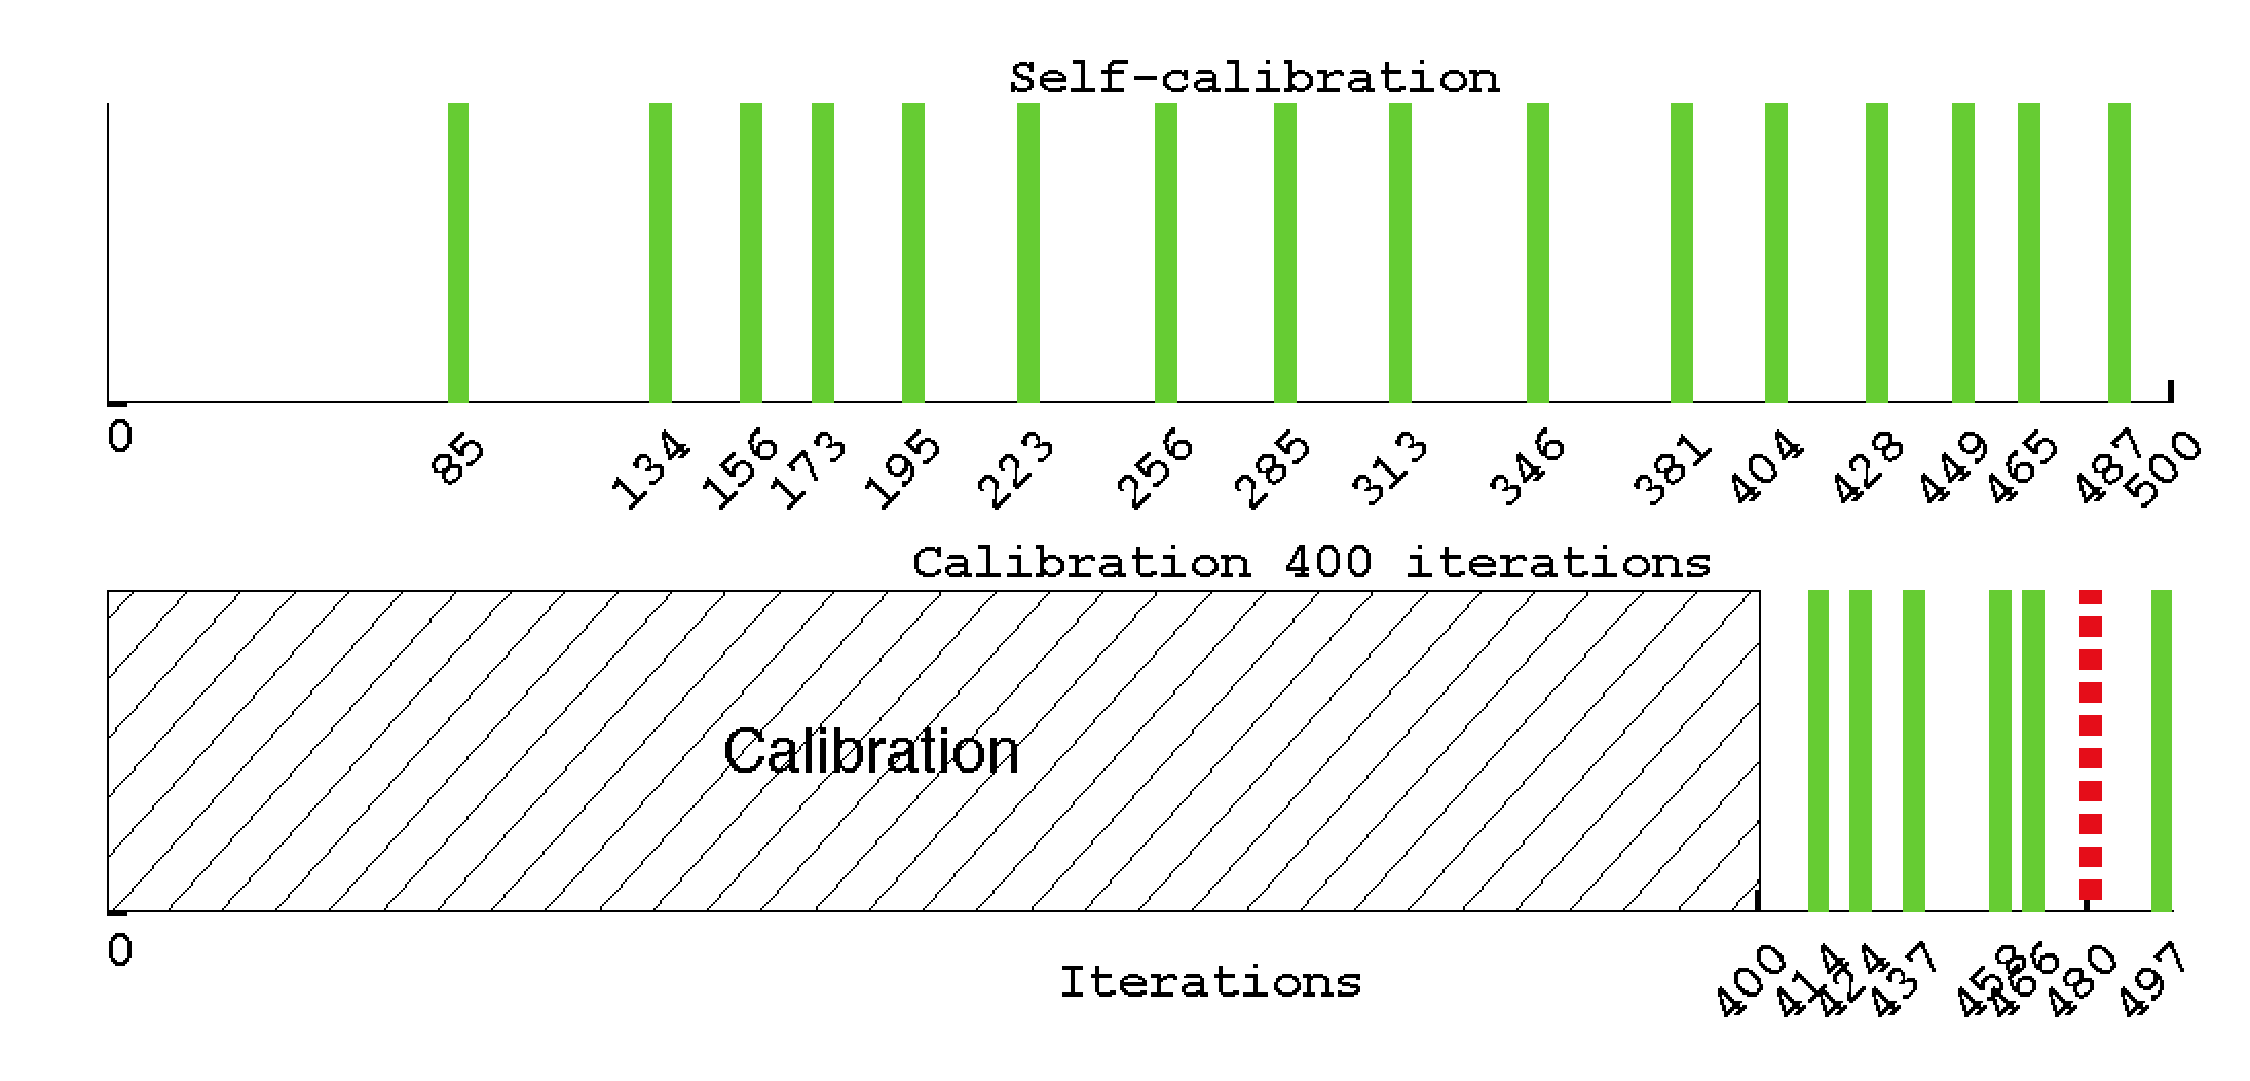
\includegraphics[width=\sequencesize\columnwidth]{\imgpath/plot_the_aaai_sequence.eps}
\caption{Time-line of one run from EEG dataset of $80$ percent ten-fold classification accuracy, self-calibration (top) versus 400 steps calibration (bottom). Green (filled) and red (dashed) bars represents respectively correct and incorrect task achievement. The proposed self-calibration method allow to reach a first task faster than would take a calibration procedure.}
\label{fig:sequence}
\end{figure} 



Figure~\ref{fig:sequence_evolution} shows the evolution of classification rate between our self-calibration method with a calibration procedure of 400 steps. As our method assigns different labels to each new teaching signal, the resulting classifiers have different performances, which help identifying the correct task. Once a task is identified (e.g.\ step 85 and 134), the corresponding labels are taken as ground truth, and all classifiers will have the same accuracies. As the agent starts exploring again to estimate the new tasks, all the classifiers except the true one will start to have worse accuracies again.

\begin{figure}[!ht]
\centering
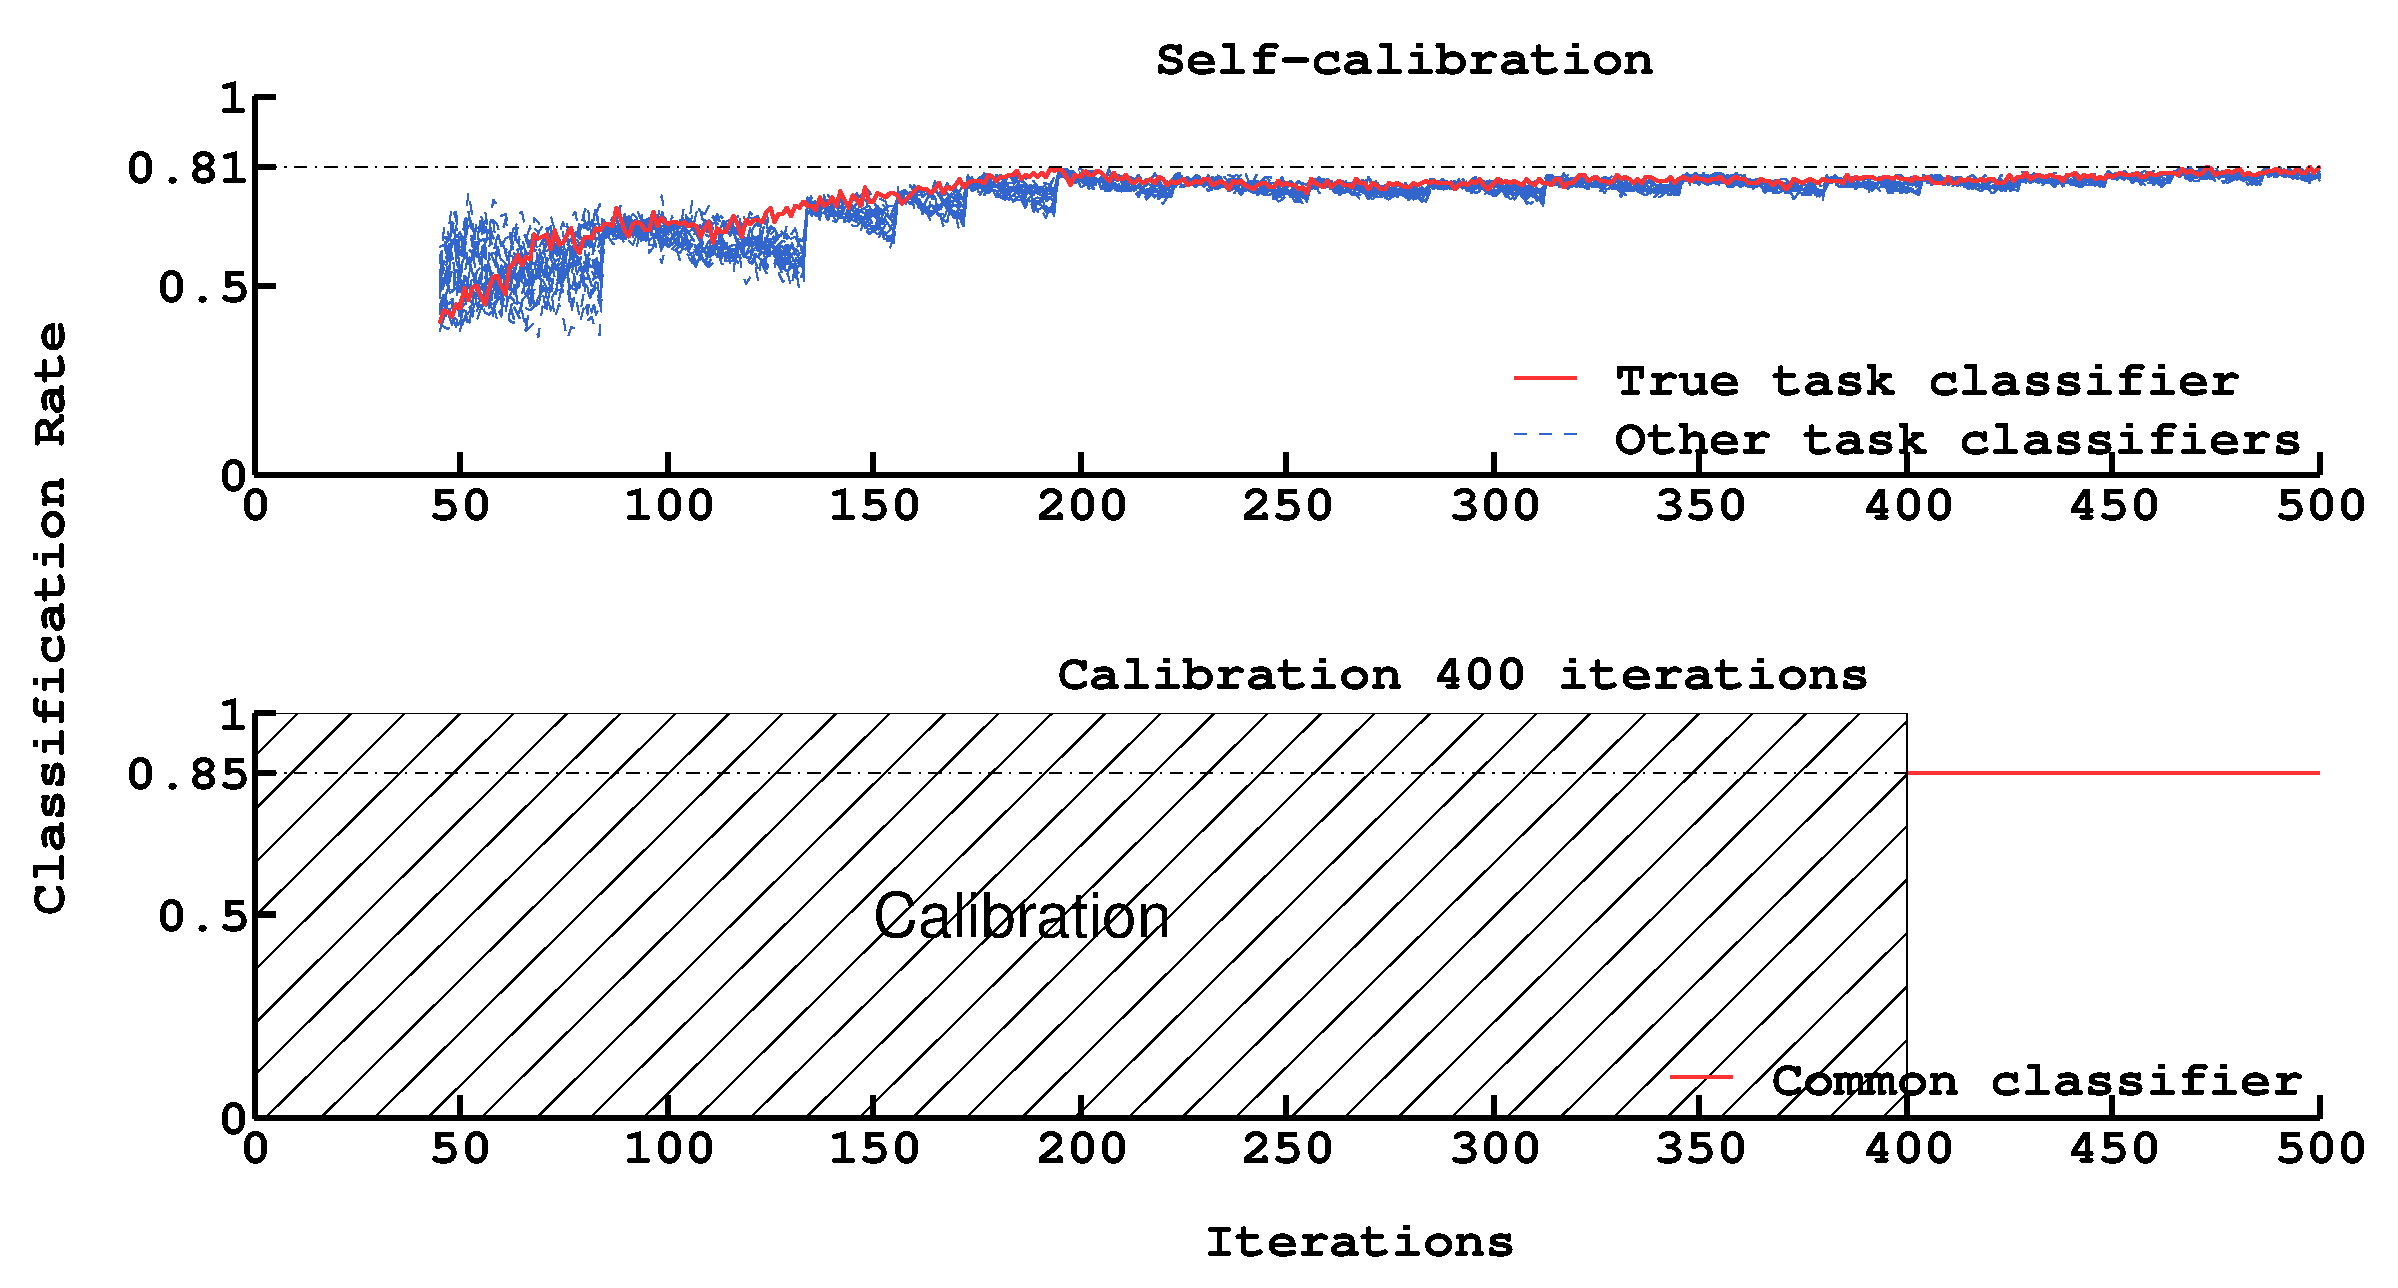
\includegraphics[width=\sequencesize\columnwidth]{\imgpath/plot_evo_classification_rate.eps}
\caption{Evolution of classification rate of one run from EEG data, self-calibration (top) versus 400 steps calibration (bottom). On top, the red line represents the classifier corresponding to the successive tasks taught by the user, the dashed blue lines represent all others tasks. Our method updates classifiers every steps.}
\label{fig:sequence_evolution}
\end{figure} 

\subsection{Planning}

\begin{figure}[!ht]
    \centering
    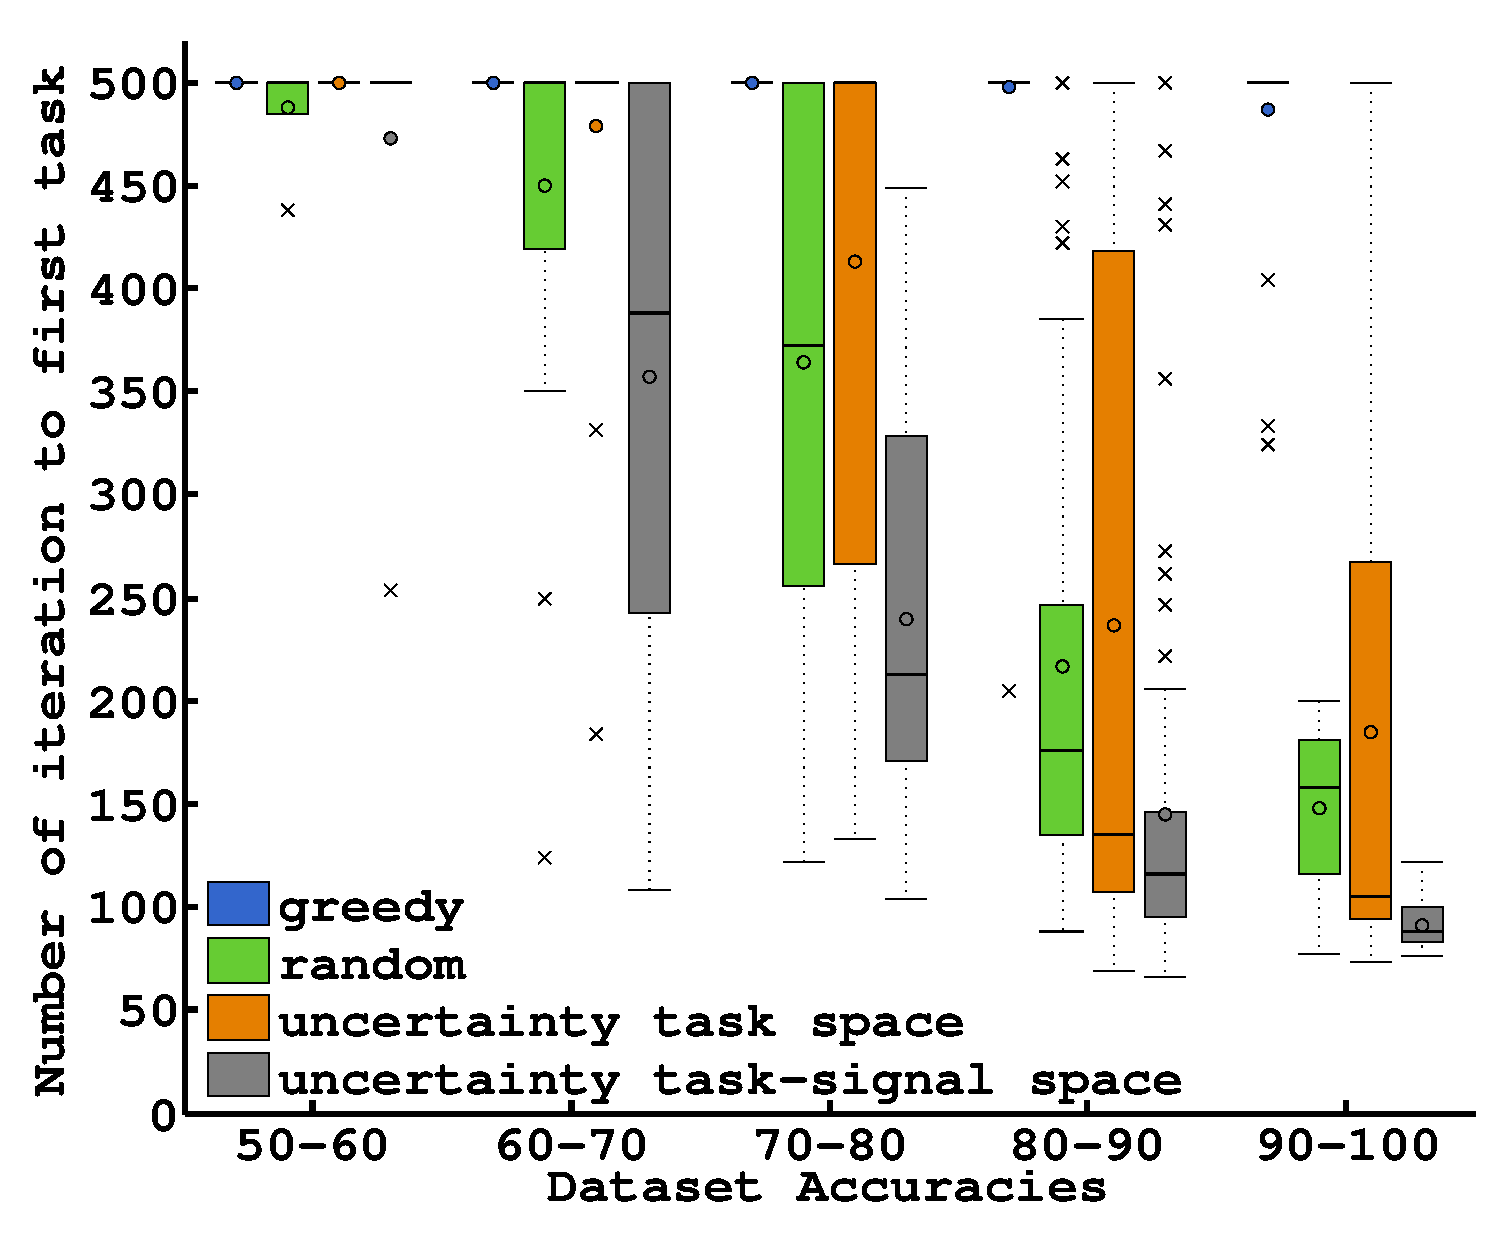
\includegraphics[width=\plotsize\columnwidth]{\imgpath/plot_EEG_planning.eps}
    \caption{Number of steps to complete first task using EEG data of different quality. The EEG data have similar properties than our 30 dimensional simulated data in Figure~\ref{fig:artificialplanning}. Our planning method based on both the task and the signal to meaning mapping uncertainty is more efficient that choosing action randomly, greedily or only based on the uncertainty on the task.}
    \label{fig:planningEEG}
\end{figure}


\subsection{Time to first task}

Figure~\ref{fig:firstEEG} shows the results per group of dataset. Our algorithm allows to complete the first task without errors and in a fair amount of iteration.  For our method, the learning time is strongly correlated with the dataset quality. However calibration methods, which do not update their classifier once calibrated, identify more tasks incorrectly.

\begin{figure}[!ht]
\centering
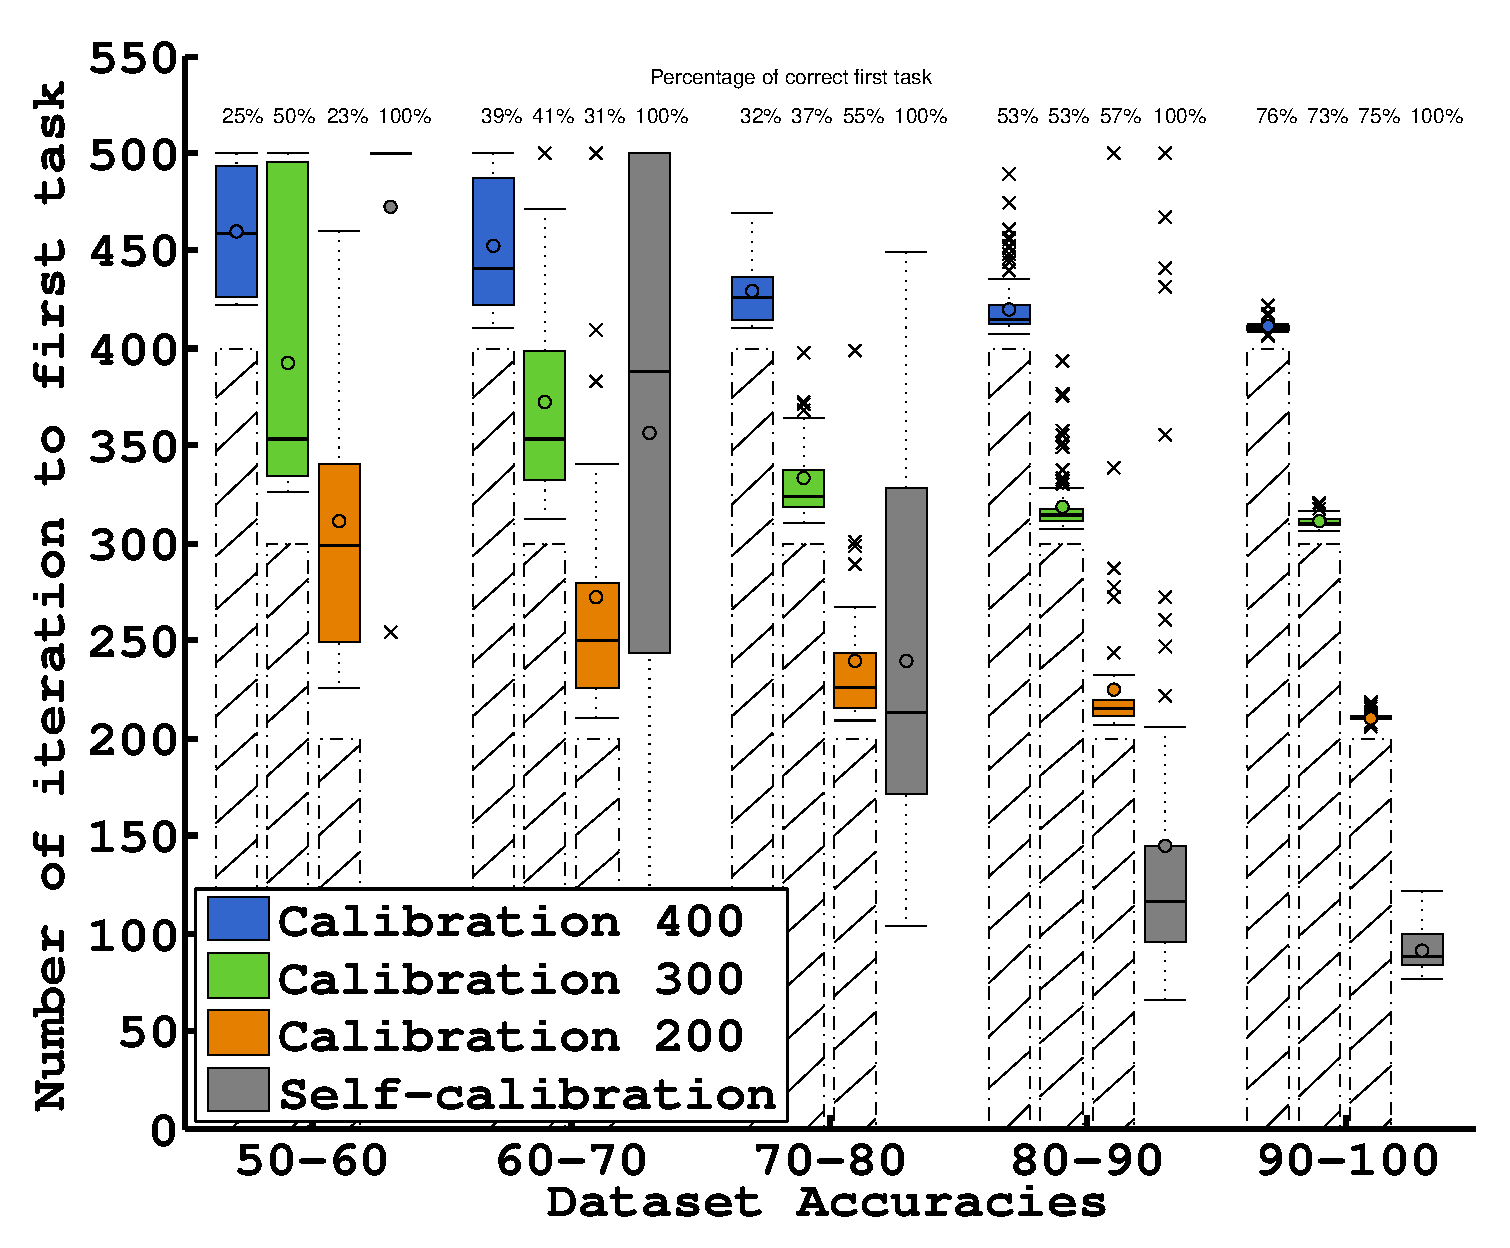
\includegraphics[width=\plotsize\columnwidth]{\imgpath/plot_EEG_calib_firstconf.eps}
\caption{Number of steps to complete first task with EEG data. The percentage of time the task first task was correct is show on top of the each box plot. The method scale well to EEG data. Contrary to the standard calibration approaches, we do not make mistakes with low quality datasets.}
\label{fig:firstEEG}
\end{figure} 

\subsection{Cumulative performances}

Figure~\ref{fig:nCorrectEEG} compares the number of tasks that can be achieved in 500 steps. With 90\% and more dataset quality we can achieve about 20 tasks on average. The results are consistent with artificial dataset analysis.

\begin{figure}[!ht]
\centering
\includegraphics[width=\plotsize\columnwidth]{\imgpath/plot_EEG_calib_nCorrect.eps}
\caption{Number of task correctly achieved in 500 steps with EEG data. Calibration methods can not complete a significant number of task as most of the time is spent on calibration.}
\label{fig:nCorrectEEG}
\end{figure} 

The calibration methods can not complete many task as a significant amount of iteration was used for calibrating the system. A calibration of 200 steps makes as many good estimation than our method, but it also makes many wrong estimation, see Figure~\ref{fig:nWrongEEG}. For calibration methods, the less time spent on calibration, the poorer the classifier which implies more mistakes.

\begin{figure}[!ht]
\centering
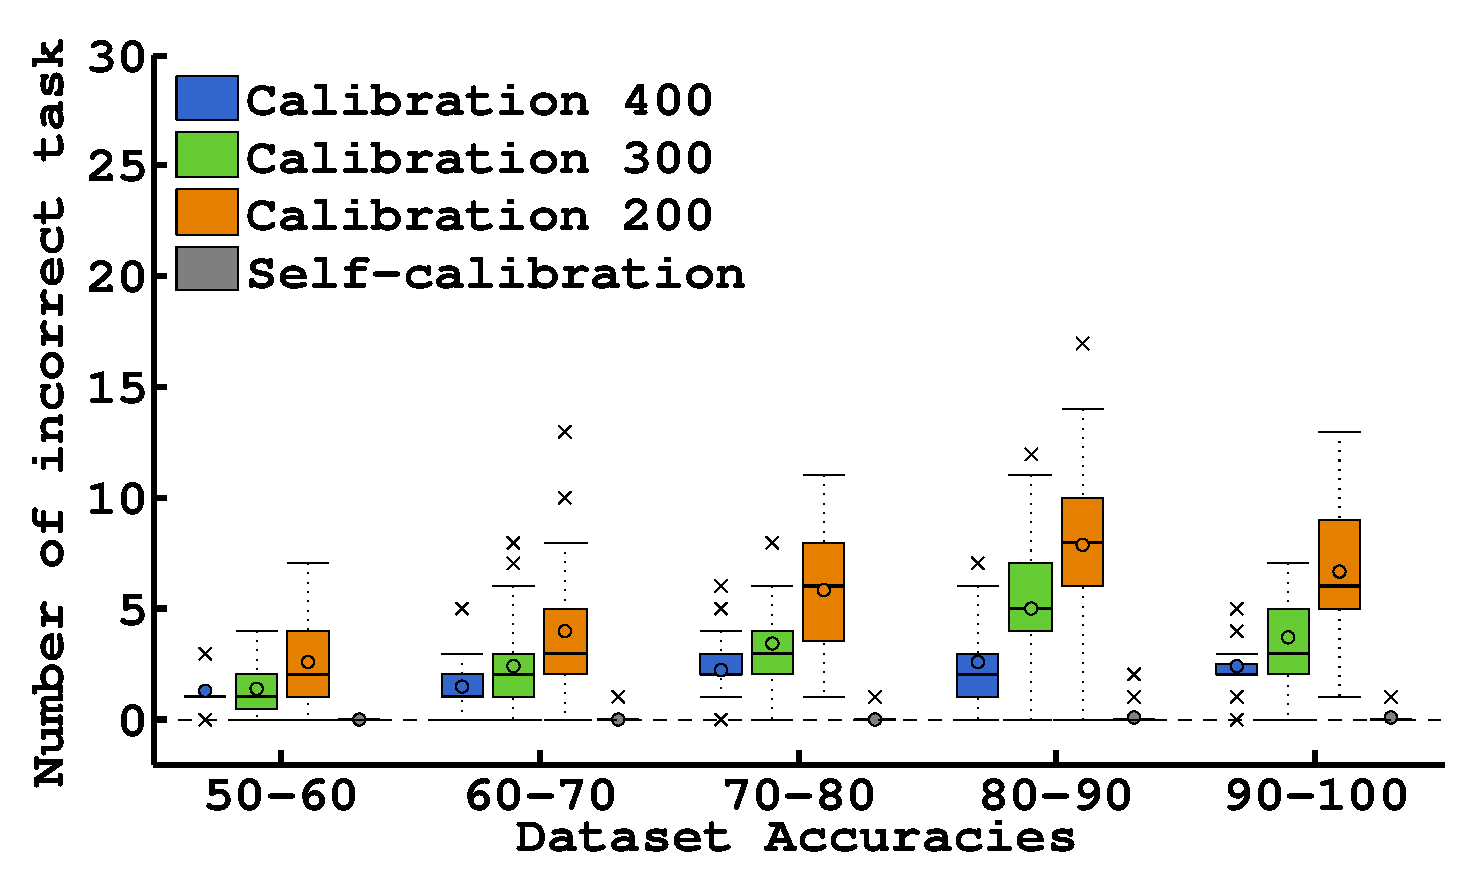
\includegraphics[width=\plotsize\columnwidth]{\imgpath/plot_EEG_calib_nWrong.eps}
\caption{Number of task incorrectly achieved in 500 steps with EEG data. Calibration methods, which do not update their models once calibrated, make more errors.}
\label{fig:nWrongEEG}
\end{figure}

\subsection{Last 100 iterations performances}

Figure~\ref{fig:nCorrectEEG_last100} compares the number of task that can be achieved during the last 100 steps with EEG data. With 80-90\% dataset quality, all methods achieve an average success rate of one task every 20 steps. However calibration methods, which do not update their models once calibrated, make more mistakes (see figure \ref{fig:nWrongEEG_last100}).

\begin{figure}[!ht]
\centering
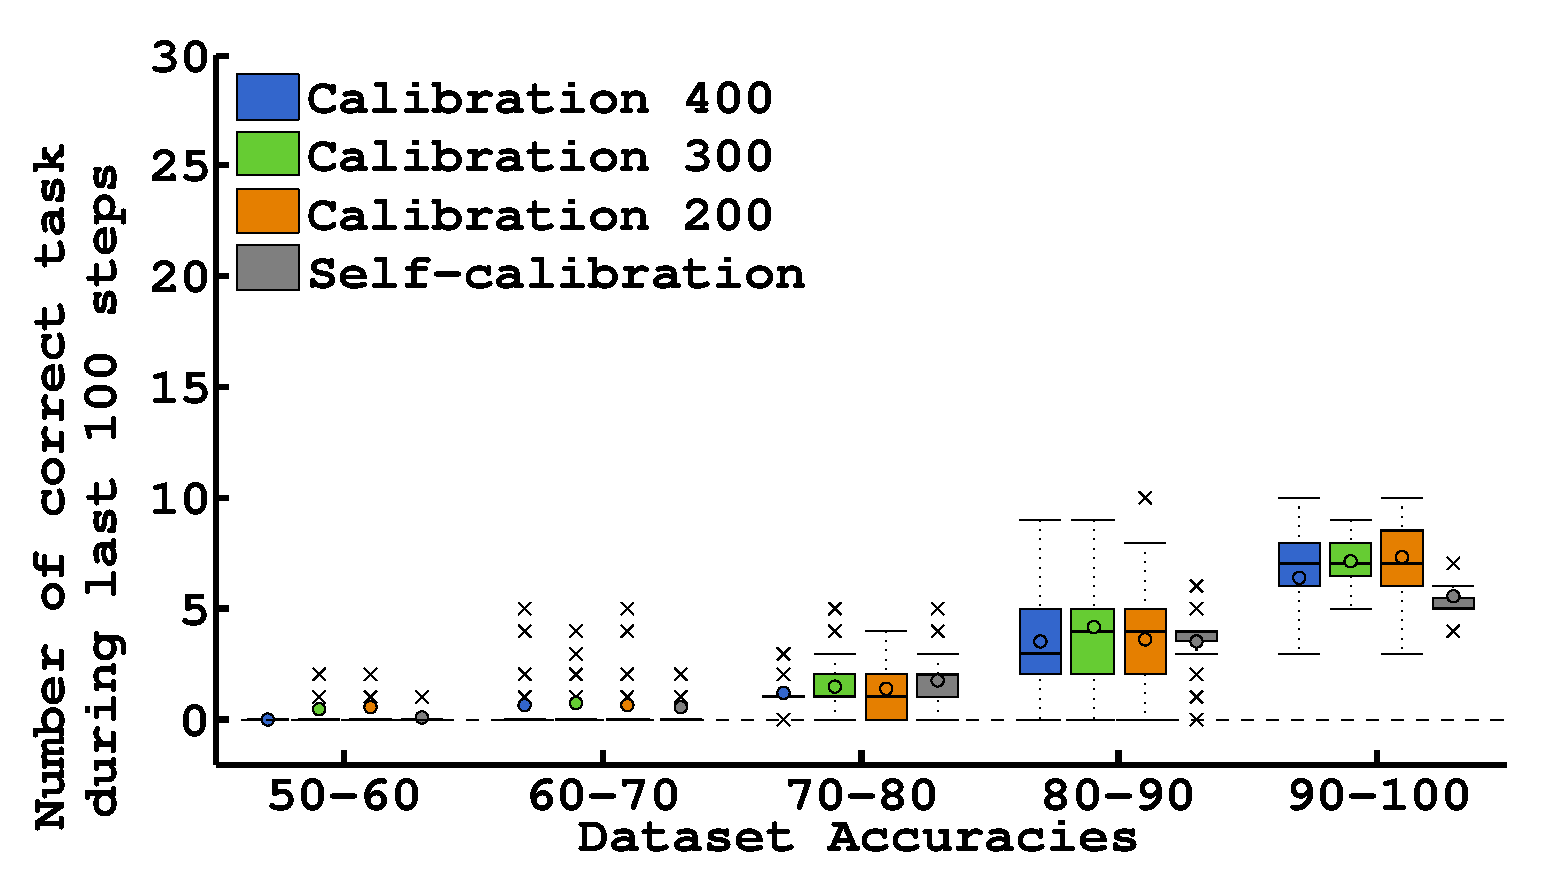
\includegraphics[width=\plotsize\columnwidth]{\imgpath/plot_EEG_calib_nCorrect_last100.eps}
\caption{Number of task correctly achieved during the last 100 steps with EEG data. All methods have equivalent successful reaching rate.}
\label{fig:nCorrectEEG_last100}
\end{figure} 

\begin{figure}[!ht]
\centering
\includegraphics[width=\plotsize\columnwidth]{\imgpath/plot_EEG_calib_nWrong_last100.eps}
\caption{Number of task incorrectly achieved during the last 100 steps with EEG data. Calibration methods, which do not update their models once calibrated, make more errors.}
\label{fig:nWrongEEG_last100}
\end{figure} 

shows the number of tasks identified with respect to the accuracy of the dataset, and the number of tasks incorrectly identified. Notice how the number of identified task is correlated to the quality of the dataset. Importantly, we were able to identify 15 to 20 tasks in 500 steps on good quality dataset without the need for a calibration procedure.


%%%%%%%%%%%%%%%%%%%%%%%%%%%%%%%%%%%%%%%%%%%%%%
%%%%%%%%%%%%%%%%%%%%%%%%%%%%%%%%%%%%%%%%%%%%%%
%%%%%%%%%%%%%%%%%%%%%%%%%%%%%%%%%%%%%%%%%%%%%%
%%%%%%%%%%%%%%%%%%%%%%%%%%%%%%%%%%%%%%%%%%%%%%
%%%%%%%%%%%%%%%%%%%%%%%%%%%%%%%%%%%%%%%%%%%%%%
\section{Why we are cheating with pre-recorder EEG samples}


cite the work of chavariage and inaki which show variabliltiy in the teaching signals due to the task and teachign protocol

We can identify two main differences between our method and the usual calibration procedure for this kind of BCI experiments:
\begin{enumerate}
\item \textbf{Positive/Negative percent ratio of training examples}. Following the literature \cite{chavarriaga2010learning, iturrate2013task} we used a 80/20 percent ratio. Table \ref{tab:correctLabelRatio} shows the positive/negative ratio obtained following our planning method. The ratio we obtain is more balanced, resulting in classifiers with better properties. However a 50/50 percent ratio may lead to practical problems during online real world experiments and should be studied in more details, see open questions in section \ref{sec:conclusion}.
\item \textbf{Online update of multiple classifiers.} Our method integrates new data at every step whose label can differ between task hypothesis. For incorrect task hypothesis, the associated label can be incorrect and decrease the performance of the associated classifier, see figure \ref{fig:planningExplained}c. This dynamic can be observed in figure \ref{fig:sequence_evolution} where classifiers associated to incorrect tasks (in blue) have lower estimated accuracies than the correct one (in red). As a result our algorithm makes different predictions and updates for each hypothesis.
\end{enumerate}

\begin{table}
\centering
\begin{tabular}{c c c}
Dataset Accuracies & Self-calibration & Calibration \\ \hline
50-60 & 0.48 (0.02) & 0.8 (0) \\
60-70 & 0.50 (0.03) & 0.8 (0) \\
70-80 & 0.53 (0.03) & 0.8 (0) \\
80-90 & 0.57 (0.03) & 0.8 (0) \\
90-100 & 0.59 (0.01) & 0.8 (0) \\
\end{tabular}
\caption{Mean ratio of positive examples in training dataset (standard deviation shown in parenthesis). Calibration procedure for ErrP EEG signal usual account for a 80 percent ratio of positive examples. However when following our method we collect as many positive than negative examples. This is likely to impact the quality of Errp signal received from the human during online experiment.}
\label{tab:correctLabelRatio}
\end{table}

\begin{figure}[!ht]
\centering
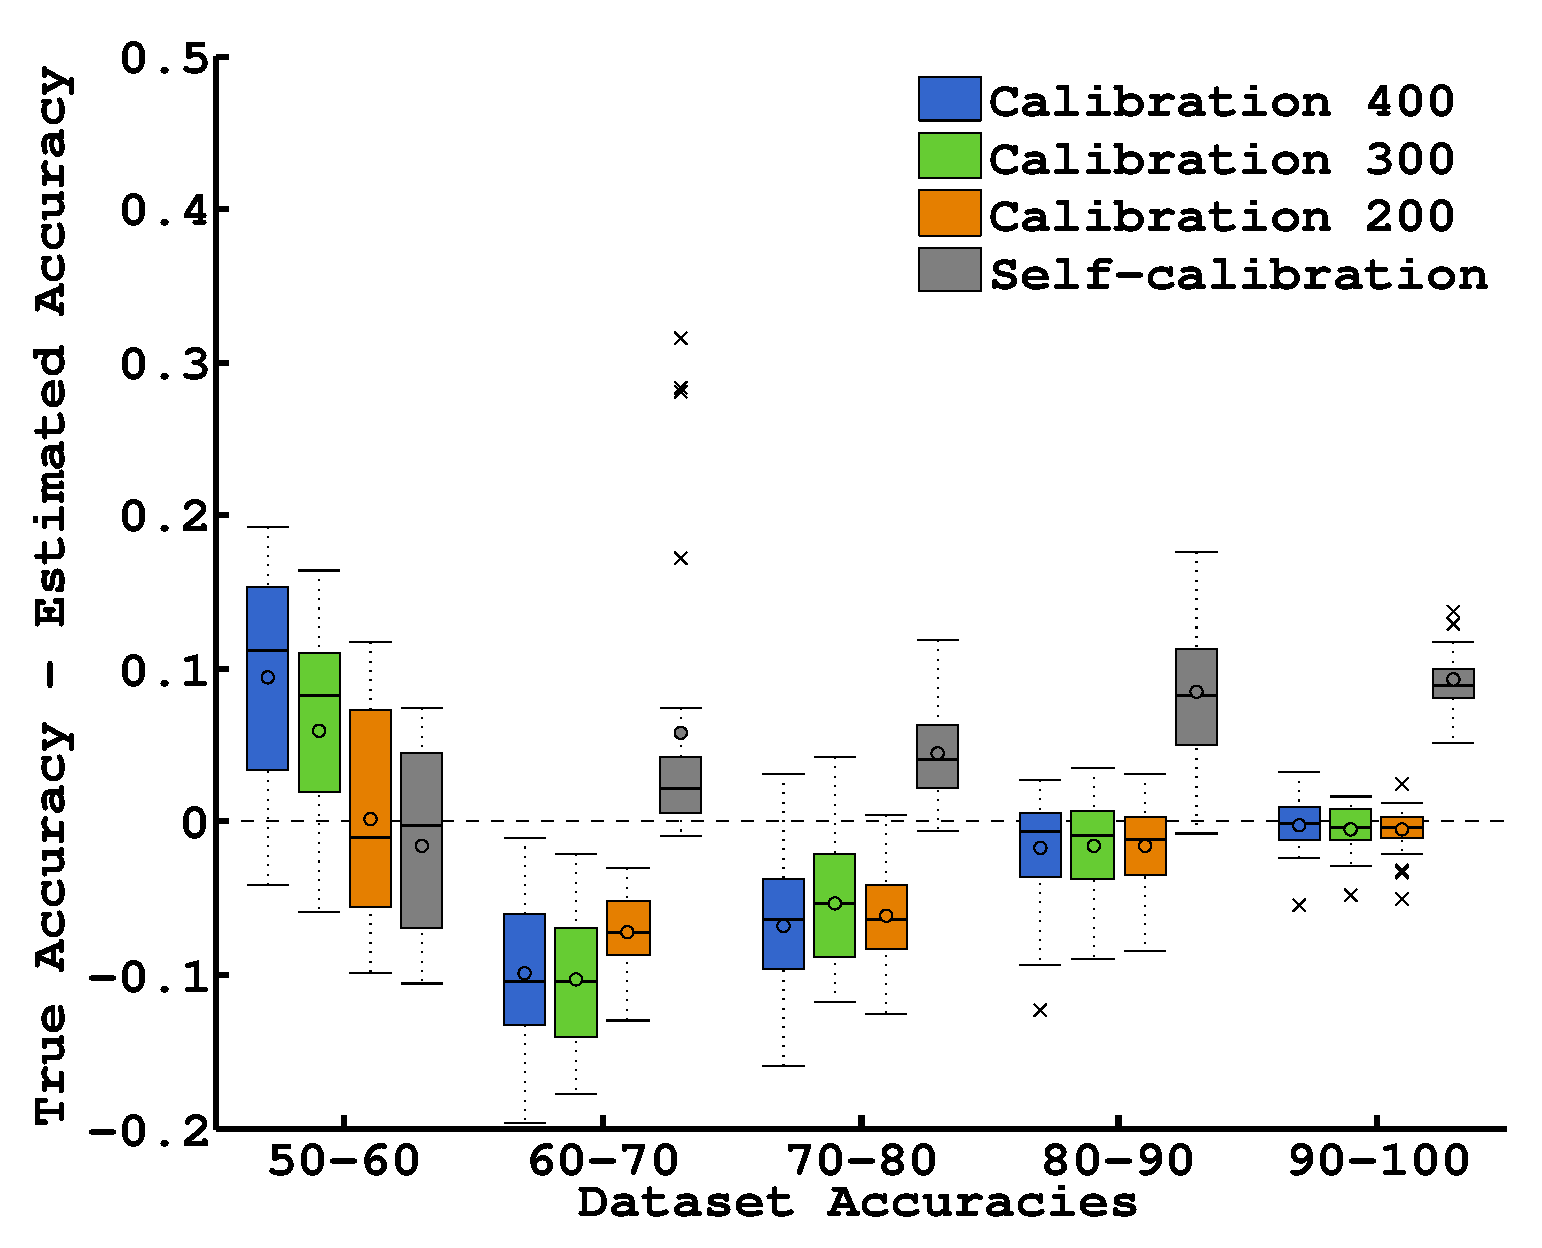
\includegraphics[width=\plotsize\columnwidth]{\imgpath/plot_explaination_for_calib_failure.eps}
\caption{Difference between true accuracy and estimated accuracy. True accuracy is the performance of the classifier on the unused data. Estimated accuracy is the 10 fold cross validation performance of the classifier on collected data. A negative(positive) value indicates the classifier is over(under)-estimating its performance. Calibration methods tend to produce over-confident classifiers, certainly due to the biased positive to negative training example ratio, see table \ref{tab:correctLabelRatio}.}
\label{fig:calibFail}
\end{figure}

%%%%%%%%%%%%%%%%%%%%%%%%%%%%%%%%%%%%%%%%%%%%%%
%%%%%%%%%%%%%%%%%%%%%%%%%%%%%%%%%%%%%%%%%%%%%%
%%%%%%%%%%%%%%%%%%%%%%%%%%%%%%%%%%%%%%%%%%%%%%
%%%%%%%%%%%%%%%%%%%%%%%%%%%%%%%%%%%%%%%%%%%%%%
%%%%%%%%%%%%%%%%%%%%%%%%%%%%%%%%%%%%%%%%%%%%%%
\section{Including Prior Information}

\begin{figure}[!ht]
\centering
\includegraphics[width=\plotsize\columnwidth]{\imgpath/powermatching/timefirst.eps}
\caption{Number of steps to complete first task with EEG data. Comparison between our general method (matching), or using the information that ``incorrect'' signals are more powerful than the ``correct'' (power), or both method combined (power matching). The use of the power information affect the usual performance for the low quality dataset. For datasets of low quality, while the time to first seems more advantageous for the method using the power information, most of the estimated task are erroneous (see Figure~\ref{fig:errorfirst_powermatching}) which makes the use of the power information critical for such low quality data. However those errors occurs for very low quality datasets, which are not the main target of our algorithm. For the datasets of higher quality, the power information allow to slightly speed up the learning compared to our method (matching) which do not rely on known information.}
\label{fig:timefirst_powermatching}
\end{figure} 


\begin{figure}[!ht]
\centering
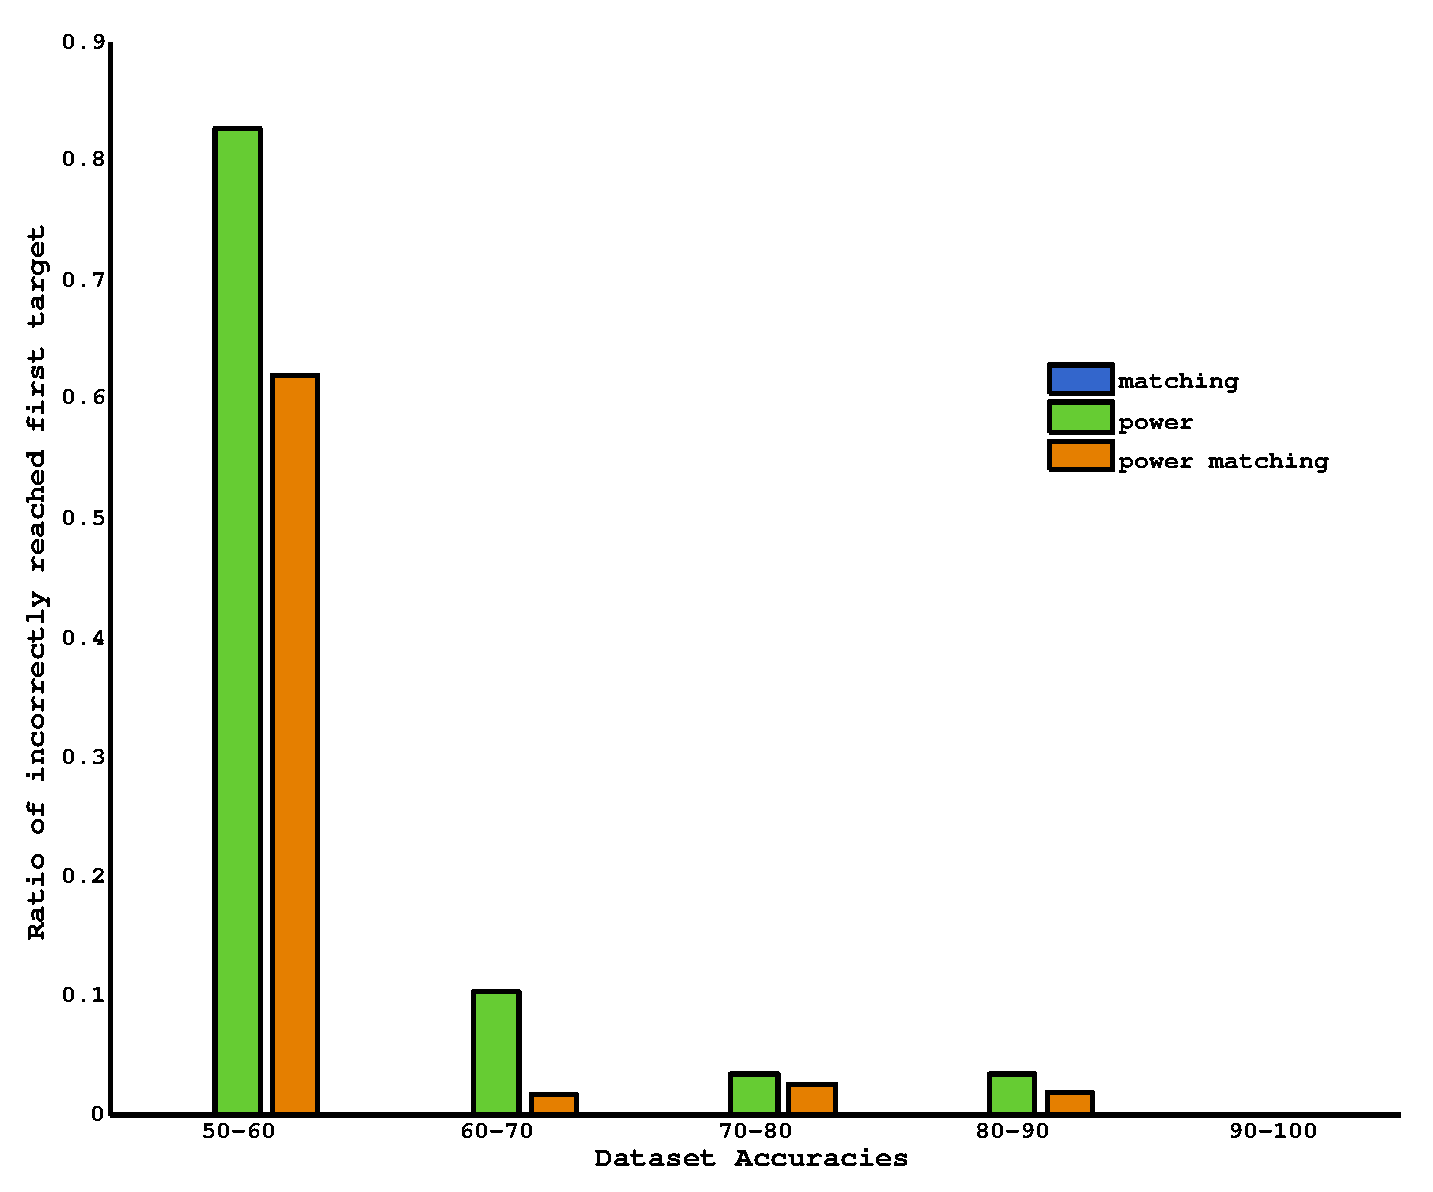
\includegraphics[width=\plotsize\columnwidth]{\imgpath/powermatching/errorfirst.eps}
\caption{Percentage of time the first task estimated was erroneous using EEG data. Comparison between our general method (matching), or using the information that ``incorrect'' signals are more powerful than the ``correct'' (power), or both method combined (power matching). For low quality datasets, the power information increases the number of erroneous estimation. However those errors occurs for very low quality datasets, which are not the main target of our algorithm.}
\label{fig:errorfirst_powermatching}
\end{figure} 


\begin{figure}[!ht]
\centering
\includegraphics[width=\plotsize\columnwidth]{\imgpath/powermatching/correct.eps}
\caption{Number of task correctly achieved in 500 steps with EEG data. Comparison between our general method (matching), or using the information that ``incorrect'' signals are more powerful than the ``correct'' (power), or both method combined (power matching). The power information alone is sufficient to solve our problem but is less efficient than the other methods.}
\label{fig:nCorrect_powermatching}
\end{figure} 

\begin{figure}[!ht]
\centering
\includegraphics[width=\plotsize\columnwidth]{\imgpath/powermatching/error.eps}
\caption{Number of task correctly achieved in 500 steps with EEG data. Comparison between our general method (matching), or using the information that ``incorrect'' signals are more powerful than the ``correct'' (power), or both method combined (power matching). The power information makes more mistakes for low quality dataset which also impact the power matching method. However those errors occurs for very low quality datasets, which are not the main target of our algorithm.}
\label{fig:nWrongEEG_powermatching}
\end{figure} 

For such data it would be better to change the representation of the signal or the classifier used in order to get better .


\begin{figure}[!ht]
\centering
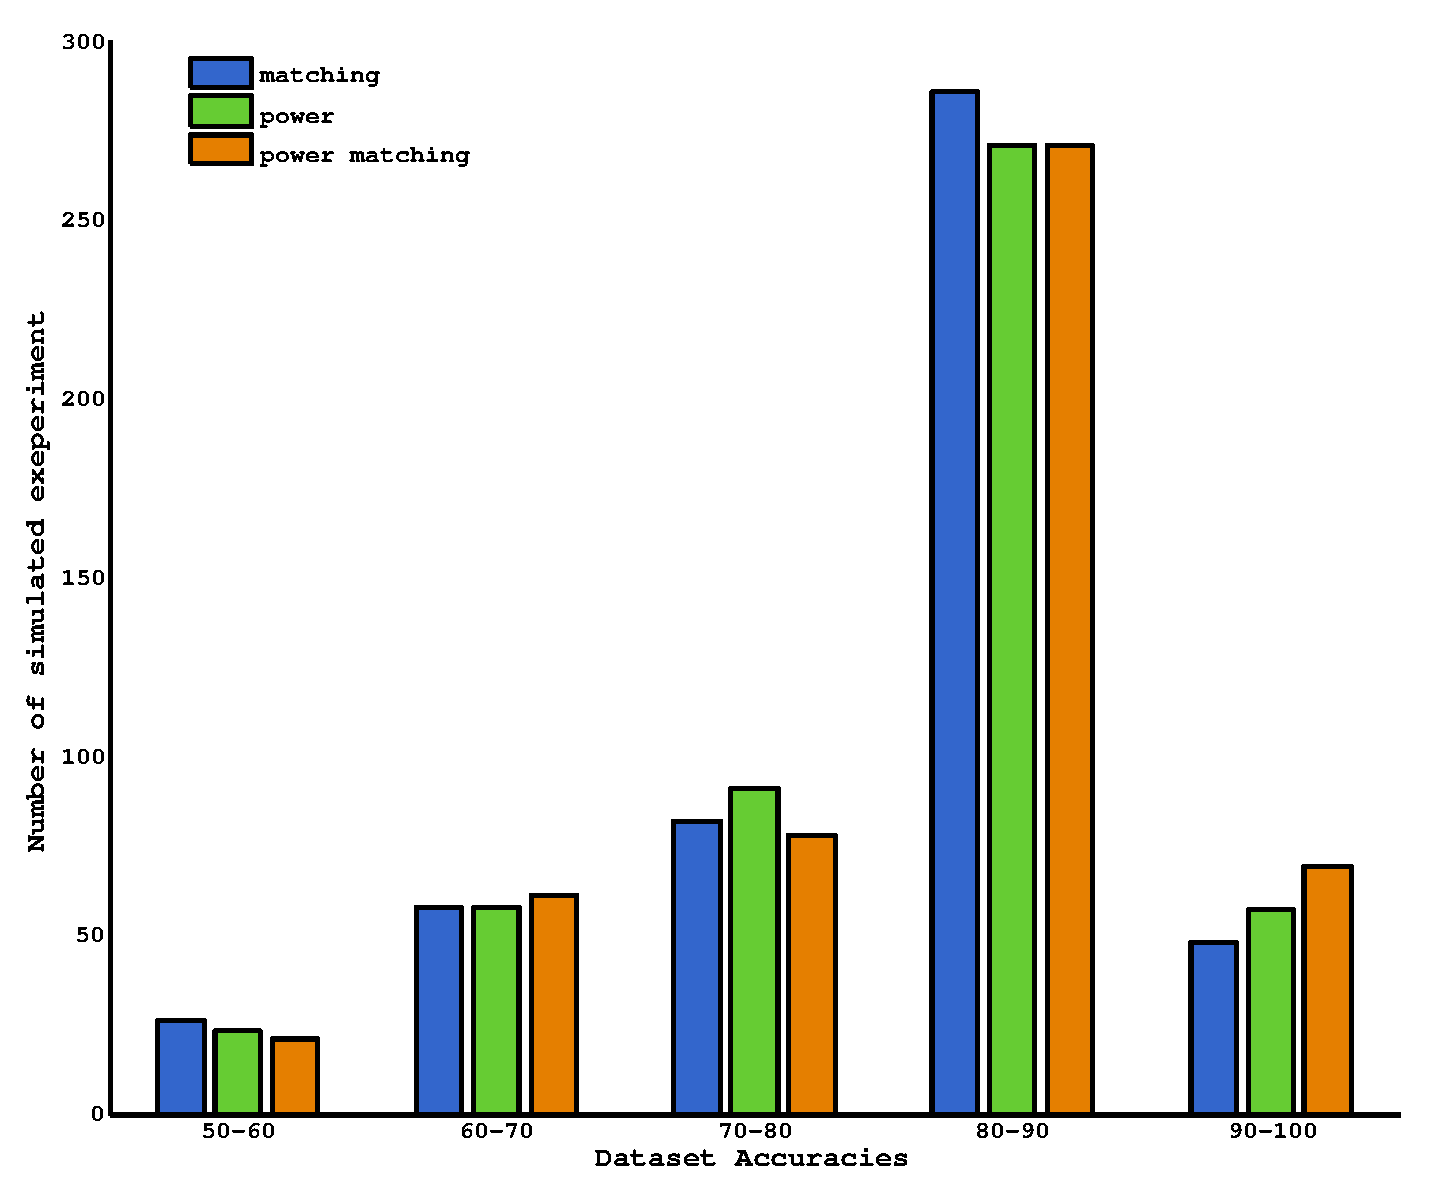
\includegraphics[width=\plotsize\columnwidth]{\imgpath/powermatching/nSim.eps}
\caption{\todo{use a table instead of this figure}}
\label{fig:nSim_powermatching}
\end{figure} 


%%%%%%%%%%%%%%%%%%%%%%%%%%%%%%%%%%%%%%%%%%%%%%
%%%%%%%%%%%%%%%%%%%%%%%%%%%%%%%%%%%%%%%%%%%%%%
%%%%%%%%%%%%%%%%%%%%%%%%%%%%%%%%%%%%%%%%%%%%%%
%%%%%%%%%%%%%%%%%%%%%%%%%%%%%%%%%%%%%%%%%%%%%%
%%%%%%%%%%%%%%%%%%%%%%%%%%%%%%%%%%%%%%%%%%%%%%
\section{Experiments with real users}

\begin{figure}[!ht]
\centering
\includegraphics[width=\plotsize\columnwidth]{\imgpath/onlineXP/timefirst.eps}
\caption{Number of steps to complete first task for all subjects in our online experiments. The results are plotted against the a posteriori computed 10 fold accuracy of our classifier on each subject EEG signals. The relation between data quality and the time to first task is in line with our simulated results shown in Figure~\ref{fig:timefirst_powermatching} Note that this first target was always the correct one for every subject.}
\label{fig:timefirst_online}
\end{figure} 


\begin{figure}[!ht]
\centering
\includegraphics[width=\plotsize\columnwidth]{\imgpath/onlineXP/correct.eps}
\caption{a}
\label{fig:correct_online}
\end{figure} 

\begin{figure}[!ht]
\centering
\includegraphics[width=\plotsize\columnwidth]{\imgpath/onlineXP/error.eps}
\caption{a}
\label{fig:error_online}
\end{figure} 

\todo{summarize all this in a table, but keep two figure to have a visuals which is important.}

\transition

\todo{recap}

Those results with real EEG signals allow us to believe such algorithm could have practical application into the real word. By removing the user of an expert to collect and calibrate the system, we may democratize the use of brain computer interface and allow their users to go out of the labs. However there is number of limitation that would need to be addressed, such as the synchronous interactions assumption, the discrete state, discrete action. Most of the current limitation of this work will be addressed in the next section.

\todo{list limitation here}

% %!TEX root = ../../thesis.tex
\define{\chapterpath}{\allchapterspath/limitations}
\define{\imgpath}{\chapterpath/img}

%
\chapter{Limitations, Extensions and Derivatives}
\label{chapter:limitations}
\minitoc

In the previous chapters, we described an algorithm that allow a robot to learn a new task by interacting with a human partners without defining in advance how the signals of the user maps to the meaning used by the learning agent. We tested this algorithm on two domains, a pick and place scenario using speech commands, and a reaching task scenario using EEG signals. We demonstrated the use of our system online and with real subjects using their brain to assess agent's action with respect to a final desired position.

However a number of assumptions and constraints have been defined. In this chapter we will detail a number of those limitations, discuss the possibility to overcome them and provide small experiments to demonstrate our ideas. 

In section~\ref{chapter:limitiations:simplevsmatching} we compare the performance of Equation~\ref{eq:matchingfilter} and Equation~\ref{eq:matchingfiltercrossvalidation} defined in chapter~\ref{chapter:lfui}. We show that corrrecting the classifier prediction given our knowledge about one classifier (Equation~\ref{eq:matchingfiltercrossvalidation}) makes our algortihm more robust than relying on the raw classifier outputs (Equation~\ref{eq:matchingfilter}).

In section~\ref{chapter:limitations:wordlproperties}, we present preliminary studies on how different properties of the world impacts the efficiency of several planning methods. We specifically study the impact of the size and the maze like properties. This study will highlight the fact that our uncertainty based planning method allow to identify the correct task with best performance in a few types of problems. However we will see that, by not considering the performance on the task itself during the exploration, for some problems our method lacks of efficiency with respect to solving the task as fast as possible.

In section~\ref{chapter:limitations:overlap} we introduce an other method to identify the first target based on models overlap, we present online results with real subjects in a BCI scenario, and show the limitation of this new method to identifying a sequence of multiple tasks.

In section~\ref{chapter:limitations:framegeneric} we insist again on the fact that an interaction frame is not limited to the straightforward meaning correspond we assumed (feedback and guidance), and do not requires the robot to know how to perform a task.

In section~\ref{chapter:limitations:continousstate}, we address the problem of continuous state space, and show that our method is not impacted by the continuous aspect of the problem. Indeed, as our method, when considering a simple frame, only requires to known the policy for each task, we can rely on any algorithm that computes a policy for continuous states given a pre-defined task.

In section~\ref{chapter:limitations:continoushypothesis}, we release the assumption of a finite set of task and rely on a particle filter based method to dynamically update a finite set of hypothesis. We show that sampling actively the new task, as well as selecting actively the next visited state, significantly improves the final performance of our method.

In section~\ref{chapter:limitations:framehypothesis}, we release the assumption that the interaction frame is known and consider the agent as access to a finite number of hypothetic interaction frames. We illustrated this problem in a simple scenario line world scenario. And present results from simulated experiments that demonstrate the ability our method to not only learn the task and the signal to meaning mapping, but also the interaction protocol used by the teacher.

In section~\ref{chapter:limitations:userstudies}, we discuss the need for conducting user studies in more complex domain to evaluate the scalability, efficiency, and acceptability of our method.

In section~\ref{chapter:limitations:proof}, we pinpoint the importance of understanding the properties of our algorithm, and to be able to have some certitude about its convergence and accuracy properties; and we propose a minimalist proof of for our algortihm.

Finally in section~\ref{chapter:limitations:discussion}, we discuss a number of limitations that were not addressed in this work and that are not straightforward to solve given our context. Such as using continuous actions or learning new meanings.

%%%%%%%%%%%%%%%%%%%%%%%%%%%%%%%%%%%%%%%%%%%%%%
%%%%%%%%%%%%%%%%%%%%%%%%%%%%%%%%%%%%%%%%%%%%%%
%%%%%%%%%%%%%%%%%%%%%%%%%%%%%%%%%%%%%%%%%%%%%%
%%%%%%%%%%%%%%%%%%%%%%%%%%%%%%%%%%%%%%%%%%%%%%
%%%%%%%%%%%%%%%%%%%%%%%%%%%%%%%%%%%%%%%%%%%%%%
% %!TEX root = ../../thesis.tex

\section{Why should we temperate classifiers' predictions}
\label{chapter:limitiations:simplevsmatching}

We compare the performance of Equation~\ref{eq:matchingfilter} and Equation~\ref{eq:matchingfiltercrossvalidation} defined in chapter~\ref{chapter:lfui}. The main difference between these two equations is that the second (Equation~\ref{eq:matchingfiltercrossvalidation}) is adding another layer of verification, we temperate the prediction of the classifiers given our knowledge about their quality, which we measure by computing the confusion matrix via a cross-validation procedure.

\subsection{Artificial data}

We consider the same setting as for the experiments described in chapter~\ref{chapter:bci:EEGsignals} and used our two dimensional datasets of different qualities as presented in chapter~\ref{chapter:planning:artificialsignals}. We ran 500 simulations for each method. We consider only the planning method described in chapter~\ref{chapter:planning}.

\paragraph{Time to first task}  Figure~\ref{fig:timefirst_simplevsmatching} compares the number of iterations needed to reach the first task with confidence. We call the method using equation Equation~\ref{eq:matchingfilter} ``simple matching'' and we call ``matching'' the method using Equation~\ref{eq:matchingfiltercrossvalidation} which corrects the classifiers' predictions. There are strong differences between our methods especially for low quality datasets. For extremely overlapping data (50/60\% accuracy), the ``matching'' method is never confident about a task while the ``simple matching'' method show huge variability and sometime outputs confidence after very few time steps. 

\begin{figure}[!htbp]
\centering
\includegraphics[width=\plotsize\columnwidth]{\imgpath/simplevsmatching/timefirst.eps}
\caption{Number of steps to complete the first task using 2D artificial datasets. Comparison between Equation~\ref{eq:matchingfilter} (simple matching) and Equation~\ref{eq:matchingfiltercrossvalidation} (matching), where the latter corrects the predictions of the classifiers given the estimation of their confusion matrix.}
\label{fig:timefirst_simplevsmatching}
\end{figure} 

This over confidence of the ``simple matching'' method reflects in the number of first tasks that were erroneously identified. As shown in Table~\ref{tab:errorTaskRatiosimplevsmatching}, the lower the quality of the data, the higher is the percentage of erroneously identified first task. For extremely overlapping data (50/60\% accuracy), this percentage goes up to 20 percent. While the ``matching'' method may seems too conservative, it is particularly important to not make mistakes when estimating the first task. Indeed once a first task is identified, its associated labels are taken as ground truth. A false estimation of the first task will falsify the signal-label pairs for the remaining of the interaction.

\begin{table}[!htbp]
\centering
\rowcolors{2}{gray!25}{white}
\begin{tabular}{c c c c}
    Dataset Accuracies & Simple Matching &  Matching \\ \hline
    50-60 & 0.21 & 0 \\ 
    60-70 & 0.16 & 0 \\
    70-80 & 0.03 & 0 \\
    80-90 & 0.02 & 0 \\
    90-100 & 0.01 & 0 \\
\end{tabular}
\caption{Percentage of time the estimation of the first task was erroneous using 2D artificial datasets. Comparison between Equation~\ref{eq:matchingfilter} (simple matching) and Equation~\ref{eq:matchingfiltercrossvalidation} (matching), where the latter corrects the predictions of the classifiers given the estimation of their confusion matrix. Only the ``matching'' method, which temperates the predictions of the classifiers, does not make mistakes when estimating the first task.}
\label{tab:errorTaskRatiosimplevsmatching}
\end{table}

\paragraph{Number of tasks achieved in 500 steps}

We compare the number of tasks correctly (Figure~\ref{fig:nCorrect_simplevsmatching}) and incorrectly (Figure~\ref{fig:nWrongEEG_simplevsmatching}) achieved in 500 steps between our two methods. While the ``simple matching'' method allows to reach more targets correctly, it also makes more mistakes for low quality datasets. The ``matching'' method is more conservative and does not make mistakes for all classifier quality, at the cost of reaching fewer targets.

\begin{figure}[!htbp]
\centering
\includegraphics[width=\plotsize\columnwidth]{\imgpath/simplevsmatching/correct.eps}
\caption{Number of tasks correctly achieved in 500 steps using 2 dimensional artificial data. Comparison between Equation~\ref{eq:matchingfilter} (simple matching) and Equation~\ref{eq:matchingfiltercrossvalidation} (matching), where the latter corrects the predictions of the classifiers given the estimation of their confusion matrix. The ``simple matching'' method allows to reach more tasks correctly in 500 steps for all dataset quality.
}
\label{fig:nCorrect_simplevsmatching}
\end{figure} 

\begin{figure}[!htbp]
\centering
\includegraphics[width=\plotsize\columnwidth]{\imgpath/simplevsmatching/error.eps}
\caption{Number of tasks incorrectly achieved in 500 steps using 2 dimensional artificial data. Comparison between Equation~\ref{eq:matchingfilter} (simple matching) and Equation~\ref{eq:matchingfiltercrossvalidation} (matching), where the latter corrects the predictions of the classifiers given the estimation of their confusion matrix. The ``simple matching'' method starts making errors for dataset with accuracies lower than 80 percent. However, the ``matching'' method is more conservative and does not make mistakes.}
\label{fig:nWrongEEG_simplevsmatching}
\end{figure} 

\transition

These results considered only low dimensional dataset (2D), which were generated from Gaussian distribution matching perfectly with the assumption made by our classifiers. We now investigate how the performances are affected by more complex signals, such as the EEG datasets used in chapter~\ref{chapter:bci}, which are 34 dimensional with data distributions that do not necessarily follow the Gaussian assumption.

\subsection{EEG data}

We consider the same setting as for the previous subsection and use the EEG datasets described in chapter~\ref{chapter:bci}. We ran 500 simulations for each method. We consider only the active planning method used in chapter~\ref{chapter:planning}.

\paragraph{Time to first task} Figure~\ref{fig:timefirst_simplevsmatchingEEG} compares the number of iterations needed to reach the first task with confidence. There are strong differences between methods especially for low quality datasets. The ``simple matching'' method performances are not correlated with the classifiers' quality, which reflects the overconfidence of this method.

\begin{figure}[!htbp]
\centering
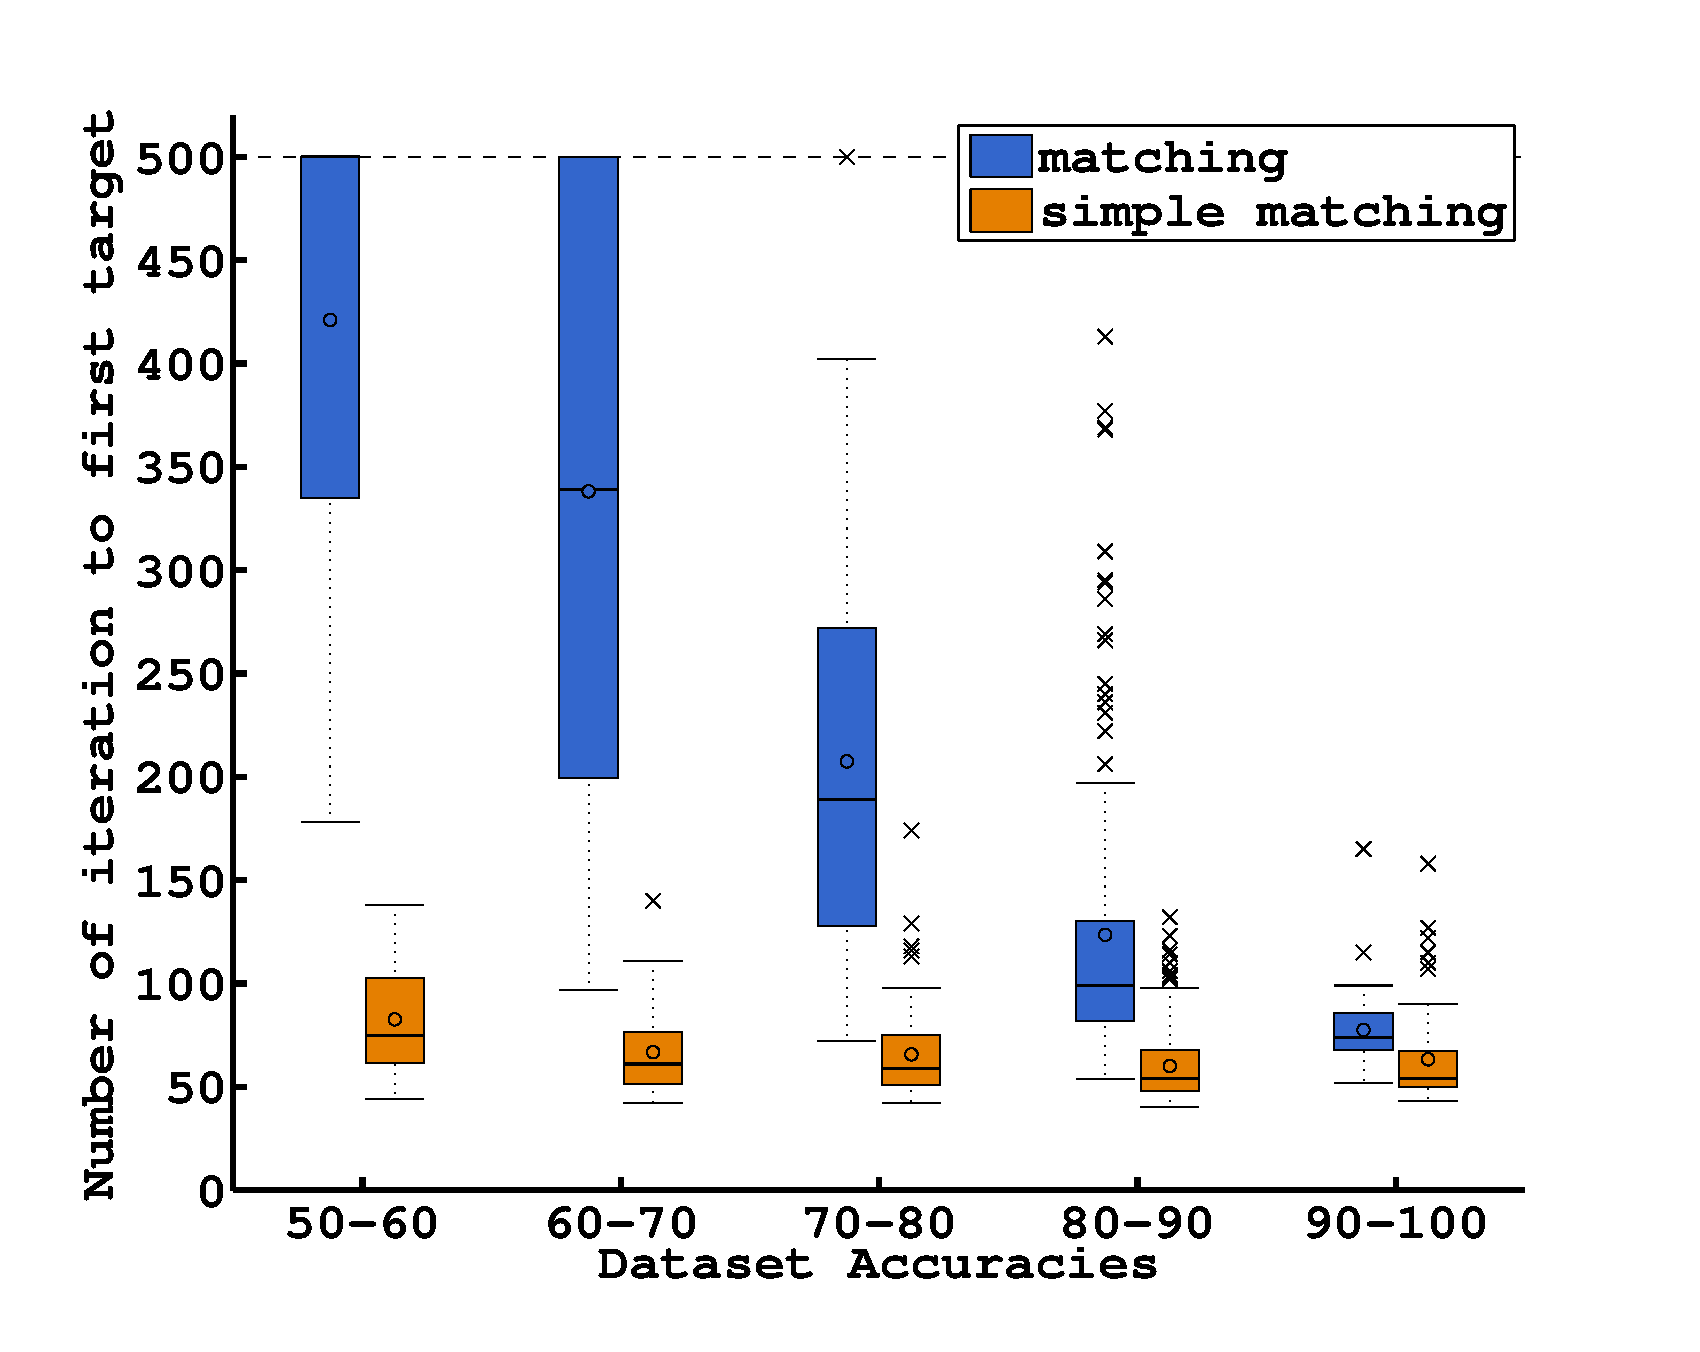
\includegraphics[width=\plotsize\columnwidth]{\imgpath/simplevsmatching/timefirstEEG.eps}
\caption{Number of steps to complete first task with our pre-recorded EEG data. Comparison between Equation~\ref{eq:matchingfilter} (simple matching) and Equation~\ref{eq:matchingfiltercrossvalidation} (matching), where the latter corrects the predictions of the classifiers given the estimation of their confusion matrix. The ``simple matching'' method performances are not correlated with the classifiers' quality, which reflects the overconfidence of this method.}
\label{fig:timefirst_simplevsmatchingEEG}
\end{figure} 

The over confidence of the ``simple matching'' method is reflected by the number of first tasks that were erroneously identified. As shown in Table~\ref{tab:errorTaskRatiosimplevsmatchingEEG}, the lower the quality of the data, the higher the percentage of erroneously identified first tasks. In all cases, this percentage was above 50 percent which makes the use of the ``simple matching'' method impossible for practical experiments. On the contrary, the ``matching'' method does not make any mistake when estimating the first task.

\begin{table}[!htbp]
\centering
\rowcolors{2}{gray!25}{white}
\begin{tabular}{c c c c}
    Dataset Accuracies & Simple Matching &  Matching \\ \hline
    50-60 & 0.81 & 0 \\ 
    60-70 & 0.80 & 0 \\
    70-80 & 0.66 & 0 \\
    80-90 & 0.53 & 0 \\
    90-100 & 0.60 & 0 \\
\end{tabular}
\caption{Percentage of time the first task estimation was erroneous using our pre-recorded EEG data. Comparison between Equation~\ref{eq:matchingfilter} (simple matching) and Equation~\ref{eq:matchingfiltercrossvalidation} (matching), where the latter corrects the predictions of the classifiers given the estimation of their confusion matrix. Only the ``matching'' method, that temperates the predictions of the classifiers does not make mistakes when estimating the first task.}
\label{tab:errorTaskRatiosimplevsmatchingEEG}
\end{table}

\paragraph{Number of tasks achieved in 500 steps}

We compare the number of task correctly (Figure~\ref{fig:nCorrect_simplevsmatchingEEG}) and incorrectly (Figure~\ref{fig:nWrongEEG_simplevsmatchingEEG}) reached in 500 steps. While the two methods allow to reach a similar number of targets correctly. The ``simple matching'' method also makes a many mistakes for all datasets. The ``matching'' method makes only few mistakes for all classifiers' quality.

\visuopti{\newpage}

\begin{figure}[!htbp]
\centering
\includegraphics[width=\plotsize\columnwidth]{\imgpath/simplevsmatching/correctEEG.eps}
\caption{Number of tasks correctly achieved in 500 steps using our pre-recorded EEG data. Comparison between Equation~\ref{eq:matchingfilter} (simple matching) and Equation~\ref{eq:matchingfiltercrossvalidation} (matching), where the latter corrects the predictions of the classifiers given the estimation of their confusion matrix. Both methods reach a similar number of targets correctly when using EEG datasets. The ``simple matching''  method shows more variability.}
\label{fig:nCorrect_simplevsmatchingEEG}
\end{figure} 

\begin{figure}[!htbp]
\centering
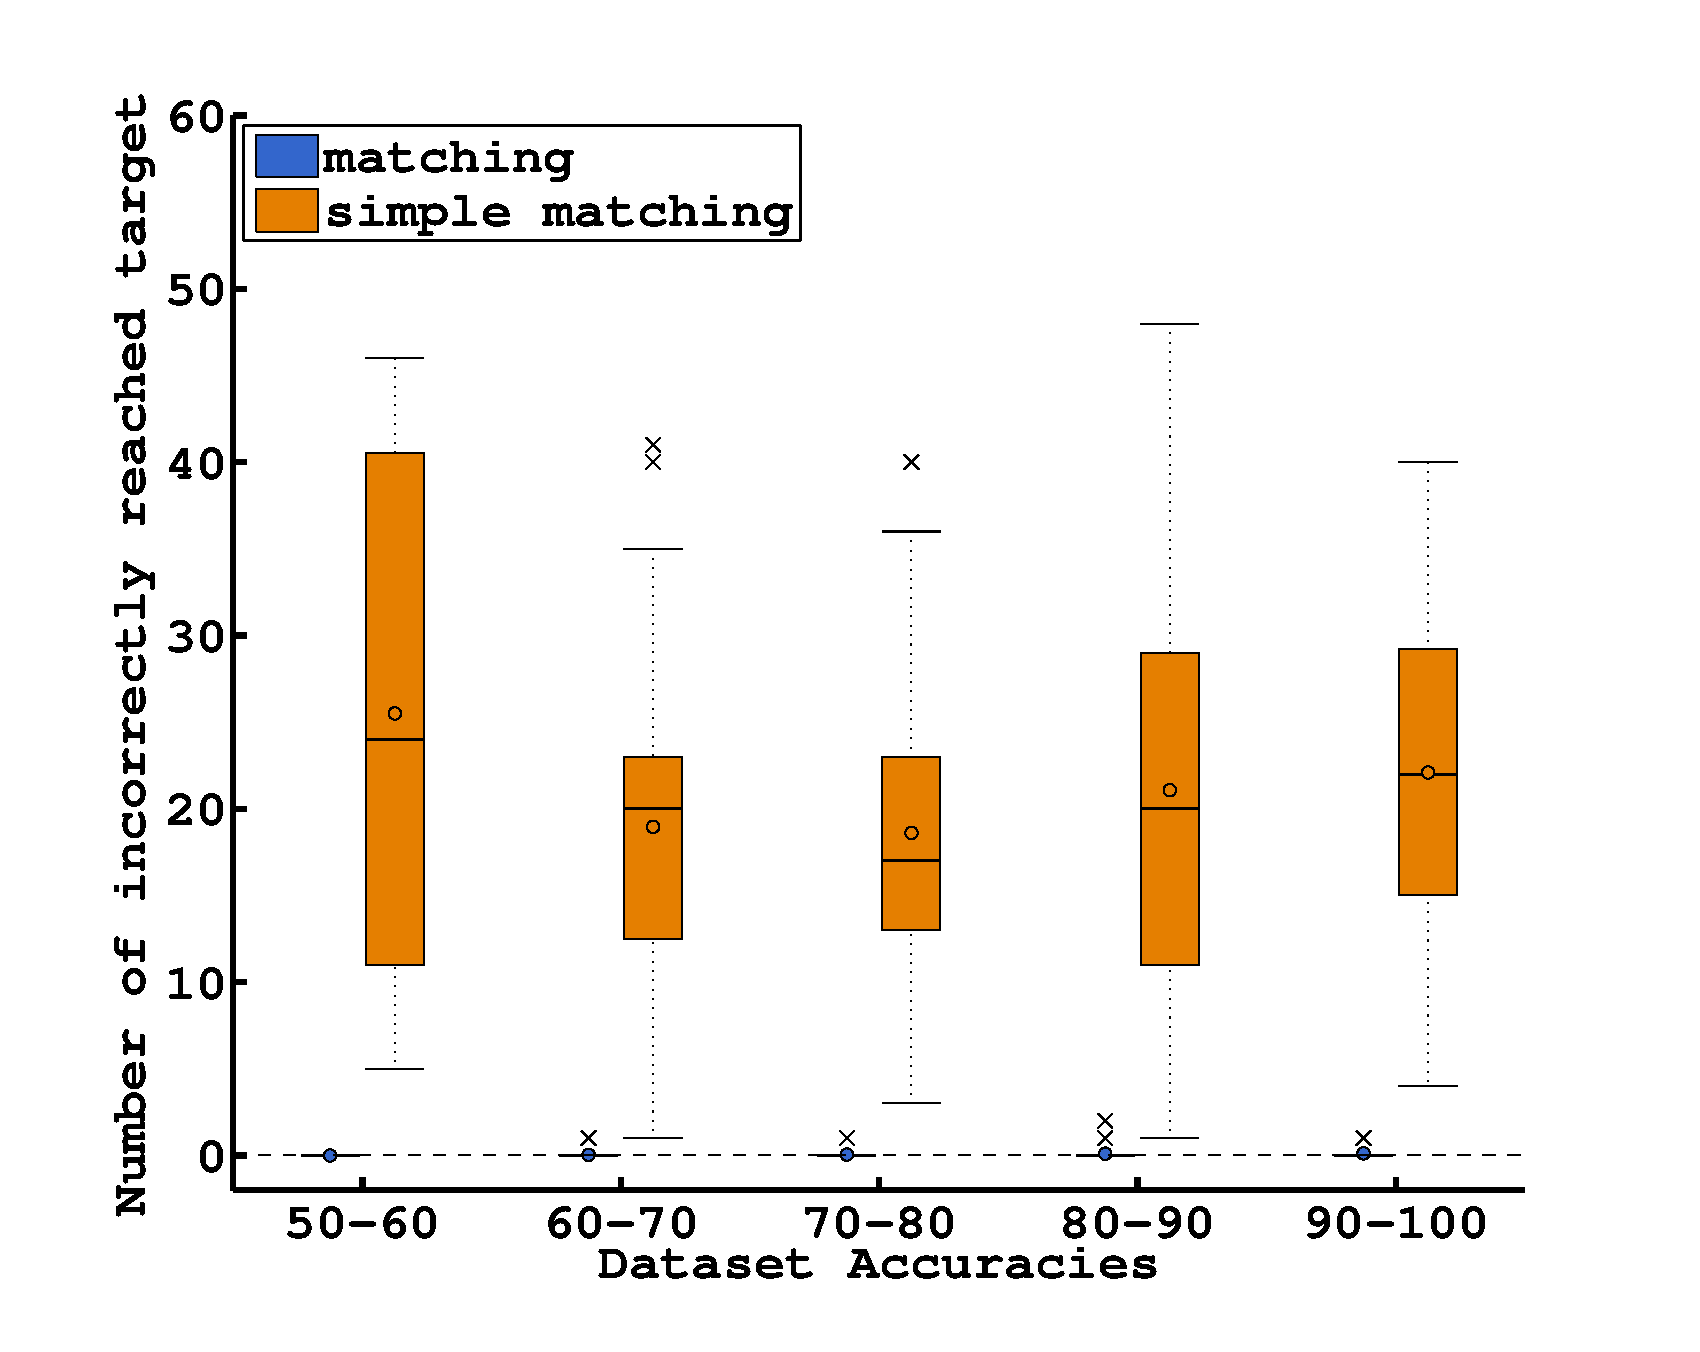
\includegraphics[width=\plotsize\columnwidth]{\imgpath/simplevsmatching/errorEEG.eps}
\caption{Number of tasks incorrectly achieved in 500 steps with our pre-recorded EEG data. Comparison between Equation~\ref{eq:matchingfilter} (simple matching) and Equation~\ref{eq:matchingfiltercrossvalidation} (matching), where the latter corrects the predictions of the classifiers given the estimation of their confusion matrix. The ``simple matching'' is not reliable for EEG data.}
\label{fig:nWrongEEG_simplevsmatchingEEG}
\end{figure} 

\subsection{Discussion}

The results presented in this section confirm that taking into account the uncertainty about the predictions of the classifiers makes the algorithm more robust. However, if we knew the data will be of good enough quality, it is not necessary to correct the classifiers' outputs (as we did for the speech dataset used in chapter~\ref{chapter:lfui}), which divides the computational cost by a factor of 10 (for a 10 fold cross-validation). However, as soon as we have to deal with signals of various qualities and with different properties (like for BCI data in chapter~\ref{chapter:bci}), it is better to include a measure of classification uncertainty in our likelihood update rule.

% %!TEX root = ../../thesis.tex

\section{World properties}
\label{chapter:limitations:wordlproperties}

\question{How the world properties (symmetries, size, \ldots) affect the learning properties?}

As discussed in section~\ref{chapter:lfui:symmetries}, the properties of the world can affect the learning performances. For example some worlds have symmetric properties which makes some tasks impossible to differentiate.

In this section, we compare how various planning methods perform on two different worlds, namely the pick and place scenario and the grid world. We investigate the performance of planning using a random strategy, several $\epsilon$-greedy methods, a strategy based on the task uncertainty (where we do not take the signal to meaning mapping uncertainty in to account), and our uncertainty based method described in chapter\ref{chapter:planning}. We will see that the size of the worlds and the properties of optimal policies impact the performance of these planning methods.

\subsection{Hypothesis and world properties}

We hypothesized that differences in the properties of each world will impact the performances of several planning methods, especially the random method and the e-greedy methods which are blind to the problem properties.

In the coming analysis, we consider three different world instances, a 5 by 5 grid world, a 25 by 25 grid world and the pick and place world of chapter~\ref{chapter:lfui}. In the following we present the main differences between these worlds.

First testing our planning method on a 5x5 and 25x25 allows to test how the size of the world influence the performances and to verify that our uncertainty measure is robust to such change. The main hypothesis is that the random action selection method will not scale well to this change in dimensionality. Indeed, in a 5x5 grid, taking random actions allows to explore the state space quite uniformly in a small number of steps, however in a 25x25 grid (625 states) the robot is unlikely to visit useful states given a limited number of iterations.

We choose to use a 25x25 grid because the resulting number of states (625) is almost equal to the number of states of the pick and place scenario (624), which allows to remove the size effects when comparing those two scenarios. By comparing the grid world and the pick and place scenario, we aim at investing how the maze like properties of the pick and place world compares with the more simple structure of the grid world. For the pick and place scenario, to reach the correct cubes' configuration the robot must achieve a very specific sequence of action in the correct order. As for a maze, only one correct path can be followed, however for the grid world a multitude of path can be chosen.

\todo{The ``maze like'' property can be measure by the amount of overlap between the optimal policies associated to two ``close'' task. For the pick and place scenario, if the signal to meaning mapping were known, to differentiate between two cube configuration that are close together, the agent must go towards those configuration to be able to discard one or an other task. For example, in our illustration of Figure~\ref{fig:lfui:pickplacesequence}, to differentiate between the two first state, one as to reach one of those two states to tell the identify the correct one. Indeed, their corresponding optimal policies are similar for every state except their two final states, i.e. both tasks share the same policies for 622 states our of 624. However for the grid world scenario, if the signal to meaning mapping were known, one could differentiate between the top right state and the state directly on the left of that top right state by simply performing a left action on the bottom right state. And this whatever the size of the grid. The optimal policies of those two task differs for all states along the two columns on the left of the grid, i.e. both tasks share the same policies for only 575 states our of 625 in our 25x25 grid world.}

\subsection{Method}

We used the same conditions as used in chapter~\ref{chapter:planning}, where the teacher is providing instructions following the feedback frame but we use only two dimensional signals of very good quality (i.e. between 90 and 100 percent of classification rate).

We simulated 50 runs of 100 iterations for each planning methods and each world considered. There where 10 steps of initialization before the agent starts computing the first likelihood. During the first 10 steps, the agent where acting randomly for all methods.

\subsection{Results}

In this subsection, we analyze the Figure~\ref{fig:wordlpropertiestimefirst} which displays the number of iterations needed to reach the first task with confidence. We first comment the difference between the 5x5 grid world and the 25x25 grid world, and then compare the grid world and the pick and place scenario.

\begin{figure}[!htbp]
\centering
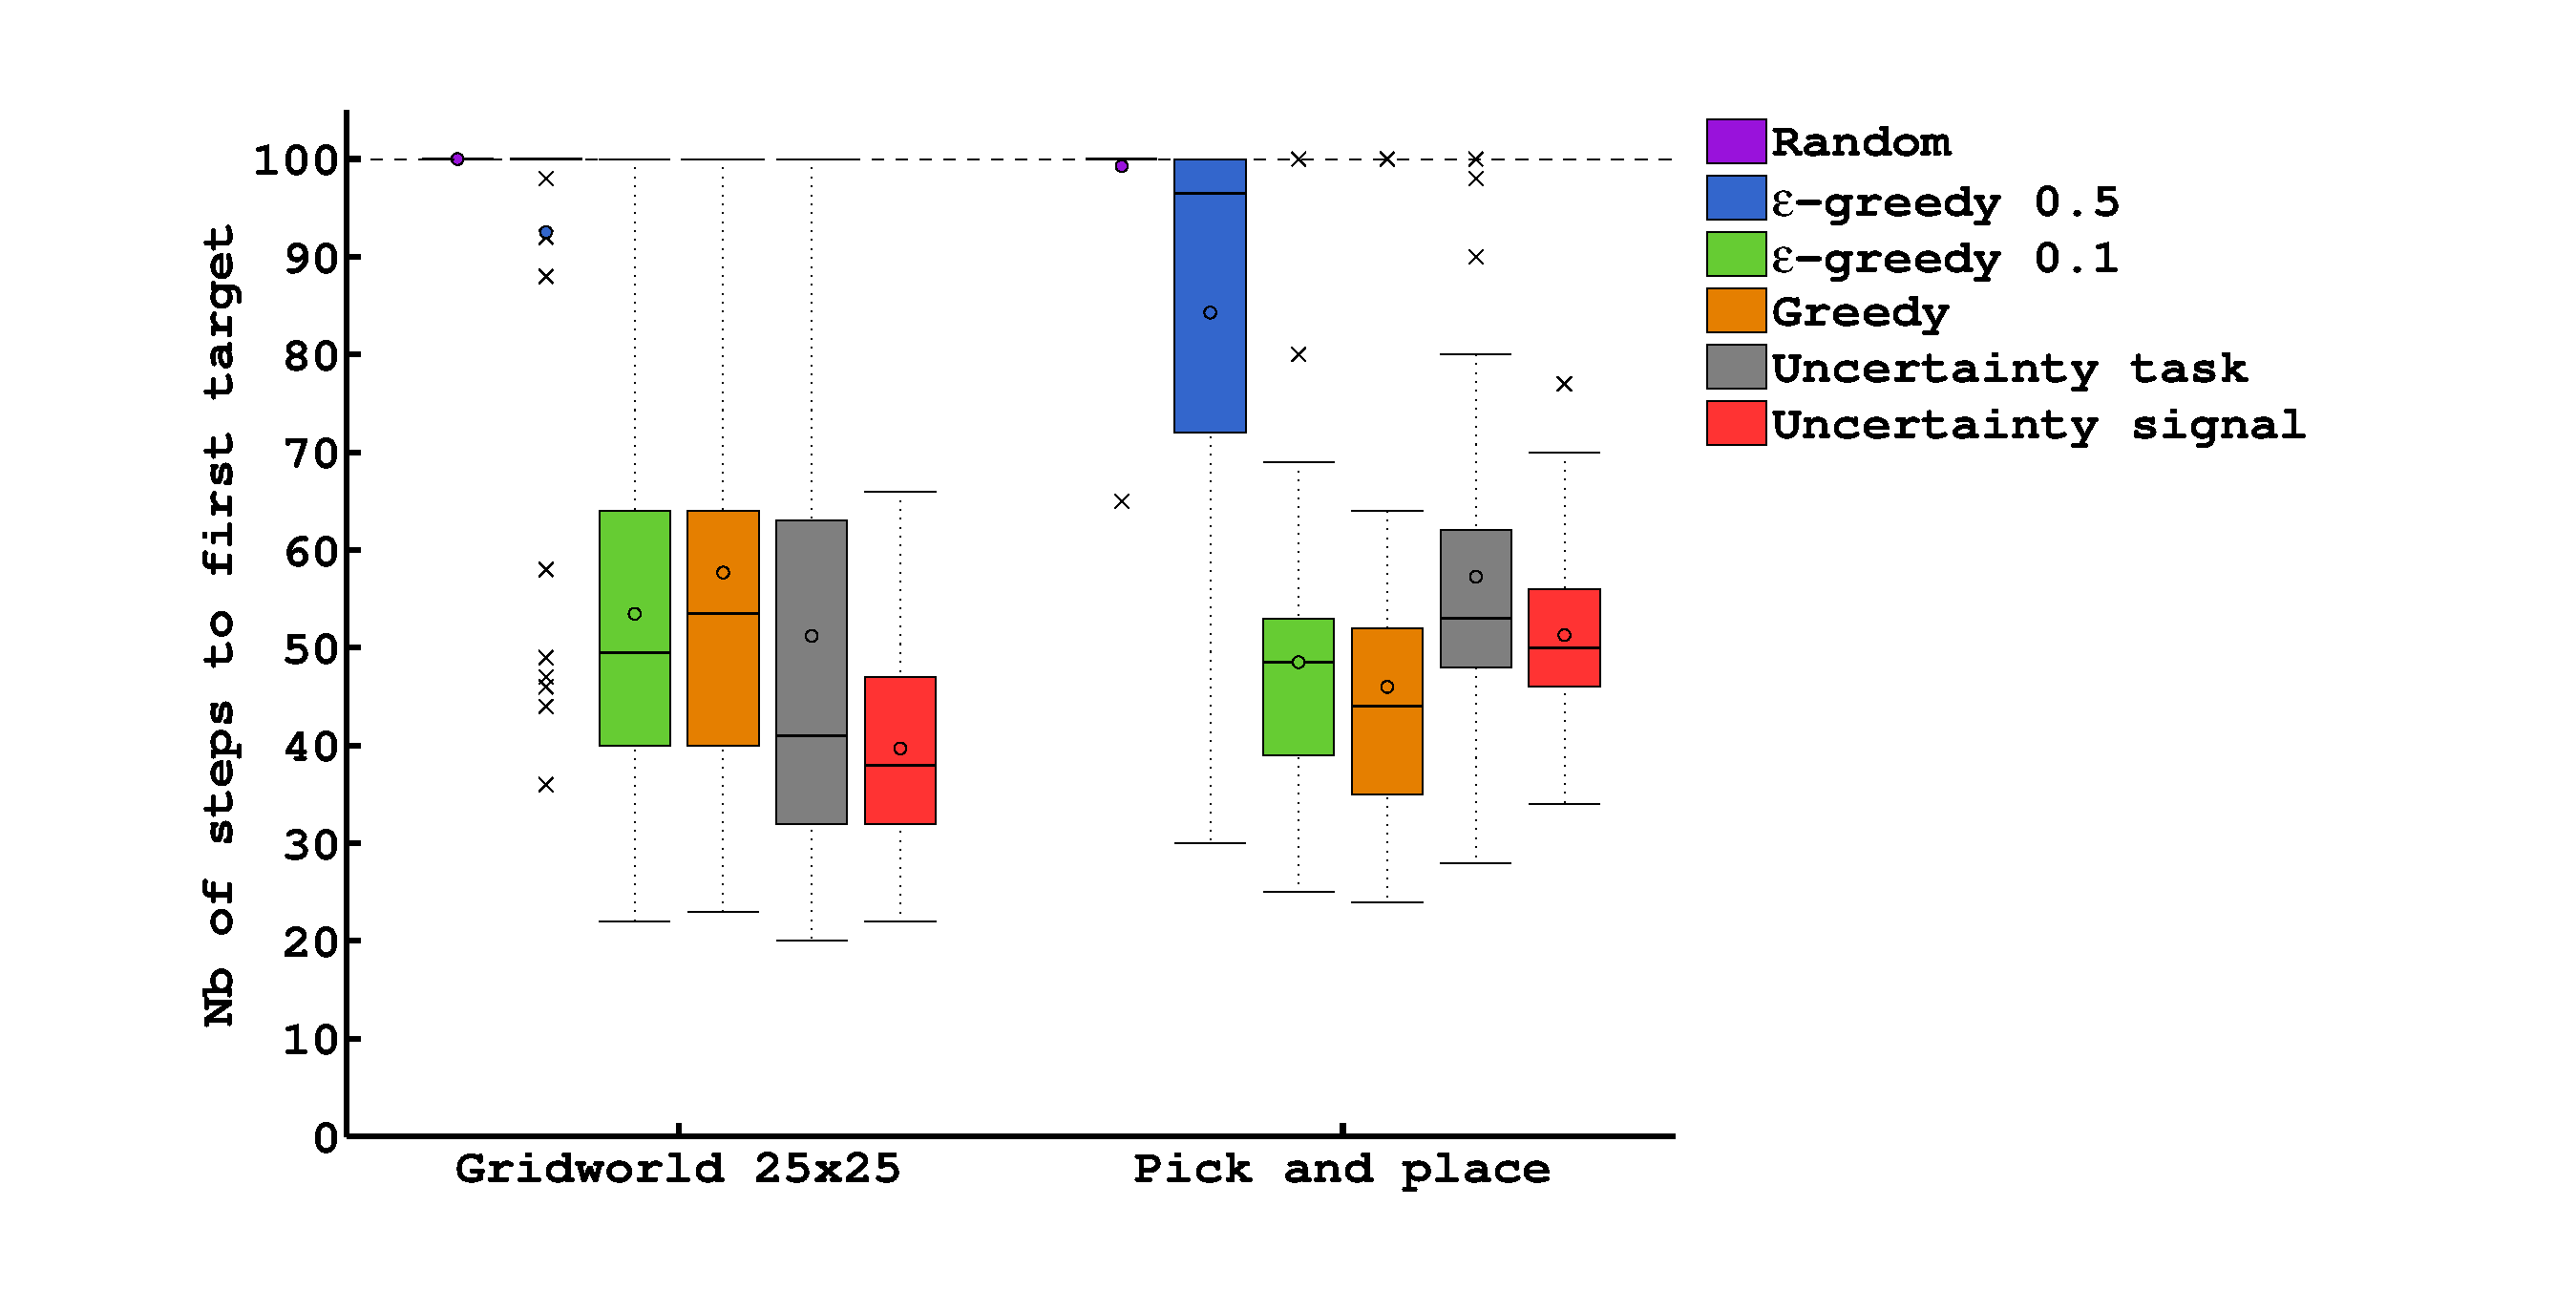
\includegraphics[width=\legendsidesize\columnwidth]{\imgpath/world_properties/firstreach.eps}
\caption{Number of steps needed to reach the first target state with confidence. When the dimensionality of the world increase, selecting actions randomly does not allow to identify any task in 100 iterations. Our uncertainty based method (uncertainty signal), is the most efficient at reaching the first task in the grid world scenarios but seems outperformed by a simple greedy approach in the pick and place scenario.}
\label{fig:wordlpropertiestimefirst}
\end{figure}

There is several aspects to keep in mind when analyzing Figure~\ref{fig:wordlpropertiestimefirst}. First, it displays the number of steps needed to reach the target state while being confident this state is the correct one. But the agent can become confident one task is the correct one while being in a state ``far away'' from the target state. 
% When the agent is confident about one task, it acts greedily according the optimal policies associated to that task. 
This fact will play an important role in the following discussion.

Also, when a method was not able to reach a task with confidence in 100 steps we considered a value of 100. This is very optimistic, for example the random method is likely to need more than 100 steps for worlds with many states. We report the number of runs than reached a first target in less than 100 iterations in Table~\ref{tab:wordlpropertiesnreach}. These results indicate that only our uncertainty based method was able to always identify a task in less than 100 steps.

\begin{table}[!htbp]
\centering
\rowcolors{2}{gray!25}{white}
\begin{tabular}{c c c c}
    Planning methods & Gridworld 5x5 & Gridworld 25x25 &  Pick and place \\ \hline
    Random & 47 & 0 & 1 \\ 
    $\epsilon$-greedy 0.5 & 50 & 13 & 27 \\
    $\epsilon$-greedy 0.1 & 46 & 48 & 48 \\
    Greedy & 41 & 43 & 47 \\
    Uncertainty task & 45 & 42 & 48 \\
    Uncertainty signal & 50 & 50 & 50 \\
\end{tabular}
\caption{Number of experiments where the agent reached at least one target with confidence in 100 steps.}
\label{tab:wordlpropertiesnreach}
\end{table}

Finally, our plots include correctly and wrongly identified first targets, but only a handful of tasks where incorrectly identified. We report only 12 erroneous first task estimations across all 900 runs of our experiments and conditions. For the 5x5 grid world, 1 error for the random method, 1 for ``uncertainty task'' and 1 for ``uncertainty signal''. For the 25x25 grid world, 1 error for the greedy method. For the pick and place scenario, 1 for $\epsilon$-greedy 0.5, 2 for $\epsilon$-greedy 0.1, 2 for greedy, 1 for ``uncertainty task'' and 2 for ``uncertainty signal''.

\paragraph{World size effects}

As expected selecting actions randomly fails at identifying a task when the state space grows. The first obvious observation is that all method requires more iterations when the size of the worlds increased. In a 5x5 grid world, a random strategy allows to visit a good percentage of the states which makes it probable that the agent collected useful evidences. However, in a bigger world, it is important to target useful states. 

% Interestingly, acting greedily or using the uncertainty on the task only performs quite well, however only our uncertainty based method identified 50 times out of 50 the task in 100 steps.

We note that in our results of chapter~\ref{chapter:planning} Figure~\ref{fig:artificialplanning}, the greedy method performed worst than random. The only difference lies in the dimensionality of the dataset. In the experiment of this section, the signal are 2 dimensional and of good quality, in addition, the agent starts by 10 random movements before starting updating likelihoods. Therefore, after 10 steps, the agent have already enough data to build a good model. In the experiments of chapter~\ref{chapter:planning} Figure~\ref{fig:artificialplanning}, the agent used 30 dimensional data and performed 42 steps of random initialization, which may explains the difference observed. The effect of the dimensionality and quality of the datasets remains to be investigated in more details.

\paragraph{Maze properties effects}

When comparing the performance on the grid world versus the pick and place world on Figure~\ref{fig:wordlpropertiestimefirst}, we observe that our uncertainty based planning method is not the most efficient method in the pick place word, and a very simple method such as acting greedily performs better. This result is in line with the results from chapter~\ref{chapter:lfui} Figure~\ref{fig:selectionMethod} (left), where after 100 steps most of the experiment identified the correct task after 100 steps using a greedy planning method.

Potential users our system will be interested by the time the agent takes to understand their instruction and fulfill the task. However none of the planning methods considered are taking this objective into account. Obviously the random or greedy methods are not following any specific goal, while the uncertainty based methods only try to differentiate hypothesis, not to reach the goal state. This is why we switch to a pure exploitation of the task once the confidence level is reached.

Therefore it may be more relevant to look at the time needed to reach the confidence level for the first task, which is displayed in Figure~\ref{fig:wordlpropertiesconfidencefirst}. Interestingly, our uncertainty method is faster at identifying the task than the greedy method.

\begin{figure}[!htbp]
\centering
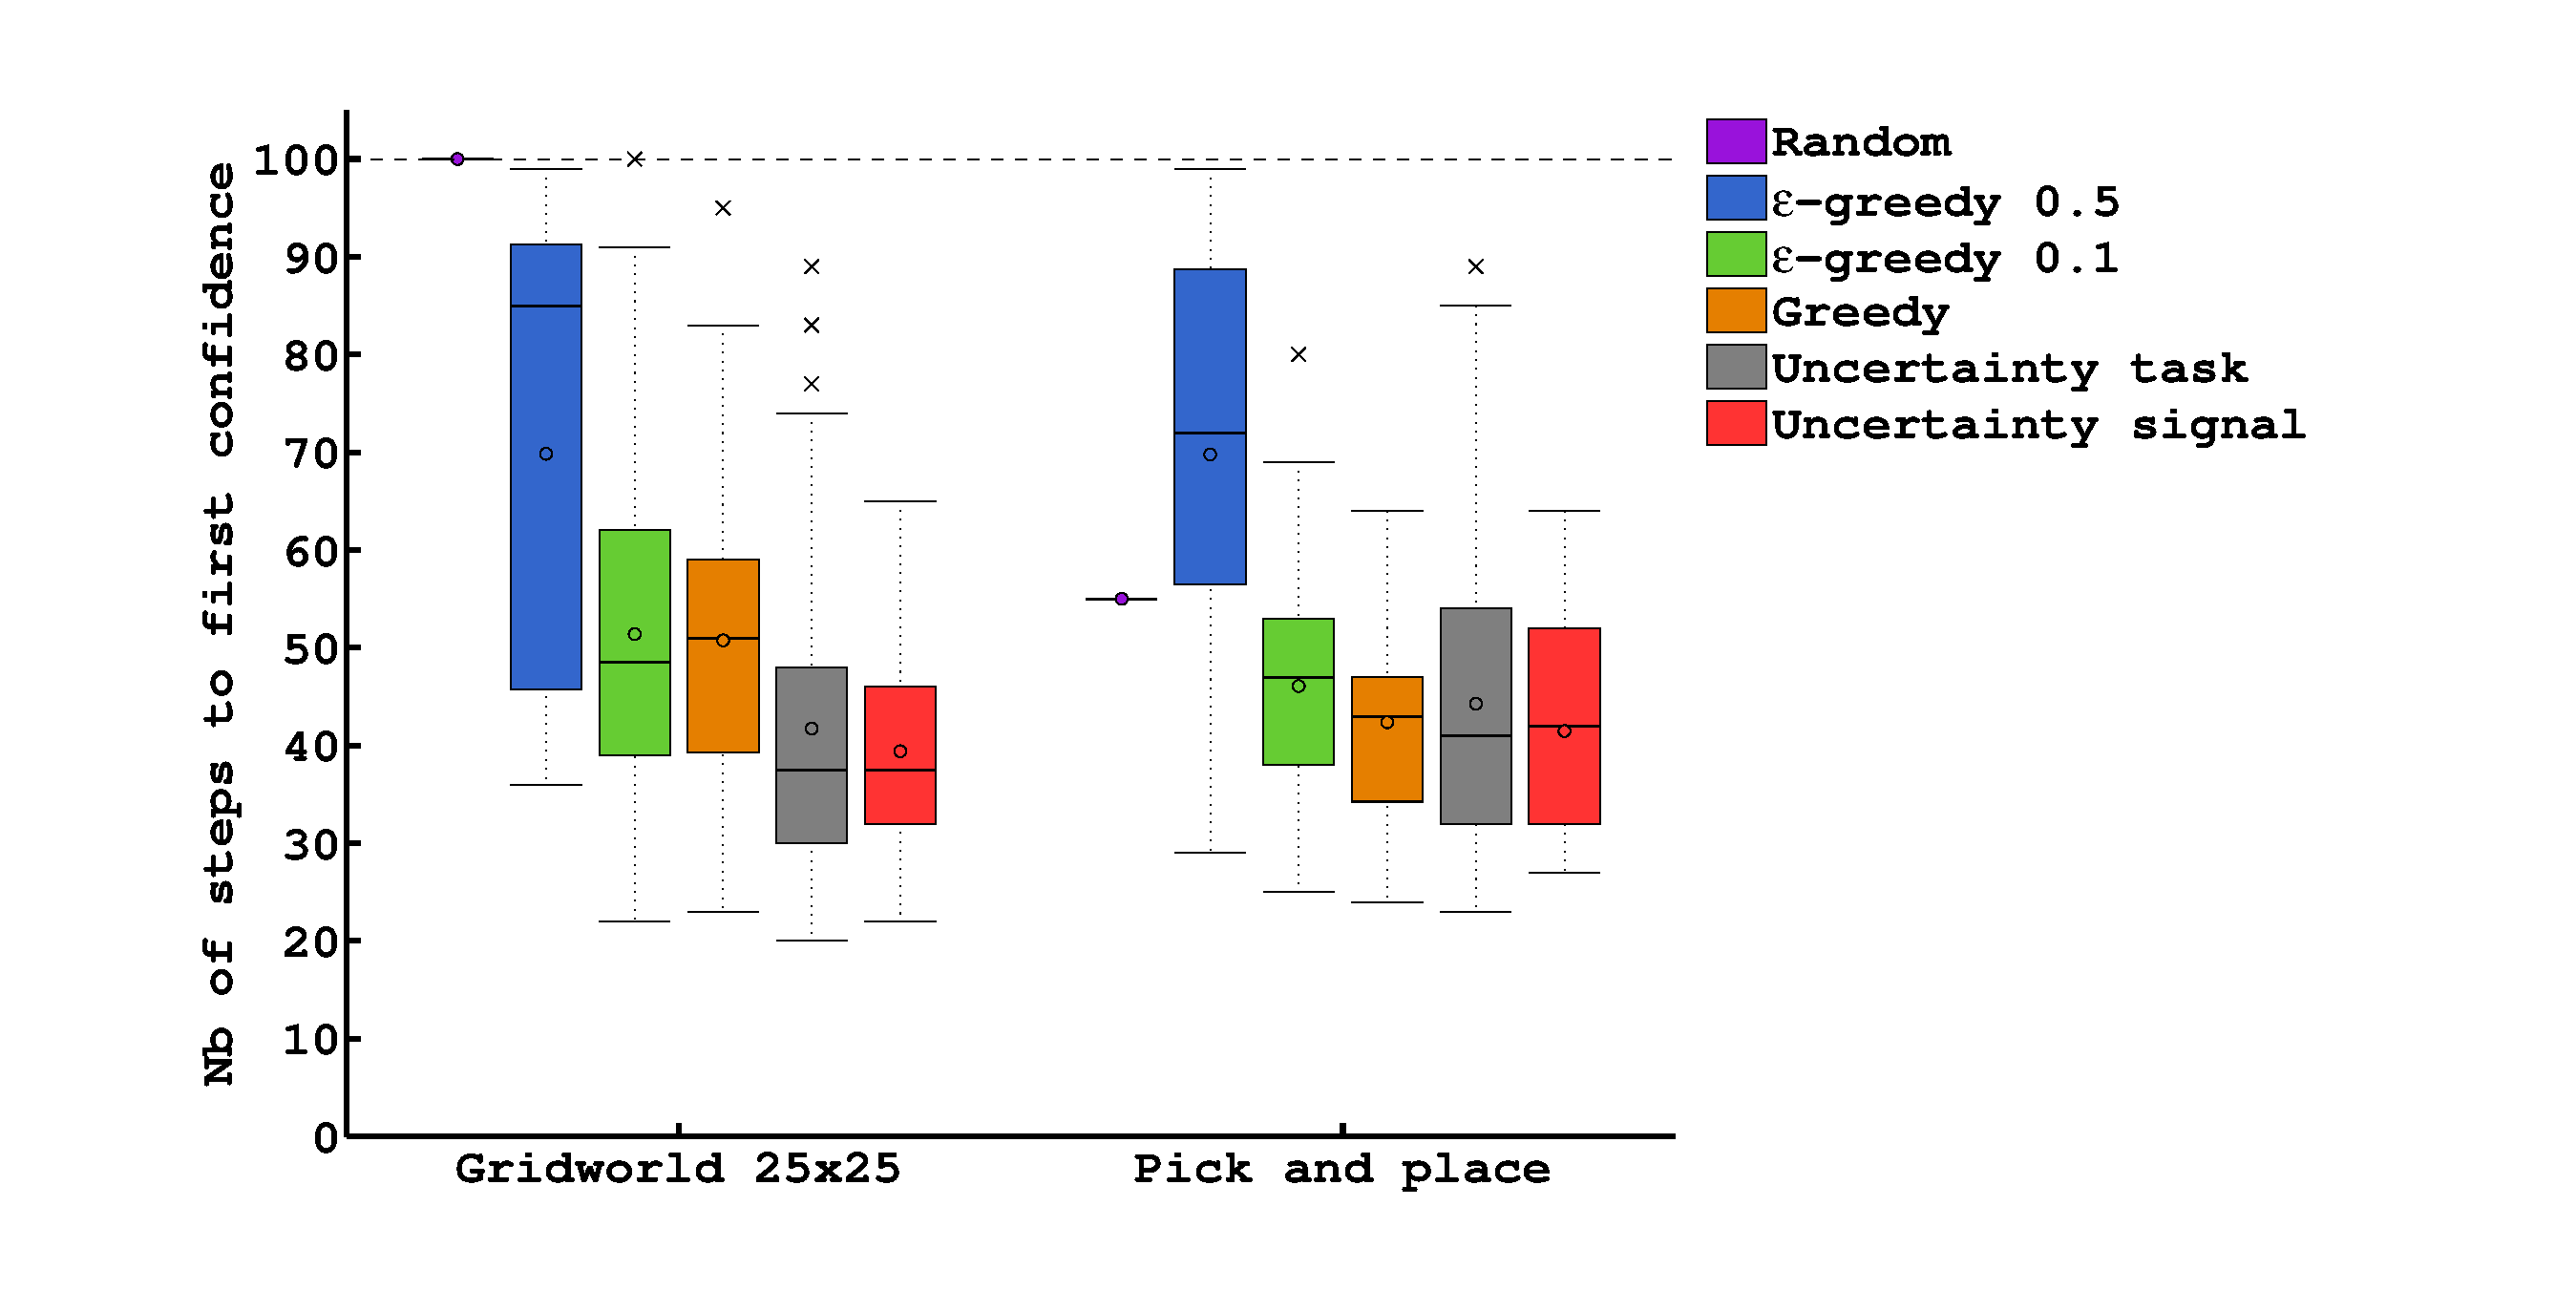
\includegraphics[width=\legendsidesize\columnwidth]{\imgpath/world_properties/firstconfident.eps}
\caption{Number of steps to reach confidence level for the first target.}
\label{fig:wordlpropertiesconfidencefirst}
\end{figure} 

Figure~\ref{fig:wordlpropertiestargetdist} shows the number of actions needed for the agent to reach the goal state once the task is identified with confidence. This plot only considers the runs where a target was reached (see Table~\ref{tab:wordlpropertiesnreach}). For the grid world, all planning methods identify the task less than 5 steps away from its associated goal state. However for the pick and place problem, by following our uncertainty based planning method the agent is on average 10 steps away from the goal state when it identifies a task with confidence.

\begin{figure}[!htbp]
\centering
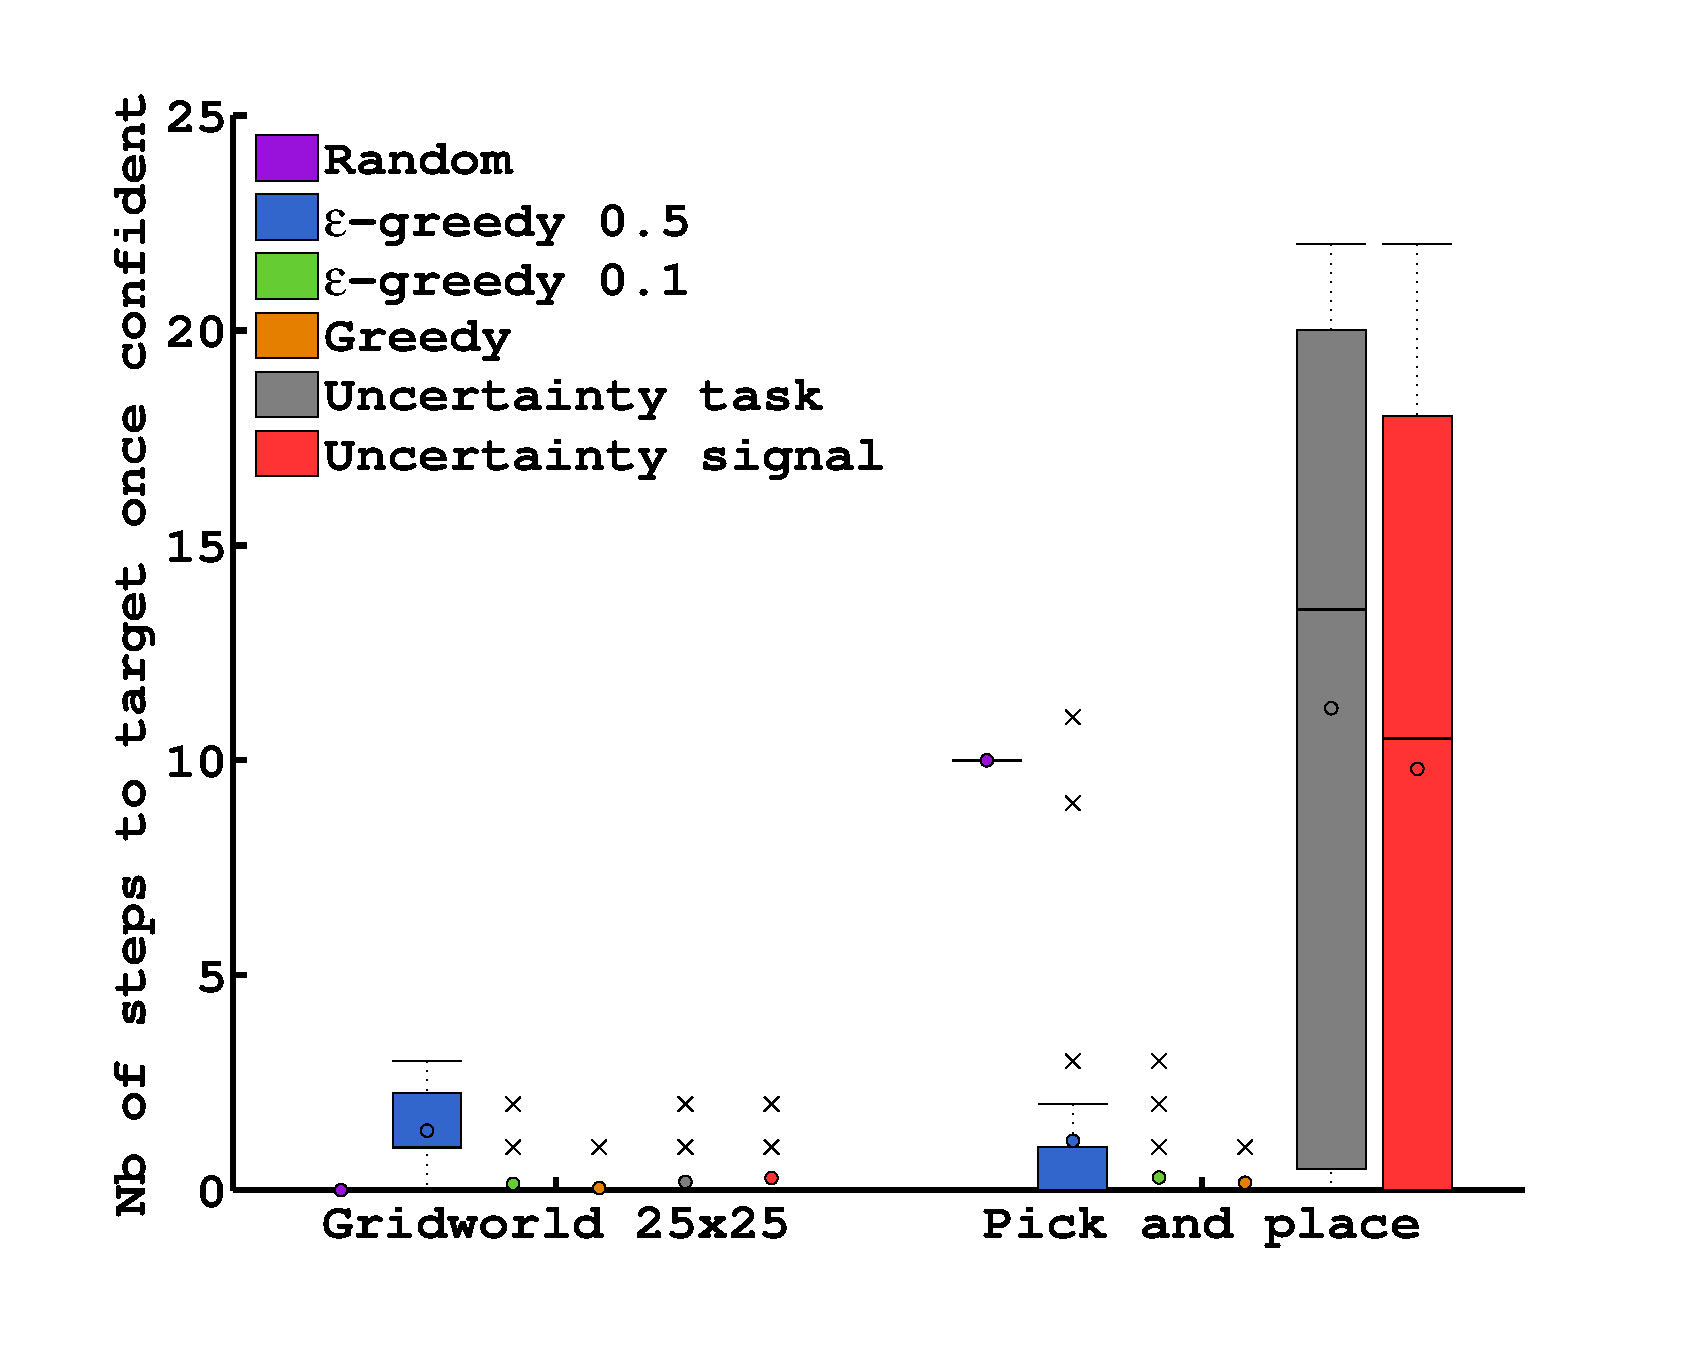
\includegraphics[width=\plotsize\columnwidth]{\imgpath/world_properties/difftargetconfidence.eps}
\caption{Number of actions needed to reach the first target once the agent reached confidence level for this target. This plot only consider the runs where a target was reached in less than 100 steps (see Table~\ref{tab:wordlpropertiesnreach}). Random action selection for the 25x25 grid world is not represented as it never reached any, and random for the pick and place only considers one run.}
\label{fig:wordlpropertiestargetdist}
\end{figure} 

We hypothesized that, given the maze like properties of the pick and place problem, our agent would need to go toward the best hypothesized target states to differentiate between them faster. And therefore that our uncertainty planning method may be more efficient in such case. This hypothesis is not confirmed and requires more investigation on what properties are actually influencing the efficiency of our algorithm and what additional metrics should be considered to improve our strategies. Indeed none of the method presented are considering their performance on the task (yet unknown but estimated) in the action selection process. 

% This is part of the discussion of next subsection.

\todo{We note that the greedy method is going towards the best hypothesis goal state, which confirms our intuition of what is a good planning strategy in such world, but does not explain why our uncertainty method ends-up far from the goal state when the confidence level is reached.}
% In order to explain this differences one should analyze the behavior of the agent and the evolution of the probability associated to each task, and check which group of tasks are ruled out first between the Greedy and the uncertainty based method that may explain the differences of behavior observed.

% Finally, as for the analysis of the size of the worlds, we note that in chapter~\ref{chapter:planning}~and~\ref{chapter:bci} the greedy method shows very poor performances for 30 dimensional signals. Therefore it is required to compare the performances of the planning methods for a variety of datasets with different dimensionality and quality.

\subsection{Discussion}

The main conclusion of this study is that we do not understand well the impact of worlds and datasets properties on the final performance of the system. Many of these properties are tightly linked together and the additional layer of uncertainty inherent to our problem makes the dependencies hard to identify.

However one important aspect highlighted by the study is that our uncertainty measure should be combined with other metrics to optimize additional criteria on the task. Our measure was developed to discriminate faster the correct hypothesis from the set of possible tasks and not to also execute that task as fast as possible.

On this basis, we propose two different types of scenario to investigate: 
\begin{itemize}
\item \textbf{Target based scenarios:} In these scenarios, the goal of the agent is to execute one specific action in a particular state, but in situation where failing the task have bad consequences. 
% In addition, it is important to succeed in the task. and should not make mistakes in the execution of the task. 
Lets consider a robot that should identify one object among a finite set and put it to the bin for a human. The robot can navigate freely around the objects in order to collect feedbacks from the human. However, the robot should only grasp and throw an object once it is confident that it is the object intended by the human. 
% This includes all the scenario considered in this thesis, and as seen in this section there is room to improve over our uncertainty method by including information about the hypothesized task.
This problem is an instantiation of the visual navigation task used in our BCI experiments. In chapter~\ref{chapter:limitations:wordlproperties}, we have seen that our uncertainty method can be outperformed by a simpler method (greedy) when the goal is to identify and perform the task as fast as possible. It is likely that a pure greedy method can be outperformed. The problem with our uncertainty measure was that the robot could disambiguate between task ``far away'' from their respective goal states. Requiring additional steps to reach the correct goal state once identified. A potential avenue is to merge our measure of uncertainty with information about the optimal policy of each task, such that, for two states of equal uncertainty, the state closer to the potential targets is preferred. The resulting problem lies in weighting between seeking for uncertainty reduction and optimizing the position of the agent with respect to the, yet unknown, goal state.

% When all task are equally probable, only the uncertainty should be taken into account. And once there is no more uncertainty, i.e. when confidence is reached, the action should be selected according to the task policy.

\item \textbf{Reward maximization scenarios:} In these scenarios, the goal of the robot is to maximize the cumulative reward associated to the correct task. The problem is that many tasks may have similar reward functions. Therefore it is not always necessary to identify the correct task with confidence to collect maximal rewards. For example, in our puddle word scenario of section~\ref{chapter:limitations:continousstate}, two tasks may share the same goal area but have different areas to avoid. If the robot can reach the shared goal area by avoiding the negative areas of both hypothesis, then the agent will have maximized the collected reward without ever knowing what specific task the user had in mind. In such case, the agent must known whether merging two reward functions is more optimal than trying to differentiate between them.
\end{itemize}
% %!TEX root = ../../thesis.tex

\section{Exploiting overlap between distributions}
\label{chapter:limitations:overlap}


In this section, we propose a method that uses the overlap between the model for each class to identify the correct task hypothesis, and demonstrate the efficiency of our uncertainty measure on the signal space presented in chapter~\ref{chapter:planning:uncertaintysignalspace}. We present simulated experiments using pre-recorded EEG signals, and show that we achieve similar performances than calibration based systems. Finally, we report online experiments where four users control, by means of a BCI, an agent on a virtual world to reach a target without any previous calibration process.

\subsection{Using the Bhattacharyya coefficient}

Following \cite{blankertz2010single}, we model the EEG signals using independent multivariate normal distributions for each class ($\mathcal{N}(\mu_c, \Sigma_c)$ and $\mathcal{N}(\mu_w, \Sigma_w)$). We will denote by $\theta$ this set of parameters $\{\mu_c, \Sigma_c,\mu_w, \Sigma_w\}$.

We propose to exploit the fact that when labels are mixed, the Gaussian corresponding to each classes should overlap more than for the correct label association (see Figure~\ref{fig:TworldLabelGaussian}). The Bhattacharyya coefficient measures this overlap, it has been related to the classification error of Gaussian models \cite{Kailath67} and is inversely proportional to the classification rate. Although there is no analytical relation between the coefficient and the classification rate, it is possible to derive bounds and good empirical approximations \cite{lee2000bayes}.

The Bhattacharyya coefficient $\rho \in [0,1]$ between the Gaussian distributions associated to label ``correct'' ($\mathcal{N}(\mu_c, \Sigma_c)$) and ``incorrect'' ($\mathcal{N}(\mu_w, \Sigma_w)$) is:

\begin{eqnarray}
\rho = e^{-D_B(\theta)}
\end{eqnarray}

where $D_B$ is the Bhattacharyya distance:

\begin{eqnarray}
D_B(\theta) = \frac{1}{8}(\mu_c-\mu_w)^T(\frac{\Sigma_c+\Sigma_w}{2})^{-1}(\mu_c-\mu_w)+\frac{1}{2}ln\left(\frac{det(\frac{\Sigma_c+\Sigma_w}{2})}{\sqrt{det\Sigma_c det\Sigma_w}}\right)
\end{eqnarray}

Finally, we approximate the expected classification rate as:
\begin{eqnarray}
Ecr \propto 1 - \rho
\end{eqnarray}

Now that we have an estimation of the expected classification rate, which is proportional to the overlap between the model of each class, we need to take a decision with respect to which task is the one intended by the user. To do so we compare the expected classification rate of every task hypothesis $\xi_t$ with $t \in \{1, \ldots, T\}$. 

The hypothesis whose associated model overlaps the less, i.e. which has the highest expected classification rate, i.e.\ the lowest value of $\rho$, is expected to be the one intended by the user. However it is meaningless to define an absolute threshold on the value of the expected classification rate itself. Indeed, different people generate different signals which result in classifiers of different qualities. Also, even the for the correct signal-label pairs, the model may overlap by quite some amount, as shown in our 2 dimensional examples in Figure~\ref{fig:datasetsquality}. To bypass this problem we rely on a voting system where we attribute to each hypothesis $\xi_t$ a weight that is updated at every iteration.

We rely on a pseudo-likelihood metric that for each hypothesis $\xi_t$ accumulates the expected classification rate over time:

\begin{eqnarray}
\L(\xi_t) = \prod_{i = 1}^{M} 1 - \rho_i^{\xi_t}
\end{eqnarray}
%
with $M$ the current number of iteration and $\rho_i^{\xi_t}$ the Bhattacharyya coefficient associated to task $\xi_t$ using all data up to time $i$. By normalizing the pseudo-likelihood values between every hypothesis, we obtain what can be viewed as the probability of each target:

\begin{eqnarray}
p(\xi_t) = \frac{\L(\xi_t)}{\sum_{u \in \{1, \ldots, T\}} \L(\xi_u)}
\end{eqnarray}

Once a target reaches a probability threshold $\beta$ we consider it as being the correct one, i.e.\ the one intended by the user. We used $\beta = 0.99$.

Finally, once we identified the first target, we will switch back to a classification based algorithm as described in chapter~\ref{chapter:lfui:tasttotask} and as used in the previous chapters of this thesis. We will see in section~\ref{chapter:limitations:overlap:offline} that this switch is necessary to maintain good performances since the classifier makes a much harder decision for each new EEG signal.

\subsection{Planning}

As we are using a model based method, we rely on our method measure that measure uncertainty directly in the signal space. This method was described in chapter~\ref{chapter:planning:uncertaintysignalspace} and to summarize rely on computing, for every state-action pairs, the similarity between the expected signals for each task. The more the expected signals are similar the less there is uncertainty.

For computing the similarity between two Gaussian distributions we could rely again on the Bhattacharyya coefficient describe above. However computing this coefficient between all models and for all state-action pairs was not feasible in real time. In order to improve computation efficiency we do not rely on a precise metric between Gaussian distributions and only consider the similarity between their means. The closest the means are, the more similar they are.

\subsection{Offline analysis}
\label{chapter:limitations:overlap:offline}

The objective of the offline analysis is to study the impact of our exploration method and evaluate if the classifier learned from scratch with our algorithm can be reused for learning new tasks. To ensure we have sufficient data to achieve statistically significant results, we rely on a large dataset of real EEG data. We used the same dataset as describe in chapter~\ref{chapter:bci:EEGsignals} dataset from \cite{iturrate2013task}, which covers ten subjects that performed two different control problems.

For each subject, we simulated 20 runs of 400 iterations following the control task. Each time the device performed an action, we sampled the dataset using the ground truth labels corresponding to the correct task and then removed the chosen signal from it. After a first task was identified we continued running the system to identify new tasks. 

We present most of the results in terms of the quality of the dataset, measured as the classification accuracy that a calibrated brain signal classifier would obtain.

\paragraph{Planning Methods}

We compared the average number of steps (with maximum values of 400 steps) needed to identify the first task when learning from scratch with different planning methods.

\begin{figure}[!ht]
    \centering
    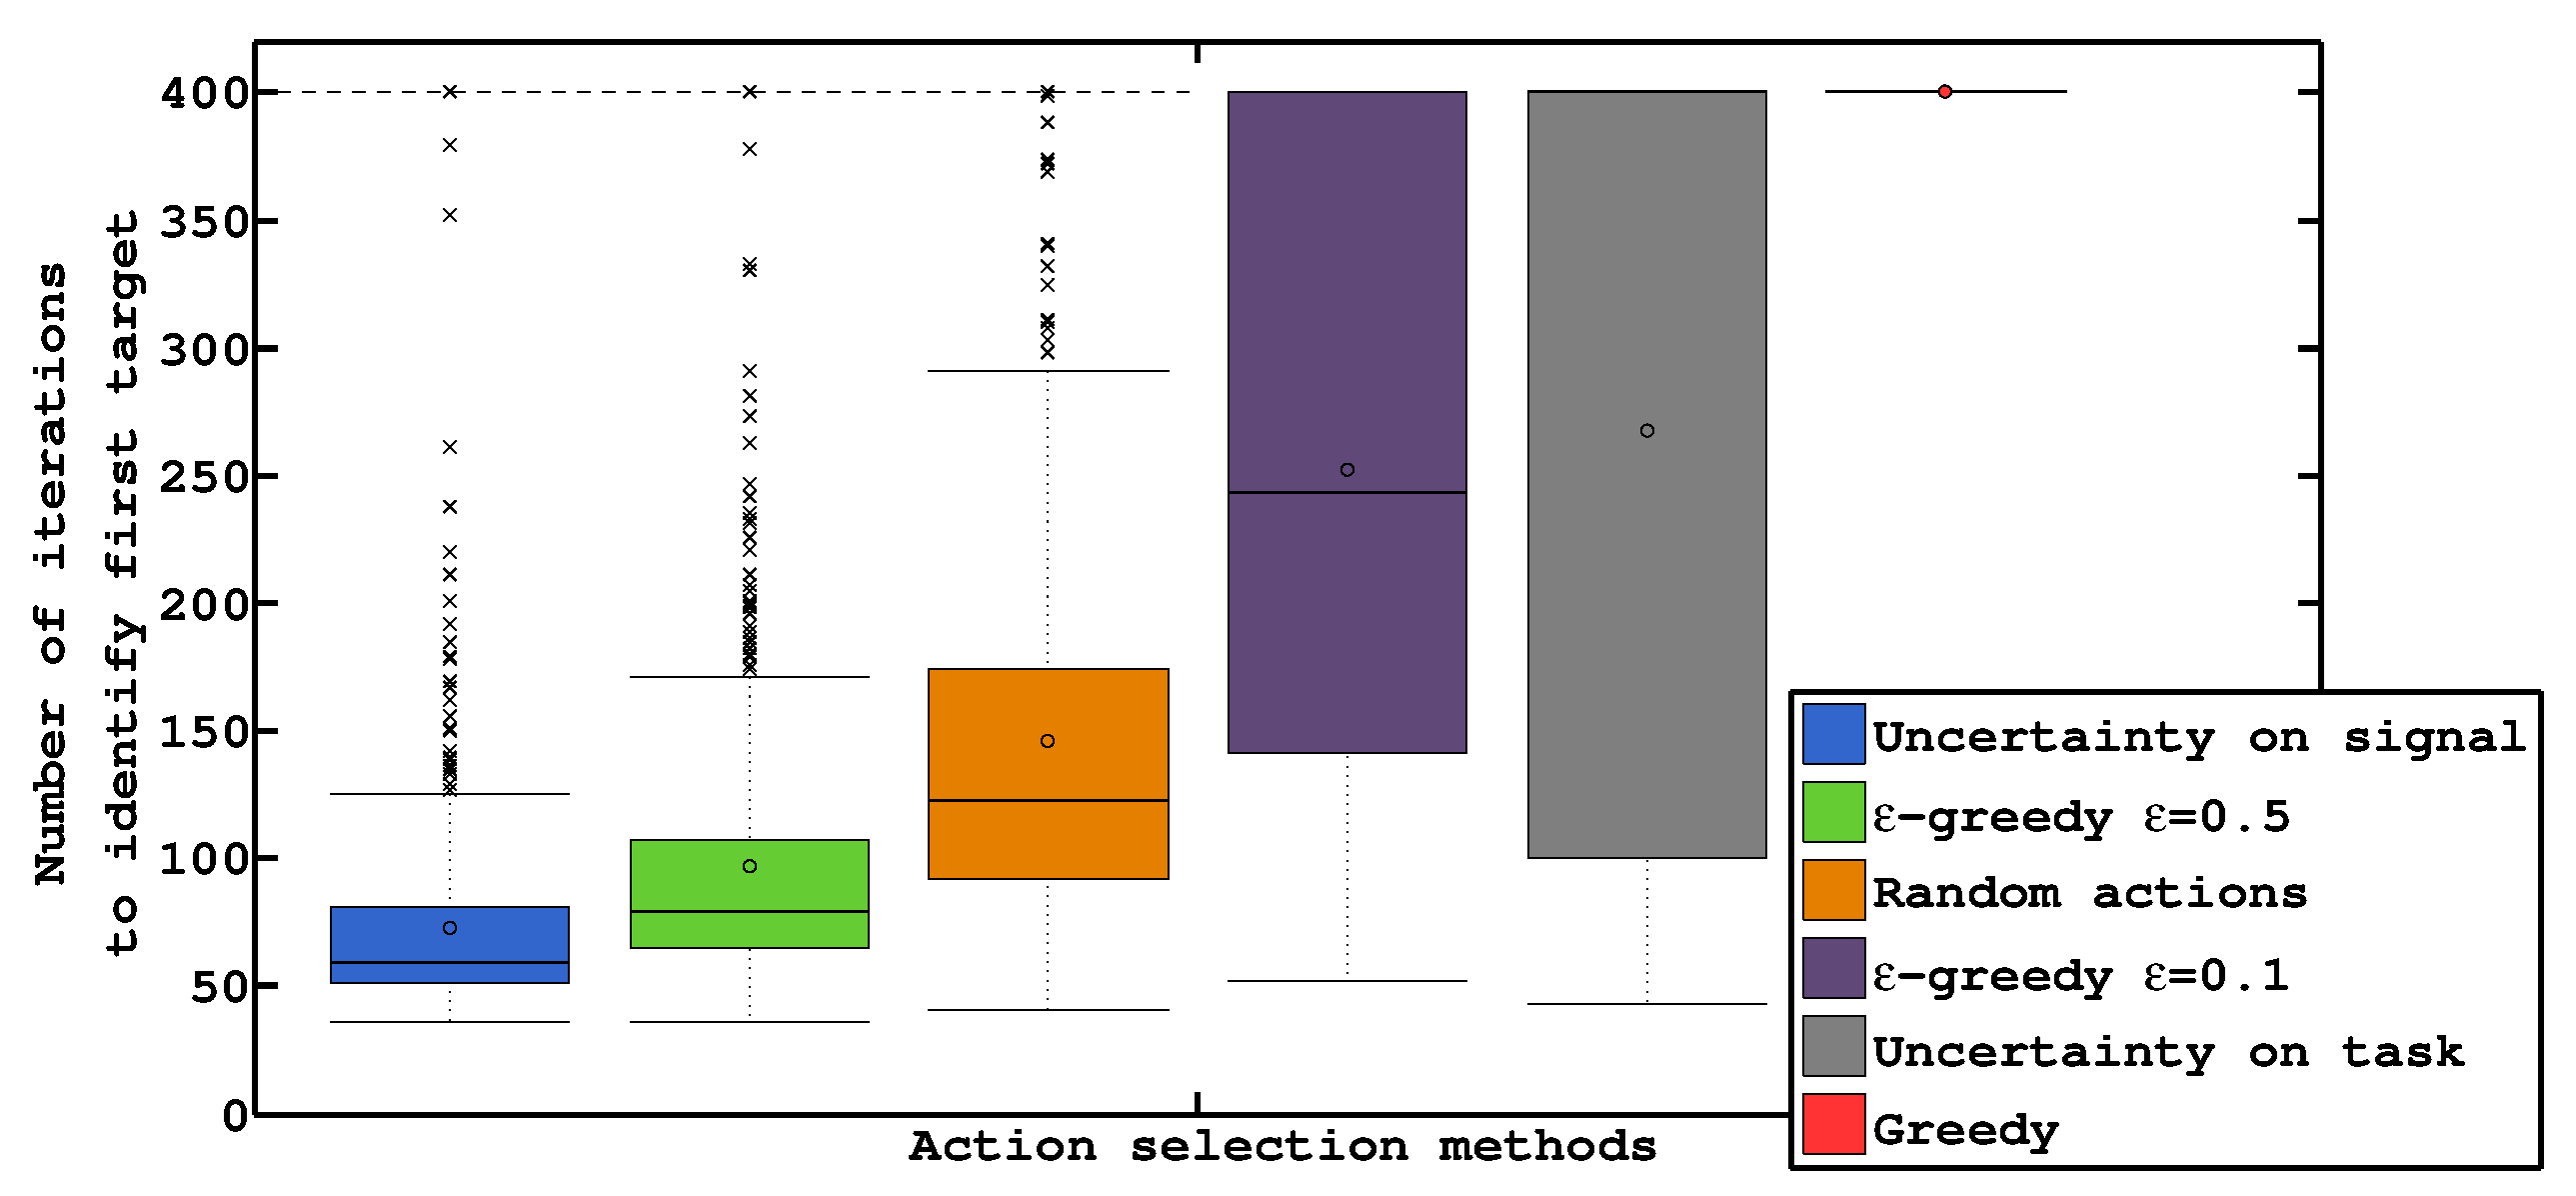
\includegraphics[width=\columnwidth]{\imgpath/battacharyya/plot_planning_first.eps}
    \caption{Comparison of different exploration methods. Our proposed method, based on the uncertainty on the expected signal, allows to lead the system to regions that improve disambiguation among hypotheses in a faster way. For the greedy method, all values were 400 which indicates it never allowed to identify any task.}
    \label{fig:overlapcompplan}
\end{figure}

Figure~\ref{fig:overlapcompplan} shows the results averaged across subjects, runs and datasets. Values of 400 means the confidence threshold was not reached after 400 iterations. Our proposed method, based on the uncertainty on the expected signal, allows to lead the system to regions that improve disambiguation among hypotheses in a faster way. Trying to follow the most probable task does not allow the system to explore sufficiently (Greedy), and at least some random exploration is necessary to allow a correct identification of the task ($\epsilon$-greedy). Assessing uncertainty only on the task performs poorly as it does not take into account the signal interpretation ambiguity inherent to our problem. The large variability in the results is mainly due to the large variations in classification accuracy across subjects and datasets. Given these results, the remainder of this section will only consider our proposed planning method.

\paragraph{Using the Bhattacharyya coefficient in the long run}

After identifying the first task, and following our approach, we continued running the system and measured how many tasks were identified after 400 steps. Figure~\ref{fig:overlapbhatta} demonstrates the advantage of switching to a classification based method after identification of a first target instead of keeping the estimation given by the Bhattacharyya coefficient. On the one hand, Bhattacharyya coefficient works very well for small amounts of data because it directly compares model parameters. On the other hand, after identifying many task, all models share most of their signal-label pairs and it requires much more data to modify the models and detect overlaps. Therefore using a classifier allows for a faster identification since the classifier makes a much harder decision for each new EEG signal. This discussion is in line with the observation on the use of the power information made in chapter~\ref{chapter:bci:priorpower}.

\begin{figure}[!ht]
    \centering
        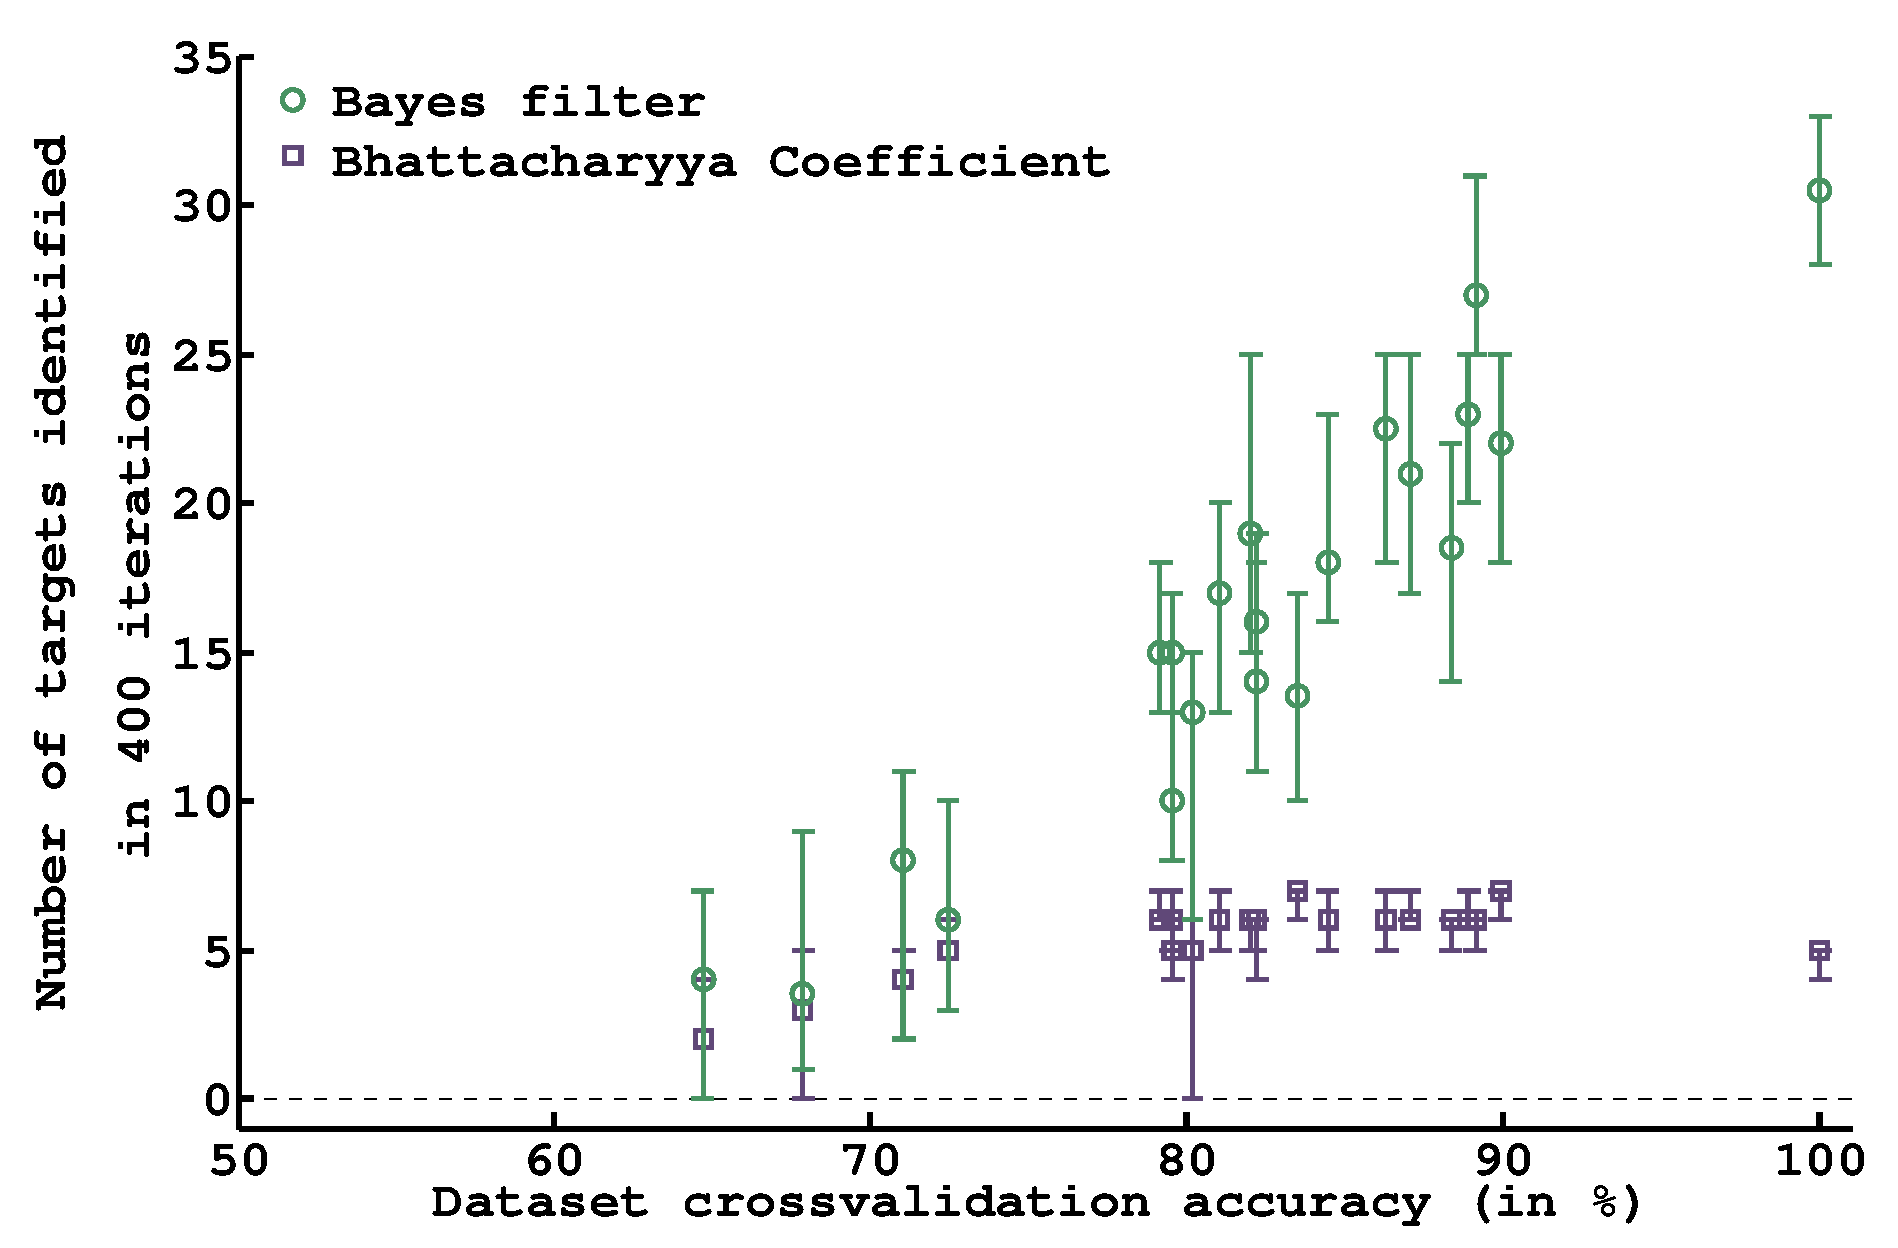
\includegraphics[width=\plotsize\columnwidth]{\imgpath/battacharyya/plot_bhattha_vs_bayes}
        \caption{Number of targets correctly identified in 400 iterations (the markers show the median values and the error bars the 2.5th and 97.5th percentiles). Comparison between switching to a Bayes filter method after identification of a first target instead of keeping the estimation given by the Bhattacharyya coefficient. The classification based method allows for a faster identification.}
        \label{fig:overlapbhatta}
\end{figure} 

Given these results, in the remaining of this section we only consider switching to a classification based method once the first task has been identified.

\paragraph{After 400 steps}

Figure~\ref{fig:overlapavg_sum_400} shows the number of tasks correctly and incorrectly identified in 400 iterations. For datasets of good qualities, we are able to identify more than 20 tasks in 400 iterations without the need for a calibration procedure (recap that previous works needed between 300 and 600 examples for the calibration phase \cite{chavarriaga2010learning,iturrate2010single}). The number of correctly identified tasks is strongly correlated to the quality of the dataset.

\begin{figure}[!ht]
    \centering
    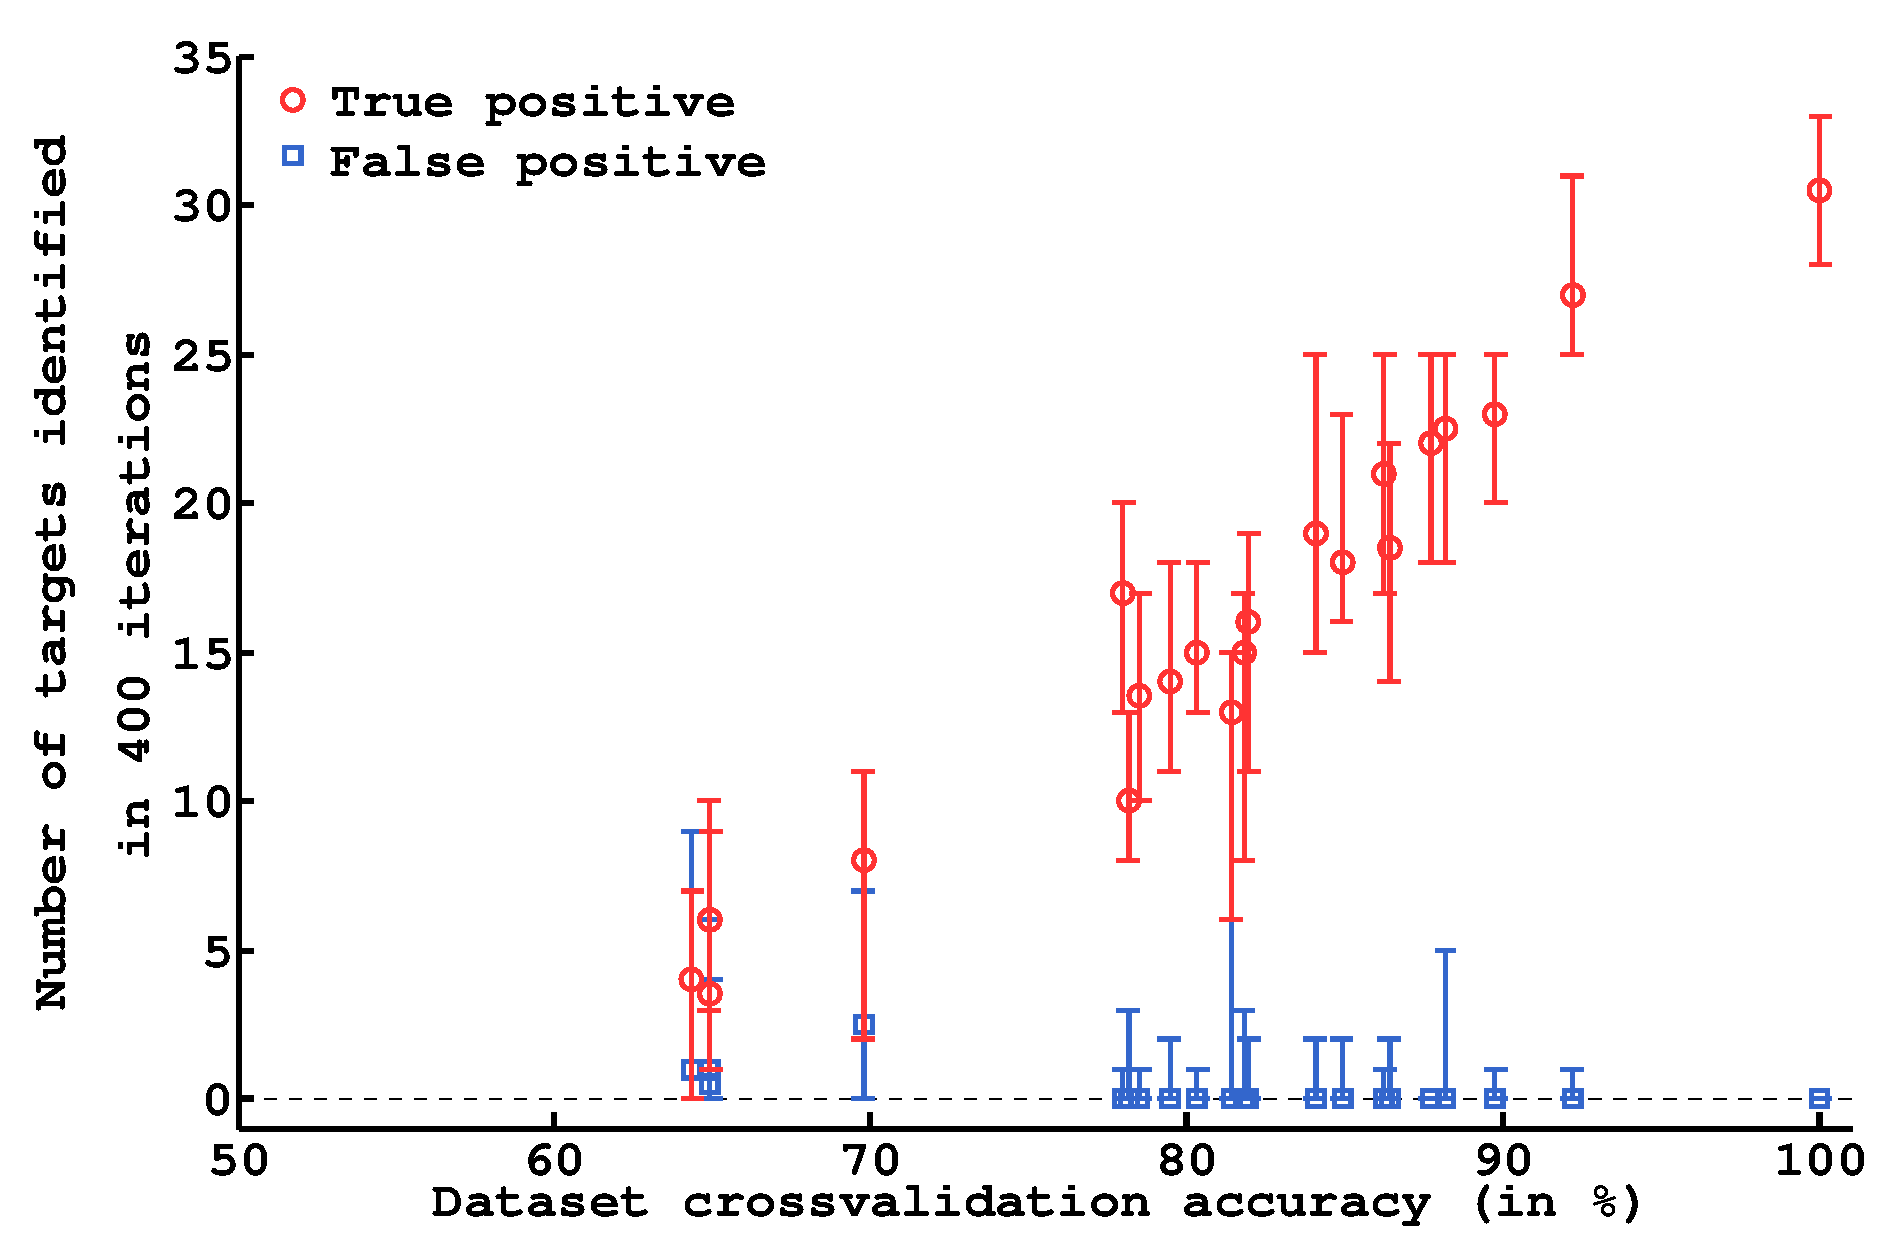
\includegraphics[width=\plotsize\columnwidth]{\imgpath/battacharyya/plot_first400_reach} 
    \caption{Number of targets correctly and incorrectly identified in 400 iterations (the markers show the median values and the error bars the 2.5th and 97.5th percentiles). For datasets of good qualities, we are able to identify more than 20 tasks in 400 iterations without the need for a calibration procedure.}
    \label{fig:overlapavg_sum_400}
\end{figure} 

The quality of our unsupervised method can be measured according to the percentage of labels correctly assigned (according to the ground truth label), see Figure~\ref{fig:overlappercentageLabels}. In general, having dataset with classification accuracies higher than 75$\%$ guaranteed that more than 90$\%$ of the labels were correctly assigned. This result shows that our algorithm can also be used to collect training data for calibrating any other state-of-the-art error-related potentials classifier, but has the important advantage of controlling the device at the same time.

\begin{figure}[!ht]
    \centering
        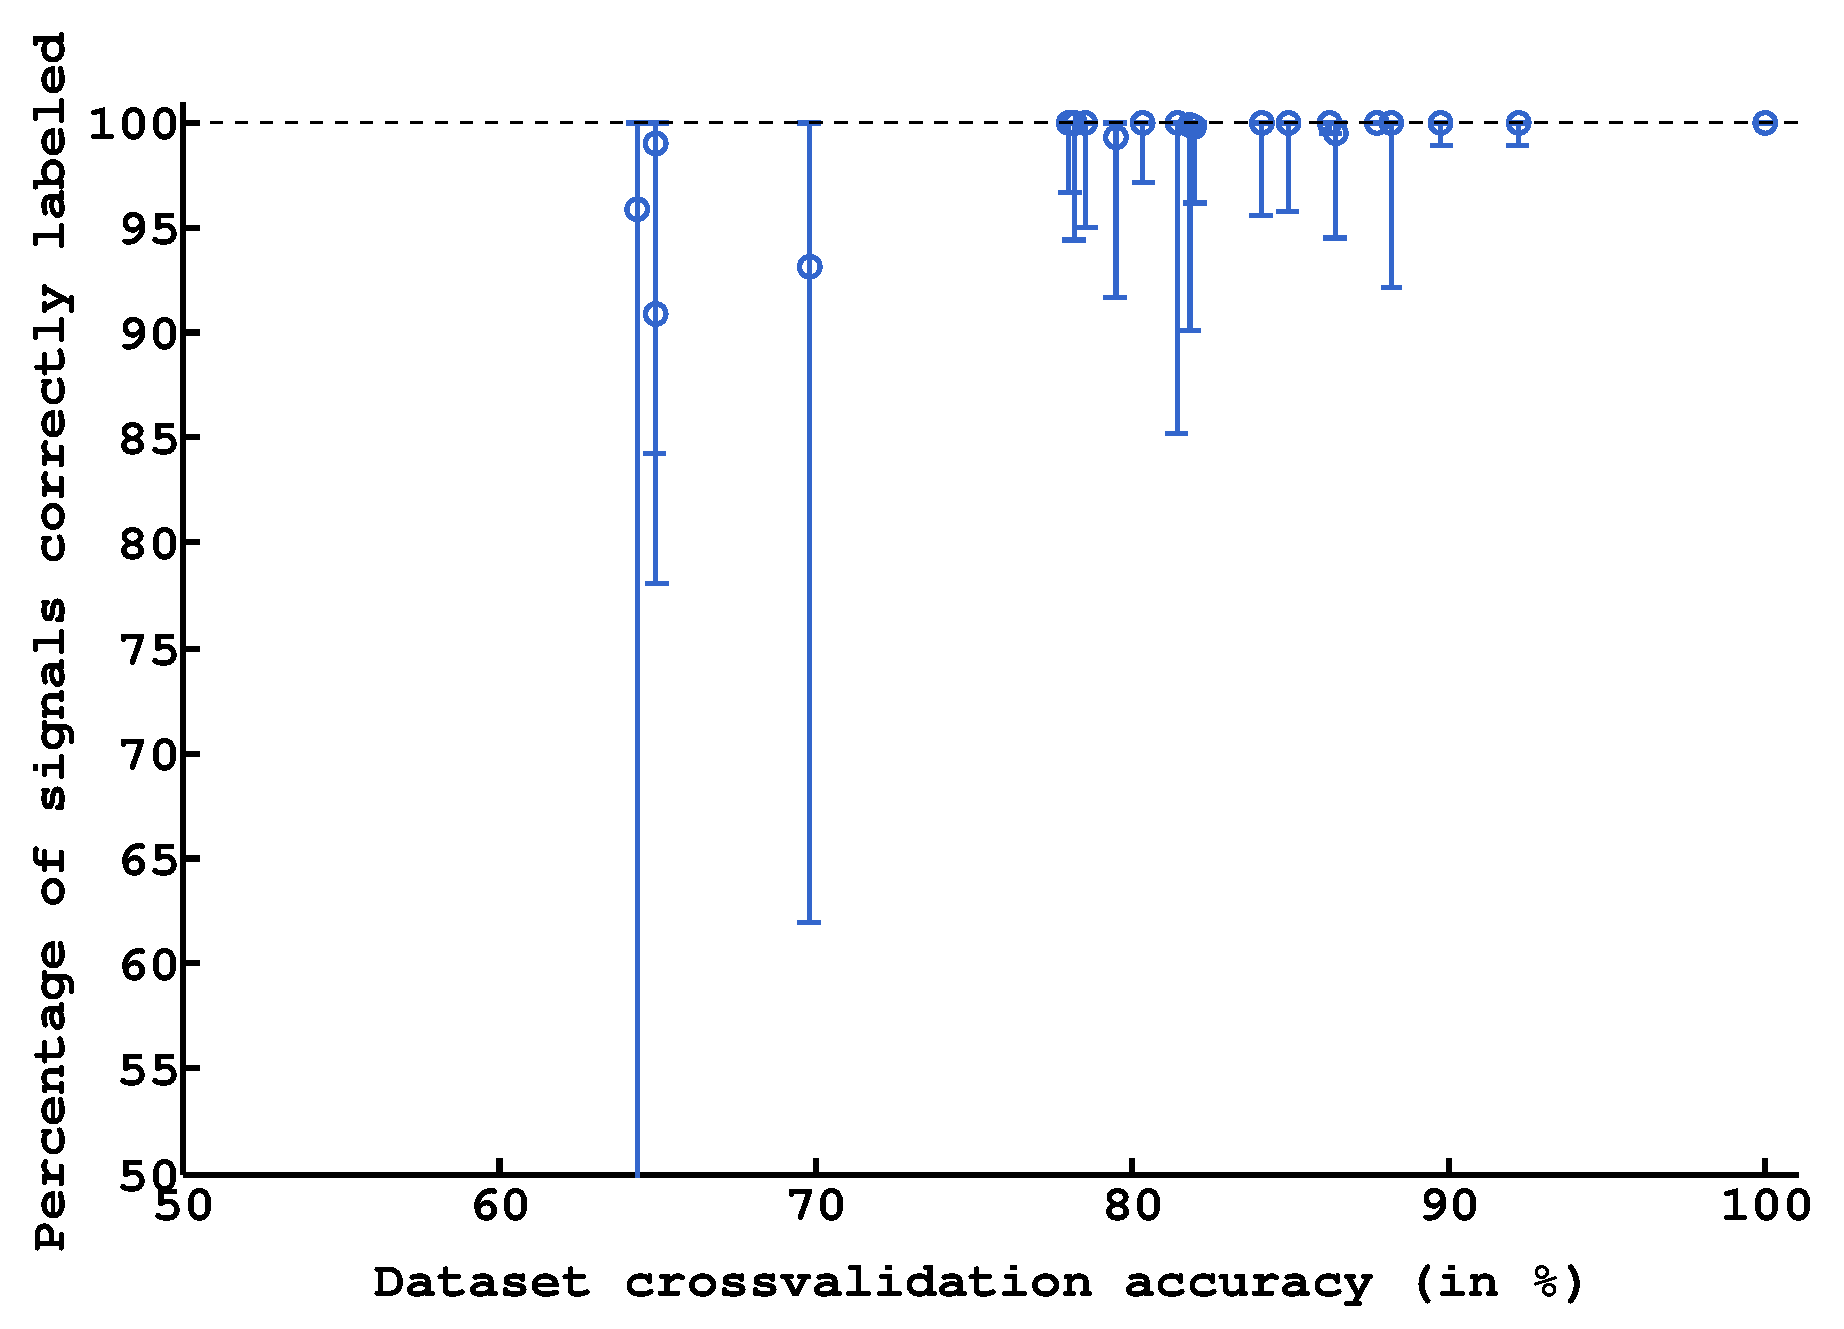
\includegraphics[width=\plotsize\columnwidth]{\imgpath/battacharyya/plot_percent_label}
        \caption{Percentage of labels correctly assigned according to the ground truth label (the markers show the median values and the error bars the 2.5th and 97.5th percentiles). In general, having dataset with classification accuracies higher than 75$\%$ guaranteed that more than 90$\%$ of the labels were correctly assigned.}
        \label{fig:overlappercentageLabels}
\end{figure}

\subsection{Online control}

The experiments were conducted with four subjects (aged between 25 and 28). Each subject was asked to mentally assess the agent's actions with respect to a given target. The system was not calibrated to decode the user EEG signals beforehand. Each subject performed 5 runs, for each run a new target was randomly selected and provided to the user. There was an action every three seconds. Each run lasted 200 actions, and the time between runs was around one minute.

The algorithm was able to identify the correct target for all runs of all the subjects, see Figure~\ref{fig:overlaponlineresults}. There are strong variations among subjects but we note that our system identified each task in less iterations than a normal calibration phase requires (between 300 and 600 examples depending on the user performance \cite{chavarriaga2010learning,iturrate2010single}).

\begin{figure}[!ht]
    \centering
    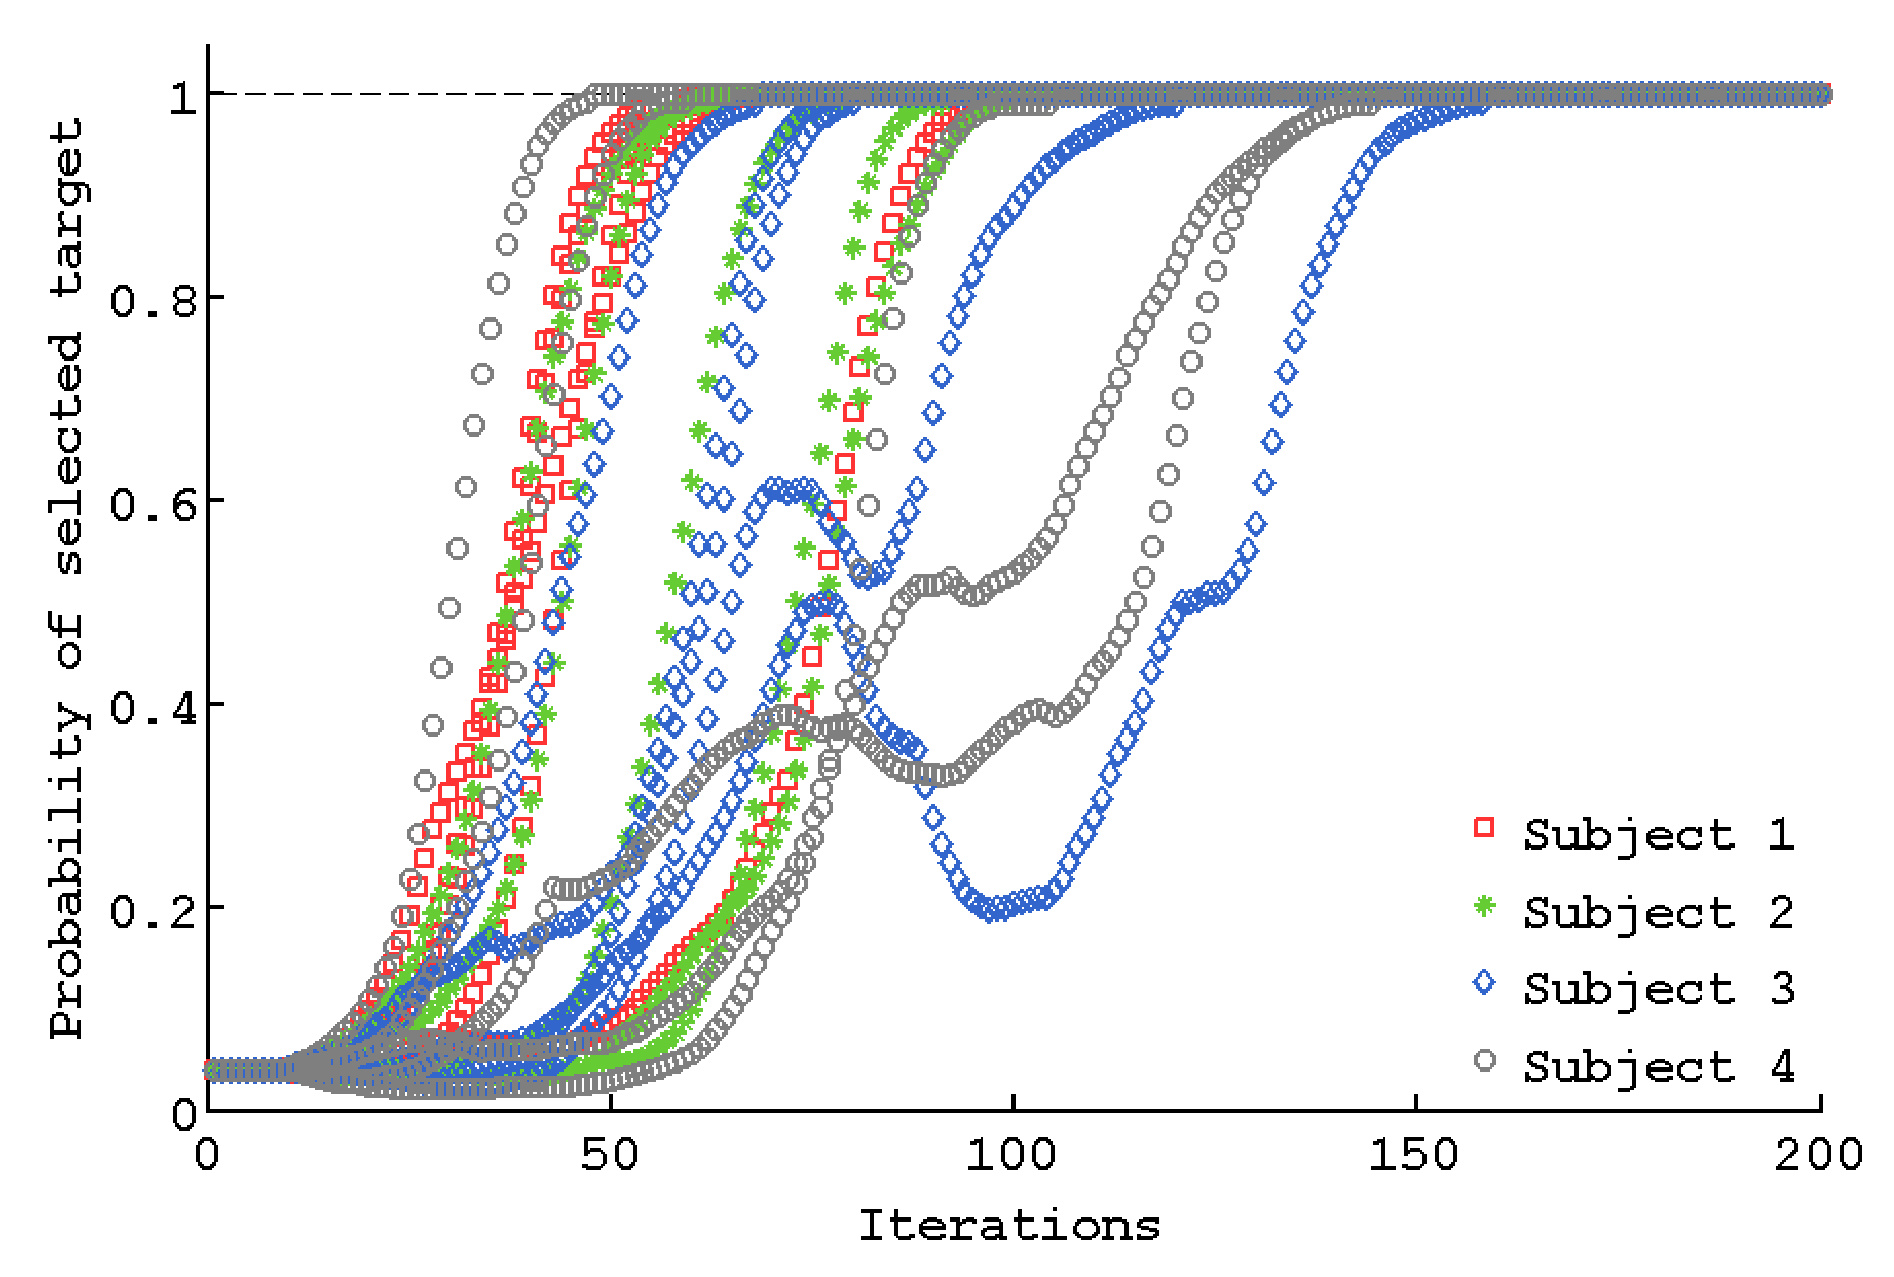
\includegraphics[width=\plotsize\columnwidth]{\imgpath/battacharyya/plot_realevolution}    
    \caption{Results from the online experiments: Evolution of the probability of the correct task for each subject and run. The algorithm was able to identify the correct target for each subjects and runs in less than 200 iterations.}
    \label{fig:overlaponlineresults} 
\end{figure}

Table~\ref{tab:overlaponline} shows for each subject and run the number of iterations needed to reach the confidence threshold for the subject selected target.

On average, the number of iterations needed to identify the target was of 85 $\pm$ 32.

\begin{table}[!ht]
\centering
\rowcolors{2}{gray!25}{white}
\begin{footnotesize}
\begin{tabular}{r|rrrrr|r}
    %\toprule
    & \textbf{Run1} & \textbf{Run2} & \textbf{Run3} & \textbf{Run4} & \textbf{Run5} & \textbf{mean$\pm$std} \\\hline
    %\midrule
    \textbf{S1} & 95 & 62 & 56 & 60 & 64 & 67 $\pm$ 16 \\
    \textbf{S2} & 89 & 77 & 98 & 60 & 62  & 77 $\pm$ 17 \\
    \textbf{S3} & 68 & 80 & 118 & 76 & 157 & 100 $\pm$ 37 \\
    \textbf{S4} & 98 & 142 & 57 & 142 & 47 & 97 $\pm$ 45 \\
\end{tabular}
\end{footnotesize}
  \caption{Results from the online experiments: Number of iterations needed to identify the correct target for each subject and run. On average, the number of iterations needed to identify the target was of 85 $\pm$ 32.}
  \label{tab:overlaponline}
\end{table}

\subsection{Discussion}

We introduced a new method to exploit the facts that, when associated hypothetic labels to all task hypothesis, only the correct task assign the correct labels to the correct hypothesis. This method compares directly the overlap between the distribution modeling the generation of such signals. As for wrong hypothesis, the labels tend to be mixed with respect to the underlying structure of the data, the overlap between distribution is a good and stable measure. 

However, we have seen that once all hypothesis share the same signal-label pairs, this method requires to collect more and more data to detect a change in the overlap of the wrong hypothesis. As a consequence the system should make use of two different sets of equations, one specific to the first target and one for the forthcoming targets.

This latter aspect shows the important advantage of the method we presented in this thesis, which only make use of one equation from the first to the last iteration. This equation captures both phase of the interaction, where during a first phase the classifier qualities are playing a major role, and in a second phase the classifier predictions are taking the lead by taking more hard decisions.
% %!TEX root = ../../thesis.tex

\section{A frame is a generic function}
\label{chapter:limitations:framegeneric}

\todo{A frame can be more complex than the simple relation described above. For example, a frame could include the gaze of the user as an indication of the user attention, therefore influencing the probability that the user is making a teaching mistake. For example, if the user is looking away from the scene, he is less likely to provide correct feedback. A frame is also not always related to the actions of the agent, it can be that, when the user show an object to the robot, he also spell the name of that object. This frame allows the robot to learn the name of different objects, this frame is often used in language acquisition experiments (see chapter~\ref{chapter:related:language})}


In this section, we provide example of what a frames might be. In all the experiment consider until now, we only considered the feedback and guidance frame which implies many constraint on the interaction protocol and the abilities of the robot. For example, the user should deliver feedback after one action of the robot, this simple interaction already requires to implement a turn taking social behavior in the robot, but also means that the user is able to see know when one action has been executed by the robot. On the other side, the robot need to interpret the signal from the user with respect to many objectives, and in our scenarios, this requires the robot to know the optimal plan in each state and for every task hypothesis. This kind of constraints are usual in BCI scenario, where it is still difficult to extract information continuously from ErrP EEG signals and where the task to be execute is often discrete and of low complexity such that it is easy for our agent to compute the optimal policies for each task. In the following of this section we describe a few frame that may be considered for extending this work to more real world robotic scenario.

\subsection{A task is not always a fixed target}

In this thesis, we only considered task which where represented as a sparse reward function represented in the MDP framework. However there is explicit reason of being limited to this choice, and especially the fact that one task represents a particular state of the world. A task may be an endless repetition of action such as for a robot in an assembly line that should be taught to assemble a given object again and again. Or a robot that should patrol around houses. 

For our feedback and guidance frame, as soon as the policies associated to each task can be provided to the robot, our algorithm scan be applied. We present in Figure~\ref{fig:gridwolrdgenericframes} two examples where policies are easy to define but are not always possible to derive in a simple MDP representation.

The policy of Figure~\ref{fig:gridwolrdgenericframesaround} consist of following the external wall of the grid world in a clockwise direction. This policy can not be derived from a state based reward function. Similarly in Figure~\ref{fig:gridwolrdgenericframesaround}, the policy consist of a endless looping trajectory, which can not be described by a reward function on our 9 states space. This kind of policies are rather easy to define by hand or by randomly generating them on a computer. 

\begin{figure}[!htbp]
\centering
    \begin{subfigure}[b]{0.49\columnwidth}
        \centering
        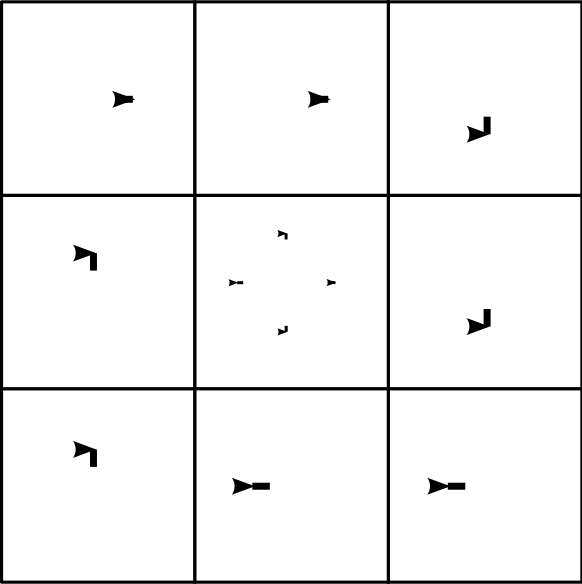
\includegraphics[width=0.8\columnwidth]{\visualspdf/frame/gridworld_around.pdf}
        \caption{W}
        \label{fig:gridwolrdgenericframesaround}
    \end{subfigure}
    \begin{subfigure}[b]{0.49\columnwidth}
        \centering
        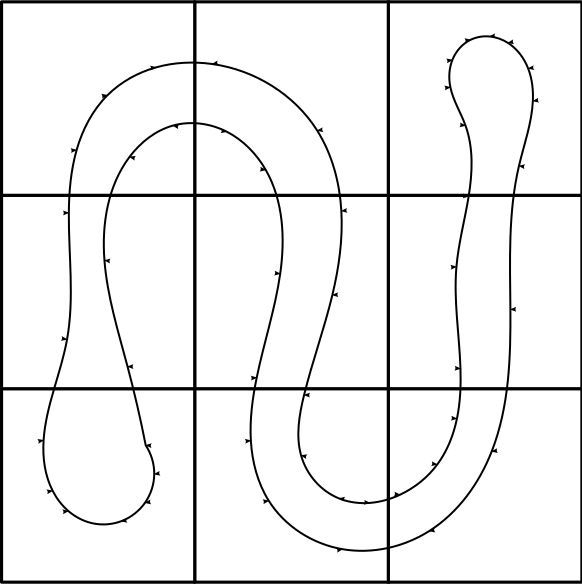
\includegraphics[width=0.8\columnwidth]{\visualspdf/frame/gridworld_loop.pdf}
        \caption{W}
        \label{fig:gridwolrdgenericframesloop}
    \end{subfigure}
\caption{Two examples of desired agent behavior that are harder to define in terms of rewards function.}
\label{fig:gridwolrdgenericframes}
\end{figure}

We note that it is always possible to represent the problems such that a fixed reward function allows to infer the policies of Figure~\ref{fig:gridwolrdgenericframesaround}~and~\ref{fig:gridwolrdgenericframesloop}. For Figure~\ref{fig:gridwolrdgenericframesaround} defining a reward function on the state-action space would be enough. For Figure~\ref{fig:gridwolrdgenericframesloop}, it is more challenging as the Markov properties are not respected, indeed it is necessary to known the previous position of the agent to predict its future position. Therefore the representation of the agent state should include the previous position of the agent, which increases the state space from 9 states to 81 states.

\subsection{No need for planning skills}

We provide an example of interaction frame where the agent do not need to know the optimal policy to interpret a signal with respect to a particular objective. In this frame, the goal of the robot is to locate one object or find one particular position in a 2D space. The teacher provide indication on the absolute direction of such object with respect to the agent position. As an example, we consider a teacher that indicates the cardinal direction of the object, i.e. the message to the robot is: \emph{``the object is North (South, West or East) with respect to your position''}.

We illustrate this frame in Figure~\ref{fig:cardinalframe}. The choice of the cardinal direction to send to the agent is modeled by a probabilistic models, where the probability of one cardinal direction is proportional to the angle between the target-agent direction and the cardinal direction considered.

\begin{figure}[!htbp]
    \centering
    \includegraphics[width=0.8\columnwidth]{\visualspdf/frame/cardinal_frame.pdf}
    \caption{Example of the cardinal frame. The signal from the teacher indicates in which cardinal direction (N,S,W,E) the goal position or the object to reach is. There is a probabilistic model that describe the user behavior, such that the probability of generating a signal of meaning ``West'' is proportional to the angle between the agent position and the target position. This frame does not requires the agent to know how to reach the target position, but only its own position with respect to that goal.}
    \label{fig:cardinalframe}
\end{figure}

We defined as $\varphi_N$ the angle between the target-agent direction and the North cardinal direction, and respectively $\varphi_S$, $\varphi_W$, and $\varphi_E$ the angles with respect to the South, West, and East directions. The probability of that the user refers to the North cardinal direction is defined as follows:

\begin{equation}
    p(l^f = \emph{north}~|~\varphi_N) = 
    \begin{cases}
    (1 - \frac{2 \varphi_N}{\pi}) (1-\alpha) & if~\varphi_N < \frac{\pi}{2}\\
        \frac{\alpha}{K}  & \text{otherwise}\\
   \end{cases}
   \label{eq:cardinalframe}
\end{equation}
with $K$ the number of cardinal direction that do not satisfies the condition $\varphi_N < \frac{\pi}{2}$, which means K can take value of 2 or 3 only. $\alpha$ is the error rate of the user. Finally, we consider unsigned angles only within the $[0, \pi]$ intervals only, meaning that angles of $\frac{-\pi}{2}$ or $\frac{3\pi}{2}$ are taken as $\frac{\pi}{2}$. The same equation applies for all cardinal direction and should maintain the following properties $\sum_{c \in \{N,S,E,W\}} p(l^f = c |\varphi_c) = 1$.

In practice, if we consider our visual representation of Figure~\ref{fig:cardinalframe}, we obtain the following angle measurements: $\varphi_N = \frac{9\pi}{22}$, $\varphi_S = \frac{13\pi}{22}$, $\varphi_W = \frac{20\pi}{22}$, and $\varphi_E = \frac{\pi}{11}$. In that case $K = 2$. If we consider $\alpha = 0$, we obtain the following probabilities values: $p(l^f = \emph{north}~|~\varphi_N) = 0.18$, $p(l^f = \emph{south}~|~\varphi_S) = 0$, $p(l^f = \emph{west}~|~\varphi_W) = 0$, and $p(l^f = \emph{east}~|~\varphi_E) = 0.82$, which we represent as a vector $[0.18,0,0,0.82]$. If we account of some probability of errors from the teacher, taking for example $\alpha = 0.05$, we obtain the following vector of probability: $[0.17, 0.025, 0.025,0.78]$.

We will use this frame in our experiment of section~\ref{chapter:limitations:continuoushypothesis}. Note that the same frame can apply with different referential, instead of the cardinal direction, one could refer to the direction with respect the robot orientation, or with respect to the position of the human teacher in the room, etc.

\subsection{Asynchronous instructions}

The interaction between our users and our robot would be easier if the robot could act continuously and the human would provide instruction when he deemed necessary. For example, in our pick and place scenario of chapter~\ref{chapter:lfui} it is boring for the user to provide feedback after each movement of the robot, it would be easier to wait the robot has displaced a cube to an other location. In addition, in some domains, the frequency of action is to high to afford waiting for a feedback signal between each action. Either the action would be so small that the user would not be able to judge the action, either the interaction flow would be dramatically affected by the many pauses in the task execution.

To allow for continuous operation of the robot, asynchronous delivery of signals should be accepted. A potential avenue is to consider a temporal function that distribute a signal event across some subset of previous robot events. This method has been used by Bradley Knox et al. in their TAMER framework \cite{knox2009interactively} using a data from a study of the distribution of human response times \cite{hockley1984analysis}.

\subsection{Including social clues}

As for tackling the problem of asynchronous instructions, information known to be true for most interaction scenario can be included in the frame definition.  Such as whether the human is looking at the scene or not, but also the presence of other persons in the room, or that some objects are hiding parts of the world to the human eye, etc.

% %!TEX root = ../../thesis.tex
\section{Continuous state space}
\label{chapter:limitations:continousstate}

\question{How to deal with continuous states?}

As for now, our algorithm assumes the world can be represented by a limited number of discrete states. In this section we extend our algorithm to a continuous world, but still consider discrete actions. In addition, we present a new interaction frame that combines the feedback and guidance frames. We investigate how our algorithm scales to such problem and how different exploration strategies perform.

\subsection{Experimental System}

We consider a puddle world, in which an agent must reach a goal region while avoiding a penalty region. We consider a 2 dimensional puddle world with each dimension ranging between 0 and 1. The state of the agent can be any coordinate in the 2D world. Agent' actions are discrete and represent steps in either North, South, East, West direction. One step length is sampled from a normal distribution of mean 0.1 and standard deviation 0.01.

As in the experiment of chapter~\ref{chapter:lfui}, we consider speech as the modality for interacting with the robot and we reuse the dataset presented in section~\ref{chapter:lfui:speechdata}. The interaction between the agent and the teacher follows a turn taking social behavior, where the agent is performing an action and waits for a feedback or guidance signal to continue. We only consider a Gaussian classifier.

\paragraph{Task Representation} 

To define the set of possible tasks we project a 5x5 regular grid on top of the continuous world. One task is represented by a +1 reward in one of the 25 projected squares and a -100 reward in three consecutive (vertically or horizontally) squares. +1 and -100 area can not overlap (see figure~\ref{fig:puddle} for an example). The set of possible tasks is defined as all possible combinations of such reward function, for a total of 660 hypotheses.

Our algorithm only needs to have access to the optimal policies to be able to interpret a signal with respect to the feedback or guidance frame. We use the MDP framework to compute the corresponding policies. The world being continuous we use the tile coding function approximation \cite{sutton1998reinforcement}, with 10 overlapping 50x50 regular grids. A Q-Learning algorithm \cite{watkins1992q} is used to compute the Q-Values, with a discount rate of 0.99 and a learning rate of 0.01. The optimal policies are then defined as greedy according to the Q-Values.

\paragraph{Mixed feedback and guidance frame}

In previous chapters, we considered only the feedback or the guidance frame separately. Such limitation can be restrictive for the user, we  now consider the case where the teacher can use both feedback and guidance signal. We define as $F$ as the set of meanings associated to the feedback meanings (i.e. ``correct'' and ``incorrect''), and $G$ the set of meanings associated to the guidances meanings (i.e. ``action 1'', ``action 2'', ...). Extending our algorithm to cases where possible meanings include both feedback and guidance (i.e. $l^f \in \{F \cup G\}$) requires a probabilistic model of how the teacher distributes feedback and guidance signals. This model must hold the following property $\sum_{l \in \{F \cup G\}} p(l^f = l|s,a,\xi)~=~1$. We define a variable $\phi$ that represents the probability of the user providing a feedback signal at each step, i.e. $p(l^f \in F) = \phi$, which implies $p(l^f \in G) = 1 - \phi$.

Under this new definition we can change our frame definition to:

\begin{eqnarray}
    p(l^f = l|s,a,\xi) = 
        \begin{cases} 
            \phi~p(l^f = l|s,a,\xi) &\mbox{for } l \in F \\
            (1- \phi)~p(l^f = l|s,\xi) & \mbox{for } l \in G
        \end{cases}
        \label{eq:mixedfeedbackguidance}
\end{eqnarray}
where Equation~\ref{eq:feedbackframe} holds for the feedback component (for $l \in F$) and Equation~\ref{eq:guidanceframe} holds for the guidance component (for $l \in G$). 

We assume the mixing parameter $\phi$ is known in advance. We set $\phi$ to 0.5 meaning the user is providing feedback half of the time and guidance the other half of the time. 

\paragraph{Exploration strategies}

We investigate four different agent behaviors: \begin{inparaenum}[a)] \item random, \item $\epsilon$-greedy, \item myopic uncertainty based exploration, which aims at selecting the action that is the most uncertain in the current state, and \item full uncertainty based exploration which requires an uncertainty map to decide what to explore next. \end{inparaenum} 

As we are in a continuous domain, we can not compute the full uncertainty for each state as presented in chapter~\ref{chapter:planning}, we therefore approximate this process. Extensions of the general problem already exist for the continuous state problem \cite{nouri2010dimension,Hester13aamas} and we will rely on a sampling based method. One hundred random states are generated and evaluated in terms of their uncertainty. Each sampled state is associated to a reward value proportional to its uncertainty which is propagated to neighborhood states by using a fixed Gaussian kernel. We use as amplitude the uncertainty value and a diagonal covariance matrix of value 0.01 for each component. The resulting approximated uncertainty map is then used as a reward function. By solving the corresponding MDP, using for instance Q-Learning, the agent plans its actions to visit the most uncertain regions. We decided to use an $\epsilon$-greedy policy on the Q-values. In the following experiment, the agent will use an exploration ratio $\epsilon$ equal to $0.1$.

\subsection{Results}

We present results from 75 runs of our experiment, where for each run we randomly choose a task to teach from the set of hypotheses, as well as the initial state of the agent. The simulated teacher makes 10 percent of teaching mistakes, i.e. sending an erroneous signal 10 percent of the time. For each experiment, we compute the likelihoods every 15 steps and performs a total of 35 updates, for a total of 525 iterations. Figure~\ref{fig:continuousstateRmax} shows the average evolution of the taught task hypothesis likelihood.

\begin{figure}[!htbp]
  \centering
  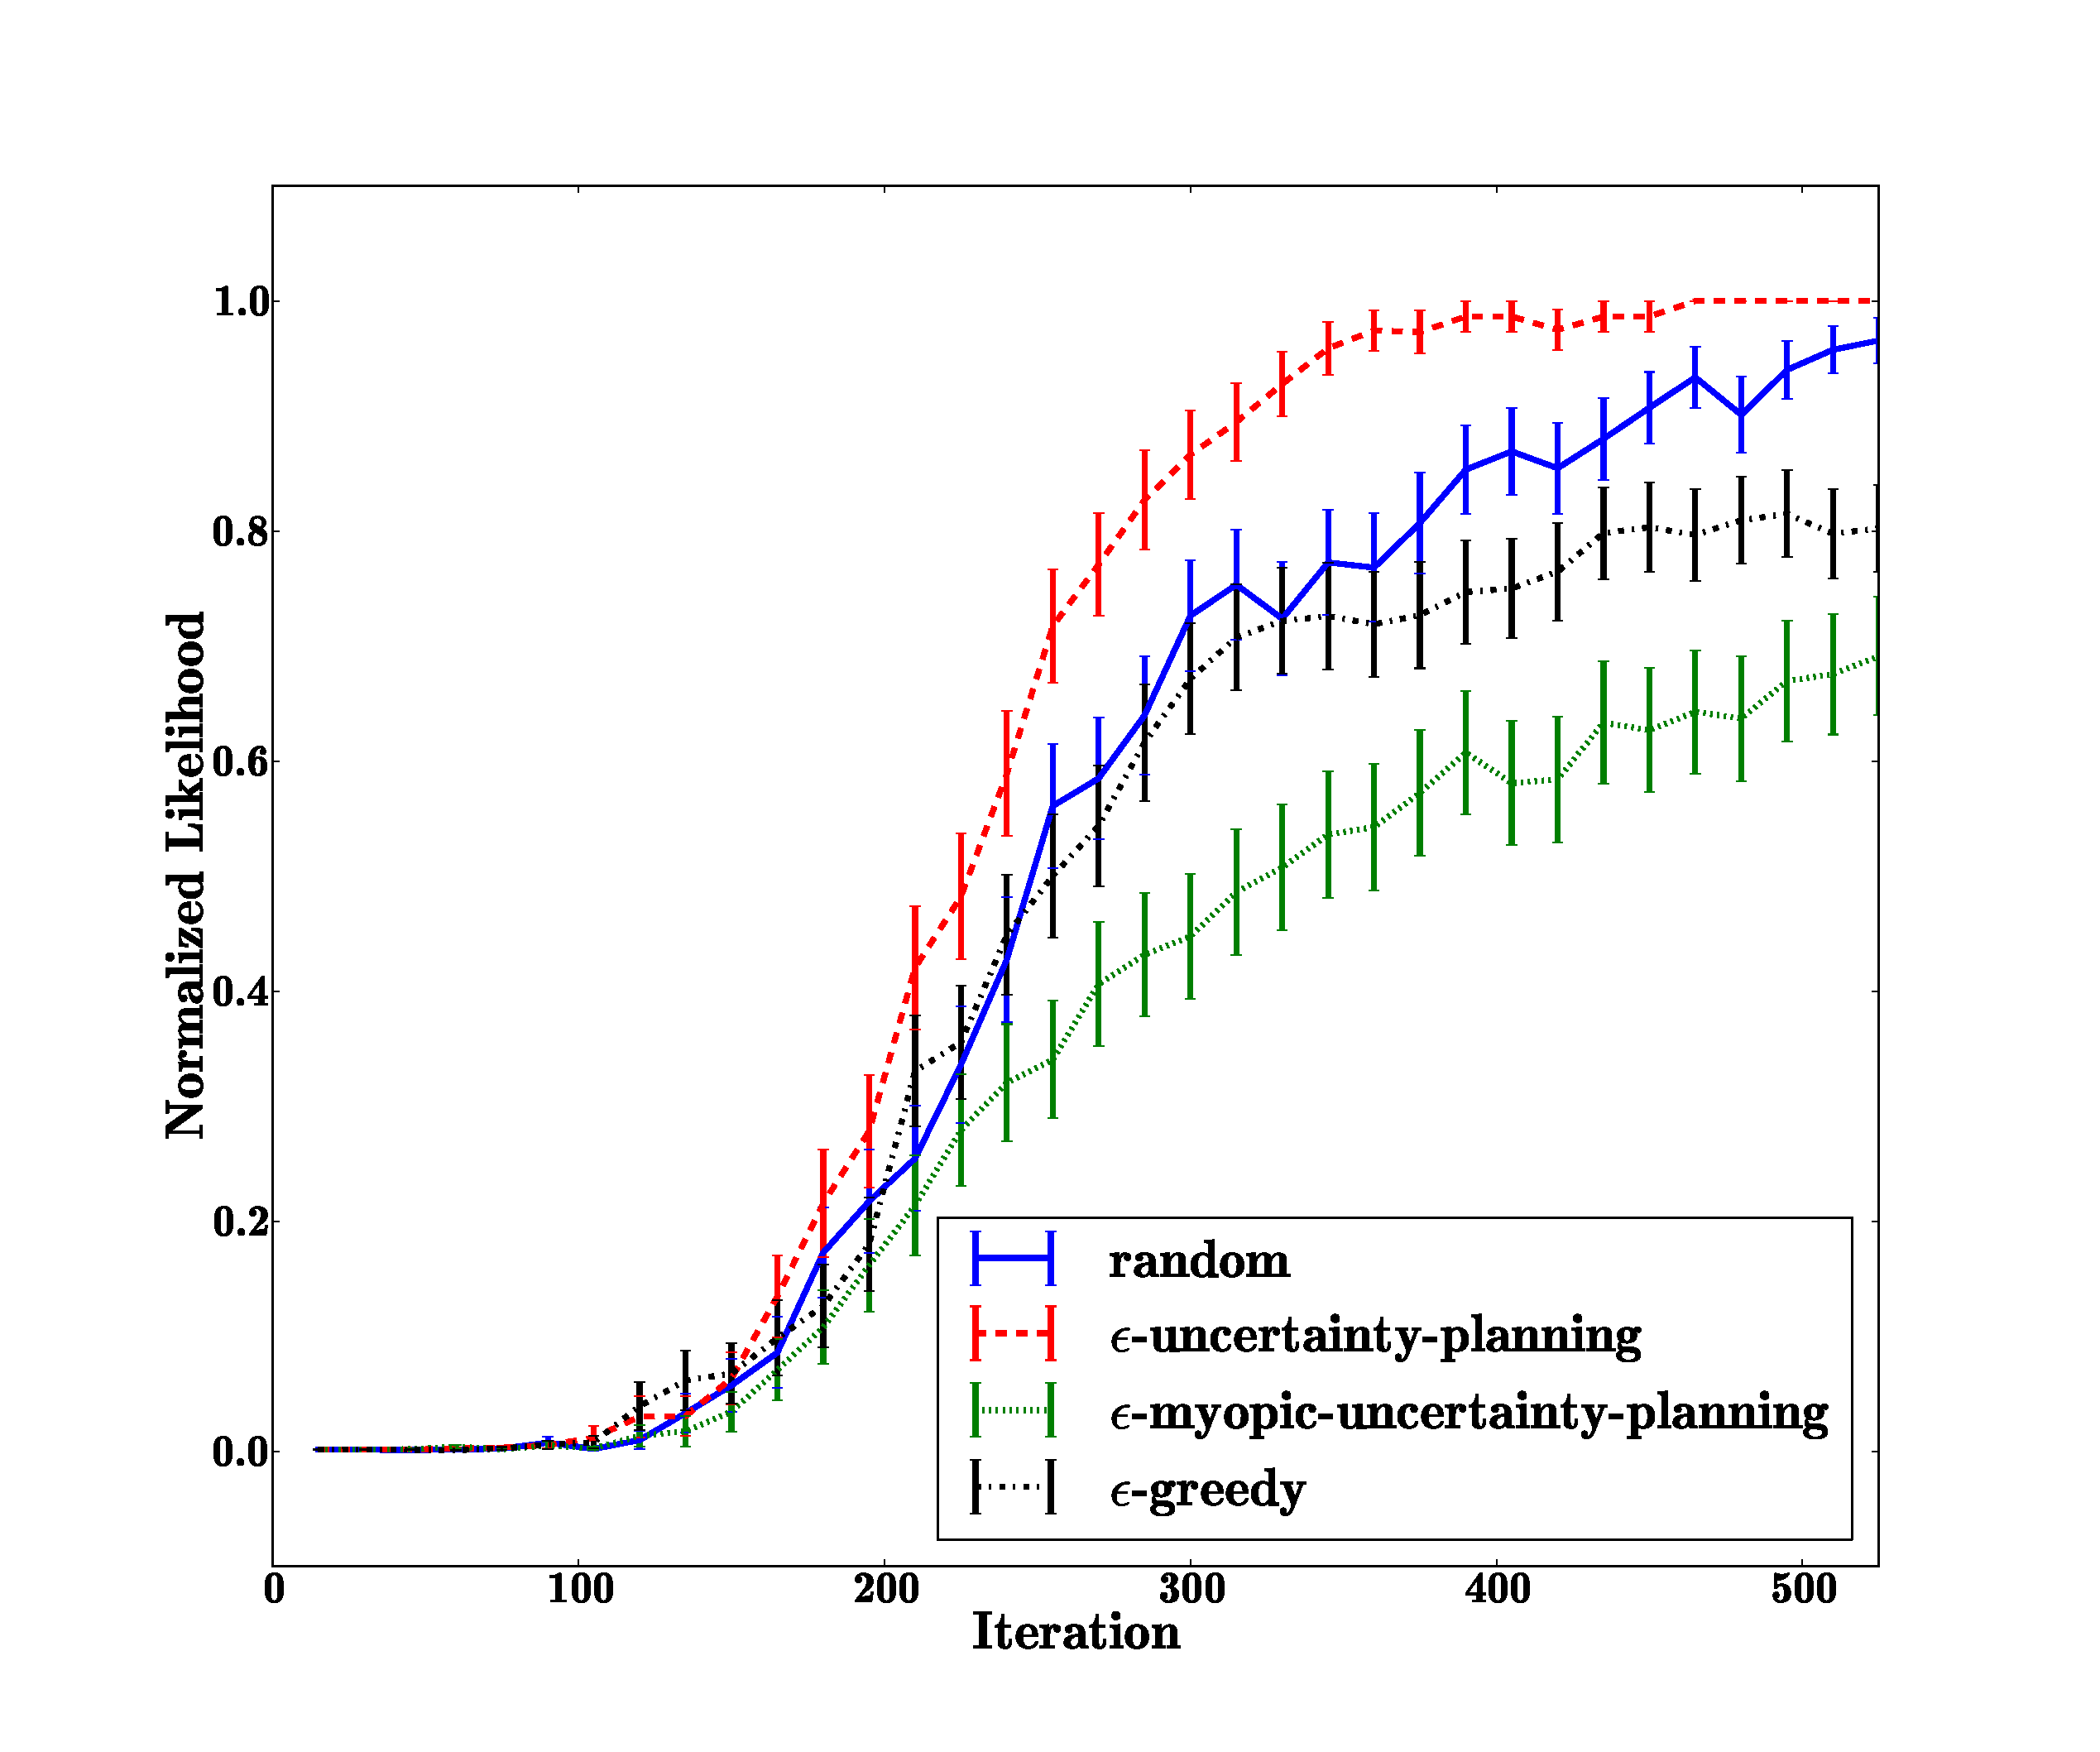
\includegraphics[width=\plotsize\columnwidth]{\imgpath/continuous_state/continuous}
  \caption{Taught hypothesis normalized likelihood evolution (mean + standard error) thought iteration using a Gaussian classifier. Comparison of different exploration strategies. Uncertainty based exploration method, which plan on the long term, performs significantly better on average.}
  \label{fig:continuousstateRmax}
\end{figure}

These results show that our algorithm can learn a task in a continuous world from unlabeled and noisy instructions whose possible meanings are both feedback and guidance and 10 percent of the instructions were teaching mistakes. The uncertainty based planning strategy outperforms random action selection. Interestingly, myopic uncertainty based strategy, which is also based on our uncertainty measure, is not efficient. This result illustrates that, when considering the agent as not being able to teleport, a long term planning approach is more suited to explore efficiently the state space than a short term vision by selecting the next action with higher immediate reward, i.e. higher uncertainty. 

% Finally $\epsilon$-greedy performs less efficiently than in the first setup. This is due to the properties of our new set of hypothesis where many hypothesis shared an identical positive reward area but have different puddle zone.

Figure~\ref{fig:continuousstateUncertaintyMap} shows the evolution of the estimated uncertainty map for one run of the experiment. For each uncertainty map, the agent plans its actions to reach a maximal uncertainty region. The maximum uncertainty value decreases as the agent is correctly estimating the task.

\begin{figure}[!htbp]
  \centering
      \begin{subfigure}[b]{0.35\columnwidth}
          \centering
          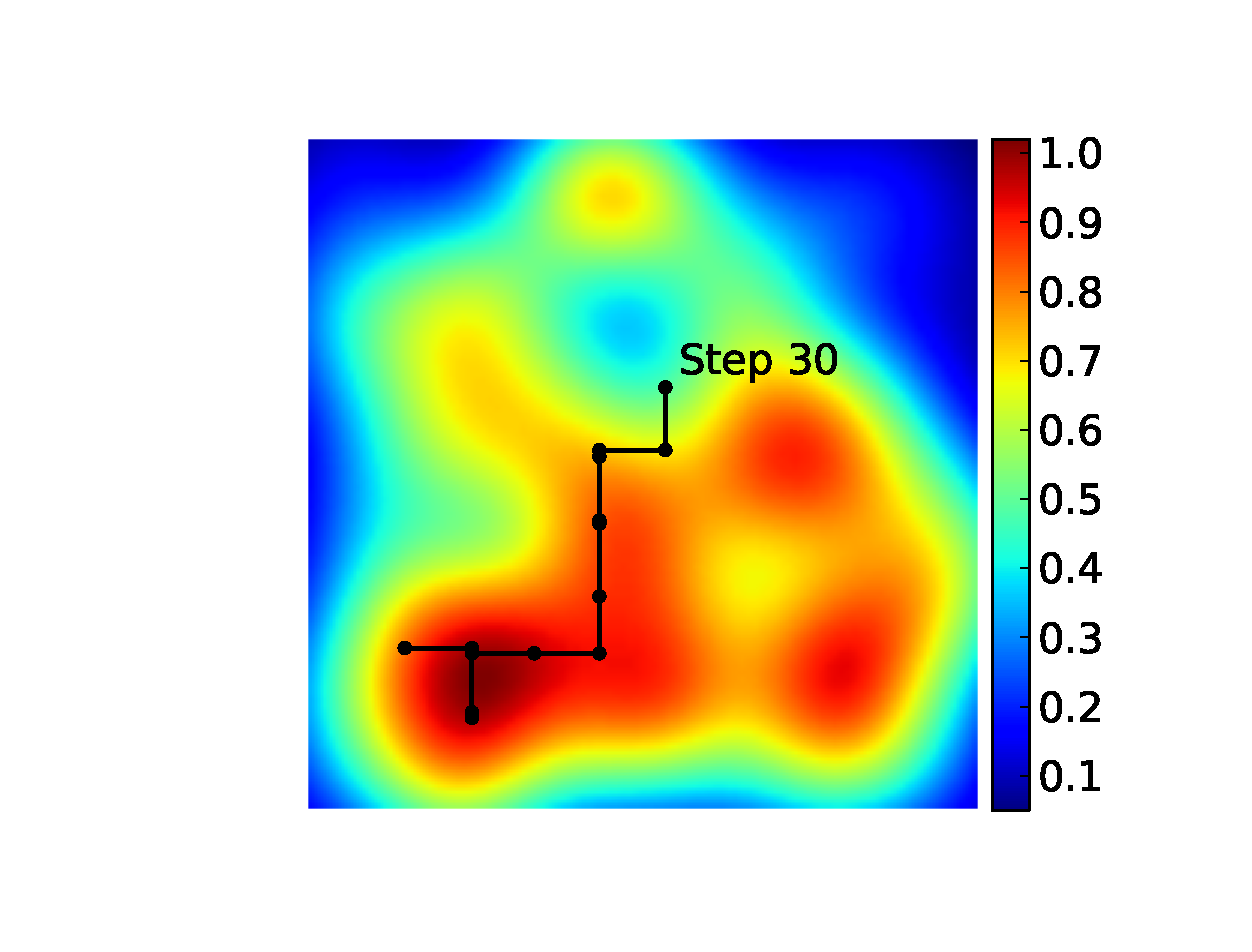
\includegraphics[trim=5cm 1.5cm 1.5cm 1.5cm, clip=true, width=\columnwidth]{\imgpath/continuous_state/30}
          \caption{After 30 iterations.}
          \label{fig:30}
      \end{subfigure}
      \begin{subfigure}[b]{0.35\columnwidth}
          \centering
          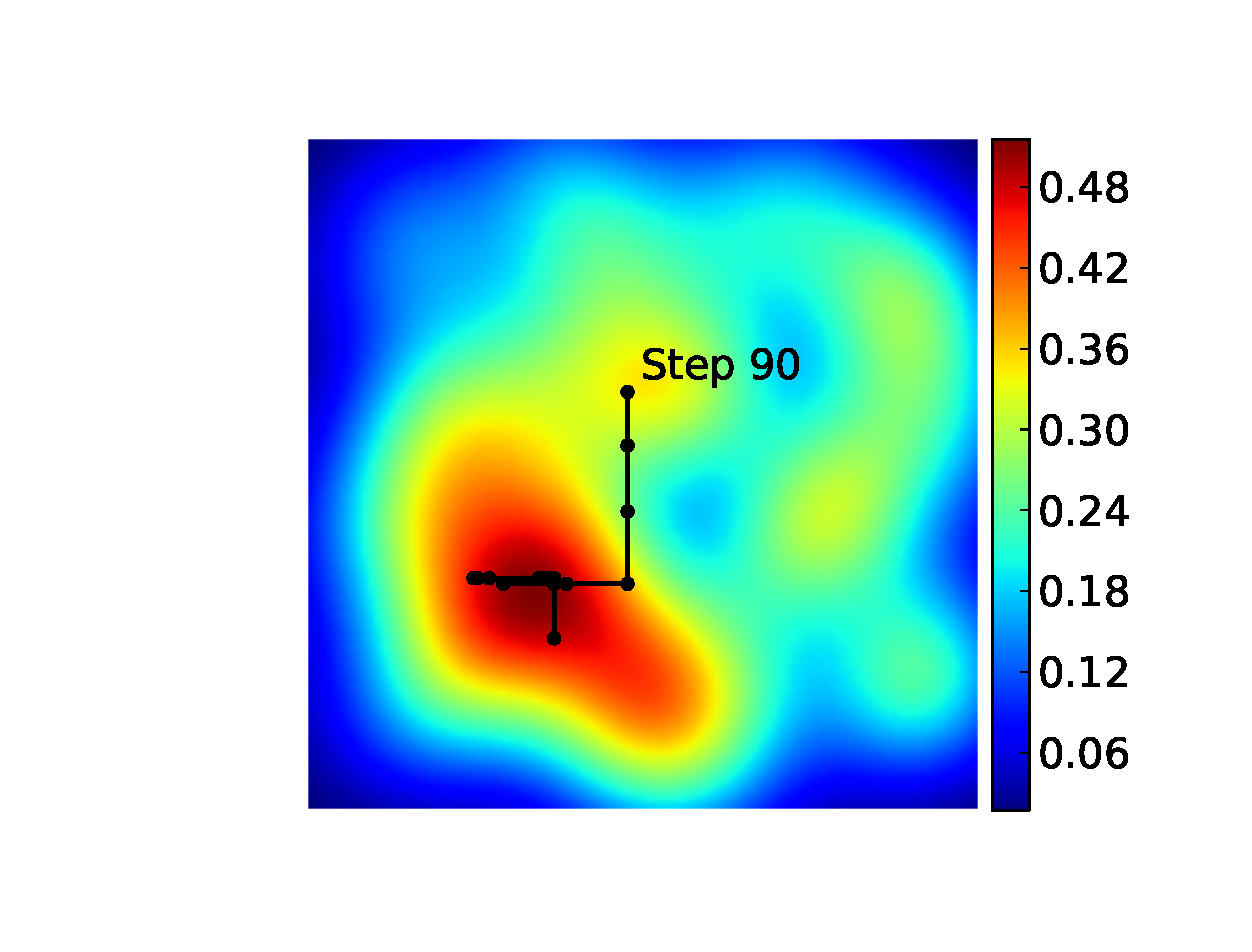
\includegraphics[trim=5cm 1.5cm 1.5cm 1.5cm, clip=true, width=\columnwidth]{\imgpath/continuous_state/90}
          \caption{After 90 iterations.}
          \label{fig:90}
      \end{subfigure}\\
      \begin{subfigure}[b]{0.35\columnwidth}
          \centering
          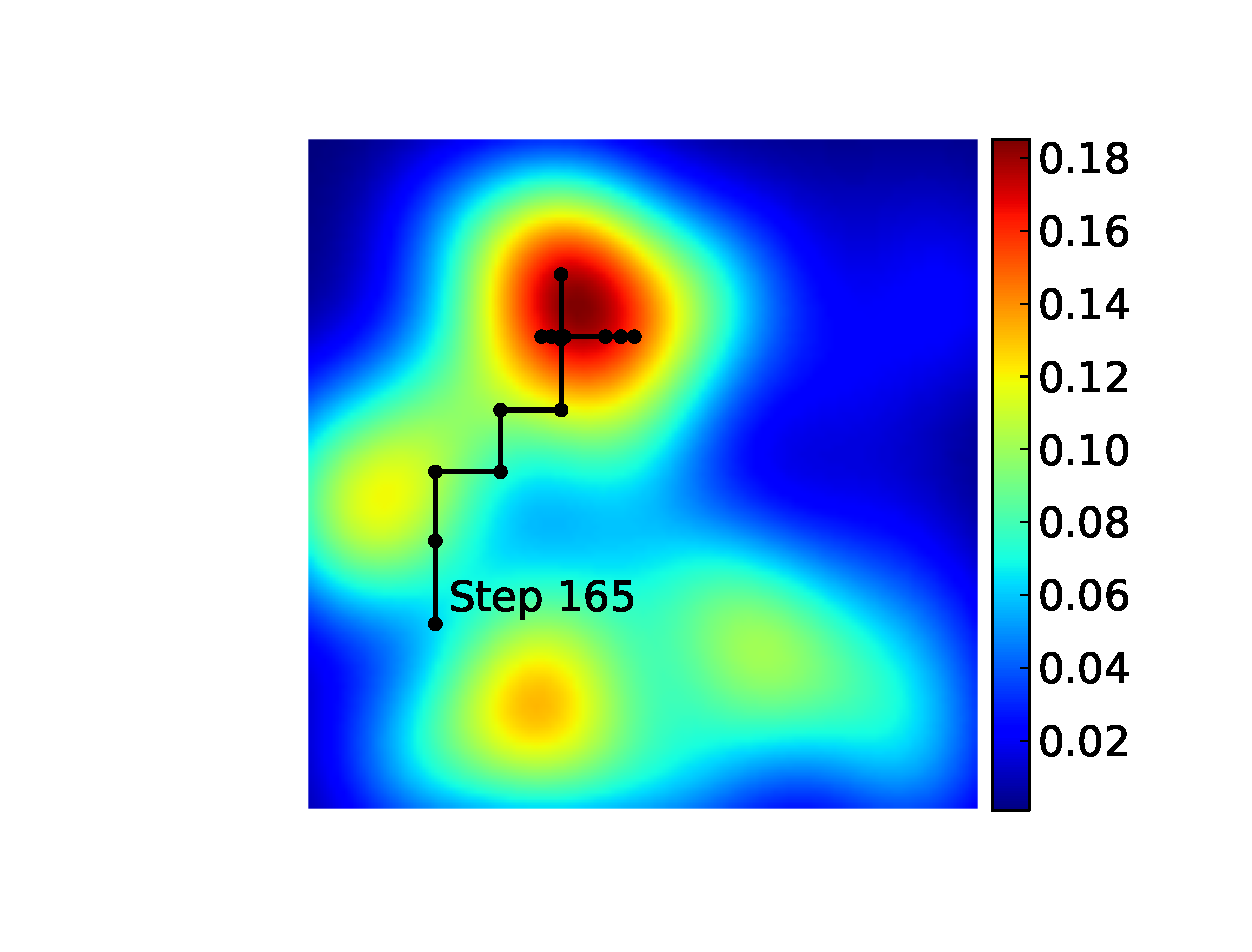
\includegraphics[trim=5cm 1.5cm 1.5cm 1.5cm, clip=true, width=\columnwidth]{\imgpath/continuous_state/160}
          \caption{After 165 iterations.}
          \label{fig:165}
      \end{subfigure}
      \begin{subfigure}[b]{0.35\columnwidth}
          \centering
          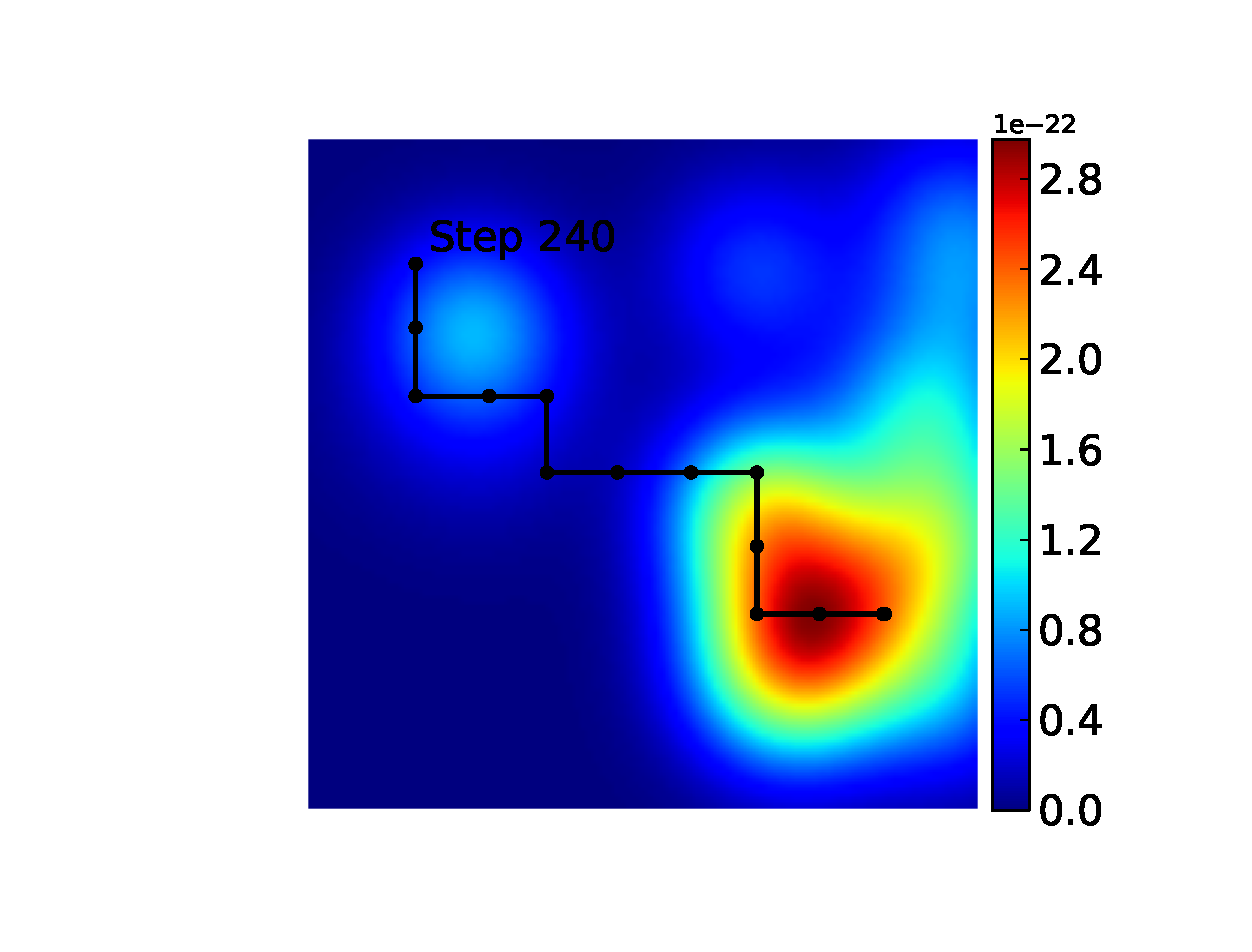
\includegraphics[trim=5cm 1.5cm 1.5cm 1.5cm, clip=true, width=\columnwidth]{\imgpath/continuous_state/240}
          \caption{After 240 iterations.}
          \label{fig:240}
      \end{subfigure}\\
      \begin{subfigure}[b]{0.25\columnwidth}
          \centering
          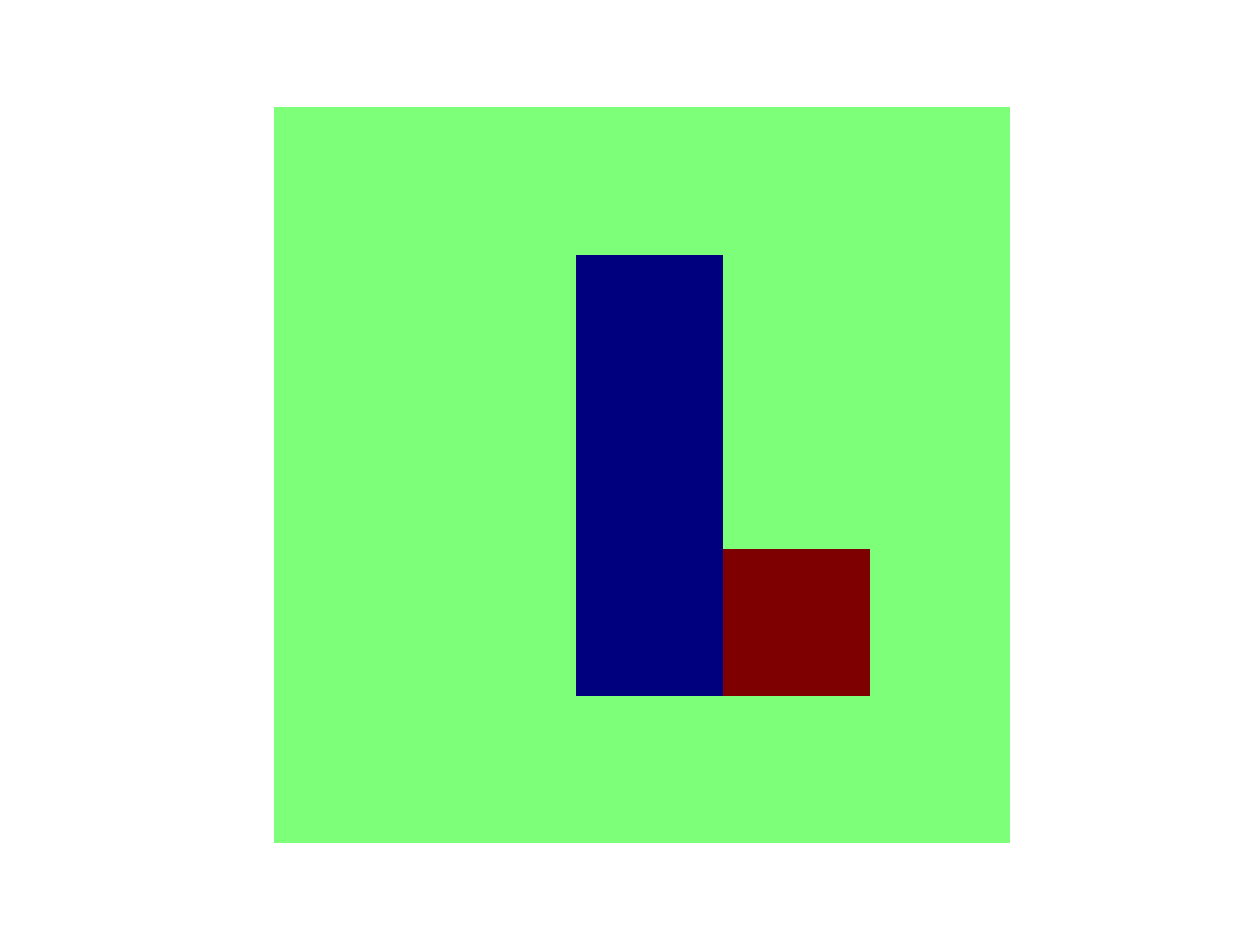
\includegraphics[trim=4cm 1cm 3.5cm 1cm, clip=true, width=\columnwidth]{\imgpath/continuous_state/puddle}     
          \caption{Puddle world used by the teacher.}
          \label{fig:puddle}
      \end{subfigure}
      \begin{subfigure}[t]{0.45\columnwidth}
          \centering
          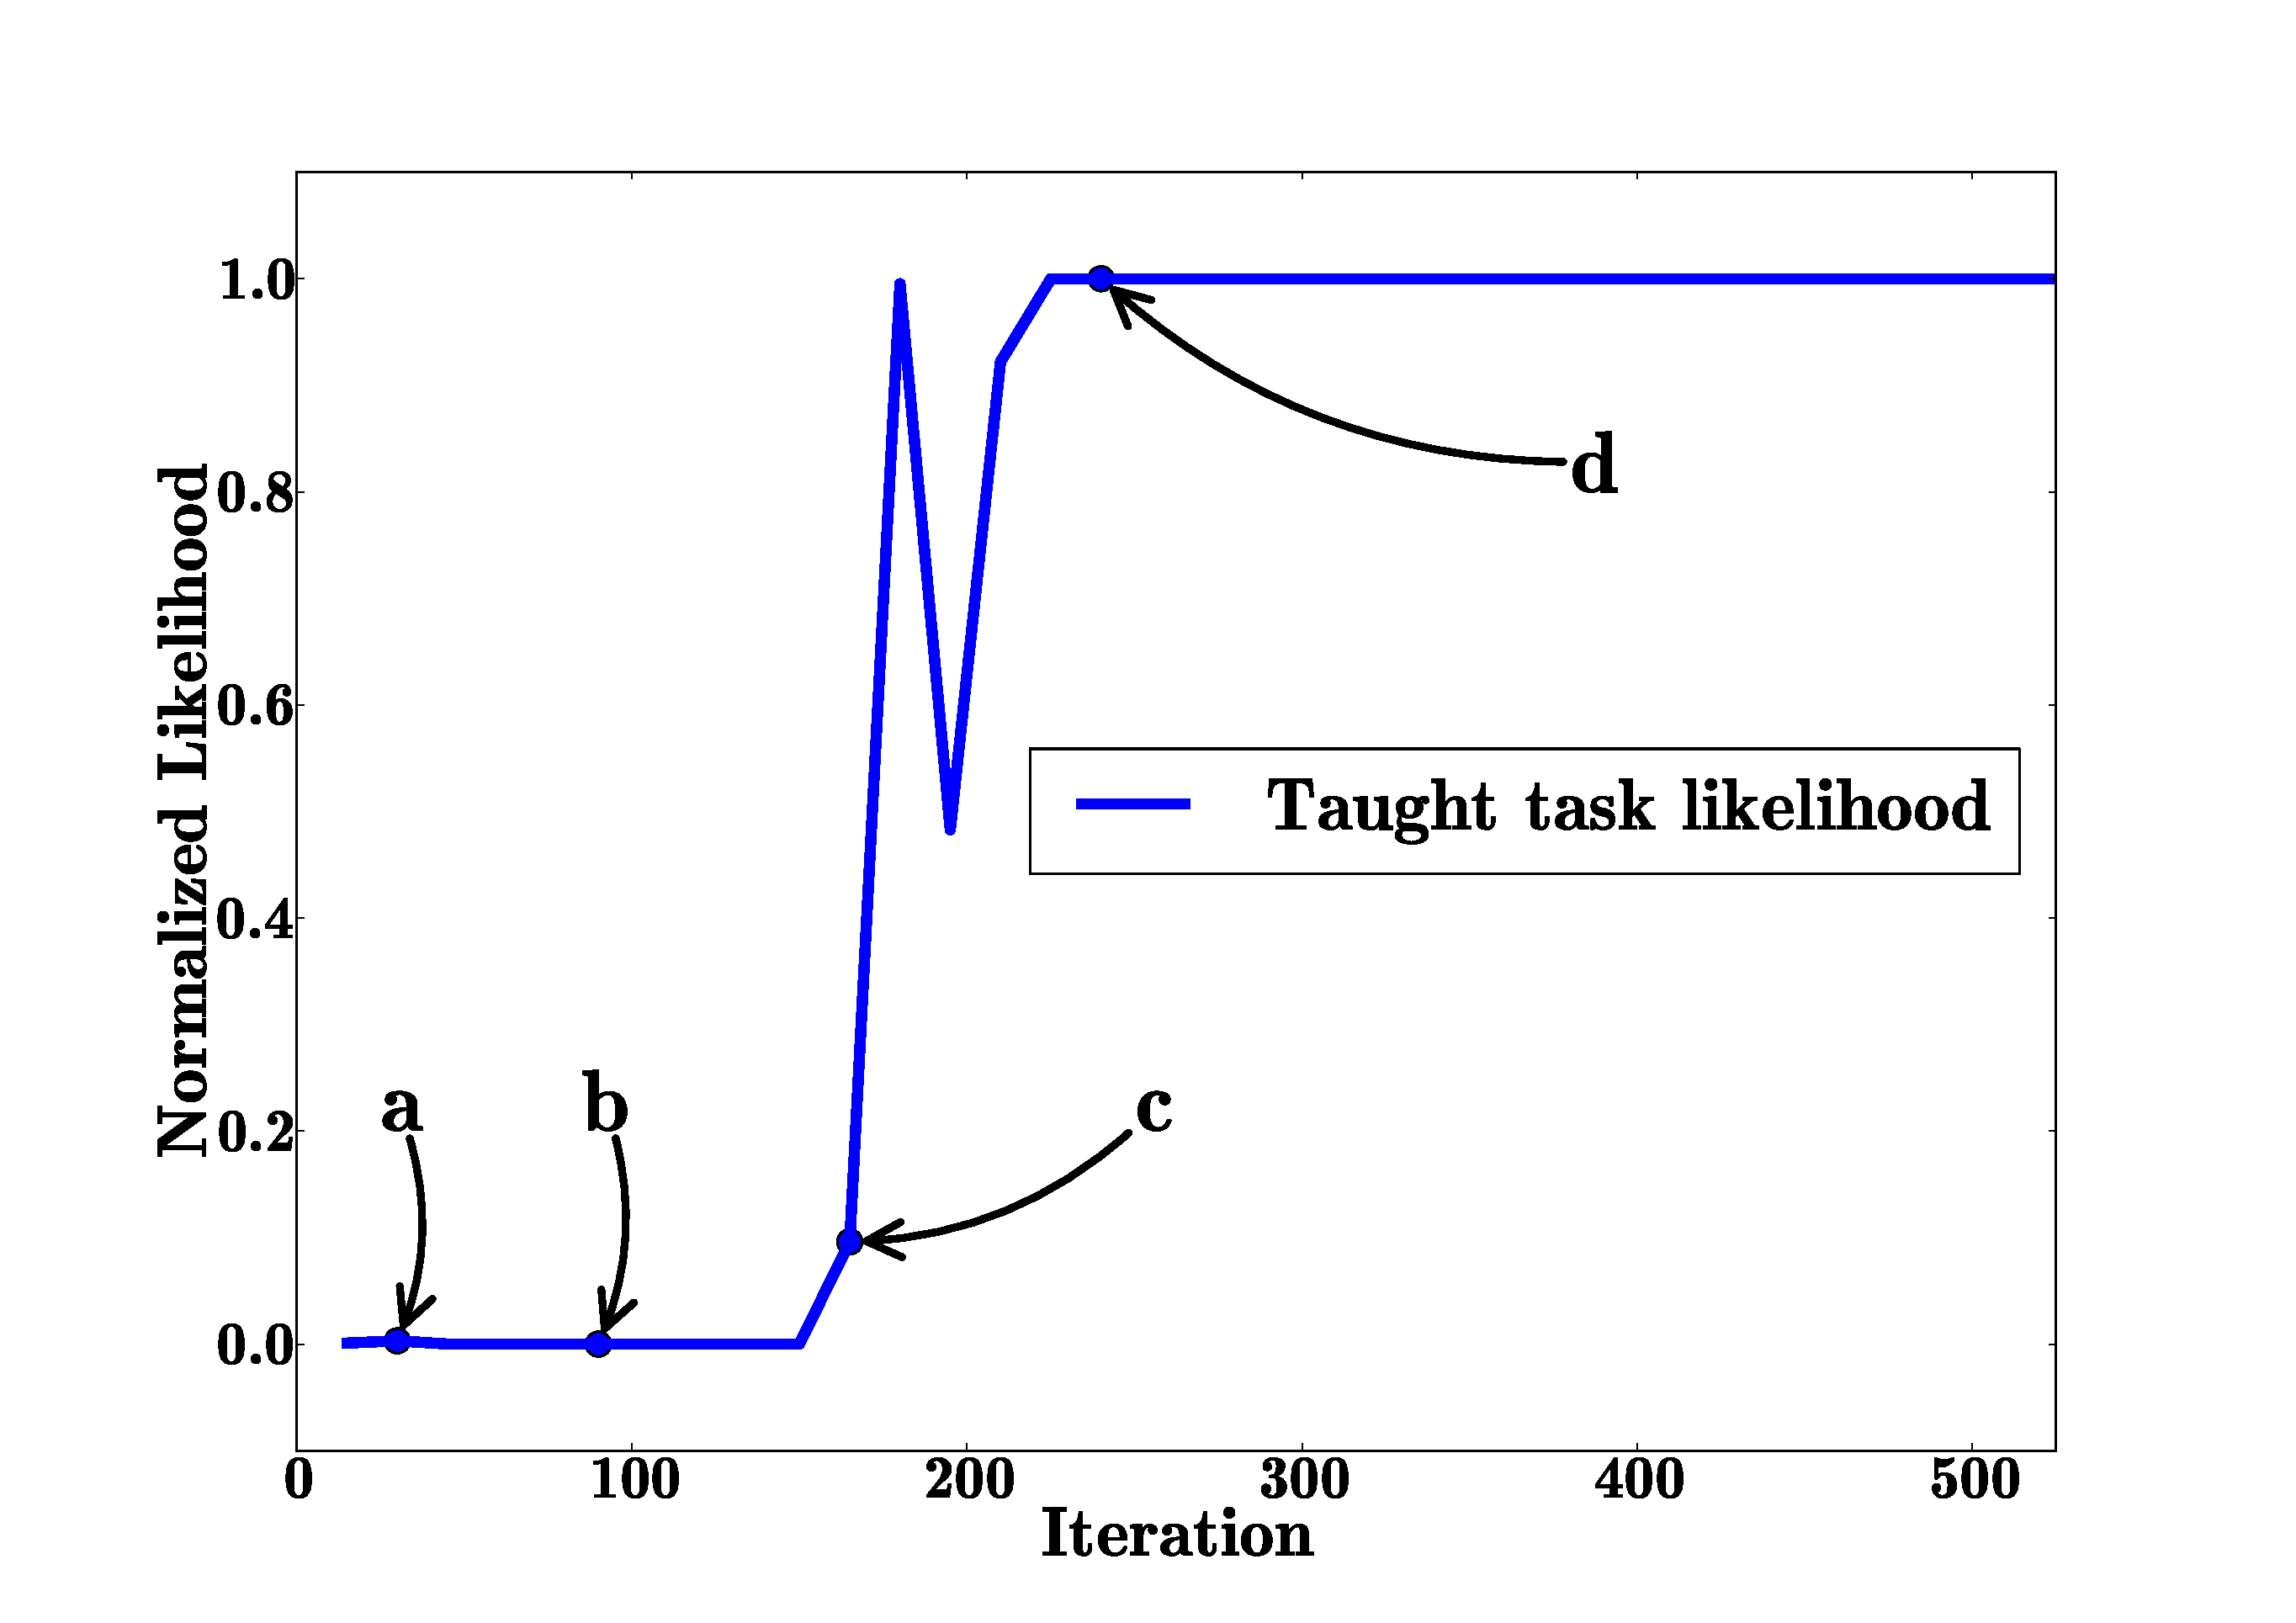
\includegraphics[trim=2cm 1cm 3cm 2cm, clip=true, width=\columnwidth]{\imgpath/continuous_state/evo}
          \caption{Taught hypothesis normalized likelihood evolution.}
          \label{fig:evo}
      \end{subfigure}
        
  \caption{Log Uncertainty maps after a) 30, b) 90, c) 165 and d) 240 iterations. e) shows the puddle world chosen by the teacher and f) shows the learning progress and the frame associated to each of the uncertainty map. In order to display the differences between log values, we bounded the color map between -5 and 0, which correspond to uncertainty values between 0.0067 and 1. Some log values, especially for d), are lower than -5 and are displayed in the same color as -5. Best shown in color.}
  \label{fig:continuousstateUncertaintyMap}
\end{figure}

\subsection{Discussion}

We have shown how our algorithm could be applied to continuous state domains and seen that, given the interaction frame considered, our algorithm only needs to have access to the optimal policies associated to each task to be able to interpret a signal. Therefore any method that allow to compute a policy for continuous domains could be used. The only problem is then related to the computational cost of those methods than to the formalism of this work. We will see in next section that, for some specific frames and worlds, it is not always needed for the robot to know the optimal policies to interpret the teaching signals from the human, which can considerably reduce the computational cost of running our algorithm.
% %!TEX root = ../../thesis.tex

\section{Continuous set of hypothesis}
\label{chapter:limitations:continoushypothesis}

\question{How to leverage from the finite set of hypothesis constraint?}


In order to make the learning problem tractable, it was assumed that the robot learner knows that the task to be learnt can be approximated by one task among a pre-defined set of tasks. Indeed, without constraining the space of possible tasks, an infinite number of task may explain the particular teaching data received by the robot. In practice, the number of pre-defined tasks in the experiment was still relatively large, allowing a certain level of flexibility. Yet, it would be highly desirable to extend the possibility to deal with continuous task representation, allowing potentially infinite spaces of tasks. 

A potential avenue to address this is to constrain search through a combination of regularization and particle filter approaches. In the following of this section, we present a simple particle filter based algorithm that allow an agent to identify a task from unlabeled instruction and considering an infinite set of hypothesis. The agent evolve in a 2 dimensional continuous state and should identify which one of the infinite amount of possible state it should reach.

\subsection{World and task}

We consider an agent living in a 2 dimensional continuous space bounded between 0 and 1 in both dimension. A teacher is providing indication about the orientation of the goal state compared to the robot state by drawing some patterns on a tablet. Those direction can only be selected among of the four cardinal directions that are the directions of north, east, south, and west. The teacher wants the robot to reach a particular state, that can be any position in the continuous 2 dimensional space. The robot is able to teleport itself to any location of the space to receive a new indication.

We still consider a strong a priori knowledge on the space of task, which is that there is only one goal state. This is a very strong a priori regularization on the complexity of the problem. Considering there could be several goal positions, depending for example on the current position of the agent, would increase dramatically the search space; it would then be likely that many hypothesis of different complexity would explain perfectly the observed data. In such case a rule for regularizing the hypothesize task solution would be needed.

\subsection{Finger movements datasets}

We will present results using two different datasets made of finger movements performed on a tablet. 

Our first dataset shown in Figure~\ref{fig:fingerdatasetdirection} is build from a user generating directional trajectories starting from the center of the tablet and going toward the edges of the tablet. We considered four different movement, one toward each edges, representing the four cardinal directions that are the directions of north, east, south, and west. 

\begin{figure}[!ht]
\centering
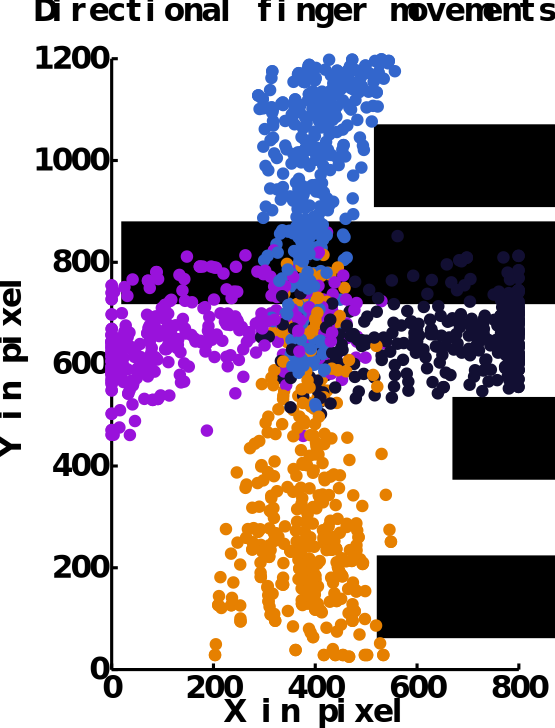
\includegraphics[width=\signalwidth\columnwidth]{\visualspdf/worlds_and_datasets/finger_signals_color.pdf}
\caption{N}
\label{fig:fingerdatasetdirection}
\end{figure} 

Our second dataset shown in Figure~\ref{fig:fingerdatasetsigns} is build from a user drawing The cardinal letters (N, S, W, and E) in the middle of the tablet.

\begin{figure}[!ht]
\centering
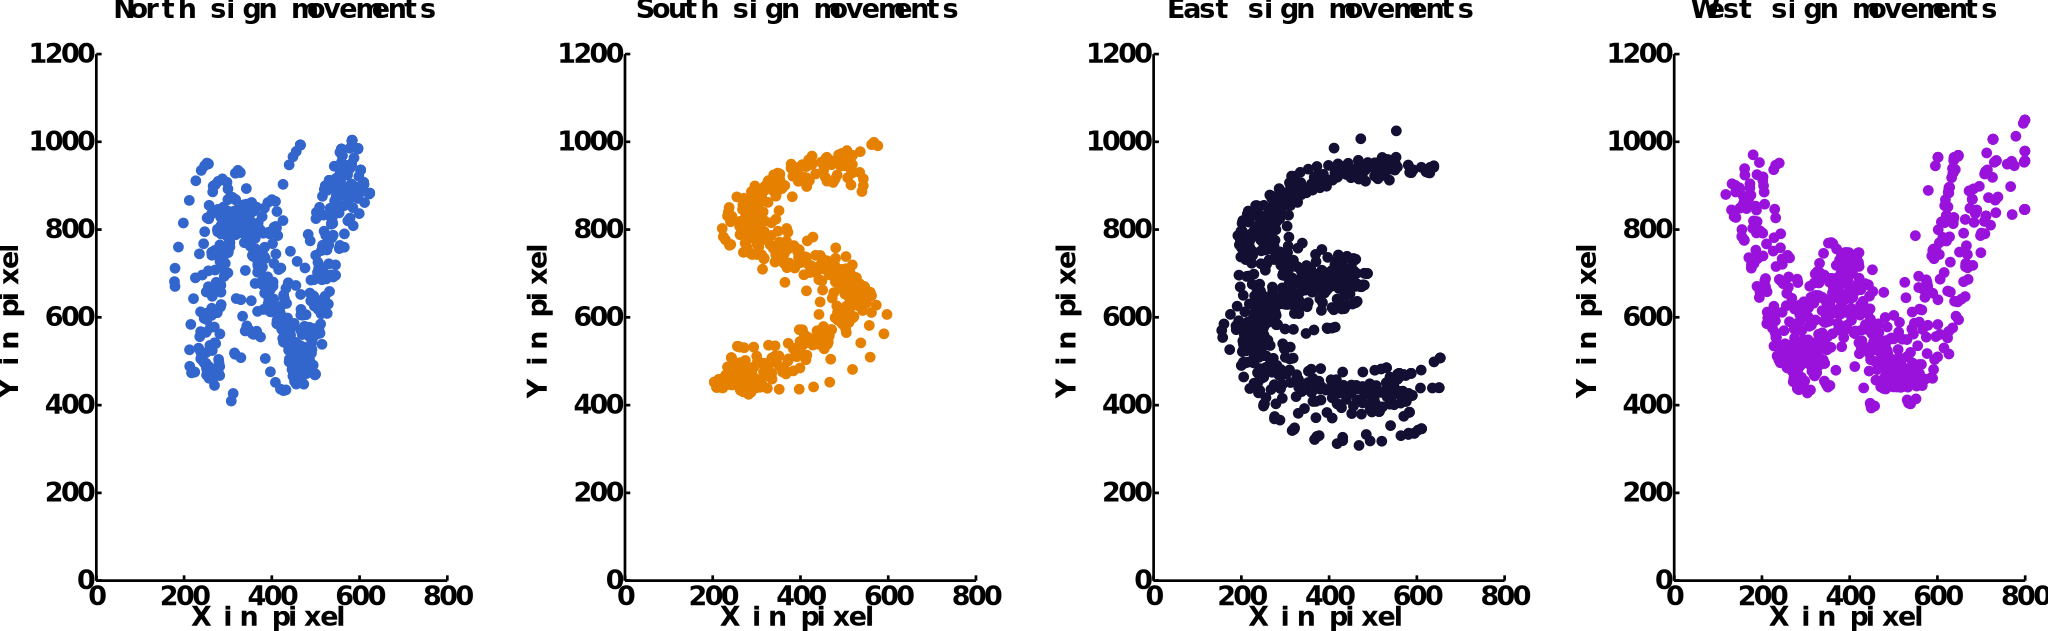
\includegraphics[width=\columnwidth]{\visualspdf/worlds_and_datasets/finger_signals_color_signs.pdf}
\caption{N}
\label{fig:fingerdatasetsigns}
\end{figure} 

To represent those trajectories, our feature vector is composed of 11 dimensions, where dimensions encodes:
\begin{itemize}
   \item The start X and Y positions (2 features)
   \item The end X and Y positions (2 features)
   \item The delta position between start and end position for X and Y coordinate (2 features)
   \item The median X and Y positions (2 features)
   \item The distance between start and end position (1 feature)
   \item The total distance traveled by the finger (1 feature)
   \item The average speed of the finger (1 feature)
\end{itemize}

Using this representation we achieve 100 percent accuracy on the directional movements dataset and 99 percent accuracy on the cardinal signs dataset, using a simple Gaussian classifier with one Gaussian per class.

We remind that the direction of shape of each movement has no a priori meaning for the robot. For example, in our simulation we may use the ``W'' sign signals to mean the goal state is north to the agent position.


\subsection{Evaluating task likelihood}

As there is an infinity of possible goal state, the agent can not estimate the probability of all possible task in parallel. Therefore we will sample a finite number of task at each step and compute a likelihood value for each of those task. Then, given the ranking between them, we will keep some of the best one and sample a bunch of new ones, more details are provided in next subsection~\ref{chapter:limitations:continoushypothesis:particlefilter}.

Our algorithm, as presented so far, was cumulatively accumulating evidence for each task and updated the likelihood of each task on a step by step basis. However for this experiment, as we the task hypothesis are changing step after step, we can not update the likelihood of each task on a step by step basis, as described in Equation~\ref{eq:matchingfiltercrossvalidation}. This approach allowed us to reduce the computational cost of our algorithm so as to be able to run our experiments in a reasonable amount of time. A possible option would be to use Equation~\ref{eq:matchingcrossvalidation}, but we would have to train a huge amount of classifier each step (100000 classifiers after 200 steps in our experiments).

We selected an other option which rely on sampling different classifier from a meta-classifier, which allow us to generate classifiers at a low computational cost. Then given many classifiers for each task, we will compare the likelihood predicted by those classifiers and rank the task by a statistical test on the classifier evaluation. We describe each step of this process in the following paragraph.

The first step is to compute a ``meta'' model which encodes a distribution of probability on the classifier parameters, i.e. which encodes a probability distribution over the mean and covariance of each class. To do so, and given that we are using multivariate normal distribution, we use a noninformative (Jeffrey's) prior \cite{gelman2003bayesian} to estimate the probability distribution over the means and covariances:

\begin{eqnarray}
p(\mu_l|D) & = & t_{n-d}(\mu| \bar{x}_l, \frac{S_l}{n(n-d)})
\label{eq:jeffreysmean}
\end{eqnarray}

\begin{eqnarray}
p(\Sigma_l|D) & = & IW_{n-1}(\Sigma_l | S_l)
\label{eq:jeffreyscov}
\end{eqnarray}

where $\bar{x}_l$ and $\S_l$ respectively represents the ML estimates of the mean and covariance for each class $l$ based on the dataset $D$, $n$ is the number of signals, and $d$ is the dimensionality of a signal feature vector.
$\mu_l$ and $\Sigma_l$ are the posterior probability estimate of the mean and covariance given the noninformative prior. $IW$ denotes an Inverse Wishart function which is the multidimensional generalization of the inverse Gamma, it represents a probability distribution on covariance matrix.

This ``meta'' model encodes the distribution of probability on the classifier parameters. Given this model we can sample, for very low computational cost, a multitude of possible QDA classifiers by sampling a mean and covariance for each class. And the more we have data to fit our model, the less uncertainty remains and the less variability will be observed in the generated classifiers. In our experiment we will sampled 20 classifiers per task.

\todo{text here}


Note that it would seem more straightforward to directly compute the marginal probability distribution of Equation~\ref{eq:prior} which integrates over the all distribution of parameters; and use this for our likelihood estimates of Equation~\ref{eq:matchingoverfitting}. Here we tried to get a measure of confidence on top of our likelihood estimates. This is why we generate several classifiers, test their performances and measure the probability that one set of classifiers is on average better that an other set of classifiers. To do so we model the distribution of performances of a set of classifiers by a normal distribution; and compute the probability that a sample drawn from the distribution associated to one set of classifiers has higher value than one drawn from the distribution associated the an other set of classifiers.

\subsection{Task hypothesis selection and generation}
\label{chapter:limitations:continoushypothesis:particlefilter}

As there is an infinity of possible goal state, the agent can not estimate the probability of all possible task in parallel. Therefore, as described in previous subsection, we sample a finite number of task at each step and compute a confidence measure for each of those task. Given the ranking between them, we will keep some of the best one and sample a bunch of new ones.

\todo{cite particle filtrer}

There is many parameters that will influence the performance of such an algorithm. We can change the number of task sampled, the criteria for selecting the task(s) that stay in the pool from one step to another, and we can change the method used to sample new task. 

As this is an exploratory experiment, we will restrict our analysis to the influence of the method used to resample the pool of task hypothesis and consider either a random or an active strategy. In practice, we will consider a pool of 50 hypothesis. Each step, we will keep the best hypothesis from the pool and replace the 49 others using one of the sampling strategies define next.

The random generation of task simply keeps the best hypothesis and generate 49 new tasks hypothesis randomly.

Our active task generation method simply selects new task around the current best task hypothesis. To do so, we create a mixture of Gaussians which define the probability distribution used to sample the new tasks. This mixture model is composed of:
\begin{itemize}
\item  one fixed Gaussian at the center of the state space (i.e. $[0.5, 0.5]$), with a diagonal covariance matrix, where each value on the diagonal is equal to $0.1$, and have an associated weight of $0.2$. This Gaussian, which as quite spread covariance matrix, maintains a level of exploration in the task generation process.
\item a multitude of Gaussians, one at each location of the previous hypothesis positions (i.e. hypothesized task), whose associated weights are proportional to the probability associated to each task. The sum of the weights of those Gaussians behind 0.8, such as the sum of all mixture component weight is 1. All those Gaussians have a diagonal covariance matrix, where each value on the diagonal is equal to $0.01$. For computational purpose, each Gaussian had a minimal weight of $1e^{-6}$.
\end{itemize}
Note that the resulting distribution will be truncated as all the point generated outside of the boundaries of the space (i.e. between 0 and 1 for each dimension) will be translated to the closest position on the boundaries of the state space.


\subsection{Uncertainty based state sampling}

The agent can also control the next state to teleport to. As seen in chapter~\ref{chapter:planning}, actively controlling agent state important can lead to better performances. Indeed the state of the agent influences the signal sent by the teacher. 

We will compare two kind of active sampling, random and an uncertainty based method. The random method simply teleport the agent to a random position in the world. 

The active method rely again on a sampling method. At each step, we generate 1000 states randomly and compute the uncertainty associated to those states using the method describe in chapter~\ref{chapter:planning} by Equation~\ref{eq:planning} and using up to 20 sampled signals from our history of interaction. For the next state, we select, among the 1000 points, the one that as higher uncertainty, and teleport the agent to that state in order to collect the next teaching signal.


\subsection{Results}

We will compare all four combinations of the methods described above \begin{inparaenum}[a)] \item random state and task selection (which we call ``random random''), \item random selection of next state and active task sampling (which we call ``random active''), \item uncertainty based selection of next state and random task selection (which we call ``uncertainty random''), and \item uncertainty based selection of next state and active task sampling (which we call ``uncertainty active''). \end{inparaenum}

We ran 100 simulated experiments for each method and each dataset. Each experiment lasted 200 iteration and started by 12 random steps such as to collect enough point to use Equation~\ref{eq:jeffreysmean}~and~\ref{eq:jeffreyscov} with our 11 dimensional signals.

\paragraph{Distance to goal state}

For each method, we compare the evolution of the distance between the best task hypothesis through iteration (the more probable according to our estimate) and the goal state (see Figure~\ref{fig:continuoustaskdistevolution}).

\begin{figure}[!ht]
\centering
\includegraphics[width=0.62\columnwidth]{\imgpath/continuous_task/distEvolution.eps}
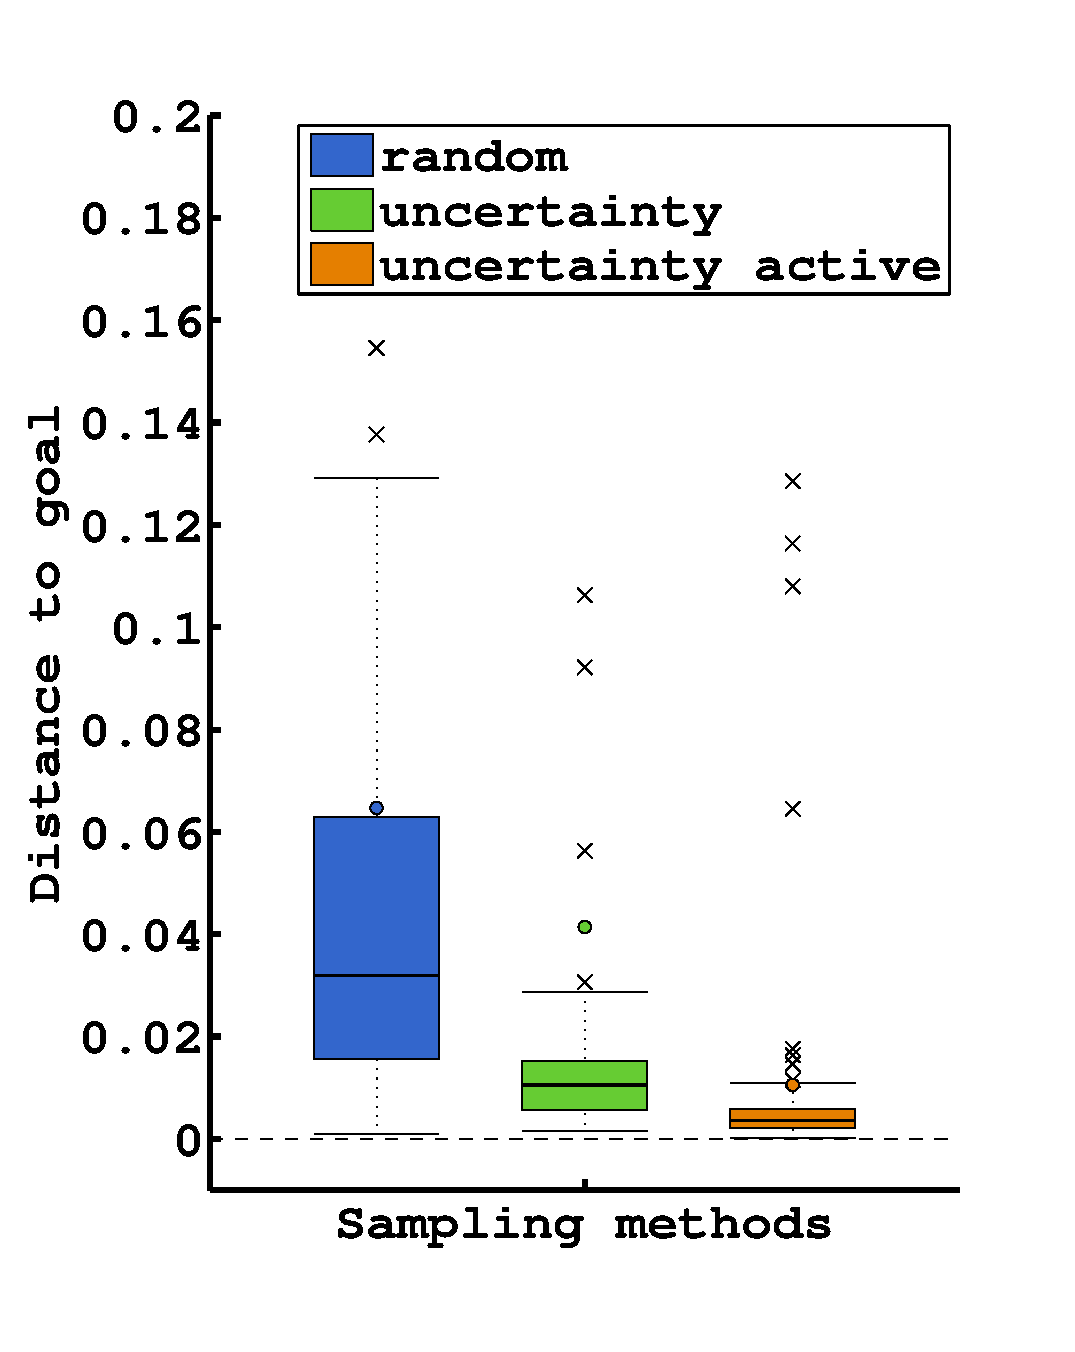
\includegraphics[width=0.37\columnwidth]{\imgpath/continuous_task/endDist.eps}
\caption{Evolution of the distance to target using the directional finger movement dataset shown in Figure~\ref{fig:fingerdatasetdirection}. On the left is the evolution of the distance of the best position hypothesis to the goal position (mean and standard error shown as shaded area). On the right is a box plot of the distance of the best position hypothesis to the goal position at the end of the 200 iterations. Actively sampling new task hypothesis as well as selecting new state based on our uncertainty estimation outperform allow to identify the target position with very high accuracy and low variance. Note that some distant outliers are not shown on the box plots for readability reasons.}
\label{fig:continuoustaskdistevolution}
\end{figure}

Only the combination of actively sampling new task and actively selecting new state based on their relative uncertainty as overall better performance than any other combination of our method. Those two method are complementary, to find a task hypothesis better than our previous best estimates, it is likely that it is close to the current best hypothesis. Our active task sampling method allow to explore close to our previous best estimates. However, now that we have some hypothesis located in a restricted area of the space, we need to sample state in very precise location to be able to differentiate them, which our uncertainty based state selection allow. This explain why using one of the two method alone do not reach the same performances as their combination.

In Figure~\ref{fig:continuoustaskdistevolution} left, we compare the distribution of final distance between our best hypothesis and the true goal position. First note that the important difference between displaying our results in terms of mean and standard error or in terms of a box plot, which shows the median and the 25th and 75th percentile (you can see the mean value as a colored dot). Especially for the ``uncertainty random'' method, the visual impression of the performance of the methods differs. This is due to the outliers, where even a few values far away from the main group of point can ``push'' the mean away, the normal distribution assumption do not hold for presenting our results. In order to statistically compare the efficiency of our methods, we use the Mann-Whitney U-test \cite{mann1947test} which is a nonparametric test for equality of population medians of two independent samples. We will use the one tailed version to specifically test whether one population has greater performances than the other. There is no measurable statistical difference between the ``random random'' and ``random active'' methods ($p = 0.68$). The ``uncertainty random'' performances over ``random random'' ($p<1e^{-10}$) and ``random active'' ($p<1e^{-10}$) are highly significant. As well as the difference between the ``uncertainty active'' and ``uncertainty random'' difference in performance ($p<1e^{-10}$).

The results presented above where obtained using the directional finger movement dataset shown in Figure~\ref{fig:fingerdatasetdirection}. We now demonstrated how the same algorithm could handle different preferences of user finger gesture for cardinal direction indication. To do so we repeat the experiment wit the cardinal sign dataset of Figure~\ref{fig:fingerdatasetsigns}

\paragraph{Task sampling comparison}

\todo{Show the map of sampled task with sampling versus random} 

\paragraph{State sampling comparison}

\todo{Show the end map of sampled state with sampling versus random} 



% %!TEX root = ../../thesis.tex

\section{Interaction frame hypothesis}
\label{chapter:limitations:framehypothesis}

\question{How to relax the assumption that interaction frame is pre-defined and unique?}

Until now we have assumed that the interaction frame, which specifies the details of the interaction between the human and the machine was known. In this section, we considered the case where multiple interaction frames are defined, but only one of them accounts for the interaction between the human and the machine.

% In this frame only the meaning of the signal was unknown. 

\subsection{Illustrations}

We will use a very simple example to illustrate the problem and show computational results. We consider that the agent lives in the line word as defined in chapter~\ref{chapter:lfui::symmetries}, where the agent has access to the ``no move'' action in order to remove the symmetry problem. The agent knowns it should reach either of the two edges of the world, G1 or G2. And the agent knowns that the teacher is providing either feedback or guidance instructions. To handle this new hidden information we will rely again on our interpretation hypothesis process. This time, one hypothesis will be the combination of one task hypothesis and one frame hypothesis. For our simple example, it results in having four hypotheses.

The result of the labeling process is shown in Figure~\ref{fig:multipleframeexplainedfeedback} for a teacher providing feedback instructions according the task G1. The hypothesis that labels the signals according to the task G1 and the feedback frame is the one whose signal-label pairs match better with the underlying structure of the data. Indeed, for the guidance case, the labeling process for hypothesis G1 is always giving a ``left'' label whether or not the agent is moving away or closer to the target, which allows to differentiate between feedback and guidance cases. To differentiate between G1 and G2, the same principle than the one described in chapter~\ref{chapter:lfui::symmetries} applies.

\begin{figure}[!htbp]
\centering
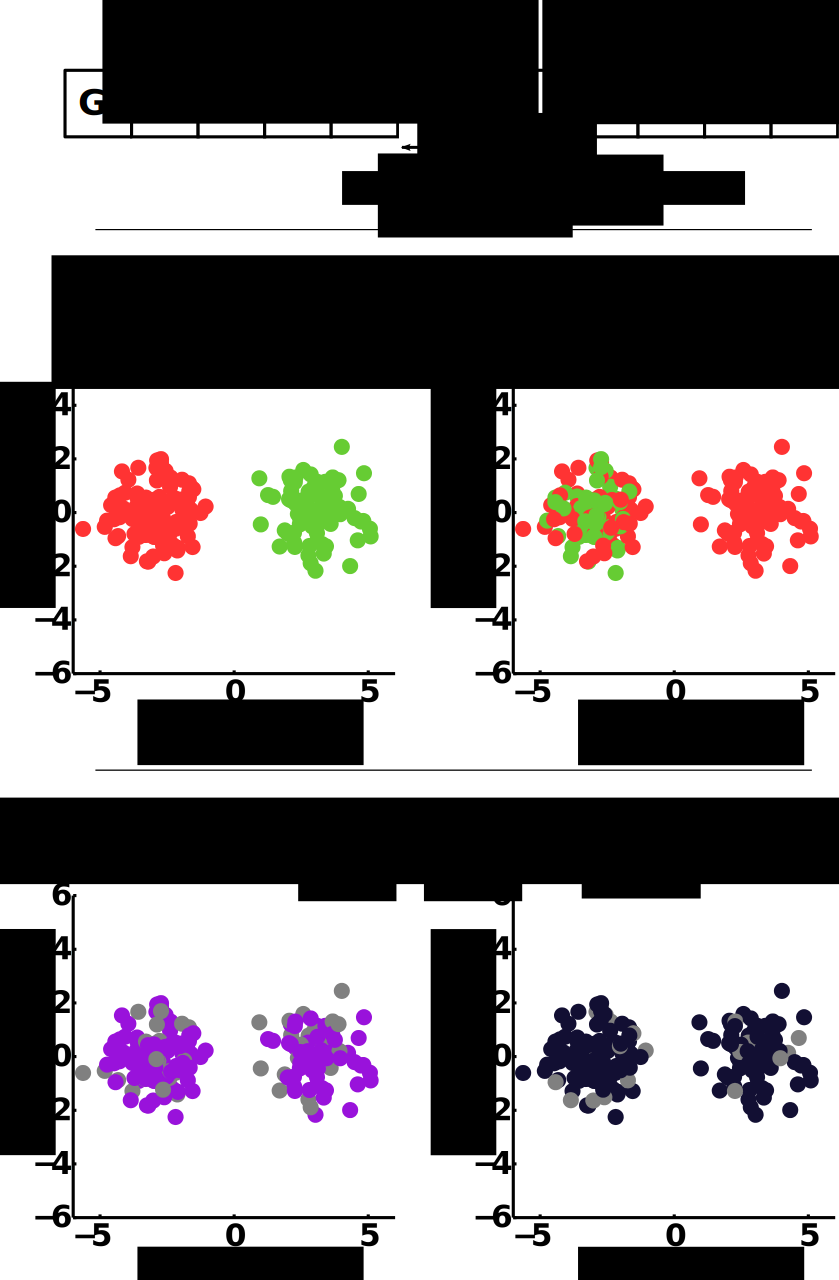
\includegraphics[width=\twoplanningwidth\columnwidth]{\visualspdf/multiple_frame/multiple_frame_feedback.pdf}
\caption{Illustration of the labeling process on both task and interaction frame hypothesis. The agent can perform right, left, or a ``no move'' action. The agent receive feedback on its action in the line word according to G1 . The agent do not known which task (G1 or G2) neither which interaction scheme the teacher is following (feedback or guidance). The result of the labeling process allow to identify the hypothesis on task G1 and feedback frame as the more likely.}
\label{fig:multipleframeexplainedfeedback}
\end{figure} 

Considering now that the teacher is providing guidance instructions according the task G1, the results of the labeling process can be seen in Figure~\ref{fig:multipleframeexplainedguidance}. The same explanation than for Figure~\ref{fig:multipleframeexplainedfeedback} applies. 

\begin{figure}[!htbp]
\centering
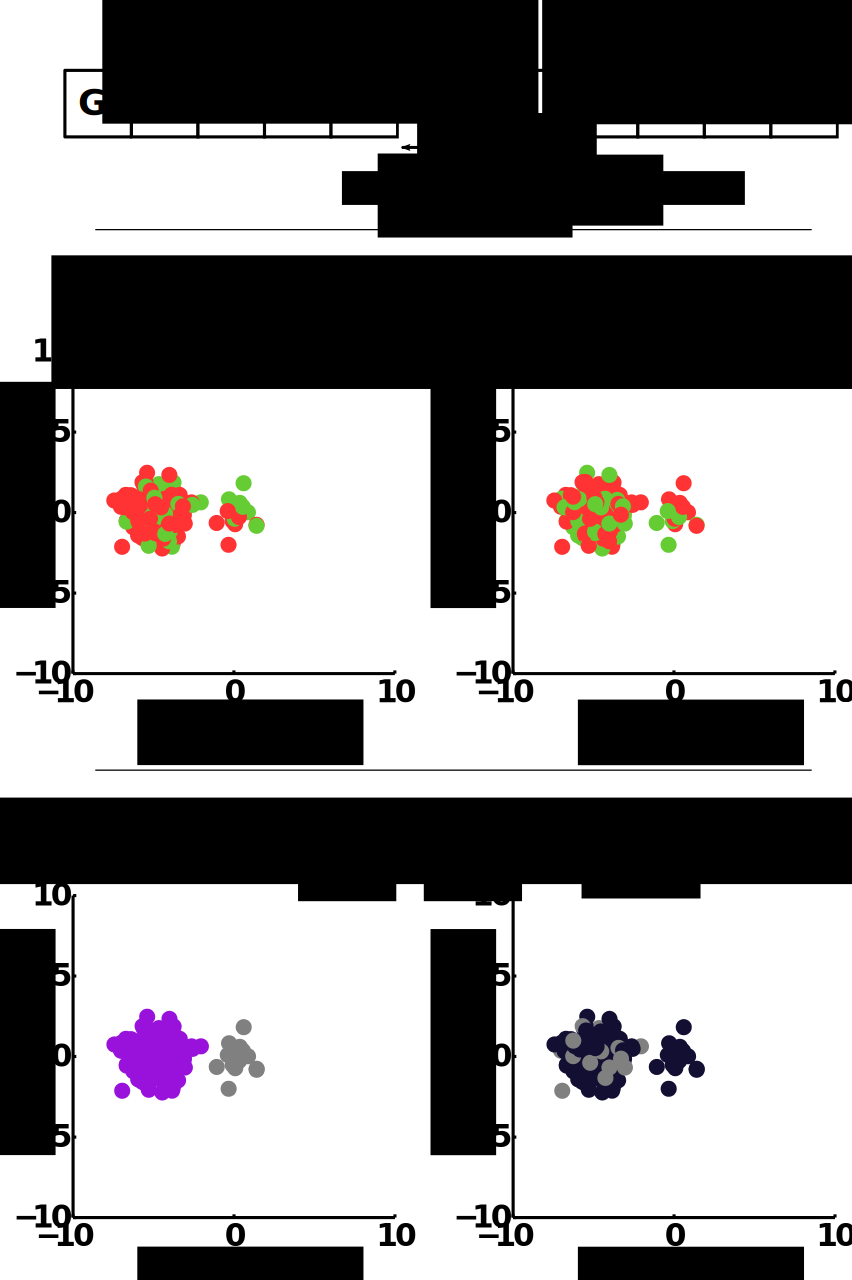
\includegraphics[width=\twoplanningwidth\columnwidth]{\visualspdf/multiple_frame/multiple_frame_guidance.pdf}
\caption{Illustration of the labelling porcess on both task and interaction frame hypothesis. The agent can perform right, left, or a ``no move'' action. The agent receive guidance instruction on its action in the line word according to G1 . The agent do not known which task (G1 or G2) neither which interaction scheme the teacher is following (feedback or guidance). The result of the labeling process allow to identify the hypothesis on task G1 and guidance frame as the more likely.}
\label{fig:multipleframeexplainedguidance}
\end{figure} 

\subsection{Simple experiments}

We now verify that the algorithm works in practice. We consider the same line world scenario as described above. For our experiments, the simulated teacher selects randomly a target (G1 or G2) and an interaction frame (feedback or guidance). The agent is using our uncertainty based planning method. We ran 100 simulations. All other settings were set as for the experiments of chapter~\ref{chapter:planning:method}.

Figure~\ref{fig:multipleframeall} shows the evolution of the probability associated to the correct combination of task and interaction frame (we use the minimum of pairwise normalized likelihood from Equation~\ref{eq:probapairwise} in chapter~\ref{chapter:lfui:confidence}). After 200 steps, all our experiments identified with probability 1 the correct combination of task and interaction frame. 

% In practice, in our previous experiments, we used a confidence threshold of 0.9, under this condition most of our experiments would have identified the task in slighlty more than 50 steps.

\begin{figure}[!htbp]
\centering
\includegraphics[width=\plotsize\columnwidth]{\imgpath/multiple_frame/multiple_frame_all_teacher.eps}
\caption{Evolution of the minimum of pairwise normalized likelihood for the correct hypothesis. After 200 steps, all our experiments identified with probability 1 the correct combination of task and interaction frame. Most of the experiments would have identified the task slighlty more than 50 steps with a confidence threshold of 0.9.}
\label{fig:multipleframeall}
\end{figure} 

We plot in Figure~\ref{fig:multipleframefeedbackvsguidance} the cases where the teacher was using the feedback frame (left) or the guidance frame (right). The performance are similar in both cases.

\begin{figure}[!htbp]
\centering
\includegraphics[width=0.49\columnwidth]{\imgpath/multiple_frame/multiple_frame_feedback_teacher.eps}
\includegraphics[width=0.49\columnwidth]{\imgpath/multiple_frame/multiple_frame_guidance_teacher.eps}
\caption{Evolution of the minimum of pairwise normalized likelihood for the correct hypothesis if the teacher provided feedback (left) or guidance (right) instruction. After 200 steps, all our experiments identified with probability 1 the correct combination of task and interaction frame. Most of the experiments would have identified the task in slightly more than 50 steps with a confidence threshold of 0.9.}
\label{fig:multipleframefeedbackvsguidance}
\end{figure} 


\subsection{Discussion}

Following the interpretation hypothesis method on a combination of task and interaction frame, we can start learning a task from unlabeled instructions and undefined interaction frames. In other words, such system can not only learn the task and the signal to meaning mapping, but also the interaction protocol used by the teacher.

Considering our example in section~\ref{chapter:limitation:continuoushypothesis}, an application this method can be to consider different coordinate system for the cardinal frame. For example, the signals from the teacher can be relative to the true North magnetic pole, to the current position of the user relative to the agent, or relative to the current orientation of the robot. This experiment performed with a real robot, real users, considering a tablet, and different interaction frames has great potential to demonstrate the potential application of this work.

Finally, we note that a particle filter based method (as used in section~\ref{chapter:limitations:continoushypothesis} for dealing with continuous task) could be considered for dealing with a continuous set of interaction frames. For example, in our example of section~\ref{chapter:limitations:continousstate}, we used a parameterized frame that merged feedback and guidance frame (see Equation~\ref{eq:mixedfeedbackguidance}), and introduced a feedback to guidance ratio $\alpha$. By generating, testing, and resampling a set of $\alpha$, i.e. a set of interaction frames, we may be able to learn, not only the task and the signal to meaning mapping, but also the details of the interaction protocol used by the teacher.

 % For example, in the experiment of section~\ref{chapter:limitations:continousstate} we may identify automatically the $\beta$ parameter of Equation~\ref{eq:mixedfeedbackguidance}.
% %!TEX root = ../../thesis.tex

\section{Human in the loop}
\label{chapter:limitations:userstudies}

\question{Do people want to have an open-ended choice about what signal to use? \\ Would they be more efficient?}

Only prerecorded datasets have been used. However, signals may change during the learning. For instance, people can try to adapt themselves to a robot if they believe the latter is not understanding properly. Or, brain signals are sensitive to the protocol, the duration of the experiment or even the percentage of errors made by the agent \cite{chavarriaga2010learning}. To which extend the behavior of our agent changes the properties of the teaching signal? 

Moreover, in real-world applications, users are usually told how to interact with machines. And having a free choice on some details of the interaction may finally become a disadvantage and lower perfomances. Do people want to have an open-ended choice about what signal to use? Would they be more efficient? When is it better to use a calibration procedure?

As we argued in the introduction, the work we presented is a starting point towards forms of adaptive interaction with non-technical users, that we may call fluid interaction learning. While we studied in this thesis properties of learning algorithms that will be needed for such an endeavor, it remains to be shown how they can be integrated within a full real-world human-robot interaction scenario and architecture so that the usability and acceptability of such system can be evaluated. Thus, user studies in particular will be a crucial next step of this work. The improvements described in previous section may be needed to reach acceptable levels of usability.

An interesting direction would be to consider the same experimental setup as the one used in chapter~\ref{chapter:humanexperiment} which allow to seamlessly use a human or a machine on either of the side of the interaction. A natural extension is therefore to replace the human builder by an agent using our algorithm. But one could also study active teaching algorithm \cite{cakmak2012algorithmic}, by replacing the teacher side by an artificial agent.

This kind of experiment would allow to study the same setup with both humans and artificial agents and may open new perspective in both human-robot interaction and experimental semiotic studies. By controlling some aspects of the interaction, on either of the interaction side, one could for example study how the agent behavior affect the teaching behavior of the human. But also study how the teaching behavior of a human influence the understanding and performance of the learner, whether the learner is a human or a machine. 

% algorithm assumption on human behavior

% discuss how the setup can be used in HRI, but also semiotic stuff...

% Users comply with the frame implemented. Same meaning, optimal strategies, timing...
% Assumption: The properties of the signals do not change wrt. the behavior of the agent

% In relation to targeting fluid interaction learning, we will consider in the future how more complex kinds of instructions can be included in our formalism. Indeed, the possible teaching models used spontaneously by people can be more complex than the simple meaning correspondences we assumed \cite{thomaz2008teachable,Cakmak2010optimality}. Also the turn taking scheme could be made more natural, as the robot could ask questions \cite{cakmak2012designing} and accept asynchronous instructions.

% Indeed, our current system can be restrictive for the user as the number of interaction increases quickly with the complexity of the size of the task and meaning spaces. However, we have shown that the system is able to use known sources of information, which in real-world interaction could be leveraged to keep the sample complexity low.
















%!TEX root = ../../thesis.tex

\section{A minimalist proof}
\label{chapter:limitations:proof}

It is of paramount importance to understand the properties of our algorithm, and to be able to have some certitude about its convergence and accuracy properties. The work presented in this thesis neglected this aspect and relied only on empirical evaluation. The next step for a motivated person it to work on a formalism of our problem and to derive some useful proof about some properties of the algorithm. In the following of this section we present a minimalist proof of the principle of our algorithm under extremely narrow condition.

\subsection{Problem and assumptions}

We consider a robot in a discrete state and action world. A teacher is providing feedback instruction to the robot through the use a simple interface with two buttons, one button for ``correct'' and one button for ``incorrect''. But the mapping between the buttons and the meanings is unknown to the robot at start.

This simplified setting, where the signals provided by the user, is certainly the first scenario that should have been considered in this work. Indeed it allows to study specific details of the algorithm in more details, without the influence of the classifier properties and  assumptions.

As for all our scenario, we assume that the user is coherent and uses one button for one meaning, and always the same button for the same meaning. Therefore, as exemplified in Figure~\ref{fig:proofmapping} the mapping between symbolic signals and their meaning can only be of two forms. 

\begin{figure}[!htbp]
\centering
\includegraphics[width=\columnwidth]{\visualspdf/proof/mappings.pdf}
\caption{The two possibles button to meaning mapping.}
\label{fig:proofmapping}
\end{figure} 

We further assume the robot is provided with a set of task hypothesis ($\xi_1,\ldots,\xi_T$), represented by their associated policies ($\pi_1, \ldots, \pi_T$). This set includes the task $\hat{\xi}$, the teacher as in mind, and when the robot performs a non-optimal action according to the optimal policy $\hat{\pi}$ associated to this task, the teacher presses the button associated to the ``incorrect'' meaning. Respectively pressing the  the button associated to the ``correct'' meaning for an optimal action. Finally we assumed that the teacher never makes teaching mistakes.

We define a number of terms that will simplify the notation in further subsections. $nS$ is the number of states in the environment, $nA$ is the number of actions available to the robot, and $nSA$ is the number of state-action pairs an agent can visit, which is simply $nS * nA$. We note as $diff(\pi_t, \pi_u)$ the number of optimal state-action pairs that differs between the optimal policies $\pi_t$ and $\pi_u$ respectively associated to the task $\xi_t$ and $\xi_u$. Therefore the ratio of optimal state-action pairs that differs between two task hypothesis is denoted as $\frac{diff(\pi_t, \pi_u)}{nSA}$. 

The $diff()$ function logically outputs $0$ when comparing one task to itself, i.e. $diff(\pi_t, \pi_t) = 0$. A ratio of 0 between two tasks means they are the same. And, as discussed in chapter~\ref{chapter:lfui:symmetries}, a ratio of 1 means the two tasks are symmetric which means whatever the action the robot will choose, the meaning inferred according to the first task will be the opposite of the meaning inferred according to the second task. This property, as will be seen in our minimalist proof, do not allow to differentiate between two symmetric task.


\subsection{Illustration}

Before describing our simple proof, it is important to have an intuition on the relation between the buttons and the meanings in different condition. We will consider again our T world scenario as an illustration (see chapter~\ref{chapter:lfui:example}).


Figure~\ref{fig:proofsymbolic} shows all possible button presses sequence expected from the teacher in different condition. On top are the state-action pair considered (a). (b) and (c) lines represent the expected meanings for each of the state-action pairs and according to the hypothesis G1 (b) or G2 (c). (d) and (e) lines represent the possible button presses sequence of the teacher when teaching hypothesis G1 and considering the two possible mappings. Respectively (f) and (g) for hypothesis G2.

\begin{figure}[!htbp]
\centering
\includegraphics[width=\columnwidth]{\visualspdf/proof/symbolic_feedback.pdf}
\caption{Illustration of the teacher's button presses for several state-action pairs. On top are the state-action pair considered (a). (b) and (c) lines represent the expected meanings for each of the state-action pairs and according to the hypothesis G1 (b) or G2 (c). (d) and (e) lines represent the possible button presses sequence of the teacher when teaching hypothesis G1 and considering the two possible mappings. Respectively (f) and (g) for hypothesis G2.}
\label{fig:proofsymbolic}
\end{figure} 

First, before entering into more details, given the extensive number of assumptions defined, for the simple example of Figure~\ref{fig:proofsymbolic} it would be easy to find the correct hypothesis by visiting only two state-action pairs. Indeed as taking an action in the trunk of the T will produce similar responses from the teacher for all hypothesis, and that the user if not making teaching mistakes and is coherent in its use of the buttons, we would instantaneously know the meaning of the button pressed and therefore the meaning of the other button. Then taking an action in the top bar of the T would allow us to differentiate between G1 and G2. However we will not exploit this type of properties for our proof and we remind that in all the experimental scenarios presented in this thesis, there were no state-action pairs that allowed for an unequivocal interpretation of a signal.

Now, for the purpose of our demonstration, we should read this figure by comparing lines (d), (e), (f), and (g) with the expectation from lines (b) and (c). We will denote $B$ the blue button, O the orange button, $C$ the ``correct'' meaning (the green patch), and $W$ the ``incorrect'' meaning (the red patch, $W$ for wrong). For example, let's imagine we receive the sequence of presses of line (d) which we note $[B,O,O,B]$. For hypothesis 1 (G1) we expected $[C,W,W,C]$, and for hypothesis 2 (G2) we expected $[W,C,W,C]$. 

Given this two possible interpretation we can build a statistical model for the signal to meaning mapping. For G1, we obtain the following model $p(C|B, G1) = \frac{2}{2} = 1$, $p(C|O, G1) = \frac{0}{2} = 0$, and $p(W|B, G1) = \frac{0}{2} = 0$, $p(W|O, G1) = \frac{2}{2} = 1$. To simplify notation we note $[1,0]_{B,G1}$ and $[1,0]_{O,G1}$ the model for each button where the first element of the vector is the probability associated to the ``correct'' meaning and the second is the one associated to the ``incorrect'' meaning. And the underscript details the button and the task considered. Using the same reasoning, again for line (d) but for hypothesis G2, the classifier is: $[0.5,0.5]_{B,G2}$ and $[0.5,0.5]_{O,G2}$.

In this thesis, as we were not considering symbolic signals, we used a metric that compares the expectation from the frame (i.e. lines (b) and (c)) with a classifier associated to each task. Let's use Equation~\ref{eq:matchingoverfitting} to compute the likelihood for each task. For G1 we obtain:
%
\begin{eqnarray}
\L(G1) &=& \left((1\times1)+(0\times0)\right)\left((0\times0)+(1\times1)\right)\left((0\times0)+(1\times1)\right)~\ldots  \nonumber \\
&& \ldots~\left((1\times1)+(0\times0)\right)  \nonumber \\
&=& 1 \nonumber
\end{eqnarray}

And for G2 we obtain:
%
\begin{eqnarray}
\L(G2) &=& \left((0.5\times0)+(0.5\times1)\right)\left((0.5\times1)+(0.5\times0)\right)~\ldots  \nonumber \\
&& \ldots~\left((0.5\times0)+(0.5\times1)\right)\left((0.5\times1)+(0.5\times0)\right) \nonumber \\
&=& 0.0625 \nonumber
\end{eqnarray}

By normalizing the likelihoods, we obtain the probability of each task: $p(G1) \approx 0.94$ and $p(G2) \approx 0.06$. We see that our measure of likelihood is able to identify the correct task. The same process can be repeated for each cases (i.e. (e), (f), and (g)) and will always identify the correct hypothesis. 

Given this explanation, we are ready to move on for the actual proof, in which to simplify the proof, we will add an additional assumption.

\subsection{The proof}

In order to make the proof simple, we assume each hypothetic policy has an equal number of optimal state-action pairs than of non-optimal state-action pairs. Therefore when the agent has visited once all the state-action pairs, it has collected, for each hypothesis, the same amount of signals with label ``correct'' than with label ``incorrect''. As a consequence, this properties ensures that the signal to meaning model for each class (i.e. for $C$ and $W$) are symmetric. 

We can explain this effect as follows. First, for all hypothesis this assumption ensure that, when the agent has visited once all the state-action pairs, the user will have pressed as many time the blue button than the orange button, exactly $\frac{nSA}{2}$ times. And the same assumption ensures that whatever the task considered the number of ``correct'' and ``incorrect'' labels will be the same. However the number of blue button presses associated to ``correct'' or ``incorrect'' labels remains undefined and depends on the overlap between the true unknown policy taught by the teacher and the one considered by the agent in the labeling process. 

Therefore, we can evaluate the possible mapping models based on the difference in policies between the optimal task and any hypothetic task using our $diff()$ function defined earlier. For a given task $\xi_t$ we can compute the ratio of optimal state-action pairs that are the same as for the true task $\hat{\xi}$, which we denote $\Upsilon_{\xi_t} = \frac{nSA - diff(\pi_t, \hat{\pi})}{nSA}$. Obviously the agent will never have access to this information and we only use this measure for our proof.

Given our previously defined assumption, and assuming the agent visited all state-action pairs once, if the user uses the blue button to mean ``correct'', then the blue signal model will be $[\Upsilon_{\xi_t},1-\Upsilon_{\xi_t}]_{B,\xi_t}$. Which implies the orange button mapping is $[1-\Upsilon_{\xi_t},\Upsilon_{\xi_t}]_{O,\xi_t}$. Respectively, if the user uses the blue button to mean ``incorrect'', then the blue signal model will be $[1-\Upsilon_{\xi_t},\Upsilon_{\xi_t}]_{B,\xi_t}$. Which implies the orange button mapping is $[\Upsilon_{\xi_t},1-\Upsilon_{\xi_t}]_{O,\xi_t}$. 

As there is the same number of ``correct'' and ``incorrect'' expected labels, we can factorize the likelihood equation as follows (see appendix~\ref{appendix:proof}):
%
\begin{eqnarray}
\L(\xi_t) &=& \Upsilon_{\xi_t}^{nSA.\Upsilon_{\xi_t}} \times (1-\Upsilon_{\xi_t})^{nSA.(1-\Upsilon_{\xi_t})}
\label{eq:likelihoodproof}
\end{eqnarray}

Note that this equation is the same whatever the button chosen by the user to mean ``correct''. We can check our previous likelihood estimate in our simple example of Figure~\ref{fig:proofsymbolic} considering the 4 state-action space visited are the only one available in the world, and considering we receive button presses as in line (d). We obtain the same likelihoods as the one derived in the first subsection, i.e. $\L(G1) = 1^{1\times4} \times 0^{0\times4} = 1$ and $\L(G1) = 0.5^{0.5\times4} \times 0.5^{0.5\times4} = 0.5^4 = 0.0625$.

Let's plot the likelihood function with respect to the full range of value that $\Upsilon_{\xi_t}$ can take, i.e. between 0 and 1. We consider that $nSA = 1$ for now. Obviously such a value of $nSA$ is impossible in practice given our assumptions, we need as many optimal and non-optimal state-action pair, which means that $nSA$ must be an even number. However, now that we have our theoretical estimate of the likelihood function we shall study its properties in a theoretical way. Additionally, our equation is only valid if the agent visited all state-action pair but for the sake of our analysis, we consider that the value of $nSA$ represents the number of state-action pair visited by the agent. Moreover, there exist a relation between the number of state-action pair and the discrete set of value that $\Upsilon_{\xi_t}$ can take given our assumptions, but for the sake of the analysis we consider the full range of value between 0 and 1.

Figure~\ref{fig:prooflikelihoodone} shows the likelihood function for $nSA = 1$. As expected the likelihood value is higher for the correct task, i.e. when $\Upsilon_{\xi_t} = 1$, and decrease as the number of state-action pairs that differ increase, i.e. when $\Upsilon_{\xi_t}$ decrease. However this function holds an interesting property, which is that once more than half of the optimal state-action pair differs with the true task, the function increases again. Until is reaches a point where none of the optimal state-action pair of the task are the same as for the true task. This specific case is what we called symmetric task hypothesis, where the symmetric interpretation of the feedback signals is as likely as  the correct interpretation of the signals. Indeed none of the state-action pairs allow to break this symmetry for the feedback frame. 

Therefore, given all the assumptions considered, if the agent is provided with a set of task hypothesis, that included the correct task $\hat{\xi}$ but does not include any symmetric hypothesis --- which means all tasks hold the following property $\Upsilon_{\xi_t} > 0$ ---, we can guarantee that if the teacher visits all state-action pairs once, the user intended task $\hat{\xi}$ --- which hold the property $\Upsilon_{\xi_t} = 1$ --- will have the greater likelihood. In other words: $\L(\hat{\xi}) > \L(\xi_t)$ if $\Upsilon_{\xi_t} \in~]0,1[$.

\begin{figure}[!htbp]
\centering
\includegraphics[width=\plotsize\columnwidth]{\imgpath/proof/likelihoodOne}
\caption{The likelihood function of Equation~\ref{eq:likelihoodproof} for $nSA =1$.}
\label{fig:prooflikelihoodone}
\end{figure}

We now discuss the problem of estimating our confidence that one task is a better candidate than an other one. Of course, in this setting, given the strong assumption that the user is never making mistakes, such confidence mechanism is not needed. However, we have seen in previous chapter that deciding when to stop is a critical part of the algorithm. The simplest method consist of normalizing the likelihood for each task defining a probability threshold above which a task is considered as the correct one. If we consider for example 10 task hypothesis with different values of $\Upsilon$, normalizing the likelihood when $nSA = 1$ won't produce a very sharp probability distribution on task. All task will roughly share the same probability. However, when visiting more and more states, the likelihood function becomes more and more sharp and only normalizing likelihoods will split the hypothesis apart. In the limit, when $nSA \rightarrow +Inf$, only the hypothesis with a better value of $\Upsilon$ (i.e. closer to 0 or 1) will reach a probability of 1.

\begin{figure}[!htbp]
\centering
\includegraphics[width=\plotsize\columnwidth]{\imgpath/proof/likelihoodMany}
\caption{The likelihood function of Equation~\ref{eq:likelihoodproof} for $nSA =1,2,5,10,100$. The more we have collected evidence, the more the difference is sharp between task hypothesis.}
\label{fig:prooflikelihoodmany}
\end{figure}

This model allows to understand in more conceptual terms some properties of our algorithm. And in practice very few of the assumption considered are applicable in our experimental setups.

Finally, for illustration purpose, we present a world holding all our assumption properties, we named it the clock world (see Figure~\ref{fig:clockworld}). This world has 12 states, which we represent as the hours on a clock. The agent has two actions available: turning clockwise or counter-clockwise. The user wants the agent to reach one of 12 states. This world is the extension of the line word but where the line loops on itself.

\begin{figure}[!htbp]
\centering
\includegraphics[width=0.3\columnwidth]{\visualspdf/proof/clockworld.pdf}
\caption{Illustration of the clock world. The agent has two actions available: turning clockwise or counter-clockwise. The user wants the agent to reach one of 12 states.}
\label{fig:clockworld}
\end{figure} 

\subsection{Why not using the entropy of the meaning models?}

We continue here the discussion about the difference between the method detailed in this thesis work and the method presented in section~\ref{chapter:limitations:overlap}. In section~\ref{chapter:limitations:overlap}, we tried to differentiate the task by looking at the overlap of the model for each class. In other words, we tried to evaluate the uncertainty of the signal model fitted for each task, and we selects the one that as lower uncertainty.

We can do the same in our simple example, indeed, as we assumed that the user is coherent in his button presses, the task whose associate button presses model is the less uncertain is the more likely to be the correct one. Given the history of interaction, we can model the button presses of the user as Bernoulli variables, which can take only two values ``correct'' or ``incorrect'', such as a coin flipping problem. Following the previous development, we can compute the probability that the user will press the blue button to mean ``correct'', which is $\Upsilon_{\xi_t}$ (or $1-\Upsilon_{\xi_t}$ if the orange button is used for ``correct'').

The binary entropy function, denoted $H_{\mathrm b}(p)$, is the entropy of a Bernoulli process with probability of success p, and can be computed as follows:

\begin{eqnarray}
H_{\mathrm b}(p) = -p\log_2(p) - (1-p)\log_2(1-p) 
\label{eq:likelihoodentropy}
\end{eqnarray}

The binary entropy function is shown in Figure~\ref{fig:prooflikelihoodentropy}. As one would expect the shape of the entropy function holds similar properties than our likelihood Equation~\ref{eq:likelihoodproof}.
    
\begin{figure}[!htbp]
\centering
\includegraphics[width=\plotsize\columnwidth]{\imgpath/proof/entropy}
\caption{The binary entropy function.}
\label{fig:prooflikelihoodentropy}
\end{figure}

This method allow us to rank correctly our task hypothesis with respect to the uncertainty of their estimated models. However, this function will not ``sharpen'' as the likelihood Equation~\ref{eq:likelihoodproof} when the agent visit more and more states. The only change will result in a better approximation of the Bernoulli process modeling the button presses.

Therefore, this method alone is not enough to estimate which task is the correct one as one should also measure the uncertainty of the measure of uncertainty. To do so, we propose to use beta distribution, which is the conjugate prior probability distribution for the Bernoulli distributions. A beta distribution would describe the initial knowledge concerning probability of button presses and would be updated as new information comes in. Finally, by comparing between the beta distribution associated to each task, we could expect to find a suitable measure of task confidence. The interested readers may refer to \cite{montesano2012active} for a practical robotic example using this process.

\subsection{Discussion}

While it is always interesting and useful to formulate proof of algorithm, the restricted assumption used in this section makes it impossible to use this results in practical scenario. But we note that our experimental results shows that our algorithm can work with fairly good performance on different scenarios using continuous signals as noisy as EEG signals.

I personally have very few experience in making proof for such kind of problems and it may be useful to pursue in that direction by releasing some of the assumptions steps after steps. Starting with the assumption that all hypothesis have half of their state-action pair optimal and half non-optimal, and progressively accounting for some teaching mistakes. Reaching that level of proof would already offer some guarantees for simple scenarios using discrete state, discrete action, and symbolic signals, but under more realistic teaching conditions.


%%%%%%%%%%%%%%%%%%%%%%%%%%%%%%%%%%%%%%%%%%%%%%
%%%%%%%%%%%%%%%%%%%%%%%%%%%%%%%%%%%%%%%%%%%%%%
%%%%%%%%%%%%%%%%%%%%%%%%%%%%%%%%%%%%%%%%%%%%%%
%%%%%%%%%%%%%%%%%%%%%%%%%%%%%%%%%%%%%%%%%%%%%%
%%%%%%%%%%%%%%%%%%%%%%%%%%%%%%%%%%%%%%%%%%%%%%
\section{Discussion}
\label{chapter:limitations:discussion}

Similarly, the system assumed a pre-defined repertoire of possible meanings to be associated with continuous instruction signals. Extending the system towards the creation of novel meanings is an important question. Another approach, for both extending task and meaning repertoires dynamically, would be to allow the user to teach the robot new macro-actions, associated to new macro-instructions, or macro-state, for example based on the options framework \cite{sutton1999between}.

The space of tasks to be sampled at a given moment may also be constrained by the current situation and context (for example, a robot hearing the instructions of a human while he is looking at cubes on a table may infer that the task has a higher probability to be defined in terms of manipulation of these cubes than to change the state of an object in another room). 

last limitations section: how to learn the interaction hypothesis and interaction frame is a big problem, refer to thomas thesis. (model of the world, strong restriction on the possible task, information about the interaction protocol, how to interpret a signal with respect to a task, and even how to measure its confidence.)

% %!TEX root = ../../thesis.tex
\renewcommand{\chapterpath}{\allchapterspath/conclusion}
\renewcommand{\imgpath}{\chapterpath/img}

\chapter{Conclusion}
\label{chapter:conclusion}
\minitoc


Context - Why now: we have developed a complete solution

Need - Why the reader: we must wrap up the all shit 

Task - Why me: We have show that there is some problem that were not or very few people tackled it before and tried to identify the problem, how to solve, implemented it and shown that it works, also with BCI, and presented many limitation and some direction to overcome them

Object- Why this chapter: Same thing as above

Findings - What: we have a complete document that present a complete theory

Conclusions - So what: well you can try to use this shit and make real proof of it, maybe study it in different settings, and different signals and more symbolic stuff which are easier and you will say it is brand new, and publish more conference paper that will say again the same thing as we did in a different way showing that you changed the world.

Perspectives - What now: let's go further with having agent learning meanings

The transition from raw input to higher level meaning is however not much investigated in science. Here our agent or robot already have the ability to categorize state, make plans and select what is relevant from the environment.

The only example known today is the Siri interface from apple that learn to adapt to each particular user voice specificities.

%%%%%%%%%%%%%%%%%%%%%%%%%%%%%%%%%%%%%%%%%%%%%%
%%%%%%%%%%%%%%%%%%%%%%%%%%%%%%%%%%%%%%%%%%%%%%
%%%%%%%%%%%%%%%%%%%%%%%%%%%%%%%%%%%%%%%%%%%%%%
%%%%%%%%%%%%%%%%%%%%%%%%%%%%%%%%%%%%%%%%%%%%%%
%%%%%%%%%%%%%%%%%%%%%%%%%%%%%%%%%%%%%%%%%%%%%%


% \appendix
% %!TEX root = ../thesis.tex
\define{\chapterpath}{appendix}
\define{\imgpath}{appendix/img}

%%
\chapter{Appendix}
\label{appendix}

%%%%%%%%%%%%%%%%%%%%%%%%%%%%%%%%%%%%%%%%%%%%%%
%%%%%%%%%%%%%%%%%%%%%%%%%%%%%%%%%%%%%%%%%%%%%%
%%%%%%%%%%%%%%%%%%%%%%%%%%%%%%%%%%%%%%%%%%%%%%
%%%%%%%%%%%%%%%%%%%%%%%%%%%%%%%%%%%%%%%%%%%%%%
%%%%%%%%%%%%%%%%%%%%%%%%%%%%%%%%%%%%%%%%%%%%%%
\section{Illustration of the pick and place scenario}
\label{appendix:pickplace}

We illustrate in Figure~\ref{fig:lfui:pickplaceworld} the pick and place world of chapter~\ref{chpater:lfui} (where we used balls instead of cubes). There is three object that can be move in 4 different positions and stacked on two level maximum. The robot's gripper can move step by step at any of those four positions, grasp the object on top of the stack and release the object on top of a stack only if the stack is not full.

\begin{figure}[!ht]
  \centering
  \includegraphics[width=\tworldsize\columnwidth]{\visualspdf/pick_and_place/pick_and_place_world.pdf}
  \caption{A schematic view of the pick and place problem. There is three object that can be move in 4 different positions and stacked on two level maximum. The robot's gripper can move step by step at any of those four positions, grasp the object on top of the stack and release the object on top of a stack only if the stack is not full.}
  \label{fig:lfui:pickplaceworld}
\end{figure}

In order to complete a task, i.e. to reach a specific configuration of ball, the robot as to perform an ordered sequence of action in order to move the ball in the appropriate way. In this example, we will consider only 3 out of the 624 possible hypothesis for illustration purpose. Figure~\ref{fig:lfui:pickplacesequence} shows a sequence of action starting in our hypothesis one configuration and going to our hypothesis 3 configuration in the shortest number of action as possible. Hypothesis 2 is a state on this path. While hypothesis 1 and hypothesis 3 seems ``close'' in terms of object position, they are actually far ``away'' one from an other in terms of action.

\begin{figure}[!ht]
  \centering
  \includegraphics[width=\columnwidth]{\visualspdf/pick_and_place/pick_and_place_sequence.pdf}
  \caption{A pick and place sequence showing the three hypothesis we will compare on our visuals examples and the sequence of actions from hypothesis 1 to hypothesis 3 through hypothesis 2. While hypothesis 1 and hypothesis 3 seems ``close'' in terms of object position, they are actually far ``away'' one from an other in terms of action.}
  \label{fig:lfui:pickplacesequence}
\end{figure}

For the case when the user is delivering feedback to the robot, the labeling process is presented in Figure~\ref{fig:lfui:pickplacefeedback} for a robot action randomly in the environment. Note that hypothesis 1 and 2 are the more difficult to discriminate by acting randomly as they share most of their optimal policies.

\begin{figure}[!ht]
  \centering
  \includegraphics[width=\columnwidth]{\visualspdf/pick_and_place/pick_and_place_feedback.pdf}
  \caption{Results of the labeling process for our three hypothesis considering the feedback frame. The robot is exploring randomly the state space. The teacher is providing feedback with respect to hypothesis 1. Only a few state-action pairs allowed to differentiate between hypothesis 1 and 2.}
  \label{fig:lfui:pickplacefeedback}
\end{figure}


For the guidance case, the user uses the signals presented in Figure~\ref{fig:lfui:pickplaceguidancesignals} an the labeling process is presented in Figure~\ref{fig:lfui:pickplaceguidance} for a robot action randomly in the environment. Note that in some state there may be two optimal action to perform. For example, in Figure~\ref{fig:lfui:pickplacesequence}, for inverting two stacked balls there is two different optimal policies, either the one presented, or putting the blue ball in position 2 and the green in position 3 during the exchange of position. Those case make the learning process more difficult but we can still visually find out that only for hypothesis 1 that all points in one cluster share one color. This can be capture by our algorithm.

\begin{figure}[!ht]
  \centering
  \includegraphics[width=\signalwidth\columnwidth]{\visualspdf/pick_and_place/guidance_pick_and_place.pdf}
  \caption{The guidance signals used by our simulated teacher for our visual examples.}
  \label{fig:lfui:pickplaceguidancesignals}
\end{figure}

\begin{figure}[!ht]
  \centering
  \includegraphics[width=\columnwidth]{\visualspdf/pick_and_place/pick_and_place_guidance.pdf}
  \caption{Results of the labeling process for our three hypothesis considering the guidance frame. The robot is exploring randomly the state space. The teacher is providing guidance with respect to hypothesis 1. The dot that contain two color are case where the user could have given two different guidance signals. It is only for hypothesis 1 that all points in one cluster share one color. The case of guidance with multiple optimal action in some state make the learning process more ambiguous and may require some additional time compared to the feedback case.}
  \label{fig:lfui:pickplaceguidance}
\end{figure}

We have provided an example of the pick and place world with two dimensional signals and considering only three hypothesis. In chapter~\ref{chapter:lfui:results}, we consider real spoken words mapped to a 20 dimensional space and the full space of hypothesis which consist of 624 possible object configurations.

%%%%%%%%%%%%%%%%%%%%%%%%%%%%%%%%%%%%%%%%%%%%%%
%%%%%%%%%%%%%%%%%%%%%%%%%%%%%%%%%%%%%%%%%%%%%%
%%%%%%%%%%%%%%%%%%%%%%%%%%%%%%%%%%%%%%%%%%%%%%
%%%%%%%%%%%%%%%%%%%%%%%%%%%%%%%%%%%%%%%%%%%%%%
%%%%%%%%%%%%%%%%%%%%%%%%%%%%%%%%%%%%%%%%%%%%%%
\section{Additional visuals of uncertainty}
\label{appendix:uncertaintymeaning}

This section present the illustration of the planning method relying on sampling teaching signal and  asking every hypothesis if each of those signals are expected or not for the given state-action pair. 

We present the case where the models between hypothesis are identical. As depicted in Figure~\ref{fig:uncertaintymeaningupdownexpectedright}, when selecting action down in state 3 and if the user sends a signal in the right part of the feature space, both hypothesis agree that this particular signal is unexpected given this state-action pair. Hypothesis 1 expects a signal of meaning ``incorrect'', and the teacher signal is classified as being of class ``correct''. Hypothesis 2 expects a signal of meaning ``incorrect'' and the teacher signal is classified as being of class ``correct''. Therefore receiving this particular signal after taking action down in state 3 has low uncertainty.

\begin{figure}[!ht]
  \centering
  \includegraphics[width=\threeplanningwidth\columnwidth]{\visualspdf/planning/planning_up_down_expected_unmatched.pdf}
  \caption{Matching between expected labels and the prediction of a teaching signal sample on the right side of the feature space for the two hypothesis if the agent performs action down in state 3 and the two hypothesis currently have a symmetric interpretation of signals from Figure~\ref{fig:planningupdown}. Both hypothesis agree that the label associated to a signal on the right side of the feature space does not match with the label predicted given the frame and the state-action pair considered. Therefore there is no uncertainty associated to this state-action pair and the agent should not select action down in order to disambiguate between hypothesis.}
  \label{fig:uncertaintymeaningupdownexpectedright}
\end{figure}

This same process can be executed for any teaching signal. For example, as depicted in Figure~\ref{fig:uncertaintymeaningupdownexpectedleft}, considering a teaching signal on the left side of the feature space, if the agent performs action down in state 3, both hypothesis agree that this particular signal is expected. Hypothesis 1 expects a signal of meaning ``incorrect'', and the teacher signal is classified as being of class ``incorrect''. Hypothesis 2 expects a signal of meaning ``incorrect'' and the teacher signal is classified as being of class ``incorrect''. Therefore receiving this particular signal after taking action down in state 3 has low uncertainty.

\begin{figure}[!ht]
  \centering
  \includegraphics[width=\threeplanningwidth\columnwidth]{\visualspdf/planning/planning_up_down_expected_matched.pdf}
  \caption{Matching between expected labels and the prediction of a teaching signal sample on the left side of the feature space for the two hypothesis if the agent performs action down in state 3 and the two hypothesis currently have a symmetric interpretation of signals from Figure~\ref{fig:planningupdown}. Both hypothesis agree that the label associated to a signal on the left side of the feature space match with the label predicted given the frame and the state-action pair considered. Therefore there is no uncertainty associated to this state-action pair and the agent should not select action down in order to disambiguate between hypothesis.}
  \label{fig:uncertaintymeaningupdownexpectedleft}
\end{figure}

However for action left, the two hypothesis disagree on whether such signals are expected or not given the state-action pair considered. As depicted in Figure~\ref{fig:uncertaintymeaningupdownunexpectedright}, when selecting action left in state 3 and if the user sends a signal in the right part of the feature space, hypothesis 1 expects a signal of meaning ``correct'', and the teacher signal is classified as being of class ``correct''. And hypothesis 2 expects a signal of meaning ``incorrect'' and the teacher signal is classified as being of class ``correct''. Therefore receiving this particular signal after taking action down in state 3 is expected for hypothesis 1 but not expected for hypothesis 2, there is high uncertainty.

\begin{figure}[!ht]
  \centering
  \includegraphics[width=\threeplanningwidth\columnwidth]{\visualspdf/planning/planning_up_down_unexpected_right_signal.pdf}
  \caption{Matching between expected labels and the prediction of a teaching signal sample on the right side of the feature space for the two hypothesis if the agent performs action left in state 3 and the two hypothesis currently have a symmetric interpretation of signals from Figure~\ref{fig:planningupdown}. Hypothesis 1 says a signal on the right side of the feature space means ``correct'' which was expected given the interaction frame, while hypothesis 2 expected a signal meaning ``incorrect'' but classify the signal as ``correct'' which was not expected. Therefore there is high uncertainty associated to this state-action pair and the agent should better perform action left in order to disambiguate between hypothesis.}
  \label{fig:uncertaintymeaningupdownunexpectedright}
\end{figure}

Similarly, as depicted in Figure~\ref{fig:uncertaintymeaningupdownunexpectedleft}, considering a teaching signal on the left side of the feature space, if the agent performs action left in state 3, hypothesis 1 expects a signal of meaning ``incorrect'', and the teacher signal is classified as being of class ``incorrect''. And hypothesis 2 expects a signal of meaning ``incorrect'' and the teacher signal is classified as being of class ``correct''. Therefore receiving this particular signal after taking action down in state 3 is not expected for hypothesis 1 but expected for hypothesis 2, there is high uncertainty.

\begin{figure}[!ht]
  \centering
  \includegraphics[width=\threeplanningwidth\columnwidth]{\visualspdf/planning/planning_up_down_unexpected_left_signal.pdf}
  \caption{Matching between expected labels and the prediction of a teaching signal sample on the left side of the feature space for the two hypothesis if the agent performs action left in state 3 and the two hypothesis currently have a symmetric interpretation of signals from Figure~\ref{fig:planningupdown}. Hypothesis 1 says a signal on the left side of the feature space means ``incorrect'' which was not expected given the interaction frame, while hypothesis 2 expected a signal meaning ``incorrect'' and classify the signal as ``incorrect'' which is what was expected. Therefore there is high uncertainty associated to this state-action pair and the agent should better perform action left in order to disambiguate between hypothesis.}
  \label{fig:uncertaintymeaningupdownunexpectedleft}
\end{figure}


%%%%%%%%%%%%%%%%%%%%%%%%%%%%%%%%%%%%%%%%%%%%%%
%%%%%%%%%%%%%%%%%%%%%%%%%%%%%%%%%%%%%%%%%%%%%%
%%%%%%%%%%%%%%%%%%%%%%%%%%%%%%%%%%%%%%%%%%%%%%
%%%%%%%%%%%%%%%%%%%%%%%%%%%%%%%%%%%%%%%%%%%%%%
%%%%%%%%%%%%%%%%%%%%%%%%%%%%%%%%%%%%%%%%%%%%%%
\section{Illustration of the gridworld scenario}
\label{appendix:gridworld}

In chapter~\ref{chapter:planning}, we consider a 5x5 grid world, where an agent can perform five different discrete actions: move up, down, left, right, or a ``no move'' action. The user goal is to teach the agent to reach one (unknown to the agent) of the 25 discrete positions which represent the set of possible tasks. We also consider the user is providing feedback on the agent action. We illustrate in Figure~\ref{fig:appendix:gridworldfeedback}, a smaller 3x3 grid world example and the results of the hypothetic labeling process. As the teacher is providing feedback with respect to hypothesis 1, the labeling process for hypothesis 1 is more coherent with the spacial organization of the data. We note that hypothesis 9 has symmetric properties with hypothesis 1 but the use of the ``no move'' allow to break that symmetry.

\begin{figure}[!ht]
  \centering
  \includegraphics[width=\columnwidth]{\visualspdf/gridworld/gridworld_feedback.pdf}
  \caption{A schematic view of a 3x3 grid world scenario. There is nine possible hypothesis and the agent is acting randomly for this example. We show the results of the per hypothesis labeling process considering the feedback frame. The teacher is providing feedback with respect to hypothesis 1. The labeling process for hypothesis 1 is more coherent with the spacial organization of the data which indicates it is the one taught by the user. Hypothesis 9 has symmetric properties with hypothesis 1 but the use of the ``no move'' allow to break that symmetry.}
  \label{fig:appendix:gridworldfeedback}
\end{figure}

%%%%%%%%%%%%%%%%%%%%%%%%%%%%%%%%%%%%%%%%%%%%%%
%%%%%%%%%%%%%%%%%%%%%%%%%%%%%%%%%%%%%%%%%%%%%%
%%%%%%%%%%%%%%%%%%%%%%%%%%%%%%%%%%%%%%%%%%%%%%
%%%%%%%%%%%%%%%%%%%%%%%%%%%%%%%%%%%%%%%%%%%%%%
%%%%%%%%%%%%%%%%%%%%%%%%%%%%%%%%%%%%%%%%%%%%%%
\section{Details of the likelihood function factorization}
\label{appendix:proof}

We remind the likelihood equation:
%
\begin{eqnarray}
\L(\xi_t) &=& \prod_{i = 1,\ldots,M} p(l^c_i = l^f_i | D_M, \xi_t) \nonumber \\ 
&=& \prod_{i = 1,\ldots,M} \sum_{k = 1, \ldots, L} p(l^c_i = l_k | e_i, \theta_M) p(l^f_i = l_k | s_i, a_i, \xi_t) \nonumber
\end{eqnarray}
%
where $p(l^c_i = l_k | e_i, \theta_M)$ is the classification of the signal $e_i$ from our classification model $\theta_M$, and $p(l^f_i = l_k | s_i, a_i, \xi_t)$ is the expected label given by the frame.

Following our simple symbolic example of chapter~\ref{chapter:limitations:proof}, the expected labels are either ``correct'' or ``incorrect'' and, as the user makes not mistake, the probabilities are either 0 or 1. We denote $[1,0]_{s_i,a_i,\xi_t}$ the vector of probability which associate a probability of 1 for the meaning ``correct'' (i.e. $p(l^f_i = ``correct" | s_i, a_i, \xi_t) = 1$ ) and of 0 for the meaning ``incorrect'' (i.e. $p(l^f_i = ``incorrect" | s_i, a_i, \xi_t) = 0$ ). Respectively for the non-optimal state-action pairs, this vector becomes $[0,1]_{s_i,a_i,\xi_t}$.

Similarly, given our development of chapter~\ref{chapter:limitations:proof}, and assuming the agent visited all state-action pairs once, if the user uses the blue button to mean ``correct'', then the blue signal model will be $[\Upsilon_{\xi_t},1-\Upsilon_{\xi_t}]_{B,\xi_t}$. Which implies the orange button mapping is $[1-\Upsilon_{\xi_t},\Upsilon_{\xi_t}]_{O,\xi_t}$. Respectively, if the user uses the blue button to mean ``incorrect'', then the blue signal model will be $[1-\Upsilon_{\xi_t},\Upsilon_{\xi_t}]_{B,\xi_t}$. Which implies the orange button mapping is $[\Upsilon_{\xi_t},1-\Upsilon_{\xi_t}]_{O,\xi_t}$.  Where $\Upsilon_{\xi_t} = \frac{nSA - diff(\pi_t, \hat{\pi})}{nSA}$ denote the ratio of optimal state-action pairs of $\xi_t$ that are the same as for the true task $\hat{\xi}$.

Using this notation, we can write the likelihood equation as a product of vector's products. Where for example, $\sum_{k = 1, \ldots, L} p(l^c_i = l_k | e_i, \theta_M) p(l^f_i = l_k | s_i, a_i, \xi_t)$ can be written as $[\Upsilon_{\xi_t},1-\Upsilon_{\xi_t}]_{B,\xi_t}.[1,0]_{s_i,a_i,\xi_t}^T$ for those cases where the user pressed the blue button (i.e. $e_i = B$) after an optimal state-action pair (i.e. the expected meanings is ``correct'', i.e. $[1,0]_{s_i,a_i,\xi_t}$), and given that the blue button was the one used by the teacher to mean ``correct'', resulting in $[\Upsilon_{\xi_t},1-\Upsilon_{\xi_t}]_{B,\xi_t}$ as the button to meaning model.

Let's now list all the possible cases. We can split the state-action pairs in half, the one that are optimal according to the teacher intended task $\hat{\xi}$ (there is $\frac{nSA}{2}$ of them) and the one that are non-optimal according to the teacher intended task $\hat{\xi}$ (there is $\frac{nSA}{2}$ of them). For the state-action pairs that are optimal, the user will press the button he uses to mean ``correct'' (i.e. the blue or the orange one), respectively for the non-optimal, he will press the other button (i.e. the orange or the blue one).

But the agent evaluates those button presses with respect to the task hypothesis currently considered $\xi_t$, which might not be the one the teacher as in mind. Therefore, only a fraction of the time the button presses match with what is expected by the task considered $\xi_t$. This number can be exactly identified as $\frac{nSA}{2}.\Upsilon_{\xi_t}$. Therefore for $\frac{nSA}{2}.\Upsilon_{\xi_t}$ state-action pairs, the ``correct'' button was pressed for the ``correct'' meaning. For one state-action pair, this represent an update of the likelihood function by $[\Upsilon_{\xi_t},1-\Upsilon_{\xi_t}].[1,0]^T$, which is simply $\Upsilon_{\xi_t}$. As there is $\frac{nSA}{2}.\Upsilon_{\xi_t}$ similar situations the update is $\Upsilon_{\xi_t}^{\frac{nSA}{2}.\Upsilon_{\xi_t}}$.

Similarly there is $\frac{nSA}{2}.(1-\Upsilon_{\xi_t})$, where the ``incorrect'' button was pressed for the ``correct'' meaning. Which represent an update of $[\Upsilon_{\xi_t},1-\Upsilon_{\xi_t}].[0,1]^T$, which is simply $1-\Upsilon_{\xi_t}$. As there is $\frac{nSA}{2}.(1-\Upsilon_{\xi_t})$ similar situations the update is $(1-\Upsilon_{\xi_t})^{\frac{nSA}{2}.(1-\Upsilon_{\xi_t})}$.

And as the situation is symmetric for the non-optimal state-action pair of the teacher intended task $\hat{\xi}$, the likelihood equation can be rewritten as:

\begin{eqnarray}
\L(\xi_t) &=& \Upsilon_{\xi_t}^{\frac{nSA}{2}.\Upsilon_{\xi_t}} \times (1-\Upsilon_{\xi_t})^{\frac{nSA}{2}.(1-\Upsilon_{\xi_t})} \times \Upsilon_{\xi_t}^{\frac{nSA}{2}.\Upsilon_{\xi_t}} \times (1-\Upsilon_{\xi_t})^{\frac{nSA}{2}.(1-\Upsilon_{\xi_t})} \nonumber \\
&=& \Upsilon_{\xi_t}^{nSA.\Upsilon_{\xi_t}} \times (1-\Upsilon_{\xi_t})^{nSA.(1-\Upsilon_{\xi_t})} \nonumber
\end{eqnarray}

Note that this equation is the same whatever the button chosen by the user to mean ``correct''.










\bibliographystyle{style/thesisBibStyle}
\bibliography{references/learningfromdemonstration/learningfromdemonstration,references/team/manuel/manuel,references/team/curiosity/curiosity,references/humanrobot/humanrobot,references/interactivelearning/interactivelearning,references/active/active,references/humanhuman/humanhuman,references/bci/bci,references/language/language,references/team/perso/perso,references/general/general,references/rlirl/rlirl,references/team/others/others,references/adhoc/adhoc}

% \printnomenclature

\end{document}